% UCL Thesis LaTeX Template
%  (c) Ian Kirker, 2014
%
% This is a template/skeleton for PhD/MPhil/MRes theses.
%
% It uses a rather split-up file structure because this tends to
%  work well for large, complex documents.
% We suggest using one file per chapter, but you may wish to use more
%  or fewer separate files than that.
% We've also separated out various bits of configuration into their
%  own files, to keep everything neat.
% Note that the \input command just streams in whatever file you give
%  it, while the \include command adds a page break, and does some
%  extra organisation to make compilation faster. Note that you can't
%  use \include inside an \include-d file.
% We suggest using \input for settings and configuration files that
%  you always want to use, and \include for each section of content.
% If you do that, it also means you can use the \includeonly statement
%  to only compile up the section you're currently interested in.
% You might also want to put figures into their own files to be \input.

% For more information on \input and \include, see:
%  http://tex.stackexchange.com/questions/246/when-should-i-use-input-vs-include


% Formatting rules for theses are here:
%  http://www.ucl.ac.uk/current-students/research_degrees/thesis_formatting
% Binding and submitting guidelines are here:
%  http://www.ucl.ac.uk/current-students/research_degrees/thesis_binding_submission

% This package goes first and foremost, because it checks all
%  your syntax for mistakes and some old-fashioned LaTeX commands.
% Note that normally you should load your documentclass before
%  packages, because some packages change behaviour based on
%  your document settings.
% Also, for those confused by the RequirePackage here vs usepackage
%  elsewhere, usepackage cannot be used before the documentclass
%  command, while RequirePackage can. That's the only functional
%  difference as far as I'm aware.
% \RequirePackage[l2tabu, orthodox]{nag}


% ------ Main document class specification ------
% The draft option here prevents images being inserted,
%  and adds chunky black bars to boxes that are exceeding
%  the page width (to show that they are).
% The oneside option can optionally be replaced by twoside if
%  you intend to print double-sided. Note that this is
%  *specifically permitted* by the UCL thesis formatting
%  guidelines.
%
% Valid options in terms of type are:
%  phd
%  mres
%  mphil
% \documentclass[11pt,phd,draft,a4paper,twoside]{ucl_thesis}
\documentclass[11pt,phd,a4paper,twoside]{ucl_thesis}


% Package configuration:
%  LaTeX uses "packages" to add extra commands and features.
%  There are quite a few useful ones, so we've put them in a
%   separate file.
\input{MainPackages}

% Sets up links within your document, for e.g. contents page entries
%  and references, and also PDF metadata.
% You should edit this!
\input{LinksAndMetadata}

% And then some settings in separate files.
\input{FloatSettings} % For things like figures and tables
\addbibresource{/Users/harry/Dropbox/Mendeley/library.bib}

\DeclareNameAlias{sortname}{family-given}
\DeclareNameAlias{default}{family-given}
\AtEveryBibitem{
    \clearlist{language} % remove en
    \clearlist{month}
    \ifentrytype{article}{\clearfield{url}}{} % remove URL of journals
    \ifentrytype{book}{\clearfield{url}}{} % remove URL of journals
    \ifentrytype{incollection}{\clearfield{url}}{} % remove URL of journals
    \clearfield{month}
    \clearfield{file}
}
\renewbibmacro{in:}{} %remove In: XYZ Journal
\DefineBibliographyStrings{english}{%
    bibliography = {References},  % rename bibliography
}

\DeclareSourcemap{
  \maps[datatype=bibtex]{
    \map[overwrite=true]{
      \step[fieldset=isbn, null]
    }
  }
}
   % For bibliographies

% These control how many number sections your subsections will take
%    e.g. Section 2.3.1.5.6.3
%  and how many of those will get put into the contents pages.
\setcounter{secnumdepth}{3}
\setcounter{tocdepth}{3}

% Required to make markdown lists converted by pandoc work
\def\tightlist{}

% Make the first sentence of captions bold and only add the first sentence to LoF
%
% NB need to write captions like this:
%
% \caption{% <-- NB the percent sign is required
%     Lorem ipsum...
% }
\makeatletter
\def\getfirst#1.#2\relax{{#1}}
\def\getsecond#1.#2\relax{{#2}}
\let\vanillacaption\caption
\AtBeginDocument{
    \newcommand*{\org@caption}{}
    \let\org@caption\@caption
    \def\@caption#1[#2]#3{%
        \org@caption{#1}[\getfirst#3\relax]{%
            % \bfseries\getfirst#3\relax.}
            \noindent\textbf{\getfirst#3\relax.%
            }%
            \getsecond#3\relax%
        }
    }
}
\makeatother

% Set default options for \includegraphics
\setkeys{Gin}{page=1, width=0.7\textwidth, keepaspectratio}

\begin{document}

% \nobibliography*
% ^-- This is a dumb trick that works with the bibentry package to let
%  you put bibliography entries whereever you like.
% I used this to put references to papers a chapter's work was
%  published in at the end of that chapter.
% For more information, see: http://stefaanlippens.net/bibentry

% If you haven't finished making your full BibTex file yet, you
%  might find this useful -- it'll just replace all your
%  citations with little superscript notes.
% Uncomment to use.
%\renewcommand{\cite}[1]{\emph{\textsuperscript{[#1]}}}

% Redefinitions. For some reason, these do not work properly if not in `Main.tex`. Scoping?
\let\cite=\parencite % citations
\let\ref=\cref % cleverefs

% Redact copyrighted images
\newif\ifredact
\redacttrue



% Sections

% Total 192 pages, 52,700 words, 501 refs

\renewcommand{\thepage}{\arabic{page}}

% !TEX root = main.tex

% I may change the way this is done in a future version,
%  but given that some people needed it, if you need a different degree title
%  (e.g. Master of Science, Master in Science, Master of Arts, etc)
%  uncomment the following 3 lines and set as appropriate (this *has* to be before \maketitle)
% \makeatletter
% \renewcommand {\@degree@string} {Master of Things}
% \makeatother

% \renewcommand{\thepage}{\roman{page}}

\title{On computable protein functions}
\author{Harry Scholes}
\department{Institute of Structural and Molecular Biology}

\maketitle

% 
\makedeclaration
% 

\cleardoublepage

\begin{abstract} % 300 word limit
    Proteins are biological machines that perform the majority of functions necessary for life. Nature has evolved many different proteins, each of which perform a subset of an organism’s functional repertoire. One aim of biology is to solve the sparse high dimensional problem of annotating all proteins with their true functions. Experimental characterisation remains the gold standard for assigning function, but is a major bottleneck due to resource scarcity. In this thesis, we develop a variety of computational methods to predict protein function, reduce the functional search space for proteins, and guide the design of experimental studies. Our methods take two distinct approaches: protein-centric methods that predict the functions of a given protein, and function-centric methods that predict which proteins perform a given function. We applied our methods to help solve a number of open problems in biology.
    First, we identified new proteins involved in the progression of Alzheimer’s disease using proteomics data of brains from a fly model of the disease.
    Second, we predicted novel plastic hydrolase enzymes in a large data set of $1.1$ billion protein sequences from metagenomes. Finally, we optimised a neural network method that extracts a small number of informative features from protein networks, which we used to predict functions of fission yeast proteins.
\end{abstract}

\cleardoublepage

% https://www.grad.ucl.ac.uk/essinfo/docs/Impact-Statement-Guidance-Notes-for-Research-Students-and-Supervisors.pdf
\begin{impactstatement}
We present a variety of computational methods to predict the chemical and biological functions that proteins perform.

First, we characterise how the brain proteome changes during progression of Alzheimer's disease, by monitoring which proteins are affected and how their abundances change.
Despite vast expenditure over many decades, the molecular mechanisms of Alzheimer's disease, and effective treatments against it, remain elusive.
Knowledge of which proteins and pathways are affected by Alzheimer's disease are required to develop drugs against the disease.
Disease severity is, in part, determined by the patient genotype, so characterising proteome changes associated with different types of Alzheimer’s disease will aid the development of precise and personalised approaches to treatment.
This may be especially relevant to early-stage interventions to prevent Alzheimer’s disease, or improve quality of life, in individuals with susceptible genetic backgrounds.
Given the sluggish progress of the field, it would be imprudent to pass comment on time frames for these developments, but suffice it to say that they will be lucrative.

Second, we mined metagenomes for putative plastic hydrolase enzymes that break plastic polymers down into their constiuent monomers.
Virgin plastics are produced from non-renewable petroleum sources, with a large carbon footprint.
Despite efforts to increase the amount that is recycled, only $14\%$ of the plastic produced each year is \emph{collected} for recycling.
This is largely because the process is uneconomic, but also because recycled plastics have inferior properties.
In the future, plastic hydrolases may form the fulcrum of a profitable, circular plastic economy, where high-quality recycled plastics are regenerated from used plastics in an energy efficient process.
Currently, many unrecycled plastics go to landfill, but some end up as pollutants, either by being incinerated, which further increases the carbon footprint, or by polluting the environment directly.
Plastic hydrolases, and the bacteria that use these enzymes to metabolise plastic, may, one day, help to clean up the environmental plastic pollution that affects every continent and ocean on Earth.
Taken together, plastic hydrolases may have a profound impact on the health of organisms and the environment globally.

Finally, we predicted the functions of proteins from a species of yeast that is an important model for understanding cellular processes in higher eukaryotes, including humans.
Predicted functions help guide the design of experimental studies at the microscopic level, to confirm or refute predicted functions; at the mesoscopic level, to disentangle the interplay between proteins and pathways to determine their cellular effects; and at the macroscopic level, to identify the causes of diseases and how to treat or prevent them.
Beyond basic science, predicted functions have a broad range of commercial applications, including, but not limited to, synthetic biology, radical life extension and astrobiology.

Protein function prediction is, and will remain, an important research topic with fruitful applications in both the public and private sectors.
\end{impactstatement}

\newenvironment{dedication}
  {\cleardoublepage           % we want a new page
   \thispagestyle{empty}% no header and footer
   \vspace*{\stretch{1}}% some space at the top 
   \itshape             % the text is in italics
   \raggedleft          % flush to the right margin
  }
  {\par % end the paragraph
   \vspace{\stretch{3}} % space at bottom is three times that at the top
   \cleardoublepage           % finish off the page
  }
\begin{dedication}
    For my parents, Si\^{a}n and Tim,\\and my partner, Gal.
\end{dedication}


\begin{acknowledgements}
I would particularly like to thank Christine Orengo, my supervisor, for her guidance, encouragement and understanding throughout my PhD.

I would also like to thank my other supervisors, Jürg Bähler, Rob Finn, Jon Lees, John Shawe-Taylor and Kostas Thalassinos for helping to shape my research projects.

The work in this thesis would not have been possible without the incredible contributions from my collaborators, Nico Bordin, Adam Cryar, Sayoni Das, Fiona Kerr, Clemens Rauer, Maria Rodriguez Lopez and Ian Sillitoe.

I would also like to extend my thanks to all members of the CATH group, past and present, including Mahnaz Abbasian, Tolu Adeyelu, Sebastian Applewhite, Paul `Ash' Ashford, Joseph Bonello, Sean Le Cornu, Natalie Dawson, Su Datt Lam, Tony Lewis, Millie Pang, Neeladri Sen, Vaishali Waman and Laurel Woodridge.

I am grateful to Rob Finn and Janet Thornton for hosting me at the European Bioinformatics Institute, and to Alex Almeida, Martin Hölzer, Sara Kashaf, Alex Mitchell, Lorna Richardson, Paul Saary and all members of the Metagenome Informatics and Sequence Families teams for making my time there so enjoyable.

My heartfelt appreciation goes to my partner, Gal Horesh, for her loving support, boundless encouragement and brilliant scientific ideas, which kept me going over the past four years.

Special thanks to my friends, Eddie Anderton, Emma Elliston and Archie Wall.

I would like to recognise my undergraduate tutors at Oriel College, Max Crispin, Lynne Cox and Shona Murphy, without whom I would not have embarked on this journey.

Finally, I am grateful to Wellcome for funding me.

Thanks also to my examiners, Mark Wass and Nick Luscombe, for reading my thesis so thoroughly, asking interesting questions and making the viva so enjoyable.
\end{acknowledgements}


\setcounter{tocdepth}{2}
% Setting this higher means you get contents entries for
 % more minor section headers.

\tableofcontents

\listoffigures
\addcontentsline{toc}{section}{List of figures}

\listoftables
\addcontentsline{toc}{section}{List of tables}

\chapter*{List of abbreviations}
\addcontentsline{toc}{section}{List of abbreviations}

\begin{longtable}{ll}
    \toprule
    \textbf{Abbreviation} & \textbf{Phrase} \\ \midrule
    Aβ & amyloid beta \\
    ABH & α/β hydrolase \\
    AD & Alzheimer's disease \\
    ANN & artificial neural networks \\
    APP & Aβ precursor protein \\
    AUPR & area under the precision-recall curve \\
    Aβ & amyloid beta \\
    Aβ42 & 42 amino acid long amyloid beta \\
    BIC & Bayesian information criterion \\
    BLAST & basic local alignment search tool \\
    BP & biological process \\
    CAFA & Critical Assessment of Functional Annotation \\
    CART & classification and regression tree \\
    CC & cellular component \\
    CCS & collision cross section \\
    CNN & convolutional neural network \\
    DAG & directed acyclic graph \\
    deepNF & deep network fusion \\
    DIA & data-independent acquisition \\
    DOPS & diversity of position scores \\
    E-value & expect value \\
    EC & Enzyme Commission \\
    ESI & electrospray ionisation \\
    FAD & familial Alzheimer's disease \\
    FDR & false discovery rate \\
    FWER & family-wise error rate \\
    FYPO & Fission Yeast Phenotype Onotology \\
    GO & Gene Ontology \\
    GOLD & Genomes OnLine Database \\
    HMM & hidden Markov model \\
    HPLC & high performance liquid chromatography \\
    \emph{I. sakaiensis} & \emph{Ideonella sakaiensis} \\
    LC & liquid chromatography \\
    LCC & leaf-branch compost cutinase \\
    LSTM & long short-term memory \\
    MAG & metagenome-assembled genome \\
    MALDI & matrix-assisted laser desorption/ionisation \\
    mAUPR & micro-averaged area under the precision-recall curve \\
    MAUPR & macro-averaged area under the precision-recall curve \\
    MDA & multi-domain architecture \\
    MDAE & multimodal deep autoencoder \\
    MF & molecular function \\
    MHET & mono(2-hydroxyethyl) terephthalic acid \\
    MIPS & Mammalian Protein-Protein Interaction Database \\
    MLP & multi-layer perceptron \\
    MS & mass spectrometry \\
    MS/MS & tandem mass spectrometry \\
    MSA & multiple sequence alignment \\
    NFT & neurofibrillary tangle \\
    ORF & open reading frame \\
    PCA & principal component analysis \\
    PET & polyethylene terephthalate \\
    PMBD & Plastics Microbial Biodegradation Database \\
    PSI-BLAST & position-specific iterative BLAST \\
    PSSM & position-specific scoring matrix \\
    ReLU & rectified linear unit \\
    RF & random forest \\
    RMSD & root-mean-square deviation \\
    RNN & recurrent neural network \\
    \emph{S. cerevisiae} & \emph{Saccharomyces cerevisiae} \\
    \emph{S. pombe} & \emph{Schizosaccharomyces pombe} \\
    SAD & sporadic onset Alzheimer's disease \\
    SDP & specificity-determining positions \\
    SGD & stochastic gradient descent \\
    SSAP & structure and sequence alignment program \\
    STRING & Search Tool for the Retrieval of Interacting Genes/Proteins \\
    SVM & support vector machine \\
    SXX & XX$\%$ sequence identity \\
    TgAD & transgenic fly line expressing human Arctic mutant Aβ42 \\
    UPGMA & unweighted pair group method using arithmetic averages \\
    UPLC & ultra performance liquid chromatography \\
    \bottomrule
\end{longtable}

\chapter*{List of publications}
\addcontentsline{toc}{section}{List of publications}

\begin{itemize}
    \item Sillitoe, I., Dawson, N., Lewis, T. E., Das, S., Lees, J. G., Ashford, P., Tolulope, A., Scholes, H. M., Senatorov, I., Bujan, A., Rodriguez-Conde, F. C., Dowling, B., Thornton, J. \& Orengo, C. A. ``CATH: expanding the horizons of structure-based functional annotations for genome sequences.'' \textit{Nucleic Acids Research} (2019)
    \item Scholes, H. M., Cryar, A., Kerr, F., Sutherland, D., Gethings, L. A., Vissers, J. P. C., Lees, J. G., Orengo, C. A., Partridge, L. \& Thalassinos, K. ``Dynamic changes in the brain protein interaction network correlates with progression of Aβ42 pathology in \textit{Drosophila}.'' \textit{Scientific Reports} (2020)
    \item Lam, S. D., Bordin, N., Waman, V. P., Scholes, H. M., Ashford, P., Sen, N., van Dorp, L., Rauer, C., Dawson, N. L., Pang, C. S. M., Abbasian, M., Sillitoe, I., Edwards, S. J. L., Fraternali, F., Lees, J. G., Santini J. M. \& Orengo, C. A. ``SARS-CoV-2 spike protein predicted to form stable complexes with host receptor protein orthologues from mammals.'' \textit{Scientific Reports} (2020)
    \item Das, S., Scholes, H. M., Sen, N. \& Orengo, C. A. ``CATH functional families predict functional sites in proteins.'' \textit{Bioinformatics} (2020)
    \item Sillitoe, I., Bordin, N., Dawson, N., Waman, V. P., Ashford, P., Scholes, H. M., Pang, C. S. M., Woodridge, L., Sen, N., Abbasian, M., Le Cornu, S., Lam, S. D., Berka, K., Hutařová Varekova, I., Svobodova, R., Lees, J. G. \& Orengo, C. A. ``CATH: increased structural coverage of functional space.'' \textit{Nucleic Acids Research} (2021; in press)
\end{itemize}

% Epigraph
\cleardoublepage
\vspace*{\stretch{1}}% some space at the top
\setlength{\epigraphwidth}{0.6\textwidth}
\thispagestyle{empty}
\epigraph{A theory is something nobody believes, except the person who made it. An experiment is something everybody believes, except the person who made it.}{Albert Einstein}
\vspace{\stretch{3}}
\cleardoublepage

% !TEX root = main.tex

\chapter{Introduction}
\label{chapter:introduction}

% \section*{Abbreviations}\label{abbreviations}
% \addcontentsline{toc}{section}{Abbreviations}

% \begin{table}[ht!]
%     \centering
%     \begin{tabular}{ll}
%         \toprule
%         \textbf{Abbreviation} & \textbf{Phrase} \\ \midrule
%         ANN & artificial neural networks \\
%         BLAST & basic local alignment search tool \\
%         BP & biological process \\
%         CAFA & Critical Assessment of protein Function Annotation \\
%         CART & classification and regression tree \\
%         CC & cellular component \\
%         CNN & convolutional neural network \\
%         DAG & directed acyclic graph \\
%         DOPS & diversity of position scores \\
%         E-value & expect value \\
%         EC & Enzyme Commission \\
%         GO & Gene Ontology \\
%         HMM & hidden Markov model \\
%         LSTM & long short-term memory \\
%         MDA & multi-domain architecture \\
%         MF & molecular function \\
%         MSA & multiple sequence alignment \\
%         PSI-BLAST & position-specific iterative BLAST \\
%         PSSM & position-specific scoring matrix \\
%         ReLU & rectified linear unit \\
%         RF & random forest \\
%         RNN & recurrent neural network \\
%         SDP & specificity-determining positions \\
%         SGD & stochastic gradient descent \\
%         SSAP & structure and sequence alignment program \\
%         SVM & support vector machine \\
%         \bottomrule
%     \end{tabular}
% \end{table}

\section{Protein function prediction}
\label{sec:intro-function}

We know the sequences of many proteins, but we do not have a complete picture of the functions that these proteins carry out. Furthermore, whilst the number of known protein sequences grows exponentially larger, the experimental characterisation of functions increases approximately linearly. The knowledge gap is wide and continues to widen. Closing this gap would require an exponential increase in money, materials and manpower---which is unlikely to happen. Instead of closing the gap \emph{experimentally}, functions could be assigned to proteins \emph{predictively}. This is the aim of protein function prediction.

Before we proceed to use the term `function' throughout this thesis, it seems appropriate to define what the word means. The definition of function is ambiguous and the meaning varies depending on the context in which it is used \cite{Bork1998,Friedberg2006}. Function is often used in the context of proteins, but other biological molecules have functions, for example small RNAs control many cellular processes, DNA is incorporated into biofilms, and asymmetric distributions of lipids in the cell bilayer signal the health of cells. Proteins, however, seem to be the most versatile biopolymer with respect to the range of functions that are possible. Furthermore, protein function can be augmented by post-translational modifications, such as lipids, sugars and phosphate groups, to generate subtle variations in function and thus increase an organism's functional reservoir.

The concept of function extends over many different levels \cite{Bork1998,Watson2005}. At the microscopic level, proteins have molecular functions, such as catalytic activities, binding sites and allosteric sites. Cellular biological processes constitute function at the mesoscopic level, including metabolic and signalling pathways. Finally, function manifests at the macroscopic level of organisms. (Arguably, the macroscopic level also includes ultra-individual functions, such as the behaviour of multiple organisms, from the same, or different, species.) Lower-level biochemical functions can contribute to physiological functions on higher levels \cite{Friedberg2006}. Disruption of lower-level functions, such as through mutation, can cause catastrophic organismal phenotypes, such as in the case of cancer. Therefore, an appropriate vocabulary must be used when referring to function.

\section{The pre-bioinformatic age}
\label{sec:intro-pre-bioinformatics-age}

In the pre-bioinformatic age---before genomics, structural biology and high-throughput function assays became routine---characterising the functions of proteins was a laborious task. To do so required painstaking molecular biology experiments, involving random mutagenesis by radiation, site-directed mutagenesis by PCR or observation of naturally occurring variants, combined with assays to test for specific functions. These were slow, expensive and low-throughput. It is almost impossible now to imagine performing molecular biology experiments before recombinant protein expression was possible. But this was the case until 1976 \cite{Itakura1977}.

Nature has evolved a multitude of proteins that participate in myriad molecular processes required for life. Some processes are always required, whereas, others are regulated by environmental conditions, chemical signals or stress responses. There is a tendency to think of proteins as microscopic machines that fulfil the requirements for life, however, this is simply wrong. DNA, RNA, lipid and polysaccharide biopolymers are also vital to life, functioning in concert with proteins. Furthermore, proteins are not static tangles of amino acids, but rather are in constant flux, due to alternate splicing, post-translational modifications and allosteric changes. Nature is parsimonious, so the dynamic nature of these molecules must exist for a reason. By creating a cellular milieu, the effective number of molecules encoded in the genome is increased, the functions of these molecules can be fine-tuned, and their activity can be regulated precisely.

Phrasing this in the language of protein function prediction: given a protein $P$ and the set of all known biological functions $F$, the task is to assign one or more functions $\{F_1 ,..., F_k\} \subseteq F$. Solutions to this problem are:

\begin{itemize}
\item
  \textbf{Sparse}. Nature has evolved according to the principles of `division of labour'---many proteins are required for life---and `task specialisation'---each protein only carries out a subset of all possible functions.
\item
  \textbf{Redundant}. Relationships between functions can be described using a taxonomy, which allows redundant information to be omitted. Knowledge of one function may imply one or more other functions. For example, a peptidase enzyme, that hydrolytically cleaves peptide bonds, is both a hydrolase and a peptidase, where peptidase activity is a more specific functional description than hydrolase activity.
\item
  \textbf{Disjoint}. A protein may have multiple, unrelated functions. Proteins are often composed of multiple domains, whose arrangement is linear with respect to the primary protein structure, but may fold differently in space. The 3D conformation may also change in time, thus giving rise to a 4D problem. Whilst each domain typically has tightly defined functions, combinations of, and interactions between, domains can give rise to new functions \cite{Apic2001,Bjorklund2005}.
\item
  \textbf{Poorly defined}. Protein function prediction can only predict functions that have already been identified. Many more functions may exist in nature than are currently known. Factors contributing to this phenomenon include: experimentally validating functions is time-consuming; vast numbers of proteins have been sequenced; biases in which sequences, organisms and environments have been studied; inability to culture organisms, particularly microbes identified in metagenomics; and neglect of studying extreme or non-natural environments, that have high selection pressures for the evolution of new functions.
\item
  \textbf{Noisy}. Biological data is inherently noisy, due to the stochastic nature of physical phenomena.
\end{itemize}

The ultimate aim of protein function prediction is to maximise the number of true functions predicted, to predict these functions as specifically as possible, and to minimise the number of incorrect functions predicted. Previously, there was no programmatic way to predict protein function. However, the burgeoning field of bioinformatics began to develop computer science techniques, statistical methods, and data-driven approaches to tackle the problem of protein function prediction---and to do so on a large scale.

\section{The dawn of bioinformatics}

Bioinformatics is a wonderfully non-specific name, that imparts minimal knowledge about what the eponymous field does, or how it does it. One could argue that this diffuse definition has been the secret of its success, as it has allowed ideas to be integrated from a diverse range of fields, including---but not limited to---computer science, mathematics, statistics, machine learning, graph theory, data science, linguistics, computational simulations, mechanics and image processing. Within bioinformatics, protein function prediction has predominantly relied on statistics, machine learning and graph theory to detect signals and patterns in biological data.

\emph{No bioinformatician is an island entire of itself}. Bioinformatics depends intimately on other types of science and scientists. First, data must be collected by experimentalists---there is currently no substitute for this. Although, in the future it is conceivable that, given sufficient understanding of biology and enough compute power, entire experiments could be simulated \emph{in silico}. Second, data is converted to knowledge by talented database curators who store, link and annotate experimental data. Without these other disciplines, bioinformatics would not be as useful as it is today.

The holy grail of protein function prediction is to be able to predict functions \emph{ab initio}. To do so will require an almost complete molecular description of life, which we appear to be a long way away from. For now, protein functions are predicted transitively. For example, given two proteins $P_1$ and $P_2$ that are sufficiently similar, let $F$ be a function that has been experimentally assigned to $P_1$. By the transitive property, $F$ can also be assigned to $P_2$. This process is referred to using different names, including, but not limited to, `homology transfer' and `guilt by association'.

In biology, homology refers to similar features that have a common ancestry and are inherited through evolution. A pair of proteins are said to be homologous if they share a common ancestor. In such cases, transferring $F$ from $P_1$ to $P_2$ may be appropriate if $P_1$ and $P_2$ are homologous. Generally speaking, $> 60\%$ sequence identity---the proportion of identical residues between a pair of proteins---is required for conservation of function, as measured by being able to transfer Enzyme Commission (EC) functional annotations entirely with $\ge 90\%$ accuracy \cite{Tian2003,Rost2002}.

However, it is not always safe to transfer functions in such ways. Homologous proteins can be subdivided into orthologous sequences---referring to evolutionary specialisation of sequences---and paralogous sequences---meaning duplication of sequences within an individual, followed by divergence of function. Therefore, similar sequences do not necessarily have similar structures or functions \cite{Bork1998,Sander1991}, so care must be taken when transferring functions between homologous proteins \cite{Fitch2000,Lee2007}.

The `orthologue conjecture' posits that ``orthologous genes share greater functional similarity than do paralogous genes'' \cite{Nehrt2011}, so inheritance of function is safer between orthologues than paralogues \cite{Loewenstein2009}. This claim became largely accepted within the biological community, without substantive evidence to back it up. Subsequently, various studies have attempted to test the conjecture. One study found that, after controlling for multiple biases in function annotation data sets, there is a weak effect that orthologues have more similar functions than paralogues \cite{Altenhoff2012}. Another study found that orthologues and paralogues evolve and diverge at similar rates, so orthologues may be as likely to have different functions as paralogues \cite{Studer2009}. Recent work shows that there are actually two orthologue conjectures: one being a statement about the evolution of function---which is difficult to test---whilst the other is a statement about the prediction of function \cite{Stamboulian2020}. The authors found that function prediction is improved when the amount of data is maximised by using both orthologue and paralogue data \cite{Stamboulian2020}. 

Furthermore, biological data is noisy and incomplete. $F$ may not actually be a function of $P_1$ (a false positive). If $F$ is not a function of $P_1$, it might, or might not, be a function of $P_2$. If care is not taken, errors can be easily propagated through biological databases. These errors are notoriously difficult to correct.

To allay fears about the rather large and powerful elephant in the room, we focus on machine learning methods in \ref{sec:intro-ml} and on the application of these methods to protein function prediction in \ref{sec:intro-ml-application}. For now, we focus on classical methods to annotate proteins with functions. Overwhelmingly, the most popular method for protein function prediction is by sequence and structure homology, which we explain next.

\subsection{Sequence homology}

Sequence homology methods for protein function prediction rely on identifying related proteins whose functions have already been characterised \cite{Loewenstein2009,Lee2007,Bork1998,Watson2005}. Typically, sequence alignment and sequence clustering methods are exploited to cluster proteins into evolutionarily related groups.

Basic local alignment search tool (BLAST) \cite{Altschul1990} is an incredibly popular method to search a sequence database with a query sequence to find similar sequences. BLAST first divides the query sequence up into short $k$-mers, or words. Each target sequence in the database is searched for high-scoring matches to these words, using the BLOSUM62 substitution matrix. Exact matches are extended to form high-scoring segment pairs between the query and target sequences, which are retained only if their score is high enough. Two or more high-scoring segment pairs are then joined to make longer alignments using the Smith-Waterman local sequence alignment algorithm. Target sequence hits are returned by BLAST, and any annotations that they contain can be transferred to the query sequence to predict its function. BLAST became, and remains, popular due to its advanced statistical framework, based on the expect value (E-value). Given a database of a particular size and a query sequence, the E-value of a hit measures the number of sequences that one can expect to see in the database by chance with the same match score. The lower the E-value, the more significant a match is. As such, the E-value can be used as a threshold to filter out the random background noise when searching a database.

As BLAST is a heuristic method, it is advantageous for searching large sequence databases. However it can miss harder to find matches, such as those found in distantly related homologues. A position-specific scoring matrix (PSSM), also known as a profile, can be generated from multiple sequence alignments (MSAs) to represent the statisical properties of sequences and motifs.
PSSMs are matrices generated from MSAs. Given an alignment of length $n$, constructed from an alphabet of symbols $\Sigma$, the corresponding PSSM is an $[|\Sigma| \times n]$ matrix with normalised frequencies of each symbol at each position.
The columns in this matrix describe the propensity for the symbols at each position in the sequence, and therefore the substitution probabilities.
Position-specific iterative BLAST (PSI-BLAST) \cite{Altschul1997} uses profiles to find more distantly related sequences than BLAST can find \cite{Muller1999}.
PSI-BLAST first builds a profile from closely related sequences, then searches the sequence database using the profile.
This process can be run iteratively, building profiles out of the hits from the previous iteration to find more distantly related sequences.

Proteins are composed of one or more domains, often arranged as a linear sequence in the primary structure. Domains are protein structure units that are stable and can fold independently of the wider protein context. Combinations of domains can give rise to novel functions \cite{Apic2001,Bjorklund2005}. The linear arrangement of domains in protein sequences---known as the multi-domain architecture (MDA)---and the organisation of these domains in $3$D space, are determinants of function \cite{Yu2019,Lees2014,Bashton2007,Dessailly2009}. Sequence-based domain resources, such as Pfam \cite{El-Gebali2019} organise domains into homologous domain families. In the larger Pfam families, functions of members can be highly divergent between paralogues and distant orthologues \cite{Lee2007}.

\subsection{Hidden Markov models}
\label{intro-hmms}

Functions can be transferred within a protein domain family, from one member whose function has been characterised, to all other members of the family. MSAs can be used to infer the phylogeny that relates domains into domain families, through evolutionary time. The sequence diversity in an MSA can be represented using a hidden Markov model (HMM) \cite{Grewal2019,Eddy2004}. HMMs are statistical models of Markov processes, defined as processes where the next state of a system depends only on its current state.

Given an MSA, the transitions between states in the HMM are trained using the observable distribution of amino acid, gap and deletion probabilities in the MSA (\ref{fig:hmm}). A sequence can be scanned against a family's HMM to score whether the sequence matches the family, and therefore whether the sequence is evolutionarily related to the sequences in the family.

\begin{figure}[!hbt]
    \centering
    \ifredact
        \includegraphics[draft=true, width=0.9\textwidth, trim={0 2.6cm 0 0}, clip=true]{Chapter_introduction/hmm}
    \else
        \includegraphics[width=0.9\textwidth, trim={0 2.6cm 0 0}, clip=true]{Chapter_introduction/hmm}
    \fi
    \caption{%
        Anatomy of a hidden Markov model (HMM) that models the sequence dependencies of a $5$' splice site in DNA.
        States for the exon (E), $5$' splice site and intron (I) are shown.
        Transition probabilities determine the paths that are allowed between the states, with one or more nucleotide in the exon, followed by the $5$' splice site at a G or A nucleotide, followed by one or more nucleotides in the intron.
        Emission probabilities are shown above the states that model the nucleotide composition of sequences in the three states.
        Nucleotides are emitted at every state visited on a path through the model from Start to End.
        Potential paths through the model for the `Sequence' are shown in the `Parsing' section, where the $5$' splice site state is a G or A.
        Log probabilities of paths are calculated by multiplying all transition and emission probabilities together and taking the logarithm.
        The most likely path is the path with the highest probability, in this case $\log P = -41.22$, which corresponds to the true `State path' for the sequence.
        Figure adapted from \cite{Eddy2004}.
    }
    \label{fig:hmm}
\end{figure}

HMMER \cite{Mistry2013} and HHsuite \cite{Steinegger2019} are the de facto standard tools to build HMMs and scan sequences against them. HHsuite can also perform pairwise HMM alignment \cite{Soding2005}, which can be thought of as comparing two MSAs. The jackhmmer program in HMMER, akin to PSI-BLAST, is an iterative search tool. Given a single query sequence and a target sequence database, an HMM is built from the sequence using a position-independent substitution matrix, such as BLOSUM62. Sequences in the target database are scanned against the HMM to identify hits, which are then aligned and used to build a new HMM. The whole process can be repeated for a few iterations to pull in ever more distantly related sequences.

\subsection{Structure homology}

We saw in the previous sections on sequence homology and HMMs that the sequence of amino acids---the primary protein structure---can be used to predict function. Therefore, sequence-function relationships exist. In this section, we extend this concept to structure-function and sequence-structure-function relationships \cite{Loewenstein2009,Lee2007,Watson2005}.

The primary protein structure can fold, which allows proteins to adopt higher order structures with many degrees of freedom. A $100$ residue protein, with $99$ peptide bonds, has approximately $3^{198} = 3\times 10^{95}$ stable $\phi$ and $\psi$ bond angle conformations \cite{Levinthal1969}. The polypeptide chain folds into local secondary structures \cite{Mizuguchi1995}, which arrange in space relative to each other in the tertiary structure. Multiple polypeptide chains can interact with each other in space to form the quaternary structure.

Higher order protein structures can be used to predict protein function \cite{Watson2005,Loewenstein2009}. The protein structure imparts knowledge about the 3D arrangement of amino acids to form functional sites in proteins, such as catalytic sites, regulatory motifs and allosteric sites \cite{Friedberg2006}.

Structure is more conserved than sequence \cite{Chothia1986}, which is perhaps to be expected, given the evolutionary need for proteins to be able to form stable arrangements in three-dimensional space.
Distantly related proteins, whose sequences have diverged considerably, so that they share lower sequence similarity than can be reliably detected using sequence comparison methods, may still be identified as homologues by comparison of their structures \cite{Lee2007}.
Therefore, structural homology can be used to predict protein function.
Conservation of structure between two proteins can be identified by measuring the root-mean-square deviation (RMSD) between equivalent atomic positions in two protein structures aligned in three-dimensional space.

CATH \cite{Sillitoe2019} (introduced in \ref{sec:intro-cath}) and SCOP \cite{Andreeva2020} classify domains into structurally-related homologous superfamilies, akin to Pfam for sequences. Both resources organise structures in a hierarchical taxonomy, that range from describing abstract structural features near the root, to specific structural features of superfamilies. Superfamilies are sub-classified into families in SCOP and functional families, or FunFams, in CATH (introduced in \ref{sec:intro-funfam}). Sequences in FunFams may not share high sequence identity, but critical residues---so called specificity-determining positions (SDPs)---will be conserved. This is not true for SCOP families, which are formed purely by sequence identity clustering. As such, SCOP families are more similar to `S60 clusters' (60$\%$ sequence identity clusters) of CATH superfamily domain sequences.

Knowledge of a protein's structure is neither necessary or sufficient to predict its function \cite{Grabowski2007,Loewenstein2009}. Historically, a protein's structure would be solved only after its function had been experimentally characterised. Like with sequence homology, care must be taken with transferring functions between structural homologues. Structural homology is sometimes sufficient for proteins to share function. However, some structures that have similar structures perform different functions. For example, the TIM barrel fold has a large pocket that has been exploited in multiple ways by introducing mutations in lining of the pocket that augment the function of the protein \cite{Glasner2006,Hannenhalli2000}. Over $27$ CATH superfamilies \cite{Sillitoe2019} contain a TIM barrel fold, covering $> 60$ different EC terms \cite{Lee2007}. Conversely, structural homology is not necessary for proteins to share function. Some proteins, like the many unrelated families of serine proteases, have separately evolved the catalytic triad via convergent evolution.

% % Remove stuff about function prediction
% Protein sequences, for which no structure is known, can be predicted using a wide-variety of structure prediction methods. Predicted structures can then be analysed using structure homology methods described here. One popular method for predicting structure is Phyre2 \cite{Kelley2015}. Other state-of-the-art methods for structure prediction will be discussed in \ref{sec:intro-applications}.

\subsection{CATH}
\label{sec:intro-cath}

CATH \cite{Orengo1999,Orengo1997,Sillitoe2019} classifies protein domain structures into evolutionarily related families, arranged in a four-level hierarchical taxonomy:

\begin{enumerate}
    \item \textbf{C}lass: secondary structure, all alpha-helical, all beta-sheet, mixed alpha-helical and beta-sheet, or little secondary structure.
    \item \textbf{A}rchitecture: global arrangement of secondary structure elements into the tertiary structure.
    \item \textbf{T}opology/fold: specific arrangement of secondary structure elements.
    \item \textbf{H}omologous superfamily: evidence of evolutionary relatedness of domains.
\end{enumerate}

The current version of CATH (v4.2) contains \num{6119} superfamilies. To identify these groups, protein structures are aligned using SSAP (structure and sequence alignment program) \cite{Taylor1989}. SSAP employs double-dynamic programming to extend the concept behind Needleman and Wunsch's sequence alignment algorithm \cite{Needleman1970} to 3D protein structures. As such, the double-dynamic programming method is guaranteed to find the optimal alignment of any two given proteins. The algorithm was subsequently modified to align structural motifs \cite{Orengo1993}, akin to Smith and Waterman's adaptation of the global sequence alignment algorithm to find local matches \cite{Smith1981}.

Crucial to its success is the way that SSAP represents protein structures. Instead of using the letters of the amino acid alphabet, SSAP uses interatomic vectors between the C$\beta$ atoms of all residues, except glycines. The inclusion of positional information proved key to SSAP's success over contemporary methods that only considered interatomic distances \cite{Orengo1996}. Furthermore, interatomic vectors proved to be necessary and sufficient to align protein structures \cite{Taylor1989a}. Inclusion of additional structural information improved alignments in only the most challenging cases \cite{Taylor1989a}.

In 1993, there were structures of \num{1800} chains in the PDB. Because $\sim 50$ new structures were being deposited each month, it became obvious that an automated method would be needed to identify protein folds and classify proteins into protein fold families. SSAP was initially used to align proteins containing globin domains that have very low sequence similarity, but were found to conserve the same domain structure \cite{Taylor1989}. SSAP was subsequently used to identify families of protein folds in groups of proteins with similar sequences \cite{Orengo1993a}. These families established the foundations of CATH \cite{Orengo1999,Orengo1997}.

CATH can be used for protein function prediction in a number of ways. Firstly, CATHEDRAL \cite{Redfern2007} can be used to align a query structure to structure representatives from each superfamily. Functions of proteins within any matching superfamilies can be transferred. However, this classification is usually too broad to provide fine-grained functions. Secondly, CATH-Gene$3$D can be used to assign a protein sequence to CATH superfamilies (see \ref{sec:intro-gene3d}). Finally, CATH-FunFams can be used to assign a protein sequence to FunFams (see \ref{sec:intro-funfam}). Next, we introduce these two methods Gene$3$D and FunFams.

\subsubsection{Gene$3$D}
\label{sec:intro-gene3d}

Gene$3$D \cite{Lees2012,Lees2014,Lewis2018} allows CATH superfamily domains to be predicted in protein sequences, using sequence information alone. Gene$3$D exploits protein sequence-structure relationships by representing the sequence diversity of each CATH superfamily as a set of one or more HMMs. Sequences are scanned against these HMMs and assigned to any matching superfamilies. Interestingly, Gene$3$D is a hybrid sequence-structure-homology method because structures are used to define the domain boundaries of domain sequences.
The equivalent functionality of Gene$3$D is provided to SCOP via the SUPERFAMILY database \cite{Pandurangan2019}.

To construct Gene$3$D's HMMs, domain sequences within a CATH superfamily are first clustered at S$95$ using CD-HIT \cite{Fu2012}, aligned and an HMM is built using jackhmmer's iterative search functionality \cite{Mistry2013}. UniProt is searched using this HMM and any sequences that meet the HMM inclusion threshold are retained. A second iteration of jackhmmer is then performed. The HMM from the second iteration is used if the ratio of true positive predictions improves, otherwise the HMM from the first iteration is used.

Gene$3$D supports the identification of discontinuous domains. Discontinuous domains can form as the result of insertion events, whereby a continuous domain becomes discontinuous when a domain is inserted between its start and stop positions. To improve their identification, HMMs are built for discontinuous domains by also including the inserted domain sequences.

In any given protein sequence, there may be many, overlapping, matches to S$95$ models from the same, or different CATH superfamilies. cath-resolve-hits \cite{Lewis2019} is used to reduce the set of matches to an optimal subset of non-overlapping matches (\ref{fig:crh}). The algorithm uses dynamic programming to deterministically find the set of domains that maximises the sum of the bit scores.

\begin{figure}[!hbt]
    \centering
    \ifredact
        \includegraphics[draft=true, width=0.9\textwidth]{Chapter_introduction/crh}
    \else
        \includegraphics[width=0.9\textwidth]{Chapter_introduction/crh}
    \fi
    \caption{%
        cath-resolve-hits resolves the domain boundaries of multiple `Input Hits' to an optimal subset of non-overlapping `Resolved Hits' that form the MDA.
        Figure taken from https://cath-tools.readthedocs.io/en/latest/tools/cath-resolve-hits/.
    }
    \label{fig:crh}
\end{figure}

\subsubsection{FunFams}
\label{sec:intro-funfam}

FunFams are groups of homologous proteins that perform the same function, or functions. SDPs are used to identify and group likely isofunctional proteins into FunFams. Sequences in CATH superfamilies are sub-classified into fine-grained groups, according to sequence alone. The current version of CATH (v4.2) contains \num{67598} FunFams in \num{2620} of the \num{6119} superfamilies. Whilst FunFams are strictly a type of sequence-homology method, the sequences used to construct CATH-FunFams are from Gene$3$D hits, so are structural homologues. FunFams were only made possible because Gene$3$D is now able to retreive millions of sequence homologues from UniProt. Having said this, FunFam is a general sequence-based protocol that can be applied to any protein family. In addition to CATH-FunFams, we also generate Pfam-FunFams from Pfam families. 

FunFams are generated in a four step process:

\begin{enumerate}
    \item
        \textbf{Sequences containing Gene$3$D predictions of a particular superfamily domain are separated by MDA and clustered at S$90$}

        Clusters that do not have any experimental GO terms associated are removed. The remaining clusters are referred to as starting clusters. Clusters that are not associated with any experimentally characterised functions are removed for practical---not scientific---reasons. Removing these functionless clusters helps to reduce the total number of starting clusters, to fit within memory limits. Given unlimited memory, or a low-memory method of generating FunFams, FunFams could be generated using all S$90$ clusters. This would mean that some FunFams would not have any associated functions, but these could always be added \emph{post hoc} once any one of the FunFam's members became experimentally characterised.

    \item
        \textbf{GeMMA \cite{Lee2009} is a greedy algorithm that builds a neighbour-joining tree by bottom-up hierarchical agglomeration}

        Given $n$ starting clusters, GeMMA makes $n-1$ merges. Leaves and internal nodes in the tree are clusters of related superfamily domain sequences, represented as HMMs (\ref{fig:gemma_funfhmmer}). To decide which node to merge at each of the $n-1$ steps, HMMs are aligned pairwise and the closest pair of clusters are merged. The merged set of sequences are aligned, a new HMM is generated and the merging process is repeated.

        \begin{figure}[!hbt]
            \centering
            \ifredact
                \includegraphics[draft=true, width=0.8\textwidth, trim={0 2cm 0 2cm}, clip]{Chapter_introduction/gemma_funfhmmer}
            \else
                \includegraphics[width=0.8\textwidth, trim={0 2cm 0 2cm}, clip]{Chapter_introduction/gemma_funfhmmer}
            \fi
            \caption{%
                An overview of the GeMMA and FunFHMMer algorithms.
                Scissors denote the points where the FunFHMMer algorithm cuts the GeMMA tree.
                Specificity-determining positions are identified using GroupSim (\ref{fig:groupsim}).
                Figure courtesy of Nicola Bordin.
            }
            \label{fig:gemma_funfhmmer}
        \end{figure}

        Generally, we have noticed that the upper bound of starting clusters is \num{5000} before reaching the memory limits of our largest machines (with $3$ TB memory). GeMMA used to be applied to an entire superfamily \cite{Lee2009}. As superfamilies have grown in size, the protocol was changed so that GeMMA is run on subsets of proteins that have the same MDA (see \ref{sec:intro-gardener}). Partitioning superfamilies by MDA makes biological sense because the MDA is a determinant of function \cite{Yu2019,Lees2014,Bashton2007}. Proteins with different MDAs are unlikely to be in the same FunFam, so it is reasonable to segregate them \emph{ab initio}.

    \item
        \textbf{FunFHMMer \cite{Das2015b} determines the optimal partitioning of the GeMMA tree into clades, each of which is a FunFam}

        FunFHMMer operates on MSAs of leaves and internal nodes (\ref{fig:gemma_funfhmmer}). Diverse protein sequences are required for FunFHMMer to elucidate conservation patterns and SDPs in MSAs. FunFHMMer traverses the GeMMA tree from the leaves towards the root. Let $v_i$ and $v_j$ be two child nodes that are connected to a parent node $v_p$. A functional coherence index is calculated for $v_p$ to determine whether the tree should be cut before $v_p$ (traversing in the direction from leaf to root). If the tree is cut before $v_p$, two FunFams $F_1$ and $F_2$ are produced, where $F_1 = v_i$ and $F_2 = v_j$. Otherwise, if the tree is subsequently cut after $v_p$, $v_i$ and $v_j$ will form part of the same FunFam $F$, $\{v_i \cup v_j\} \subseteq F$. The functional coherence index is powerful, generates functionally pure FunFams and imbues FunFams with their predictive power. The index considers three parameters:

        \begin{itemize}
            \item
                Information content of the MSA. Calculated using the diversity of position scores (DOPS) from ScoreCons \cite{Valdar2002}. MSAs with DOPS $> 70$ are generally considered to be sufficiently diverse.
            \item
                Proportion of predicted SDPs in an MSA. SDPs are predicted using GroupSim (\ref{fig:groupsim}), which calculates a score for each position in an MSA, whose sequences are pre-assigned into two groups according to the sequences in the child nodes \cite{Capra2008}. The SDP-to-conserved position ratio determines whether the tree is cut.
            \item
                Gaps in an MSA. Gaps in the parent alignment indicate that the child alignments were of different lengths. A multiplicative factor of $0$ results if the number of gap positions is greater than the number of non-gap positions.
        \end{itemize}

        Some residues that are necessary for the function of a protein, such as catalytic residues in the active site of an enzyme, may be highly conserved in a set of S$90$ clusters. Whilst these residues may be predictive of the general function of a given protein, they do not determine how the GeMMA tree is partitioned by FunFHMMer into FunFams. Only differentially conserved residues determine the partitioning of the tree, and therefore the functional specificity of FunFams. Highly-conserved residues may also be useful for protein structure prediction, particularly for evolutionary covariation techniques \cite{Marks2011,Senior2020}.

        \begin{figure}[!hbt]
            \centering
            \ifredact
                \includegraphics[draft=true]{Chapter_introduction/groupsim}
            \else
                \includegraphics{Chapter_introduction/groupsim}
            \fi
            \caption{%
                GroupSim predicts specificity-determining positions (SDPs) in alignments.
                Each column in the alignment is assigned to one of four sets, explained on the right of the figure,
                where $\emptyset$ denotes the empty set.
                Figure taken from \cite{Capra2008}.
            }
            \label{fig:groupsim}
        \end{figure}

    \item
        \textbf{Generate full FunFams}

        The FunFams generated by the previous step are known as the seed alignments.
        Seed alignment sequences are then scanned against their corresponding HMM to assign an inclusion threshold to each FunFam, which is the largest E-value for the worst match.
        Full alignments for FunFams are generated using sequences from the superfamily that were in S$90$ clusters without an experimental GO term. These sequences are scanned against the seed HMMs using the per FunFam inclusion thresholds. Sequences are assigned to any matching FunFam, but if sequences match to multiple FunFams, they are assigned to the best matching FunFam.
\end{enumerate}


\subsubsection{GARDENER}
\label{sec:intro-gardener}

The FunFam generation protocol has recently been improved in a new algorithm, GARDENER, which performs two rounds of FunFamming, rather than the single round in the original protocol set out above (\ref{fig:gardener}). In the first round, GARDENER processes each MDA partition separately using GeMMA and FunFHMMer to generate FunFams. These initial FunFams, from all of the MDA partitions, are then pooled. Initial FunFams are then treated as starting clusters for a second round of GeMMA and FunFHMMer. The FunFams from the second round of FunFamming are used as FunFams for the superfamily. Note that if a superfamily has a single MDA, then only one round of GeMMA and FunFHMMer are performed, instead of two. GARDENER is advantageous because it allows over-split FunFams and singleton FunFams, from the first round, to be merged in the second round. GARDENER is explained in more detail in \ref{methods:fran}.

\begin{figure}[!hbt]
    \centering
    \ifredact
        \includegraphics[draft=true, width=\textwidth]{Chapter_introduction/gardener}
    \else
        \includegraphics[width=\textwidth]{Chapter_introduction/gardener}
    \fi
    \caption{%
        An overview of the GARDENER algorithm.
        Scissors denote the points where the FunFHMMer algorithm cuts the GeMMA tree.
        Figure courtesy of Nicola Bordin.
    }
    \label{fig:gardener}
\end{figure}

\subsection{Symbolic representations of functions}

So far, we have been referring to functions as abstract concepts (\ref{sec:intro-function}). Here, we introduce data structures that are used to represent functions symbolically. In recent years, natural language processing of unstructured text has become increasingly powerful, but for computational and curational ease, functions are best represented in a structured way. These data structures must represent the set of all possible functions (or all known functions), rather than assigning functions \emph{ad hoc} \cite{Lee2007}. One way to do this is using a `controlled vocabulary' for the set of all possible functions.

We have already noted that functions are related to each other (\ref{sec:intro-pre-bioinformatics-age}). Some functions are more closely related to some than to others. As such, controlled vocabularies of functions lend themselves naturally to being organised in hierarchical, tree-like structures. The Enzyme Commission (EC) \cite{Bairoch2000} uses a simple four-level hierarchy, where child terms are strict descendants of one parent term. Child terms describe more specific functions that are a subset of the parent function. For example, the function of tripeptide aminopeptidases are described by the EC number ``EC 3.4.11.4'', where the four levels correspond to:

\begin{itemize}
    \item EC 3 hydrolases
    \item EC 3.4 peptidases
    \item EC 3.4.11 N-terminal exopeptidases
    \item EC 3.4.11.4 N-terminal exopeptidase for tripeptides
\end{itemize}

\num{7936} different enzymatic functions have been described using the EC database.
These terms have been annotated \num{246858} times to a total of \num{235086} protein IDs from direct experimental characterisation of an enzyme's activity, reactants, products, cofactors and specificities.

Whilst EC terms are focussed on enzyme function, the Gene Ontology (GO) GO \cite{Carbon2018} is a more ambitious project than EC, in that it aims to characterise molecular function, biological processes and subcellular location of proteins.
So far, the GO describes \num{44167} functions, across three disjoint namespaces: `biological process' (BP), `molecular function' (MF) and `cellular component' (CC).
Proteins from \num{4728} species have been characterised using a total of \num{8047744} GO annotations to \num{1569827} unique proteins.
We use the GO extensively in this thesis and attempt to increase the functional coverage of proteins by predicting GO term annotations.

% total terms

% grep -c "^ID" enzyme.dat

% total IDs

% grep "^DR" enzyme.dat | grep -o ";" | wc -l

% unique IDs

% open(joinpath(@__DIR__, "enzyme.dat")) do f
%     ids = Set{String}()
%     for line in eachline(f)
%         if startswith(line, "DR")
%             line = replace(line, "DR"=>"")
%             # line = replace(line, ";"=>"")
%             l = split(line, ";")
%             for id in l
%                 push!(ids, id)
%             end
%         end
%     end
%     return ids
% end

`Ontology' is the branch of philosophy that deals with the nature of being, of which there are many possible relationships.
Describing these relationships requires a more flexible data structure than the tree used in EC.
The GO uses a directed acyclic graph (DAG) (\ref{fig:go}), where edges in the graph are directed from child terms to parent terms.
The DAG is actually a multi-DAG (a DAG with multiple edge types), used to represent one-to-many relationships between functions.
Possible relationships in the GO DAG include `is a', `part of' and `regulates'.
For example, `6-phosphofructokinase activity' is part of `glycolytic process through fructose-6-phosphate', which can be positively and negatively regulated.
Multiple levels of functions can be queried using the GO, for example, it can be used to find all genes in a genome that are involved in signal transduction, or one can focus only on the subset of genes that are tyrosine kinases.

\begin{figure}[!hbt]
    \centering
    \includegraphics[width=0.8\textwidth]{Chapter_introduction/go}
    \caption{%
        The Gene Ontology.
        Subgraph of the Gene Ontology for `DNA damage checkpoint' (GO:0000077).
        Figure taken from https://www.ebi.ac.uk/QuickGO/term/GO:0000077.
    }
    \label{fig:go}
\end{figure}

Whereas EC annotations are based on direct experimental characterisation, and therefore should be trustworthy, GO introduces a notion of quality via its evidence codes attached to each annotation of a GO term to a protein.
Evidence codes can be broadly categorised into groups, with functions assigned by:
direct experiment (EXP, IDA, IPI, IMP, IGI and IEP) and their high-throughput counterparts (HTP, HDA, HMP, HGI and HEP); 
inferred phylogenetically (IBA, IBD, IKR and IRD) or computationally (ISS, ISO, ISA, ISM, IGC and RCA);
assigned by a curator (IC);
automatically inferred annotations (IEA);
and low-quality, untrusted annotations without evidence to back them up (NAS, ND).
These groups are approximately ordered by how much confidence one would assign to an annotation with that evidence code.

A number of other protein function databases are touched on in this thesis, including the MIPS FunCat database \cite{Pagel2005,Ruepp2004}; the Human Phenotype Ontology \cite{Kohler2019}, used to annotate proteins that cause phenotypic abnormalities in human diseases; and the Disorder Ontology \cite{Hatos2020} that characterises intrinsically disordered proteins.
FunCat was developed during the initial sequencing of the \emph{Saccharomyces cerevisiae} genome to describe yeast protein function.
Similar to the EC, MIPS terms are a controlled vocabulary arranged in a three-layer hierarchy of increasing functional specificity.
Despite MIPS being rather an ancient resource, we use some of its annotations in \ref{chapter:network-fusion} to benchmark our method against two other methods that chose to use MIPS \cite{Cho2016,Gligorijevic2018}.
Although we do not use the Human Phenotype Ontology and the Disorder Ontology, we encounter them in \ref{chapter:yeast} as part of the CAFA 4 evaluation of protein function prediction methods.

Now that we know how functions are represented computationally, next we introduce how to compare the predictive performance of different methods on the same prediction task.

\subsection{Benchmarking performance}

Many methods have been developed to predict protein function, each often claiming to be the state-of-the-art. Such claims should always be treated with suspicion due to disingenuous science, overfitting on evaluation data, or luck. Transparent, public benchmarks are required to evaluate different methods within a community. Protein structure prediction first introduced the CASP \cite{Kryshtafovych2019} challenge in 1994 to compare structure prediction methods on newly solved structures that were witheld from the community. Structure prediction methods are also continuously evaluated by CAMEO \cite{Haas2018}. The CAPRI challenge benchmarks protein-protein docking for structure prediction \cite{Janin2002,Janin2005}. DREAM challenges (http://dreamchallenges.org) are a set of various community evaluations of common bioinformatics, genomics and statistics methods, such as for network inference from expression data \cite{Marbach2012}.

The Critical Assessment of Function Annotation (CAFA) \cite{Radivojac2013,Jiang2016,Zhou2019} is a community evaluation of function prediction methods, metamethods and research groups. Given a set of protein sequences, the task is to predict the most, specific and correct functions for each protein. No restrictions are placed on how this task should be achieved. Participants compete by submitting predictions using any of three disjoint ontologies: Gene Ontology, Human Phenotype Ontology \cite{Kohler2019}, and Disorder Ontology \cite{Hatos2020}.

Methods are evaluated blind, after a sufficient time delay, in which new, experimentally-characterised functions are collected. Proteins are experimentally characterised in an uncoordinated way by a decentralised network of scientists. To all intents and purposes, it is impossible for any participant to cheat by colluding with experimental groups that may have characterised new functions of a set of proteins. Therefore, it can be assumed that no method has been trained using any of the annotations contained in the evaluation set. As such, for a method to perform well on the evaluation set, it must have learnt general patterns that link protein sequence to function from the training data.

Each team can enter predictions from three separate models, which are assessed for coverage and (semantic) precision using $F_{\max}$ and $S_{\min}$.
$F_{\max}$ is defined as
\begin{equation}
    F_{\max} = \max_{\tau} \left\{ \frac{2 \cdot \text{pr}(\tau) \cdot \text{rc}(\tau)}{\text{pr}(\tau) + \text{rc}(\tau)} \right\},
    \label{eqn:Fmax}
\end{equation}
where precision (pr) and recall (rc) are
\begin{align*}
    \text{pr}(\tau) &= \frac{\text{TP}}{\text{TP} + \text{FP}} \\
    \text{rc}(\tau) &= \frac{\text{TP}}{\text{TP} + \text{FN}},
\end{align*}
for true and false positive and negative predictions.
$S_{\min}$ is defined as
\begin{equation}
    S_{\min} = \min_{\tau}\left\{ \sqrt{\text{ru}(\tau)^{2} + \text{mi}(\tau)^{2}} \right\},
    \label{eqn:Smin}
\end{equation}
where $\text{ru}$ is the remaining uncertainty and $\text{mi}$ is the misinformation
\begin{align*}
    \text{ru}(\tau) &= \frac{1}{n_{e}}\sum\limits_{i=1}^{n_{e}} \sum\limits_{f} \text{ic}(f) \cdot \mathbbm{1}\left(f \notin P_{i}(\tau) \wedge f \in T_{i} \right)\\
    \text{mi}(\tau) &= \frac{1}{n_{e}}\sum\limits_{i=1}^{n_{e}} \sum\limits_{f} \text{ic}(f) \cdot \mathbbm{1}\left(f \in P_{i}(\tau) \wedge f \notin T_{i} \right),
\end{align*}
where $\text{ic}(f)$ is the information content of term $f$ \cite{Jiang2016}.

Teams are ranked according to their best performing model on each metric, which allows teams to enter a `strict' model that is optimised for $S_{\min}$ and a `relaxed' model for $F_{\max}$. This highlights another problem related to evaluating function prediction methods: What is the model optimising for? It is hard to declare a clear `winner' in CAFA because some methods are good according to one metric, but perform poorly according to others. Hamp et al. recognise that

\begin{quote}
``For future CAFA experiments, it will therefore become even more important to avoid `crowning winners' (unless methods stand out by all means) and to focus on method groups suited best for certain disciplines'' \cite{Hamp2013}.
\end{quote}

\section{Machine learning}
\label{sec:intro-ml}

This thesis documents the implementation of multiple models for protein function prediction. The majority of these models were based on machine learning, using an appropriate machine learning algorithm for the task. Supervised machine learning models learnt to predict protein function by identifying general patterns in the training data that are predictive of particular functions. In supervised learning, model performance was optimised by minimising a loss function between the predictions and the empirical target data. Different training and target data were used to optimise models to learn patterns that map protein features in the training data to protein functions in the target data. The machine learning methods used in this thesis were:

\begin{itemize}
    \item Artificial neural networks, used in \ref{chapter:network-fusion}
    \item Support vector machines, used in \ref{chapter:network-fusion}
    \item Decision trees, specifically random forests, used in \ref{chapter:yeast}
\end{itemize}

In this section, we introduce these three machine learning methods, relevant hyperparameters and other considerations.

\subsection{Artificial neural networks}

Artificial neural networks (ANNs) are computational systems that are inspired by the organisation of neurons in biological brains \cite{McCulloch1943}. Neurons receive an input, which gets combined with the internal state of the neuron to produce an output. Optionally, an activation function can be applied to modulate the output in a non-linear way. Neurons are arranged in layers, consisting of $10^2-10^4$ neurons. ANNs derive their power from arranging multiple layers, each of which successively processes the input data to extract increasingly specific features.

Although invented in the 1940s the field only started to gain mainstream traction this millennium \cite{Schmidhuber2015}. Three main factors drove the uptake: better algorithms; powerful and affordable hardware; and the availability of large data sets. These advances hailed the advent of \emph{deep learning}. From driverless cars to smart assistants to recommendation systems, deep learning and ANN models are now pervasive in society and shape our everyday life.

The key text on artificial neural networks is Ian Goodfellow's \emph{Deep Learning} \cite{Goodfellow2016}. ANNs and deep learning have been reviewed in \cite{LeCun2015,Schmidhuber2015} and its applications to bioinformatics in \cite{Angermueller2016,Min2016,Baldi2018,Wainberg2018,Ching2017}. Many more reviews of these topics have been written, but we believe, subjectively, that the above references are the best and most relevant to this thesis.

Although beyond the scope of this thesis, we, as a society, must never lose sight of the ethical implications of using this technology \cite{Bostrom2017,Tegmark2017,Russel2019}.

To understand how ANNs function as a whole, one must first understand their constituent parts---of which there are many. Here, we introduce the components of ANNs before outlining various classes of ANN architectures. In \ref{sec:intro-ml-application} we review recent applications of ANNs within bioinformatics that allow biological data to be handled in unique ways that are not possible with any other type of machine learning model.

\subsubsection{Architecture}

ANNs are composed of two or more layers, each of which processes the input in some way. Deep learning uses ANNs that contain many \emph{hidden} layers between the input and output layers (\ref{fig:ann}). Each layer of neurons consists of weights (internal states of neurons) and biases (trainable values that are added to each neuron's internal state, akin to $b$ linear function constants in $y = ax+b$). The width of a layer refers to the number of neurons it contains. Each layer takes an input $x$ and applies a linear function
\[
\mathbf{W}*x+b,
\]
where $\mathbf{W}$ are the weights and $b$ is the bias term. Remarkably, an ANN (multi-layer perceptron) with a single hidden layer of finite width is able to represent any mathematical function \cite{Lin2016}! However, the required width of the hidden layer may be infeasibly large. Instead of using one very wide hidden layer, multiple smaller hidden layers tend to be stacked on top of each other.

\begin{figure}[!hbt]
    \centering
    \ifredact
        \includegraphics[draft=true, width=0.8\textwidth]{Chapter_introduction/ann}
    \else
        \includegraphics[width=0.8\textwidth]{Chapter_introduction/ann}
    \fi
    \caption{%
        General architecture of an artificial neural network.
        The input layer is processed by two fully-connected hidden layers with the four neurons.
        The model outputs a scalar number from a single neuron.
        Figure taken from https://medium.com/towards-artificial-intelligence/artificial-neural-network-ship-crew-size-prediction-model-c04017c7b6fa.
    }
    \label{fig:ann}
\end{figure}

Why is layer stacking so effective? Applying multiple linear functions in series, results in a linear function. Therefore, one might think that there is no added benefit to stacking layers. However, the power of deep ANNs comes not from their ability to learn linear functions, but from their ability to learn non-linear functions. To achieve non-linearity, non-linear activation functions are applied to the output of each neuron. The sigmoid (logistic) function
\[
\sigma(x) = \frac{1}{1+e^{-x}}
\]
has long been the workhorse of ANNs. Sigmoid neurons, however, suffer from the vanishing gradient problem, which is caused by the difficulty of calculating gradients of large positive, or negative, values. More recently, the rectified linear unit (ReLU)
\[
\text{ReLU}(x) = \max(0,x)
\]
and its variants mitigate this problem and perform better than sigmoid activations in deeper networks. ReLU also has the benefit of being cheap to compute.

\subsubsection{Learning}

In a feedforward ANN, information flows forward through the network, through the hidden layers, to produce the output (\ref{fig:ann}). ANNs frame the learning process as an optimisation problem, where an objective function is optimised. Typically the objective is to minimise the loss between the output and the ground truth. For example, in supervised machine learning, the difference between the predicted class probabilities and the ground truth class assignments is minimised.

Objective functions are optimised using gradient descent through a loss landscape. The topology of this landscape is dependent on the model's parameters. During the optimisation process, the model descends through the landscape until it reaches a minimum loss. To do so, the model needs to know the direction (gradient) to travel in to reduce its loss. The gradient of the objective function is computed by back-propagating the loss, backwards through the network \cite{Rumelhart1986}. An optimiser algorithm uses the gradient to update the model's parameters so that the loss of the model is reduced.

So far, we have only dealt with ideal cases where the model's loss always decreases. Learning is made tricky by the non-convex nature of many loss landscapes. In these, local minima, local maxima and saddle points are present where the gradient is $0$. Therefore, these points provide no information about which direction to travel to reach the global minimum.

The partial derivative $\frac{\partial}{\partial \mathbf{x}_i}f(\mathbf{x})$ of a function $f(\mathbf{x})$ gives the direction of the function w.r.t. $\mathbf{x}_i$. By extension, the gradient of a vector $\nabla_\mathbf{x}f(\mathbf{x})$ is a vector containing containing all of the partial derivatives $\mathbf{x}_i$. ANNs use back-propagation to calculate gradients using the chain rule of differentiation.

Classically, ANNs have used the stochastic gradient descent (SGD) optimiser. Calculating the gradient using all training data is expensive, so SGD gets round this by estimating the gradient using a small sample of training examples. SGD introduces the concept of the learning rate $\epsilon$ that is multiplied with the estimate of the gradient $\hat{g}$ to update the parameters $\theta = \theta - \epsilon\hat{g}$. The learning rate can be used to limit large updates to $\theta$, which could occur for certain samples of training examples.

Optimisation of the objective function can become stuck at local minima and saddle points with SGD, which produces inferior models and increases training time. Contemporary optimisers use adaptive learning rates and momentum to train models rapidly by finding the correct direction to move in, whilst not getting stuck in local minima. Momentum encourages models to continue moving in the direction of past gradients, with an exponentially decaying impact. Adaptive learning rates use separate learning rates for parameters that are scaled according to their previous values. One such optimiser that combines both concepts, Adam \cite{Kingma2014}, is particularly popular in the community.

\subsubsection{Regularisation}

Whilst it is easy to train a neural network to perform well on the training data, it can be hard to get good performance on unseen testing data. Regularisation can be applied to encourage models to learn general patterns and to not overfit on the training data. Overfitting is typically monitored on a validation set that is disjoint from the training and testing sets. A simple way to prevent overfitting is to monitor the objective function applied to the validation set. Training is stopped once the loss begins to increase on the validation set, due to overfitting on the training set.

Classical regularisation penalties, such as L1 and L2 loss can be added to loss functions. However, a popular, simple and cheap method of regularisation is dropout \cite{Srivastava2014}. During training, neurons are dropped out at random with probability $1-\rho$. Dropout is not applied at test time, so to ensure inputs are similar between training and testing, during training the activations of retained neurons are scaled by $\frac{1}{\rho}$.

Now we know how models can be trained, we next focus on different types of ANN architectures.

\subsection{Encoder-decoders}
\label{sec:intro-encoder-decoder}

Encoder-decoders are a general framework used by embedding methods \cite{Hamilton2017}. In encoder-decoders, the encoder first transforms the input data to low-dimensional embeddings, followed by reconstruction of the original data by the decoder, using only the embeddings (\ref{fig:ae})
\[
\text{DEC}(\text{ENC}(\mathbf{X})) = \mathbf{X'} \approx \mathbf{X}
\]
$\text{ENC}$ and $\text{DEC}$ are optimised such that $\text{ENC}(\mathbf{X}) = \mathbf{h}$ and $\text{DEC}(\mathbf{h}) = \mathbf{X'}$. Transitively, if the original data can be reconstructed by the encoder-decoder model, then the embeddings must contain all salient information in the original data. As such, the embeddings can be used as learnt features to train machine learning models.

\begin{figure}[!hbt]
    \centering
    \ifredact
        \includegraphics[draft=true]{Chapter_introduction/ae}
    \else
        \includegraphics{Chapter_introduction/ae}
    \fi
    \caption{%
        Architecture of a general encoder-decoder model.
        Figure taken from https://en.wikipedia.org/wiki/Autoencoder.
    }
    \label{fig:ae}
\end{figure}

The encoder and decoder functions are learnt in an unsupervised way from the data using an optimisation process. In order to do this, a loss function must be defined to measure the difference between the original data and its reconstruction from the embeddings. The encoder and decoder functions and then optimised to minimise the reconstruction loss, and, concomitantly, the embeddings are improved.

Encoder-decoder models can be divided into direct-encoding and generalised methods \cite{Hamilton2017}. Direct-encoding methods learn an embedding matrix $\mathbf{Z}$, where embeddings are simply
\[
\text{ENC}(v_i) = \mathbf{Zv}_i
\]
where $\mathbf{v}_i$ is a one-hot indicator vector corresponding to element $v_i$.

We will encounter many applications of encoder-decoder neural networks in \ref{sec:intro-ml-application}. In the next section, we explain one general application of the encoder-decoder framework to ANNs in the form of autoencoders.

\subsection{Autoencoders}

Autoencoders are unsupervised neural network encoder-decoder models that attempt to reconstruct their input $\mathbf{X}$ via a hidden representation $\mathbf{h}$ (\ref{fig:ae}). Typically, autoencoders are used for unsupervised feature learning, where $\mathbf{h}$ are a small number of informative features, where $|\mathbf{h}| << |\mathbf{X}|$, that are automatically extracted from $\mathbf{X}$. This process is also referred to as learning an embedding of $\mathbf{X}$. The features learnt in $\mathbf{h}$ can be used for supervised machine learning, distance estimation, dimensionality reduction, denoising data and modelling latent variables. We focus on applications of autoencoders in \ref{sec:intro-encoder-decoder}.

A typical autoencoder architecture might look like
\[
\mathbf{X} \rightarrow \text{ENC} \rightarrow \mathbf{h} \rightarrow \text{DEC} \rightarrow \mathbf{X}'.
\]
Here, an encoder function generates the hidden representation $\text{ENC}(\mathbf{X}) = h$ and a decoder function decodes $\mathbf{h}$ to reconstruct $\mathbf{X}$ as closely as possible $\text{DEC}(\mathbf{h}) = \mathbf{X}'$.

Autoencoders are trained to minimise the loss between $\mathbf{X}$ and $\mathbf{X}'$, $L(\mathbf{X}', \mathbf{X})$. The simplest way for the autoencoder to have a small loss is to learn the identity function $\mathbf{X} = \text{ENC}(\mathbf{X}) = \mathbf{h} = \text{DEC}(\mathbf{h}) = \mathbf{X}'$. However, as we shall see, this defeats the purpose of why one would want to use an autoencoder in the first place.

Restrictions are placed on the autoencoder so that the encoder function must actually learn from $\mathbf{X}$.
The autoencoder is prevented from being able to reconstruct $\mathbf{X}$ perfectly and is forced to prioritise learning useful features in $\mathbf{h}$. As such, overfitting is not a problem when training autoencoders.
Undercomplete autoencoders employ the simplest restriction, where $\mathbf{h}$ is made to have fewer dimensions than $\mathbf{X}$. 
Interestingly, when the encoder and decoder functions are linear and $L$ is the mean squared error, an undercomplete autoencoder recapitulates PCA.
With nonlinear encoder and decoder functions, autoencoders are able to learn nonlinear decompositions of $\mathbf{X}$ that are more powerful than PCA.
In addition to restricting the number of neurons in $\mathbf{h}$, other restrictions can be applied, such as sparsity or noise.
Sparse autoencoders apply an L1 sparsity penalty $\Omega(\mathbf{h})$ to the hidden layer, which encourages only important neurons in the hidden layer to fire.
In denoising autoencoders, random noise is applied to the input $\mathbf{\tilde{X}}$ and the autoencoder is trained to minimise $L(\mathbf{\tilde{X}}', \mathbf{X})$.
The autoencoder must learn to undo the noise and thus learn the true structure of $\mathbf{X}$.

Like many machine learning methods, autoencoders learn to map inputs to a low-dimensional manifold. Variational autoencoders train latent variables to learn the structure of this manifold. These latent variables can be used to generate synthetic examples at some position on the manifold, and smoothly interpolate synthetic examples across the surface of the manifold.

\subsection{Convolutional neural networks}

Convolutional neural networks (CNNs) were introduced by Yann LeCun in his seminal 1989 work to recognise handwritten characters \cite{LeCun1989}. CNNs are ideally suited to grid-like data, such as sequences ($1$D) or images ($2$D). As the name implies, CNNs are ANNs that apply convolutional operations, as opposed to matrix multiplication, in at least one of their layers. CNNs gained notoriety when Alex Krizhevsky won the ImageNet object recognition challenge in 2012 using a deep CNN \cite{Krizhevsky2012}.

A convolutional layer is composed of a set of small filters that recognise features in the input. Each filter is only able to recognise a single feature, however this feature can be recognised at any position in the input. For example, convolution may be applied to a $5\times 5$ window of pixels in an image. The architecture of a typical convolutional layer is often
\[
\text{Conv} \rightarrow \text{Pooling} \rightarrow \text{Activation}
\]
(pooling is explained below).

Convolutional layers provide three benefits to traditional neural network architectures \cite{Goodfellow2016}: parameter sharing, sparse interactions and translation equivariance. Parameter sharing occurs within a single filter, such that the filter's weights are applied to each portion of the input, instead of learning a separate weight for every coordinate. As such, a convolutional layer has a set of sparse interactions between its input and output governed by the size of the filter. Sparse interactions give rise to the receptive field of a convolutional layer. If a feature is recognised by a filter, it will be represented in its output. This output is equivariant to translation within the input: a feature occurring early in the input will be represented early in the output. If this same pattern occurred late in the input, its representation would be exactly the same but translated later in the output. It should be noted that convolution is not equivariant to scaling or rotational transformations.

For a convolutional layer with kernel of width $k$, the width of the output is shrunk by $k-1$. The extent of downsampling is controlled by the depth of the convolutional layers and the widths of their kernels. To prevent shrinkage, zero padding can be applied before convolution is applied by subsequent convolutional layers. In some cases, downsampling may be desirable to increase the computational efficiency of the model. Downsampling can also be achieved by applying convolution with a stride to skip some positions of the filter.

Pooling is applied to the output of a convolutional layer and calculates a statistic that summarises the outputs in a window. One type, max pooling, calculates the maximum value within a window of $n$ inputs. For example, $4$-max pooling of $\begin{bmatrix}0.4, 0.7, 0.3, 0.5\end{bmatrix}$ produces $0.7$. Pooling helps to make features invariant to translation, that is small changes in the input do not change the output. This property is desirable if the task is to recognise features in the input, regardless of their position. To improve a model's computational efficiency by reducing the number of parameters, pooling is often used to downsample an output by using fewer pooling units than output units.

\subsection{Recurrent neural networks}

Recurrent neural networks (RNNs) are a class of neural network that can be used to process sequences through repeated application of the network to each time step in the sequence. Like CNNs, RNNs employ parameter sharing, whereby the same parameters are used to process each time step. RNNs have been successfully applied to text, audio and sensor data. Whilst an in-depth introduction to RNNs is beyond the scope of this chapter, we introduce their salient details and limitations here.

Whilst RNNs are synonymous with sequence modelling \cite{Bai2018}, they do posses some significant drawbacks, namely sequential dependencies, vanishing/exploding gradients and poor memory, that we outline below. For these reasons, RNNs have fallen out of favour at the big tech companies, in favour of convolutional architectures, such as attention-based networks \cite{Xu2015,Elbayad2018}. A very recent class of CNN, temporal CNNs \cite{Bai2018}, are optimised for modelling sequences and outperform RNNs on a wide range of sequence modelling benchmarks.

\begin{itemize}
    \item \textbf{Sequential dependencies}

    RNNs are applied sequentially to input sequences $x$ of length $\tau$ from time point $1$ to $\tau$. The output of an RNN at time $t$ is a function of $x^{(t)}$ and all previous time steps $x^{(1)},...,x^{(t^{-1})}$. Note that time steps need not actually correspond to \emph{time}, but can instead correspond to \emph{position} in the sequence. RNNs can even be used to predict future states of a sequence at times $t > \tau$, as is used in next word text prediction. Despite the impressive results that have been obtained using RNNs, they can be challenging to train, due to the dependency of processing all time steps $1,...,t^{-1}$ before processing $t$.

    \item \textbf{Vanishing/exploding gradients}

    To process a sequence, RNNs build a very deep computational graph, through which it is often difficult to calculate the gradient. This can lead to the problem of vanishing, or exploding, gradients during training, which make it difficult to know which direction to update a model's parameters---and in the case of exploding gradients can make parameters fluctuate wildly during training.

    \item \textbf{Poor memory}

    RNNs can learn dependencies between positions in sequences. However, learning long-term dependencies is challenging, due to the weights of dependencies decreasing in size exponentially with their distance. This means that short-term dependencies with larger weights will tend to dominate the learning process and that it will take a very long time to learn long-term dependencies. A vanilla RNN has been shown to struggle to learn dependencies in sequences of length $20$ \cite{Bengio1994}. Variants of the RNN, such as the long short-term memory (LSTM) network \cite{Hochreiter1997} claim to increase this limit to \num{1000} time steps, however, in practice LSTMs are only able to handle sequences up to $250$ in length.
\end{itemize}

\subsection{Random forests}
\label{sec:intro-rf}

Decision trees are binary trees that segregate data into groups. Items begin at the root node, and traverse the tree towards the terminal nodes, with each internal decision node’s predicate determining the which node the item will visit next. Because the global optimum partitioning of the data is NP-complete \cite{hyafil1976constructing}, the classification and regression trees (CART) algorithm uses a recursive greedy procedure to grow decision trees.

In the training phase, trees are grown by splitting the data according to the predicate that minimises the error at each internal node. A cost function is used to decide if a node is worth splitting, otherwise it will become a terminal node. Cost functions typically take into account the following criteria. If the node is split:
\begin{itemize}
    \item Will the tree have reached the maximum depth?
    \item Will there be too few samples in either of the two nodes?
    \item Will the purity of the node be increased above some threshold?
\end{itemize}
Once a tree has been grown to its full length, it can pruned to prevent overfitting by reducing the number of terminal nodes without increasing the prediction error substantially. 

In the prediction phase, each example begins at the root node and follows a path along the tree’s branches—according to its feature values—until it reaches a terminal node. The label associated with the leaf node is assigned.

Whilst the CART algorithm is useful, it does have several problems. Firstly, the data may not be partitioned optimally, so the global minimum error will not be achieved. Secondly, CARTs are sensitive to the training data, and small changes to the training data can result in the growth of very different trees. Random forests (RFs) attempt to mitigate these two problems and help to reduce the variance of the model.

RFs are ensembles of CARTs. RFs use a technique called bootstrap aggregating, or `bagging', to reduce the variance of the model. Each decision tree in an RF is trained on random subsets of the features and examples, from which bootstrap samples are drawn. Bootstraping is a resampling method that can be used to estimate a sampling distribution. Let $X$ be some sample data drawn from an unknown distribution $S$. $S$ can be estimated by $n$ bootstrap samples, $b$. $b_i$ is generated by sampling $|X|$ items from $X$ with replacement. To increase the differences between each tree in an RF, a random subset of features can also be selected to be included in the training data for each tree. The proportion of samples and features to be included in each subset are hyperparameters, optimised during training.

The number of trees in the forest is not a hyperparameter that should be optimised \cite{Probst2018}. Generally, the largest number of trees that can be trained appropriately on the available resources should be selected. Training and prediction of RFs is embarrassingly parallel because each tree is independent. However, for prediction, the added overhead associated with splitting the task across multiple processors does not typically outweigh applying each tree in serial on a single processor.

In the prediction phase, each tree in the RF has an equal vote. In the classification paradigm, RFs use the majority vote to predict the class of an example. In RF regression, the probability that an example is from some class is the proportion of trees that predicted that class

\subsection{Support vector machines}
\label{sec:intro-svm}

Support vector machines (SVMs) are supervised machine learning models that classify data into one of two classes \cite{Cristianini2004}.
During training, the SVM learns a hyperplane in the training data space that maximises the separation between the data points from the two classes.
In the ideal case, data points from each class will be well separated, with a maximum margin between the hyperplane and the nearest data points from each class.
The data points that lie on the margin on either side of the hyperplane are known as the support vectors.
We discuss applications of SVMs in \ref{sec:intro-graph-kernel,sec:intro-deepnf}.

SVMs are inherently linear classifiers, however SVMs are able to perform more complex, non-linear classification by use of the kernel trick.
Instead of performing classification in the original data space, SVMs first map the data to a high-dimensional space, in which the two classes are more likely to be separable by a hyperplane.
To do this, a kernel function is applied to the data, which calculates dot products between data points in a high-dimensional space, without actually mapping the data points to the high-dimensional space.
Implicitly, kernel functions allow SVMs to produce a curved decision plane in the original feature space, which is actually a straight hyperplane in the kernel space.
Kernel functions should be selected according to the particular task at hand, but one popular and flexible kernel, that produces curved decision boundaries, is the radial basis function kernel.

Real-world data is rarely ideal, so SVMs must make certain trade-offs when optimising the separating hyperplane between how important misclassifications and true classifications are.
To do this, SVMs have a hyperparameter, the soft-margin penalty $C$, that controls the penalty applied to errors.
Lower values of $C$ produce boundaries with larger margins, which increase the risk of misclassifications but reduce the chance of overfitting.
On the other hand, larger values of $C$ produce decision boundaries with a small margin between the two classes, at the risk of overfitting on the training data.
The hyperparameter should be optimised during model training, in addition to other hyperparameters that are specific to particular kernel functions.
For example, the radial basis function kernel has the $\gamma$ hyperparameter that controls the influence of the data points on the hyperplane, with high values increasing the locality of the influence and low values extending the range of influence.

\section{Modern applications of machine learning to protein data}
\label{sec:intro-ml-application}

Since beginning my PhD, bioinformatics has witnessed an explosion of machine learning research based on ANNs---or `deep learning' as it is sometimes, and often incorrectly, referred to. These topics have been reviewed in many publications, but we believe, subjectively, that the following reviews are best \cite{Angermueller2016,Ching2017,Min2016,LeCun2015,Baldi2018,Schmidhuber2015,Goodfellow2016,Wainberg2018}. The ensuing explosion has resulted in ANNs being used so widely in bioinformatics that it would be beyond the scope of any single piece of work to cover all topics. Instead, we focus here on the more relevant advances and applications to the task of protein function prediction and the related task of protein family prediction. Specifically, we focus on methods that allow machine learning to be applied directly to network and sequence data, without the need for feature engineering. These methods feel almost like magic and would have been inconceivable just a decade ago. Astute readers may notice some commonalities between the names of methods that we introduce here\ldots{}

The timing of the advances in biological data generation and ANNs have coincided at an ideal time. High-throughput methods now generate unprecedented volumes of experimental data, that classical bioinformatics techniques struggle to process. ANNs are powerful statistical models that require large amounts of data and computational power to train. ANNs have already been proven to be a valuable tool in the bioinformatics toolbox. We conclude that we have set out along a path in which ANNs will permanently transform bioinformatics.

\subsection{Protein networks}

Graphs are ubiquitous data structures. Graphs have many important applications, including machine learning on graphs. For example, recommendation engines---such as those used at Netflix, Spotify and Amazon---predict shows, music and products for users. Here, we introduce a number of techniques that allow machine learning to be applied to graphs. All of the methods involve calculating a node embedding in the graph. Comprehensive reviews of the latest advances in this topic can be found in references \cite{Hamilton2017,Cai2017}.


\subsubsection{Graph embeddings}
\label{sec:intro-graph-embeddings}

Embedding methods learn representations of nodes that encode structural information about the graph \cite{Hamilton2017}. Embeddings are vectors that represent a set of latent features that are automatically learnt from the graph. The goal is to optimise the embedding, such that relationships in the embedding space recapitualate relationships in the graph space. Graph embeddings have been used previously for protein function prediction \cite{Cho2016,Gligorijevic2018}.

The crucial advance of graph embedding methods is that the function that maps nodes to the embedding space is learnt from the data in an unsupervised way. Graph embedding methods are not domain-specific, so they can be applied to any graph.

Low-dimensional embeddings tend to be learnt, where on the order of $10^2-10^3$ latent dimensions are used. These embeddings are small enough such that they can be used to train off the shelf machine learning models. Alternatively embeddings can be used to calculate distances between nodes---in terms of the differences in their network contexts---with applications in clustering.

We encountered the encoder-decoder framework in \ref{sec:intro-encoder-decoder}. Many graph embedding methods are based on encoder-decoder models. The encoder first maps nodes to low-dimensional embeddings, followed by reconstruction of the original data by the decoder, using only the embeddings. Later, we introduce Mashup \cite{Cho2016}, node2vec \cite{Grover2016} and DeepWalk \cite{Perozzi2014} as examples of direct-encoding methods. This approach has a number of drawbacks, however. Firstly, no parameters are shared in the model and each node's embedding vector is learnt independently. Consequently, models are $\mathcal{O}(|V|)$. Parameter-sharing is a powerful regularisation approach. Secondly, models are static and embeddings can only be generated for nodes available at training time. This is limiting for temporal graphs that change over time and large graphs that cannot be stored in memory. Generalised methods, on the other hand, overcome these limitations by learning more complex encoder functions that share parameters and can be applied to nodes that were not available at training time. Autoencoders are a type of generalised encoder-decoder model, implemented using an unsupervised neural network. Below, we introduce deepNF \cite{Gligorijevic2018} as an example of a generalised encoder-decoder method.

\subsubsection{deepNF}
\label{sec:intro-deepnf}

deepNF \cite{Gligorijevic2018} learns a set of highly informative features, by embedding proteins in a low-dimensional latent space that represents the context of each protein in a protein-interaction network. Conceptually, the multimodal deep autoencoder compresses large volumes of orthogonal information, encoded in multiple types of edges, into a small number of features. Although deepNF was devised for protein-interaction networks, the method is entirely flexible and can be applied to any network that contains multiple, orthogonal types of edges. deepNF was inspired by other (non-biological) approaches to applying deep learning to graphs, including Deep Neural Graph Representations \cite{Cao2016a} and Structural Deep Network Embeddings \cite{Wang2016}.

More formally, deepNF takes a multigraph $G$ with $n$ nodes and learns an embedding that represents the context of each node in this graph. Given $k$ different types of edges in $G$, an autoencoder is used to learn an encoder function that maps the adjacency matrix of $G$ to a low $l$-dimensional embedding space that represents the context of each node across the $k$ edge types. The encoder function is unary, embeddings are generated for each node. An alternative view of deepNF is that $k$ input networks, each with $n$ nodes, are used as input to a multimodal deep autoencoder (\ref{fig:deepNF}). Overall, the autoencoder maps an $[n \times n \times k]$ multigraph adjacency matrix to an $[n \times l]$ embedding matrix, where $l << n$ for any reasonably sized network.

\begin{figure}[!hbt]
    \centering
    \ifredact
        \includegraphics[draft=true, width=\textwidth, trim={0 -1cm 0 -1cm}, clip=true]{Chapter_network_fusion/deepnf_overview}
    \else
        \includegraphics[width=\textwidth, trim={0 -1cm 0 -1cm}, clip=true]{Chapter_network_fusion/deepnf_overview}
    \fi
    \caption{%
        deepNF overview.
        Figure taken from \cite{Gligorijevic2018}.
    }
    \label{fig:deepNF}
\end{figure}

Random walks with restart are applied to the adjacency matrices to calculate a node transition probability matrix. Local and medium-range topologies of the graphs are explored by the random walks. This, in turn, reduces the sparsity of the original adjacency matrix. The pointwise mutual information is then calculated that two nodes occur on the same random walk.

SVMs were trained to predict protein functions using the one-vs-rest multiclass strategy. Radial-basis function kernels were precalculated and cached to speed up training time. Terms were split into three levels according to how many proteins each term is annotated to. As one might expect, more common functions that are annotated to $101-300$ proteins were predicted better than rarer functions annotated to $11-30$ proteins.

deepNF, Deep Neural Graph Representations and Structural Deep Network Embeddings all suffer a number of limitations. Firstly, all require that the input dimension to the autoencoder is $|V|$. In the case of deepNF, the input is even larger, at $k|V|$ for $k$ edge types. Therefore, these methods cannot be applied to large networks with $> 10^5 - 10^6$ nodes, depending on memory resources. Secondly, models are fixed to the number of nodes in $V$ at training time. However, new embeddings can be generated if the original adjacency matrix is rewired, for example under different developmental stages, cellular stresses or other changes in proteome regulation.

We use deepNF extensively in \ref{chapter:network-fusion}. deepNF took much inspiration from another graph embedding method, Mashup \cite{Cho2016}, which we introduce in the next section.

\subsubsection{Mashup}

Mashup \cite{Cho2016} is a similar method to deepNF, in that it learns a low-dimensional embedding of nodes across multiple input networks. Like deepNF, Mashup was developed for protein networks, but the method is not domain-specific and can be applied to model any multigraph problems. However, unlike deepNF, Mashup is a direct-encoding method, cannot be generalised to new nodes and does not share parameters between nodes.

Mashup first calculates a node transition probability matrix using random walks with restart. Low-dimensional embeddings are then calculated by applying a novel dimensionality reduction method. Networks are high-dimensional, incomplete and noisy. We wish to transform the original matrix into a low-dimensional matrix that explains the variance of the original matrix, similar to PCA. Mashup achieves such a dimensionality reduction by framing the process as an optimisation problem. Each node $i$ is represented using two vectors: $x_i$ for features of the node and $w_i$ that captures the context of the node in the topology of the network. (If $x_i$ and $w_j$ are close in direction and have large inner product, then node $j$ will be visited often on random walks beginning at node $i$.) If these vectors $x$ and $w$ do indeed capture topological features of the network, then they can be used to identify similar nodes in the network. Mashup optimises the $x$ and $w$ vectors by minimising the Kullback--Leibler divergence between the observed transition probabilities $s$ and the predicted probabilities $\hat{s}$. This optimisation procedure can be extended to multiple networks, allowing node contexts across heterogenous types of edges to be integrated. The trick is that each of the $k$ networks has its own $w_i^k$ context vector, but node vectors $x_i$ are shared across all networks. The objective function is jointly optimised across all networks. In so doing, latent features of nodes are learnt in an unsupervised way and are captured in the node vectors $x$, which can be used to train machine learning methods.

Node embeddings were successfully applied to a number of biological problems. In all cases, Mashup was benchmarked against a state-of-the-art method and achieved a higher performance.

\begin{itemize}
\item
  Predict protein function, benchmarked against GeneMANIA \cite{Franz2018}.
\item
  Reconstruct Gene Ontology, benchmarked against NeXO \cite{Dutkowski2013}.
\item
  Predict genetic interactions, benchmarked against Ontotype \cite{Yu2016}.
\item
  Predict drug efficacy, benchmarked against a synthetic lethality predictor for cancer drugs \cite{Jerby-Arnon2014}.
\end{itemize}

\subsubsection{node2vec and DeepWalk}

Random walks are also used by two similar methods, node2vec \cite{Grover2016} and DeepWalk \cite{Perozzi2014}, to explore the topology of a network. Both methods learn a pairwise encoder that encodes properties of random walks on the graph between a pair of nodes $i$ and $j$. Consequently, embeddings are stochastic and asymmetric, i.e.~they are direction-specific from $i$ to $j$. These methods frame network embedding as a problem in the style of natural language processing, where nodes are words, the set of random walks is a corpus of text and paths are sentences sampled from the corpus.

DeepWalk is based on a random walk model that uses the edge weights to decide each node-to-node transition. node2vec, on the other hand, implements a more advanced random walk model that is parametric and can be biased to perform more depth-first or bredth-first searches.

node2vec was extended to handle multiple networks, representing different types of edges, in OhmNet \cite{Zitnik2017}. Whilst no parameters were shared, a regularisation penalty was applied that linked the embeddings of a node across each of the $k$ networks.

We focus here on methods that employ random walks on graph nodes. A number of methods exist that are not based on random walks but are conceptually similar to node2vec and DeepWalk, including LINE \cite{Tang2015} and HARP \cite{Chen2018a}.

\subsubsection{Graph kernels}
\label{sec:intro-graph-kernel}

Graph kernels can be calculated by applying a kernel function to all node pairs in the graph \cite{Fouss2012}. The kernel value for each pair of nodes recapitulates the context of these nodes in the graph and the kernel represents the overall topology of the graph. Graph kernels of functional association networks, such as protein-interaction networks, can be used for protein function prediction \cite{Heriche2014,Lehtinen2015}.

Firstly, kernels can be queried directly using a seed set of proteins that are known to have some function \cite{Lehtinen2015}. Under the guilt by association framework, the remaining proteins in the kernel can be ranked by their similarity to the seed set. Highly-ranked proteins are likely to have the function, and vice versa for low-ranked proteins.

Secondly, kernels can be used for data fusion because a combination of kernels is also a kernel \cite{Cristianini2004}. As such, heterogenous information across multiple networks can be fused by combining their graph kernels. This approach was taken by Hériché et al. to fuse a range of human gene and protein association networks, in order to predict novel genes involved in chromatin condensation \cite{Heriche2014}. Nine genes known to be involved in this process were used as seeds to rank the remainder of the genome. An RNAi screen of the $100$ best-ranked genes identified $32$ that caused defective chromatin condensation when knocked down. Hit rates in RNAi screens are notoriously low, so these results correspond to an order of magnitude improvement on the median hit rate in mammalian cells \cite{Sigoillot2011}.

Third and finally, kernels can be used directly in kernel-based machine learning models (\ref{sec:intro-svm}). SVMs are an obvious type of kernel-based model, but many other types of models exist \cite{Cristianini2004}, including kernel partial least squares regression, kernel principal component analysis and kernel Fisher linear discriminant analysis. Often the radial basis function kernel is used in SVMs, but, if desired, tailored kernel functions can be used and the resulting kernel used directly in the SVM. For example, Lehtinen et al. \cite{Lehtinen2015} used a commute time kernel of the STRING \cite{VonMering2005a} network to predict protein function using kernel partial least squares regression. This method outperformed GeneMANIA \cite{Mostafavi2008}, the best performing method at the time.

Principal component analysis is the eigenvalue decomposition of a positive semi-definite covariance matrix. Adjacency matrices are not positive semi-definite, but the Laplacian matrix and graph kernels are. Principal component analysis has also been applied to commute time graph kernels \cite{Saerens2004}. In so doing, spectral clustering \cite{Bach2004} of the principal components therefore has a tangible interpretation in terms of random walks on the graph nodes \cite{Saerens2004}, where clusters are sets of nodes in the graph with high modularity.

\subsection{Protein sequences}

One of the most powerful features of ANNs in computational biology is the ability for models to be applied directly to DNA, RNA and protein sequences \cite{Angermueller2016}. Classical machine learning methods---such as decision trees and support vector machines---require manual feature engineering to extract information from sequences manually. Examples of hand-engineered features include $k$-mer frequencies, torsion angles, presence of secondary structural elements and distance from a protein functional site \cite{Das2020}. Often motif information is not captured \cite{Zhang2020}. ANNs do not require features to be hand-engineered. Instead, models can learn to extract features directly from the data. In the case of biological sequence data, models can detect sequence motifs by learning correlations between positions in the sequence, similar to, but more powerful than, HMMs \cite{Zhang2020,Seo2018}.

Biological sequences are vectors of categorical features from an alphabet $\Sigma$. Neural networks require numerical inputs, so sequences are one-hot encoded. For example the DNA $4$-mer ATCG could be one-hot encoded as:
\[
\begin{bmatrix}
    \text{A} \\
    \text{C} \\
    \text{G} \\
    \text{T}
\end{bmatrix}
\rightarrow
\begin{bmatrix}
    1 & 0 & 0 & 0 \\
    0 & 1 & 0 & 0 \\
    0 & 0 & 1 & 0 \\
    0 & 0 & 0 & 1
\end{bmatrix}
\]
As such, one-hot encoded sequences can be thought of as $[n\times 1]$ images with $\Sigma$ colour channels.

Most ANNs---with the exception of certain convolutional and recurrent architectures---require fixed-width inputs. Autoencoders require fixed-width inputs, so that the model can reconstruct inputs from encodings. Collections of variable-width sequences can be converted into fixed-width inputs by padding one-hot encodings with zeros \cite{Seo2018} or a uniform distribution over $\Sigma$ \cite{Alipanahi2015}.

Studies using genomic sequences tend to divide sequences into shorter, more manageable $600$ bp \cite{Kelley2016} or \num{1000} bp sequences \cite{Quang2016,Zhou2015,Angermueller2017} centred on a region of interest. Protein sequences are much shorter than genomic sequences, so entire protein sequences tend to be used.

One particularly interesting application of ANNs to biological sequences is that of embedding sequences in a low-dimensional latent space. In the same way as graph embeddings introduced in \ref{sec:intro-graph-embeddings}, these embeddings can be used as features to train off the shelf machine learning models. In the next section, we describe how sequence embedding methods work and introduce some of the ways they have been applied to sequence-based prediction problems in bioinformatics.

\subsubsection{Sequence embeddings}
\label{sec:intro-sequence-embeddings}

The field of natural language processing has developed an array of machine learning methods to learn from text. One nascent approach is that of text embedding. These methods embed variable-length sequences into fixed-length, low-dimensional vectors. The first method to implement this approach was word2vec \cite{Mikolov}, which embedded words and phrases. word2vec inspired many other approaches, including doc2vec \cite{Le2014}, for longer sequences of sentences, paragraphs and documents.

Recent natural language processing methods are able to capture information about word order and semantics. Examples include the continuous bag of words model, where a set of context words are used to predict a target word, and the skip-gram model, where a target word is used to predict the context word. Using these methods in embedding methods allows the embedding space to capture information about word order and semantics in the original text space. Thus, `dog' and `cat' will be closer in the embedding space than `dog' and `car', despite differing by only one letter. Word embeddings can be used to answer algebraic questions \cite{Le2014}, such as
\[
\overrightarrow{\text{king}} - \overrightarrow{\text{man}} + \overrightarrow{\text{woman}} = \overrightarrow{\text{queen}}.
\]
Embeddings allow off the shelf machine learning models, that require a fixed number of features, to be trained on any set of sequences. Alternatively, vectors can be directly compared using distance metrics in vector space, such as the cosine distance.

Sequence embeddings can also be used for alignment-free sequence comparison \cite{Ren2018}. Sequence alignment is expensive, particularly when performing pairwise alignments of large sets of sequences. Other alignment-free sequence comparison methods, such as those based on hashing, provide an approximate measure of the similarity between two sequences, without direct comparison of the sequences. These methods represent sequences as a low-dimensional vector by selecting $m$ unique $k$-mers from each sequence. Each $k$-mer is hashed to a number (hash value), which is used to determine whether to select this $k$-mer to represent the sequence. MinHash is one hashing method that represents sequences using the $m$ numerically smallest unique hash values obtained by hashing all $k$-mers in a sequence \cite{Ondov2016,Buhler2001,Luo2019,Steinegger2018}. Sequences can be compared rapidly by calculating an approximate distance as the pairwise Jaccard index,
\[
J(X,Y) = \frac{|X \cap Y|}{|X \cup Y|},
\]
between sets of hash values $X$ and $Y$. Although hashing techniques are incredibly efficient and powerful, sets of $k$-mers do not retain semantic information about the context of $k$-mers in the sequence. The sequence embedding methods that we introduce below are able to represent sequences using a low-dimensional vector that does retain semantic information.

Convolutional architectures have permitted networks to be trained on raw data, such as DNA and protein sequences \cite{Angermueller2016}. Hand-engineered features no longer need to be calculated from sequences; instead, the CNN learns to extract (non-linear) features from sequences automatically. Not only does this save time, but the extracted features are high-quality and lead to greater performance \cite{Angermueller2016}.

ANN text embedding methods are based on the encoder-decoder model that was introduced in \ref{sec:intro-encoder-decoder}. However, whereas network embedding methods use autoencoders to learn embeddings in an unsupervised manner, in sequence embedding, natural language processing methods are used to generate embeddings from unlabelled data. Whilst sequence embedding methods are, overall, unsupervised, the learning objective is posed as a supervised classification problem. One interesting early application of this approach was in Semantic Hashing \cite{Salakhutdinov2009} for document classification, however, here we focus on more recent methods.

\subsubsection{word2vec}

word2vec \cite{Mikolov} takes a corpus of text, composed of words from word set $\mathcal{V}$, and generates $n$-dimensional embeddings for each word. A neural network is constructed, consisting of a $V$-dimensional input layer, where $V = |\mathcal{V}|$, an $N$-dimensional hidden layer and a $V$-dimensional output layer (\ref{fig:word2vec}; we use the notation from this figure in the remainder of this section). The architecture is intentionally shallow to allow it to be trained efficiently on large corpuses, where $V > 10^9$. This architecture is reminiscent of an autoencoder with a single hidden layer, but the training objective is different.

word2vec can be run in two modes: continuous bag of words or skip-gram. We use the continuous bag of words mode as an example. Here, $C$ context words $x_k$ are fed to the network as one-hot $V$-dimensional vectors and are processed by a word matrix $\mathbf{W}$. Neurons in the hidden layer $h$ are trained, using the average of the $C$ context word outputs, to predict the target word $y_j$. Embeddings are processed by the $\mathbf{W}'$ matrix to generate outputs. Outputs are converted to probabilities using the softmax function. The network is optimised by reducing the loss between the target word $y_j$ and the predicted words $y$.

\begin{figure}[!hbt]
    \centering
    \ifredact
        \includegraphics[draft=true]{./Chapter_introduction/word2vec}
    \else
        \includegraphics{./Chapter_introduction/word2vec}
    \fi
    \caption{%
        word2vec neural network architecture.
        The continuous bag of words mode is shown.
        Figure taken from http://www.stokastik.in/understanding-word-vectors-and-word2vec/.
    }
    \label{fig:word2vec}
\end{figure}

\subsubsection{doc2vec}

doc2vec \cite{Le2014} is based on word2vec and generates $n$-dimensional embeddings for each paragraph $P$. One-hot $V$-dimensional vectors of words are shared across all paragraphs and are processed by the word weight matrix $\mathbf{W}$ (\ref{fig:doc2vec}). In addition to being trained on context words, models are simultaneously trained on paragraph IDs. The paragraph ID is shared across all contexts of a paragraph and is processed by the paragraph weight matrix $\mathbf{D}$. The paragraph ID can be thought of as an additional word that links the context words to particular paragraphs. Therefore, the model is encouraged to learn the semantics of individual words and how they shape the meaning of the paragraphs they occur in. Each paragraph is mapped to an $N$-dimensional vector and each word is mapped to an $M$-dimensional vector. These vectors are concatenated and used to predict the target word in the same way as word2vec. At each step of the training process, $C$ context words are randomly sampled from $P$ and are used to predict the target word.

\begin{figure}[!hbt]
    \centering
    \ifredact
        \includegraphics[draft=true]{./Chapter_introduction/doc2vec}
    \else
        \includegraphics{./Chapter_introduction/doc2vec}
    \fi
    \caption{%
        doc2vec neural network architecture.
        The continuous bag of words mode is shown.
        Figure taken from \cite{Le2014}.
    }
    \label{fig:doc2vec}
\end{figure}

word2vec and doc2vec have been applied in many different ways to biological sequences. Below, we focus on applications to protein sequences. These methods have also been applied to nucleic acid sequences \cite{Asgari2015,Ng2017}.

\subsubsection{BioVec a.k.a. ProtVec}

BioVec a.k.a. ProtVec \cite{Asgari2015} is a sequence embedding method for biological sequences, based on word2vec. Sequences are treated as sentences from a corpus, where $k$-mers of the sequences are treated as words. BioVec embeds sequences according to $k$-mer (word) contexts. Sequences were embedded in a $100$-dimensional space, where the sequence embedding is the summation of embeddings for all $3$-mers in the sequence. BioVec found that $3$-mers were the best length.

The embedding space was shown to encode biophysical properties of the $3$-mers---for example, mass, polarity, hydrophobicity and charge---where $3$-mers with similar biophysical properties had similar embeddings when projected into a $2$-dimensional space using tSNE.

One-vs-rest SVMs were trained on embeddings to predict Pfam families for all of Swiss-Prot, using sequences from a family as positive examples and randomly selected negative examples from all other families. BioVec achieved $93\%$ accuracy on this binary classification task. However, the setup of this experiment is far from how a protein family classifier would be used in real life. Pfam contains \num{7027} families, so the negative set is likely to contain proteins that are significantly different to the positive set---making the binary classification task easy. Ideally, protein family classification needs to be performed using a multiclass prediction strategy, rather than one-vs-rest. Protein family prediction using ANNs is covered in more detail in \ref{sec:intro-protein-families}.

The $100$-dimensional $3$-mer embeddings were used in SDN2GO \cite{Cai2020} to predict GO terms for proteins. SDN2GO is a multimodal ANN model that used network and InterPro protein family information in addition to protein sequences. The BioVec embeddings were processed by two convolutional layers followed by one fully connected layer, before being combined with network and protein family layer outputs to make the final function predictions.

ProtVecX \cite{Asgari2019} is a recent extension to ProtVec, which allows variable-length motifs to be extracted from protein sequences using the byte-pair encoding compression algorithm, which has gained in popularity in the NLP field. The standard ProtVec method is then used to generate embeddings of the extracted motifs.

\subsubsection{seq2vec}

seq2vec \cite{Kimothi2016} is a sequence embedding method for biological sequences, based on doc2vec. seq2vec improves upon BioVec because the overall context of $k$-mers (words) in sequences (documents) are learnt, as well as the semantics of individual $k$-mers. Sequences were embedded using $3$-mers into a $250$-dimensional space.

One-vs-rest SVMs were trained on embeddings to predict Pfam families for all of Swiss-Prot using with $95\%$ accuracy. Multiclass prediction was also tested for seq2vec using a multiclass SVM trained using the one-vs-one strategy, where $n\choose 2$ models are trained to predict all pairs of classes. Here, the accuracy drops to $81\%$ for seq2vec and $77\%$ for BioVec. However, only the largest $25$ Pfam families, which is $< 1\%$ of all families. To be useful for protein family classification in the wild, these methods will need to be able to classify all CATH or Pfam families simultaneously (see \ref{sec:intro-protein-families} for more details on protein family classification). It would be interesting to see how well an MLP performs that is trained to predict a larger number of families simultaneously.

Notably, seq2vec and BioVec were benchmarked against BLAST. Whilst seq2vec consistently performed significantly better than BioVec, BLAST outperformed seq2vec. However, BLAST is one of the most highly engineered pieces of bioinformatics software, so it is natural to expect it to outperform nascent embedding-based methods. At least for now!

\subsubsection{dom2vec}

dom2vec \cite{Melidis2020} is a sequence embedding method for protein sequences that learns to embed protein domains.
dom2vec is based on word2vec \cite{Mikolov} using the continuous bag of words and skip-gram strategies.
Philosophically, BioVec and seq2vec treat amino acids as words and proteins as sentences, whereas, dom2vec treats domains as words and multi-domain architectures as sentences.
InterPro domain MDAs for all UniProt sequences were used as input to a word2vec model
dom2vec was benchmarked against ProtVec \cite{Asgari2015}, which is also based on word2vec, and SeqVec, achieving competitive results.
Extensive benchmarks were conducted for predicting EC classes, molecular function GO terms, InterPro domain hierarchies and SCOPe secondary structure classes.

\subsubsection{SeqVec}

SeqVec \cite{Heinzinger2019} is a sequence embedding method that is not based on word2vec.
Instead, SeqVec is based on ELMo \cite{Peters2018}, an NLP model that predicts the next word in a sequence, given all previous words in the sequence.
ELMo is comprised of a CharCNN, followed by two bi-directional LSTM RNN layers.
The CharCNN learns a context-insensitive vector representation of each character, in this case each amino acid.
The bi-directional LSTM layers take the CharCNN embedding and introduce contextual information.
The forward and backward passes of the LSTM layers are trained independently to avoid the backward and foward passes leaking information to each other.
SeqVec used a $28$ letter alphabet to represent the standard amino acid code, ambiguous residues and special tokens to mark the beginning and end of sequences and padding.
SeqVec generates a \num{1024}D embedding vector from the summation of the \num{1024}D outputs of the three layers at the C-terminus of the sequence.
SeqVec was trained on \num{3e7} protein sequences from UniRef50, containing \num{9e9} residues.
Each residue is a unique sequence context, thus was treated as a separate token in the NLP sense.
SeqVec achieved competitive performance in benchmarking, but had faster run times than the competing methods.

\subsubsection{UniRep}

UniRep \cite{Alley2019} is another LSTM-based sequence embedding method based on an NLP language model.
UniRep and SeqVec were published two months apart, so neither benchmark the other.
The model is trained on protein sequences to predict the next residue in the sequence.
Like SeqVec, an amino acid character embedding is used as input to an LSTM.
Each protein sequence is represented using a \num{1900}D embedding vector.
In order to capture long-range and higher-order dependencies between residues, the embedding was the average of the LSTM layer's hidden state for each amino acid in the protein sequence.
Conversely, SeqVec just use the hidden state of the LSTM at the final residue in the sequence.

Whilst both SeqVec and UniRep are no doubt powerful models, they both took approximately three weeks to train for one epoch.
This is in stark contrast to word2vec, which is designed for fast run time on large corpuses.

\subsection{Protein families}
\label{sec:intro-protein-families}

Recently, ANNs have been applied to the problem of protein family classification. Protein families are defined by clustering protein sequences into sets of homologous sequences that share sufficiently high sequence identity. Until recently, HMMs have been trained to model the sequence diversity of protein families. HMMs can be applied to new sequences, that were not used to train the HMM, to assign them to one or more family, dependent on obtaining a sufficiently high match score. Sequence-based ANNs, such as CNNs \cite{Hou2018,Seo2018,Bileschi2019,Zhang2019}, RNNs \cite{Jin2019} and natural language processing models \cite{Zhang2019}, are well-suited to protein family classification because they can be trained directly on protein sequences. Models are trained to learn a mapping from protein sequence to a vector of protein families $P$. ANNs are not only able to learn a good mapping function \cite{Hou2018,Seo2018,Bileschi2019}, but sequences can be classified into protein families much faster than HMMs \cite{Seo2018,Bileschi2019}, due to the fast inference time of ANNs and parallel execution on GPUs. Below, we introduce a selection of the best methods for protein family classification using ANNs.

\subsubsection{DeepFam}

DeepFam \cite{Seo2018} classifies protein sequences into families of proteins. Eight convolutional filters of lengths $\{8, 12, 16, 20, 24, 28, 32, 36\}$ were applied to each protein one-hot encoded protein sequence. The model is able to handle variable-length sequences by $1$-max pooling the convolutional stage, whereby the maximum activation from each of the eight filters is taken. This fixed-width vector is used as input to a single hidden layer used for classification. A variant of one-hot encoding is used that accounts for pairs of amino acids with similar structure and chemistry. When one-hot encoding protein $x$ to $X$, if residue $x_i$ is in one of three pairs of residues, $0.5$ is entered in the $j$th position corresponding to each residue of the pair,
\[
X_{ij} = \begin{cases} 1&\text{if } x_i = j\text{th residue} \\ 0.5&\text{if } x_i = \alpha \text{ and } j\text{th residue} \in \{\text{D},\text{N}\} \\ &\text{or } x_i = \beta \text{ and } j\text{th residue} \in \{\text{E},\text{Q}\} \\ &\text{or } x_i = \gamma \text{ and } j\text{th residue} \in \{\text{I},\text{L}\} \\ 0&\text{otherwise.}\end{cases}
\]
In the future, it would be useful if model performance was compared between one-hot encoded data using an alphabet of the $20$ standard amino acids $\Sigma_{20}$ versus a reduced alphabet that merges amino acids with similar properties $\Sigma_{N<20}$. The method was benchmarked using two protein family databases that were not built using HMMs: COGs and a manually curated GPCR set.

\subsubsection{DeepSF}

DeepSF \cite{Hou2018} predicts the structural fold of a protein using its sequence as input. The input data for a protein sequence of length $L$ consists of the sequence one-hot encoded ($20$D), a position-specific scoring matrix generated by PSI-BLAST ($20$D), predicted secondary structure ($\alpha$-helical, $\beta$-sheet or coil; $3$D) and predicted solvent accessibility (exposed or buried; $2$D) to yield an $[L\times 45]$ matrix. DeepSF begins with a very deep CNN with $10$ convolutional layers each with $10$ filters $10 \times (L\times 2)$. The model is able to handle variable-width inputs by applying $k$-max pooling to the output of the \nth{10} convolutional layer. The $30$ largest activations from each of the $20$ $L\times 1$ feature maps are taken and flattened into a $600$ neuron dense layer. An MLP maps the activations from the convolutional layers to \num{1195} protein folds. To train on variable-length sequences, proteins were binned into mini-batches that contain proteins within a range of lengths and proteins within each mini-batch were zero padded to the same length.

\subsubsection{ProtCNN}

ProtCNN \cite{Bileschi2019} used a CNN to classify protein sequences into protein families by taking the majority vote from ProtENN, an ensemble of $13$ ProtCNN models. ProtCNN alone had higher error rates than BLASTp- or HMM-based classifications, but these classical methods were consistently beaten by ProtENN.

\num{1100}D embeddings were calculated for representative sequences from protein families. Nearest neighbour classification was used to assign held out sequences to families by calculating their embedding vector, followed by calculating cosine distances to all protein families and finding the most similar family. ProtCNN was also able to embed sequences from completely held out families into a similar region of embedding space, with small cosine distances. Consequently, this demonstrates that the CNN was able to learn general features of protein sequences, rather than merely memorising the training data.

Similar to DeepSequence \cite{Riesselman2018} (\ref{sec:intro-deepsequence}), ProtCNN was able to learn a substitution matrix that is very similar to the BLOSUM62 matrix, but using the cosine similarity between 5D vectors centred on the residue of interest.

\subsubsection{Multimodal deep representation learning}

Multimodal deep representation learning \cite{Zhang2019} was used to classify protein sequences into families using sequence and PPI networks. The model consists of two phases, an unsupervised phase that learns features from the data, followed by a supervised learning phase that predicts protein families.

For the unsupervised phase, a stacked autoencoder is used to learn embeddings of pairs of protein sequences. Also a technique from the field of natural language processing is used to encode the context of each node in a PPI network. A continuous bag of words model is applied to metapaths along nodes in the PPI network. In a continuous bag of words model, the task is to predict a target word given some other words for context. Metapaths are a type of random walk that model the likelihood of a path subsequently visiting some node $v_i$, given all preceding nodes in the path \cite{Dong2017}. Metapaths imply that nodes that tend to occur close to each other in a path have some meaningful relationship in the network. The task, when applying a continuous bag of words model to metapaths, is to predict a target node $v_i$ given a set of context nodes $\mathbf{v}$, where $v_i \notin \mathbf{v}$.

In the supervised phase, sequence embeddings and network context information from pairs of proteins are combined to predict whether two proteins are related. This relation can either be that two proteins are in the same protein family, or that two proteins interact physically. Protein families were predicted from two databases: Database of Interacting Proteins \cite{Salwinski2004} and Human Protein Reference Database \cite{KeshavaPrasad2009}. It is unclear why the authors chose to use these databases, which were last updated in 2004 and 2009, respectively.

\subsection{Protein function}

Predicting function from sequence is the holy grail for protein function prediction.

Until recently, this was simply impossible. Extensive amounts of features engineering were required to extract low-dimensional, fixed-width representations of the information within protein sequences. These features were reasonably predictive of protein function, provided sufficient training examples were available. However, this feature engineering is tedious. Ideally, we want these features to be extracted from the sequence automatically. Over the past couple of years, this has been made possible by applying ANN models directly to protein sequences to predict protein function. Many of these applications have already been covered in \ref{sec:intro-sequence-embeddings}. Here, we introduce methods that are not based on encoder-decoder embedding methods. First, we would like to highlight two studies without introducing them in detail:

\begin{itemize}
\item DeepText2GO incorporated textmining information alongside protein sequence information to predict GO term annotations \cite{You2018a}.
\item Whilst not utilising protein sequence information directly, an interesting approach was taken in \cite{Fa2018} to predict many GO terms simultaneously using multi-task learning. Here, a set of GO terms were predicted using some common layers, shared between all GO terms, and smaller layers that are specific to each GO term being predicted. As such, the models are able to learn common features about protein sequences in the common layer, and GO term-specific information in the individual sets of layers for each GO term.
\end{itemize}

Next, we introduce methods that predict protein function from sequence.

\subsubsection{DeepGO}

DeepGO \cite{Kulmanov2018} predicts GO term annotations for proteins using a model that is aware of the graphical DAG structure of the GO. The model takes protein sequence as input and maps overlapping $3$-mer sequences to indexes in a vocabulary of all $20^3$ possible $k$-mers of length $3$. Sequences were fixed at \num{1002} amino acids in length, corresponding to \num{1000} $3$-mers. Longer sequences were ignored and shorter sequences were padded with zeros. Sequences are then embedded in a $128$D space, where each $3$-mer index is represented by a vector of $128$ numbers. This is an interesting approach, but one wonders why a sequence embedding method like seq2vec was not employed. Network data was also included in the model by generating $256$D embeddings of nodes within a cross-species knowledge-graph \cite{Alshahrani2017}.

The model learns dependencies between terms in the GO by representing each GO term with its own small neural network. Each term consists of a single fully-connected layer with sigmoid activations. Top-level terms in the GO DAG take as input the concatenated sequence and network information. Terms that have child terms in the ontology feed the output of their fully-connected layer to the fully-connected layers of any child terms. The output of the term layers are fed to an output vector that predicts GO terms in a way that is aware of the correlations and dependencies between terms in the ontology.

However, DeepGO was unable to overcome the classical problems with GO term prediction. Firstly, the problem is high-dimensional in the number of GO terms that exist. Secondly, GO terms that are deep in the ontology, and describe specific functions, are annotated to only a few proteins. So, instead of predicting all GO terms, a subset of terms that are annotated to many proteins were selected. Terms were selected if they are annotated to $250$ proteins for biological process and $50$ proteins for molecular function and cellular component. This resulted in $932$ terms for biological process, $589$ for molecular function and $436$ for cellular component.

DeepGOPlus \cite{Kulmanov2020} is the prototypical ANN model for protein function prediction. The model is simple and intuitive, taking protein sequences as input and predicting GO terms as output. DeepGO was modified in three ways to create DeepGOPlus. Firstly, the $3$-mer embedding stage is replaced by a one-hot encoding of the sequence, thus removing $128\times 8000$ parameters from the model and reducing the chance of overfitting. Furthermore, this architecture allowed DeepGOPlus to be applied to any length sequences. Secondly, the CNN unit was converted to a deep CNN unit, consisting of stacked convolutional layers. Thirdly, network information was not used because network information is unavailable for most known proteins. Finally, GO terms were predicted using a flat fully-connected layer, rather than the hierarchical set of layers used in DeepGO. DeepGOPlus would have come in first or second place for the three GO ontologies in CAFA 3 \cite{Zhou2019}.

It is unclear how many GO terms DeepGOPlus can predict simultaneously. In the paper, \num{5520} GO terms were predicted---from all three ontologies in the CAFA 3 data sets. The model has state-of-the-art performance, so it is reasonable to expect that the number of predicted GO terms could be increased to include a larger fraction of all possible GO terms.

\subsubsection{ProLanGO}

Neural machine translation models, such as Google Translate, allow text to be translated between arbitrary pairs of languages using ANNs. ProLanGO \cite{Cao2017} is a neural machine translation model for GO term prediction. In this model, protein sequences and GO term annotations are treated as languages and a mapping function is learnt by an ANN to translate between the semantics of particular protein sequences and their equivalent GO term semantics. The model is an RNN, composed of LSTM units.

The protein sequence language was constructed of words that are all $k$-mers of length $3$, $4$ or $5$ that occur in UniProt $> 1000$ times. The GO term language is constructed by assigning each GO term to a unique four letter code word in base 26. The four letter code is the index of the term from a depth-first search of the GO DAG. For example, there are \num{28768} terms in the biological process ontology, so the root node of the ontology, GO:0008150, is the \nth{28768} term to be visited in the depth-first search, which corresponds to BQKZ in four letter code.

\subsubsection{DeepSequence}
\label{sec:intro-deepsequence}

Autoencoders have only recently been applied to biological sequences. DeepSequence \cite{Riesselman2018} predicts the effects of point mutations using a variational autoencoder in a Bayesian framework. Most mutation effect predictors do not take into account long-range interactions between residues. DeepSequence improves upon this by learning a set of latent variables that model pointwise dependencies, pairwise interactions and long-range interactions between residues. The latent variables can be used to predict the effects of particular point mutations in the amino acid sequence using the log likelihood ratio for the mutant residue w.r.t. the wild type residue, $\log \frac{p(x_{\text{mutant}})}{p(x_{\text{wild type}})}$. DeepSequence was able to capture correlations between residues that recapitulate the physiochemical properties of amino acids. This was used to generate a substitution matrix that correlated well with BLOSUM62 (Spearman $\rho = 0.83$) and may indeed be better than BLOSUM62. A similar approach was taken by Sinai et al. \cite{Sinai2018}, who also show how the probabilities of residues across the entire protein sequence change in their model when a single residue is mutated \emph{in silico}.

\section{Contributions of this thesis}

This thesis documents four protein function prediction research projects, whose contributions are outlined below.

In \ref{chapter:fly}, we study how the brain proteome is affected by Alzheimer's disease and identify new genes involved in the progression of disease.
We used an inducible \textit{Drosophila melanogaster} model that expresses Aβ42, a variant of the amyloid beta gene associated with an aggressive form of Alzheimer's disease.
Abundances of brain proteins were tracked over time using label-free quantitative mass spectrometry.
We identified $228$ proteins that were significantly altered by Aβ42 accumulation and were enriched for AD-associated processes.
Network analyses further revealed that these proteins have distinct hub and bottleneck properties in the brain protein interaction network, suggesting that several may have significant effects on brain function.

Second, in \ref{chapter:metagenomes}, we predict novel plastic hydrolase enzymes in a large data set of $1.1$ billion protein sequences from metagenomes using the CATH database.
We mapped a naturally-evolved plastic hydrolase from \emph{Ideonella sakaiensis} to the alpha/beta hydrolase CATH superfamily and FunFams.
By scanning the metagenomic proteins against HMMs of these families, we identified \num{500000} putative sequences that may be able to hydrolyse plastics, which we analysed further using associated metadata.
Motivated by the size of the metagenomic protein data set, we developed FRAN, a divide-and-conquer algorithm that is able to generate FunFams on arbitrarily large sequence data sets.

Third, in \ref{chapter:network-fusion}, we perform feature learning from protein networks using a neural network that generates embeddings of proteins, according to their context across multiple networks.
Using these embeddings, we trained supervised machine learning models to predict protein function in budding and fission yeast.
We show that, of the $3 \times 10^4$ dimensions in the yeast STRING networks, just $256$ dimensions ($<1\%$) are sufficient to adequately represent each protein.
We also found that a vector of protein functions can be predicted using structured learning with the same performance as predicting each function using a separate classifier and the one-vs-rest strategy.

Finally, in \ref{chapter:yeast}, we collected a large, phenomic data set of \emph{Schizosaccharomyces pombe} gene deletion mutant strains grown in $131$ different conditions.
We trained machine learning models using this bespoke experimental data, alongside orthogonal data from protein network embeddings (from \ref{chapter:network-fusion}) and evolutionary information from CATH-FunFams.
We evaluated the performance of models trained on these data modes separately, and in combination, finding that the best performing model used a combination of network and evolutionary data.
Finally, we entered the predictions from this model into the fourth CAFA protein function prediction competition.


% \subsection{Nucleic acid sequences}
%
% Whilst nucleic acids are not the focus of this chapter or this thesis, ANNs have been applied in interesting ways to nucleic acid sequences directly, without the need for feature engineering. To our knowledge, DeepBind \cite{Alipanahi2015} was the first application of ANNs to biological sequences to predict protein binding motifs.
%
% \subsubsection{DeepBind}
%
% DeepBind \cite{Alipanahi2015} learnt to recognise the binding motifs of nucleic acid binding proteins. A CNN was trained on short DNA and RNA sequences from experimental data, such as ChIP, to learn the specificities of bases at each position within the motifs---similar to a position weight matrix. The authors showed that DeepBind can also be used to predict the effects of mutations---such as SNVs within a motif---by predicting how protein binding would be affected. A similar approach was taken in \cite{Zeng2016}.
%
% DNA-binding proteins were also predicted in a different study using a hybrid ANN model composed of a CNN unit and a bi-directional long short-term memory RNN unit \cite{Hu2019}.
%
% \subsubsection{DeepSEA}
%
% DeepSEA \cite{Zhou2015} is a CNN-based non-coding SNV effect predictor. The model was trained to learn an epigenetic code by mapping genomic DNA sequences to patterns of 919 chromatin marks simultaneously---modelled as a structured prediction task. The authors found that using 1 kbp sequences centred on a SNV improved performance relative to previous methods that only considered short motif sequences. Predicting many chromatin marks simultaneously enabled the model to learn nonlinear combinations of predictive features in the sequences and correlations between marks, and also increased computational efficiency. A similar approach was taken in Basset \cite{Kelley2016}, that learned the functional activity of the genome in 164 cell types using DNase-Seq data.
%
% \subsubsection{DeepCpG}
%
% DeepCpG \cite{Angermueller2017} used a joint CNN/RNN model to predict the methylation state of DNA in single cells. A CNN module was used to scan DNA sequences and an RNN module that embeds the CpG profile of individual cells and learns relationships between different cells. The authors investigated motifs and how the methylation state is affected by SNVs occurring within them.
%
% \subsubsection{DeepVariant}
%
% DeepVariant \cite{Poplin2018} is a SNP and indel variant caller based on a CNN, developed by Google. Reads are aligned to a reference genome and the model treats these reads as 2D images, where the dominant dimension is the 1D genome sequence and the second dimension is the read depth at each position in the genome. The CNN learns correlation patterns between sequence regions, which are used to classify wild type and variant sites. For each site, the model predicts whether a site is heterozygous or homozygous, compared to a reference genome. Impressively, the classical stack of statistical models that are used by geneticists to predict variants can be replaced by a single CNN. The model is flexible and can be used with any `next-generation' sequencing technology. Models were trained on large volumes of data, after which the models were frozen, so that they can be applied to new genomic samples that were not available at training time. The model is able to predict variants much more efficiently than classical methods.
 % 50 pages, 13400 words

% Results chapters
% !TEX root = main.tex

% COMPLETE

\chapter{Dynamic changes in the brain protein interaction network correlates with progression of Aβ42 pathology in \textit{Drosophila}}
\chaptermark{Aβ42 pathology in \textit{Drosophila} brains}
\label{chapter:fly}

% \section*{Abbreviations}
% \label{abbreviations}
% \addcontentsline{toc}{section}{Abbreviations}

% \begin{table}[ht!]
%     \centering
%     \begin{tabular}{ll}
%         \toprule
%         \textbf{Abbreviation} & \textbf{Phrase} \\ \midrule
%         Aβ & amyloid beta \\
%         Aβ42 & 42 amino acid long amyloid beta \\
%         AD & Alzheimer's disease \\
%         APP & Aβ precursor protein \\
%         BIC & Bayesian information criterion \\
%         CCS & collision cross section \\
%         DIA & data-independent acquisition \\
%         ESI & electrospray ionisation \\
%         FAD & familial Alzheimer's disease \\
%         FDR & false discovery rate \\
%         GO & Gene Ontology \\
%         HPLC & high performance liquid chromatography \\
%         LC & liquid chromatography \\
%         MALDI & matrix-assisted laser desorption/ionisation \\
%         MS & mass spectrometry \\
%         MS/MS & tandem mass spectrometry \\
%         NFT & neurofibrillary tangle \\
%         PCA & principal component analysis \\
%         SAD & sporadic onset Alzheimer's disease \\    
%         STRING & Search Tool for the Retrieval of Interacting Genes/Proteins \\
%         TgAD & transgenic fly line expressing human Arctic mutant Aβ42 \\
%         UPLC & ultra performance liquid chromatography \\
%         \bottomrule
%     \end{tabular}
%     \addtocounter{table}{-1}
% \end{table}

\section{Introduction}
\label{introduction}

This chapter is a modified version of the paper:
Scholes, H.M. Dynamic changes in the brain protein interaction network correlates with progression of Aβ42 pathology in \textit{Drosophila}. \textit{Scientific Reports} (2020) \cite{Scholes2020a}.
Adam Cryar, Fiona Kerr, David Sutherland, Lee Gethings, Johannes Vissers, Jonathan Lees, Christine Orengo, Linda Partridge and Konstantinos Thalassinos contributed to the research of the original publication.
All final language is my own.

The proteomics data set was collected predominantly by Adam Cryar.
This project was a collaboration between the Orengo and Thalassinos groups, which consited of me analysing the proteomics data using sophisticated bioinformatics techniques.

\subsection{Alzheimer's disease}
\label{sec:Alzheimer's disease}

Alzheimer’s disease (AD) is a progressive and devastating neurodegenerative disease that is the most prevalent form of dementia \cite{Lane2018}.
Symptoms initially present as episodic memory loss and subsequently develop into widespread cognitive impairment.
Alois Alzheimer first identified his eponymous disease in 1907 during the dissection of a demented brain post-mortem \cite{Alzheimer1907}.
Two brain lesions are pathological hallmarks of the disease: plaques and neurofibrillary tangles.
Plaques are extracellular aggregates of the protein amyloid beta (Aβ) \cite{Glenner2012}, whereas neurofibrillary tangles are intraneuronal aggregates of hyperphosphorylated tau \cite{Grundke-Iqbal1986,Goedert1988}.
In addition to these hallmarks, the AD brain experiences many other changes, including metabolic and oxidative dysregulation \cite{Cai2011,Szutowicz2013}, DNA damage \cite{Suberbielle2013}, cell cycle re-entry \cite{Raina1999}, axon loss \cite{Kanaan2013} and, eventually, neuronal death \cite{Szutowicz2013,Donev2009}.

Despite a substantial research effort, no cure for AD has been found.
Effective treatments are desperately needed to cope with the projected increase in the number of new cases as a result of longer life expectancy and an ageing population.
Sporadic onset is the most common form of AD (SAD), for which age is the major risk factor.
Familial AD (FAD)---a less common ($<1\%$), but more aggressive, form of the disease---has an early onset of pathology before the age of $65$ \cite{VanCauwenberghe2016}.
FAD is caused by fully penetrant mutations in the Aβ precursor protein (APP) and two subunits---presenilin 1 and presenilin 2---of the $\gamma$-secretase complex that processes APP in the amyloidogenic pathway to produce Aβ.
APP is a $770$ amino acid integral membrane protein that is involved in a wide range of developmental processes in neurons—--functioning as a cell surface receptor and cell adhesion molecule \cite{Muller2017}.
Whilst the exact disease mechanisms of AD are not yet fully understood, this has provided support for Aβ accumulation as a key player in its cause and progression \cite{Lane2018}.
Aβ42---a $42$ amino acid variant of the peptide---is neurotoxic \cite{Zhang2002}, necessary for plaque deposition \cite{McGowan2005} and sufficient for tangle formation \cite{Gotz2001}.

\subsubsection{Aβ formation}

Aβ is formed by cleavage of APP, a \numrange{695}{770} amino acid transmembrane protein
expressed in many tissues \cite{Uhlen2015}.
In addition to its role in AD, APP performs many cellular functions,
notably being a cell surface receptor protein for stimulating intracellular Ser/Thr kinases
\cite{Murayama1996} and as a transcriptional regulator of miRNAs involved in
neuronal differentiation \cite{Shu2015}.

Cleavage of APP can occur via two distinct pathways involving the secretase family of
endopeptidases (\ref{fig:ab_processing}).
Most APP is processed in the non-amyloidogenic pathway by the \textalpha-secretases
that cleave at a residue located $83$ amino acids from the C-terminus,
near the extracellular membrane surface \cite{Chow2010}.
Cleavage yields two fragments: a C-terminal fragment CTF83 that remains in the
membrane and an sAPP\textalpha\ extracellular protein.
Formation of the Aβ peptide is inherently prevented due to the position of the
cleavage site in APP.
In the complementary amyloidogenic pathway that produces Aβ,
APP is cleaved by the β-secretases at a different position to yield a smaller
extracellular protein sAPPβ and a larger membrane protein CTF99 \cite{Chow2010}.
\textgamma-secretases subsequently cleave CTF99 \numrange{38}{43} residues from its
newly generated N-terminal residue to liberate the transmembrane region as the Aβ peptide.
In addition to APP, FAD mutations are frequently found in components of the
\textgamma-secretase complex: presenelin 1 and 2 \cite{Chow2010}.
Typically the $40$ residue long Aβ40 peptide is produced.
Approximately $10\%$ of CTF99 is processed to form the $42$ residue long
Aβ42 peptide \cite{LaFerla2007}.
Aβ42 is more hydrophobic than Aβ40 and is more liable to fibril formation \cite{Jarrett1993}.

\begin{figure}[!hbt]
    \centering
    \includegraphics[width=0.8\textwidth]{./Chapter_fly/ab_processing_my_version}
    \caption{%
        Processing pathways of APP.
        Figure adapted from \cite{LaFerla2007}.
    }
    \label{fig:ab_processing}
\end{figure}

\subsubsection{The Arctic mutant}

The Arctic mutation in Aβ42 (Glu22Gly) \cite{Mullan1992} causes a particularly
aggressive form of familial AD that is associated with an increased rate and
volume of plaque deposition \cite{Nilsberth2001}.
Genetic analyses of SAD, however, suggest a complex molecular pathology,
in which alterations in neuro-inflammation, cholesterol metabolism and synaptic recycling
pathways may also be required for Aβ42 to initiate the toxic cascade of events
leading to tau pathology and neuronal damage in dementia.

\subsubsection{Plaque formation}

Late-stage AD brains are characterized by insoluble fibrillar deposits of Aβ,
known as senile plaques.
Plaques are formed in a nucleated event initiated by the pathogenic
Aβ42 peptide \cite{Jarrett1993}.
Aβ can exist in a number of oligomeric states (\ref{fig:ab_states}).
Small oligomers act as nucleation centres that can be elongated into protofibrils.
Ultimately, protofibrils aggregate into larger assemblies known as fibrils.
Subunits of Aβ polymerize by forming β-sheets perpendicular to the protofibril
axis \cite{Serpell2000}.
Monomeric and fibrillar states are innocuous, whilst small oligomers lacking defined
secondary structure are neurotoxic \cite{Ahmed2010}.

Much debate has surrounded the role of Aβ42 in plaque formation because it constitutes just
$10\%$ of the Aβ pool \cite{LaFerla2007}, but dominates plaque composition \cite{Miller1993}.
The first definitive piece of evidence came from a study of mice overexpressing Aβ40 or Aβ42
\cite{McGowan2005}.
Aβ42 was shown to be essential for plaque formation,
whilst plaques do not even form with Aβ40.
But this is not to say that plaques are homogenous.
A proteomics study found that plaques contain on average $913$ proteins,
of which $279$ are consistently found \cite{Drummond2017}.

\begin{figure}[!hbt]
    \centering
    \includegraphics[width=0.5\textwidth]{./Chapter_fly/ab_states_my_version}
    \caption{%
        Oligomeric states of Aβ.
        Figure adapted from \cite{LaFerla2007}.
    }
    \label{fig:ab_states}
\end{figure}

FAD is linked to mutations that lead to increased accumulation of extracellular
Aβ42 \cite{Younkin1998}.
Mutations implicated in FAD have been shown to alter the conformation of Aβ
and affect its aggregation \cite{Hatami2017}.
Of particular interest to this study is the Arctic mutant Aβ42 that is associated with
decreased levels of Aβ in plasma, an increased rate of aggregation
and neurotoxicity \cite{Nilsberth2001,Murakami2002}.

Traditionally, Aβ was thought to only accumulate extracellularly.
Intraneuronal amyloid was first identified by immunohistochemistry \cite{Masters1985}.
More recently, staining with C-terminal specific anti-Aβ antibodies provided evidence
of intraneuronal Aβ42 accumulation prior to the formation of plaques
and neurofibrillary tangles (NFTs) \cite{Gouras2000}.
Indeed, it is believed that intraneuronal Aβ accumulates first and is the source of Aβ
that develops into extracellular plaques \cite{Gouras2000}.
Additionally, intracellular Aβ42 induces cell death by apoptosis,
whereas extracellular Aβ42 and intra-/extracellular Aβ40 are nontoxic \cite{Zhang2002}.
Overall it appears that senile plaques are a marker of advanced AD, whereas,
smaller oligomers of Aβ42 are pathological.

\subsubsection{Involvement of tau}

tau is a neuronal protein that interacts with tubulin to promote
and maintain microtubule assembly \cite{Weingarten1975}.
Intraneuronal aggregates of tau form NFTs in the second AD lesion of AD.
tau is also implicated in a number of other neurological conditions,
known as tauopathies \cite{Iqbal2010}.
A link between Aβ and tau has been established, although there is debate as to the
importance of these agents in AD progression.
Mechanistically, Aβ42 induces the abnormal hyperphosphorylation of tau,
which subsequently form paired helical fragment building blocks of NFTs \cite{Iqbal2010}.
This was confirmed by injecting Aβ42 into the brains of mice,
causing NFTs to form locally \cite{Gotz2001}.
In a similar vain to plaques, whilst NFTs are a hallmark of AD,
they appear to be inert \cite{Alonso2006}.
But $40\%$ of hyperphosphorylated tau is monomeric in AD \cite{Iqbal2010}
and it is this form that is neurotoxic, sequesters normal tau
and promotes the disassembly of microtubules \cite{Alonso1994}.
In summary, soluble Aβ and tau work in conjunction to convert healthy neurons into
a diseased state, occurring independently of plaques and NFTs.

\subsubsection{Proteomics}

Post-mortem proteomics studies on human brains have been valuable in adapting the amyloid cascade hypothesis of AD and helped develop the alternative neuro-inflammation hypothesis of AD.
These studies revealed that the brain undergoes oxidative damage as a response to amyloid accumulation in the end stages of disease.
Using model organisms, such as fruit flies, allows molecular alterations in the brain to be tracked from the onset of AD, during its progression, until death.
Comparison of proteomic analyses of post-mortem human brains have further revealed an increase in metabolic processes and reduction in synaptic function in AD \cite{Moya-Alvarado2016}.
Oxidised proteins also accumulate at early stages in AD brain, probably as a result of mitochondrial ROS production \cite{Lynn2010}, and redox proteomic approaches suggest that enzymes involved in glucose metabolism are oxidised in mild cognitive impairment and AD \cite{Butterfield2014,Aluise2011}.
Moreover, phospho-proteomic approaches have revealed alterations in phosphorylation of metabolic enzymes and kinases that regulate phosphorylation of chaperones such as HSP27 and crystallin alpha B \cite{Dammer2015}.
Of note, however, there is little proteomic overlap between studies using post-mortem human brain tissue, which may reflect the low sample numbers available for such studies, differences in comorbidities between patients and confounding post-mortem procedures \cite{Moya-Alvarado2016}.
Although valuable, post-mortem studies also reflect the end-stage of disease and, therefore, do not facilitate measurement of dynamic alterations in proteins as AD progresses.

\subsubsection{Animal models}

Animal models of AD, generated through transgenic over-expression of human APP or tau, provide an opportunity to track proteomic alterations at pre- and post-pathological stages, thus facilitating insight into the molecular mechanisms underlying disease development and revealing new targets for drugs to prevent AD progression.
Analyses of transgenic mice models of AD have revealed some overlapping alterations in metabolic enzymes, kinases and chaperones with human AD brain \cite{Moya-Alvarado2016}.
Only one study, however, has tracked alterations in protein carbonylation over time, showing increases in oxidation of metabolic enzymes (alpha-enolase, ATP synthase $\alpha$-chain and pyruvate dehydrogenase E1) and regulatory molecules (14-3-3 and Pin1) in correlation with disease progression \cite{Sultana2011}.

Adult-onset \textit{Drosophila} models of AD have been generated by over-expressing human Aβ42 peptide exclusively in adult fly neurons using inducible expression systems.
These models have been shown to develop progressive neurodegenerative phenotypes, such as reduced climbing ability, and shortened lifespan \cite{Sofola2010}.
Taking advantage of the short lifespan of the fly, and the flexible nature of the inducible model, we have performed a longitudinal study of the brain proteome to capture the effects of Aβ42-toxicity in the brain from the point of induction and across life.


\subsection{Mass spectrometry}

Mass spectrometry (MS) is a sensitive analytical technique that was developed in 1912.
MS measures the mass-to-charge ratio ($m/z$) of an analyte.
Over the past century, MS has seen rapid development and has created many distinct, but related, fields.
This is largely due to MS being able to measure the $m/z$ of analytes whose masses range over several orders of magnitude---from small molecules under $100$ Da to a $52$ MDa whole virus \cite{Keifer2016}.

There are three main components in any mass spectrometer: the source, analyser and detector.
Analyte molecules are ionised to form positive ions by the source.
Many different types of source have been developed, including soft and hard ionisation methods, some of which are covered below.
All ions with the same charge are then accelerated to the same kinetic energy ($KE = \frac{mv^2}{2}$).
By rearranging the equation, we find that the velocity of an ion depends on its mass ($v = \sqrt{\frac{2KE}{m}}$), so heavier ions will have a lower velocity than lighter ions.
Analysers exploit this property to sort ions according to $m/z$.
For example, time-of-flight analysers accelerate ions through a flight tube and measure the $m/z$ by the time it takes for the ion to reach the detector.
Finally, any ions that pass through the analyser are detected as an electrical current by the negatively charged detector.

One such burgeoning MS field is proteomics---the study of proteomes by MS \cite{Wasinger1995,Aebersold2003}.
Technological developments in MS that are relevant to proteomics---and particularly the methods used in this study---are introduced below.

\subsubsection{Soft ionisation}

Traditional electron ionisation methods use an electron beam to form positive ions by knocking elctrons off molecules.
This method is high-energy and leads to fragmentation of molecules, so is unsuitable for the analysis of proteins.
Two soft ionisation methods were developed in the 1980s, which allowed MS to be applied to macromolecules with minimal fragmentation.
Matrix-assisted laser desorption/ionisation (MALDI) uses a laser to liberate the analyte from a laser-absorbing matrix \cite{Tanaka1988,Karas1985}.
Electrospray ionisation (ESI) applies a high voltage to a liquid containing the analyte, which produces an aerosol \cite{Whitehouse1985}.
Unlike MALDI, ESI is able to create multiply charged ions, which extends the $m/z$ range that can be detected.
In 2002, the inventors of these methods were awarded The Nobel Prize in Chemistry.

\subsubsection{Ion-mobility}

Ion-mobility spectrometry is a method of separating ions in the gas phase \cite{Gabelica2018}.
Ions enter a drift tube that is filled with a buffer gas and are moved through the drift tube with an electric field.
Particles of the buffer gas collide with the ions, which creates a frictional force that impedes their progress.
The time that it takes for a molecule to move through the drift tube is known as the arrival time.
The rate of these collisions depends on the ion's collision cross section (CCS), a measure that quantifies the overall shape of a particle.
CCS refers to the ensemble of all possible geometric orientations of a particle, and all possible interaction types that it may have with other particles in the gas phase, averaged into a cross sectional area of a circle \cite{May2017}.
Although the CCS of a protein is correlated with its mass, there is a high variance in CCS for any given mass \cite{May2017}.
This makes intuitive sense because proteins are not perfect spheres of uniform density---some are elongated and others have pockets.
CCS predicts that spheroidal globular proteins will collide less often with the buffer gas than proteins with a large surface area-to-volume ratio.
Furthermore, chemically identical protein molecules do not have exactly the same arrival time, but rather their arrival times are distributed, due to conformational differences.
Differential CCS allows ions to be separated by their arrival time an additional dimension of shape, thus enabling ion-mobility spectrometers to separate ions according to their arrival time, which depends on the $m/z$ and shape of the particle.
Abstractly, ion-mobility is somewhat similar to gel filtration chromatography, in that proteins are separated by their shape.
Both CCS and arrival time are not inherent properties of particles because they depend on the buffer gas used and the temperature \cite{Gabelica2018}.

\subsubsection{Tandem mass spectrometry}

MS-based proteomics typically uses a tandem MS (MS/MS) setup, consisting of MS1 and MS2 stages \cite{Schubert2017}.
Proteins with a particular $m/z$ are selected in MS1 using an analyser, such as an ion-mobility, time-of-flight or quadrupole analyser.
The protein is then fragmented in MS2 and the resulting peptides are detected.
The combination of the fragment ion's mass spectrum and $m/z$ are sufficient to determine its amino acid sequence \cite{Noor2019}.

To further improve the performance of MS/MS for proteomics, proteins are first purified by liquid chromatography, so called LC-MS/MS \cite{Henderson1992}.
Liquid chromatography separates proteins by some property, such as size in gel filtration, or polarity in high performance liquid chromatography (HPLC) and ultra performance liquid chromatography (UPLC), due to differences in how proteins in the sample interact with the mobile and stationary phases.
Proteins are eluted from chromatography columns and the eluent is directly analysed by the MS instrument.
We used a reverse phase UPLC column in this study.
Typically HPLC and UPLC use a normal phase column that has a polar stationary phase.
Polar molecules will interact more strongly with the stationary phase and will elute slowly, whereas, non-polar molecules will interact weakly and will elute quickly.
In reverse phase columns, the stationary phase is non-polar, so the situation is reversed and non-polar molecules interact strongly and elute slowly.

We used a Waters Synapt GS-Si tandem mass spectrometer in this study (\ref{fig:synapt}).
This instrument uses a quadrupole, followed by an ion-mobility analyser for MS1 and a time-of-flight analyser for MS2.

\begin{figure}[!hbt]
    \centering
    \ifredact
        \includegraphics[draft=true, width=\textwidth, trim={0 5cm 0 0}, clip]{./Chapter_fly/synapt}
    \else
        \includegraphics[width=\textwidth, trim={0 5cm 0 0}, clip]{./Chapter_fly/synapt}
    \fi
    \caption{%
        Schematic of the Synapt GS-Si mass spectrometer.
        Figure produced by Waters Corporation.
    }
    \label{fig:synapt}
\end{figure}

\subsubsection{Quantitative label-free proteomics}

The intensity of electric current that is generated by fragment ions in MS2 can be used to estimate the relative abundance of the protein in the sample \cite{Schubert2017}.
So that abundances can be compared across multiple samples, relative abundances are normalised to a reference peptide that is spiked-in at known concentration and converted to meaningful units.
Sample preparations for label-free MS is simpler than labeled methods, but label-based methods remain the most accurate methods for quantification.

\subsubsection{Data-independent acquisition}

Data-independent acquisition (DIA) is a high-throughput and unbiased method of acquiring MS data \cite{Gillet2016,Chapman2014}.
Prior to the advent of DIA, data-dependent acquisiton was used, which is low-throughput.
In DIA, the entire $m/z$ range is analysed by fragmenting all ions, or predefined $m/z$ windows.
If samples are complex, then the peptides that are detected will be highly multiplexed, requiring software analysis tools to deconvolute the data.
Modern DIA methods use ion-mobility \cite{Geromanos2012}.

\subsection{Contributions}

AD, the most prevalent form of dementia,
is a progressive and devastating neurodegenerative condition for which
there are no effective treatments.
Understanding the molecular pathology of AD during disease progression may identify
new ways to reduce neuronal damage.
Here, we present a longitudinal study tracking dynamic proteomic alterations in the brains
of an inducible \textit{Drosophila melanogaster} model of AD expressing the Arctic mutant Aβ42 gene.
We identified $3093$ proteins from flies that were induced to express Aβ42
and age-matched healthy controls
using label-free quantitative ion-mobility data independent analysis mass spectrometry.
Of these, $228$ proteins were significantly altered by Aβ42 accumulation
and were enriched for AD-associated processes.
Network analyses further revealed that these proteins have distinct hub
and bottleneck properties in the brain protein interaction network,
suggesting that several may have significant effects on brain function.
Our unbiased analysis provides useful insights into the key processes governing
the progression of amyloid toxicity and forms a basis for further functional analyses
in model organisms and translation to mammalian systems.

\section{Methods}
\label{methods}

\subsection{Data collection}

\subsubsection{Fly stocks}

The transgenic AD (TgAD) fly line used in this study \cite{Sofola2010} contains the human transgene encoding the Arctic mutant Aβ42 peptide under the control of an Upstream Activation Sequence (UAS) \cite{Crowther2005}.
Expression of Aβ42 was controlled by GeneSwitch \cite{Osterwalder2001}---a mifepristone-inducible GAL4/UAS expression system---under the pan-neuronal elav promoter.
All flies were backcrossed for six generations into the w$^{1118}$ genetic background.

Flies were grown in $200$ ml bottles on a $12$ h/$12$ h light/dark cycle at constant temperature ($25$$^{\circ}$C) and humidity.
Growth media contained $15$ g/l agar, $50$ g/l sugar, $100$ g/l autolysed yeast, $100$ g/l nipagin and $3$ ml/l propionic acid.
Flies were maintained for two days after eclosion before females were transferred to vials at a density of $25$ flies per vial for the lifespan analysis and $10$ flies per vial for the IM-DIA-MS analysis.
Expression of Aβ42 was induced in TgAD flies by spiking the growth media with mifepristone to a final concentration of $200$ µM.
Flies were transferred to fresh media three times per week, at which point the number of surviving flies was recorded.
For each of the three biological repeats, $10$ healthy and $10$ Aβ42 flies were collected at $5$, $19$, $31$ and $46$ days, as well as $54$ and $80$ days for healthy flies.
Following anesthetisation with CO\textsubscript{2}, brains were dissected in ice cold $10$ mM phosphate buffered saline snap frozen and stored at $-80$$^{\circ}$C.

\subsubsection{Extraction of brain proteins}

Brain proteins were extracted by homogenisation on ice into $50$ µl of $50$ mM ammonium bicarbonate, $10$ mM DTT and $0.25\%$ RapiGest detergent.
Proteins were solubilised and disulfide bonds were reduced by heating at $80$$^{\circ}$C for $20$ minutes.
Free cysteine thiols were alkylated by adding $20$ mM IAA and incubating at room temperature for $20$ minutes in darkness.
Protein concentration was determined and samples were diluted to a final concentration of $0.1\%$ RapiGest using $50$ mM ammonium bicarbonate.
Proteins were digested with trypsin overnight at $37$$^{\circ}$C at a $50:1$ protein:trypsin ratio.
Additional trypsin was added at a $100:1$ ratio the following morning and incubated for a further hour.
Detergent was removed by incubating at $60$$^{\circ}$C for one hour in $0.1\%$ formic acid.
Insoluble debris was removed by centrifugation at \num{14000}x g for $30$ minutes.
Supernatant was collected, lyophilised and stored at $-80$$^{\circ}$C.
Prior to lyophilisation peptide concentration was estimated by nanodrop (Thermo Fisher Scientific, Waltham, MA).

\subsection{Label-free quantitative IM-DIA-MS}

Peptides were separated by nanoscale liquid chromatography (LC) by loading $300$ ng of protein onto an analytical reversed phase column.
IM-DIA-MS analysis was performed using a Synapt G2-Si mass spectrometer (Waters Corporation, Manchester, UK).
The time-of-flight analyzer of the instrument was externally calibrated with a NaCsI mixture from $m/z$ \numrange{50}{1990}.
Spectra were acquired over a range of \numrange{50}{2000} $m/z$. Each biological repeat was analysed at least twice to account for technical variation.
LC-MS data were peak detected and aligned by Progenesis QI for proteomics (Waters Corporation).
The principles of the embedded search algorithm for DIA data has been described previously \cite{Li2009}.
Proteins were identified by searching against the \textit{Drosophila melanogaster} proteome in UniProt, appended with common contaminants, and reversed sequence entries to estimate protein identification false discovery rate (FDR) values, using previously specified search criteria \cite{Distler2014}.
Peptide intensities were normalised to control for variation in protein loading and relative quantification.
Abundances were estimated by Hi3-based quantitation \cite{Silva2006}.

\subsubsection{IM-DIA-MS analysis}

Nanoscale LC separation of tryptic peptides was performed using a nanoAcquity UPLC system (Waters Corporation) equipped with a UPLC HSS T3 $1.7$ µm, $75$ µm x $250$ mm analytical reverse phase column (Waters Corporation).
Prior to peptide separation, $300$ ng of tryptic peptides were loaded onto a 2G, V/V 5 µm, $180$ µm x $20$ mm reverse phase trapping column at $5$ µl/min for three minutes.
IM-DIA-MS analysis of tryptic digests was performed using a Synapt GS-Si mass spectrometer equipped with a T-Wave-IMS device.
Mass measurements were made in positive-mode ESI with the instrument operated in resolution mode with a typical resolving power of \num{20000} full width at half maximum.
Prior to analysis the time-of-flight analyzer was externally calibrated with a NaCsI mixture from $m/z$ \numrange{50}{1990}. The data were post-acquisition lock mass corrected using the double charged monoisotopic ion of [Glu1]-Fibrinopeptide B.
To achieve lock mass correction, a $100$ fmol/µl solution of [Glu1]-Fibrinopeptide B was infused at a $90$° angle to the analytical sprayer. This reference sprayer was sampled every $60$ seconds.
Accurate IM-DIA-MS data were collected in the DIA mode of analysis, HDMS\textsuperscript{E} IM spectrometry was performed by applying a constant wave height of $40$ V whilst a constant wave velocity of 650 m/s was maintained.
Wave heights within the trap and transfer were both set at $4$ V whilst the wave velocities were $311$ and $175$ m/s respectively.
MS data were acquired over \numrange{50}{2000} $m/z$ for each mode.
Spectral acquisition time for each mode was $0.5$ s with a $0.015$ interscan delay, corresponding to a cycle of low and elevated energy data being acquired every $1.1$ s.
During the low energy MS mode data was acquired whilst applying a constant collision energy of $4$ eV within the transfer.
After IMS, MS/MS data was acquired by ramping the collision energy within the transfer region between $15$ and $45$ eV.
To ensure that ions with a $m/z$ less than $350$ were derived from peptide fragmentation within the transfer region the radio frequency applied to the quadrupole mass analyser was adjusted to optimise transmission within the region of \numrange{350}{2000} Da.
Each biological replicate was analysed at least twice.

\subsubsection{MS Data Processing}

All MS data were processed in Progenesis QI for proteomics.
Data were imported into Progenesis to generate a $3$D representation of the data ($m/z$, retention time and peak intensity).
Samples were then time aligned with the software allowed to automatically determine the best reference run from the dataset.
Following alignment, peak picking was performed on MS level data. A peak picking sensitivity of $4$ (out of $5$) was set.
Peptide features were tentatively aligned with their respective fragment ions based primarily on the similarity of their chromatographic and mobility profiles.
Requirements for features to be included in post-processing database searching were as follows: $300$ counts for low energy ions, $50$ counts for high energy ions and $750$ counts for deconvoluted precursor intensities.
Subsequent data were searched against \num{20049} sequences from the UniProt canonical \textit{Drosophila} database (appended with common contaminants).
Trypsin was specified as the enzyme of choice and a maximum of two missed cleavages were permitted.
Carbamidomethyl (C) was set as a fixed modification whilst oxidation (M) and N-terminal acetylation were set as variable modifications.
Peptide identifications were grouped and relative quantification was performed using non-conflicting peptides only.

\subsection{Data analysis}

\subsubsection{Data processing}

Proteins that were identified in both healthy and Aβ42 flies were considered for further analysis.
Missing data were replaced by the minimum abundance measured for any protein in the same repeat \cite{Lazar2016a}.
The data were quantile normalised \cite{Bolstad2003}, so that different conditions and time points could be compared reliably.
Quantile normalisation transforms the abundances so that each repeat has the same distribution.

For principal component analysis (PCA) analysis, the data were $\log_{10}$-transformed and each protein was standardised to zero mean and unit variance.
Hierarchical biclustering was performed using the Euclidean distance metric with the complete linkage method.
Prior to clustering, proteins were normalised to their abundance in healthy flies at $5$ days.

Proteins that were identified by IM-DIA-MS in either healthy or Aβ42 flies were assessed for overrepresentation of Gene Ontology (GO) terms using GOrilla \cite{Bolstad2003}, which uses ranked lists of target and background genes.
Proteins were ranked in descending order by their mean abundance. The type I error rate was controlled by correcting for multiple testing using the Benjamini-Hochberg method at an FDR of $5\%$.
Clusters of proteins were assessed for overrepresentation of GO-Slim terms in the Biological Process ontology using Panther (version 13.1) with a custom background of the \num{3093} proteins identified by IM-DIA-MS in healthy or AD flies.

\subsubsection{Identification of significantly altered proteins}

Significantly altered proteins were identified using five methods that are frequently used to identify differentially expressed genes in time course RNA-Seq data.
DESeq2 \cite{Love2014}, EDGE \cite{Woo2011}, edgeR \cite{Robinson2010}, limma \cite{Ritchie2015} and maSigPro \cite{Nueda2014} are all available in R through Bioconductor.
Dispersions were estimated from the biological and technical repeats. Unless otherwise stated, default parameters were used for all methods under the null hypothesis that a protein does not change in abundance between healthy and AD conditions in normal ageing.
The type I error rate was controlled by correcting for multiple testing using the Benjamini-Hochberg method at a FDR of $5\%$.
A protein was classified as significantly altered if two or more methods identified it.

DESeq2 models proteins with the negative binomial distribution and performs likelihood ratio tests.
A time course experiment was selected in EDGE using the likelihood ratio test and a normal null distribution.
edgeR uses the negative binomial distribution and performs quasi-likelihood tests.
limma fits linear models to the proteins and performed empirical Bayes F-tests.
maSigPro fits generalised linear models to the proteins and performs log-likelihood ratio tests.

Significantly altered proteins were clustered using a Gaussian mixture model.
Protein abundances were $\log_{10}$-transformed and $z$ scores were calculated.
Gaussian mixture models were implemented for \numrange{1}{228} clusters.
The best model was chosen using the Bayesian information criterion (BIC), which penalises complex models $\text{BIC} = -2 \ln(L) + \ln(n)k$, where $\ln(L)$ is the log-likelihood of the model, $n$ is the number of significantly altered proteins and $k$ is the number of clusters.
The model with lowest BIC was chosen.

\subsubsection{Networks}
\label{sec:fly-networks-methods}

All network analysis was performed using the \textit{Drosophila melanogaster} Search Tool for the Retrieval of Interacting Genes/Proteins (STRING) network (version 10) \cite{Szklarczyk2015}.
Low confidence interactions with a `combined score' $< 0.5$ were removed in all network analyses.

Network properties of the significantly altered proteins were analysed in the brain protein interaction network.
A subgraph of the STRING network was induced on the \num{3093} proteins identified by IM-DIA-MS in healthy or Aβ42 flies and the largest connected component was selected (\num{2428} nodes and \num{44561} edges).
The subgraph contained $183$ of the $228$ significantly altered proteins.
% (\ref{fig:fly-figS6}
%; Supplementary Data 4
%)
For these proteins, four network properties were calculated as test statistics: mean node degree; mean unweighted shortest path length between a node and the remaining $182$ nodes; the size of the largest connected component in the subgraph induced on these nodes; and mean betweenness centrality.
Hypothesis testing was performed using the null hypothesis that there is no difference between the nodes in the subgraph.
Assuming the null hypothesis is true, null distributions of each test statistic were simulated by randomly sampling $183$ nodes from the network \num{10000} times.
Using the null distributions, one-sided non-parametric $P$ values were calculated as the probability of observing a test statistic as extreme as the test statistic for the significantly altered proteins.

A subgraph of the STRING network was induced on the proteins significantly altered in AD and their neighbours and the largest connected component was selected (\num{4842} nodes and \num{182474} edges).
The subgraph contained $198$ of the $228$ significantly altered proteins and was assessed for enrichment of GO terms. Densely connected subgraphs were identified using MCODE \cite{Bader2003}.
Modules were selected with an MCODE score $> 10$. As STRING is a functional interaction network, clusters of nodes may correspond to proteins from the same complex, pathway or functional family.
Clusters were assessed for overrepresentation of GO Slim terms in the Biological Process ontology using Panther \cite{Mi2013} (version 13.1) with a custom background of the \num{3093} proteins identified by IM-DIA-MS in healthy or Aβ42 flies.
Fisher’s exact tests were performed and the type I error rate was controlled by correcting for multiple testing using the Benjamini-Hochberg method at an FDR of $5\%$.

\subsubsection{Open source software}

Data analysis was performed in Python v3.6 (Python Software Foundation, http://\-www.\-python.org) using SciPy \cite{Oliphant2007}, NumPy \cite{Oliphant2006}, Pandas \cite{McKinney2010}, scikit-learn \cite{Pedregosa2011}, NetworkX \cite{Hagberg2008}, IPython \cite{Perez2007} and Jupyter \cite{Kluyver2016}.
Figures were plotted using Matplotlib \cite{Hunter2007} and seaborn.

\section{Results}
\label{results}

\subsection{Proteome analysis of healthy and Aβ42-expressing fly brains}

In this study, we used an inducible transgenic fly line expressing human Arctic mutant Aβ42 (TgAD) \cite{Crowther2005,Osterwalder2001} (\ref{fig:fly-fig1}a).
Flies were either chronically induced two days after eclosion (Aβ42 flies) or remained uninduced (healthy flies) and used as a control of normal ageing.

We first sought to determine how the fly lifespan is affected in TgAD.
We confirmed a previously observed \cite{Sofola2010} reduction in lifespan following
Aβ42 induction prior to proteomic analyses (\ref{fig:fly-fig1}b).

%, Supplementary Data 1
To understand how the brain proteome is affected as Aβ42 toxicity progresses,
fly brains were dissected from healthy and Aβ42 flies at $5$, $19$, $31$ and $46$ days,
and at $54$ and $80$ days for healthy controls,
then analysed by label-free quantitative IM-DIA-MS (\ref{fig:fly-fig1}c).
\num{1854} proteins were identified in both healthy and Aβ42 fly brain from a total of
\num{3093} proteins (\ref{fig:fly-fig1}d),
which is typical for recent fly proteomics studies \cite{Brown2018,Tain2017}.

\clearpage

\begin{figure}[hp!]
    \centering
    \includegraphics[width=1.1\textwidth]{./Chapter_fly/fig1}
    \caption{%
        Proteome analysis of healthy and AD fly brains.
        \textit{Cont}.
    }
    \label{fig:fly-fig1}
\end{figure}

% caption continues on the next page
\clearpage
\addtocounter{figure}{-1}

\begin{center}
    \captionsetup{type=figure,list=no} % Do not add continued caption to the LOF
    \captionof{figure}{%
        Proteome analysis of healthy and AD fly brains.
        (a) \textit{Drosophila melanogaster} transgenic model of AD (TgAD) that expresses Arctic mutant Aβ42 in a mifepristone-inducible GAL4/UAS expression system under the pan-neuronal elav promoter.
        (b) Survival curves for healthy and Aβ42 flies.
        Aβ42 flies were induced to express Aβ42 at $2$ days.
        Markers indicate days that MS samples were collected.
        (c) Experimental design of the brain proteome analysis.
        Aβ42 flies were induced to express Aβ42 at $2$ days.
        For each of the three biological repeats, $10$ healthy and $10$ Aβ42 flies were collected at $5$, $19$, $31$ and $46$ days,
        and at $54$ and $80$ days for healthy controls.
        Proteins were extracted from dissected brains and digested with trypsin.
        The resulting peptides were separated by nanoscale liquid chromatography and analysed by label-free quantitative IM-DIA-MS.
        (d) Proteins identified by IM-DIA-MS.
        (e) Principal component analysis of the IM-DIA-MS data.
        Axes are annotated with the percentage of variance explained by each principal component.
        (f) Hierarchical biclustering using relative protein abundances normalised to their abundance in healthy flies at $5$ days.
    }
\end{center}

%(\ref{fig:fly-figS1}).
For the \num{1854} proteins identified in both healthy and Aβ42 flies,
we assessed the reliability of our data.
Proteins were highly correlated between technical and biological repeats
We used principal component analysis of the protein abundances
to identify sources of variance (\ref{fig:fly-fig1}e).
Healthy and Aβ42 samples are clearly separated in the first principal component,
probably due to the effects of Aβ42.
In the second principal component, samples are separated by increasing age,
due to age-dependent or disease progression changes in the proteome.
These results show that whilst ageing does contribute to changes in the brain proteome
($8.7\%$ of the total variance), much larger changes are due to expression of Aβ42 ($70.6\%$)
and this may reflect either a correlation with the ageing process or progression of AD pathology.
We confirmed this result using hierarchical biclustering of protein abundances
in Aβ42 versus healthy flies at $5$ days (\ref{fig:fly-fig1}f).
The results reveal that most proteins do not vary significantly in abundance with age
in healthy flies, but many proteins are differentially abundant in Aβ42 flies.

% \begin{figure}[!hbtp]
%     \centering
%     \includegraphics[width=0.8\textwidth]{./Chapter_fly/figS1}
%     \caption{%
%         Assessment of experimental reproducibility.
%         Scatter plots comparing protein abundances in different biological repeats (BR)
%         of healthy flies at days (D) (a) 5, (b) 19, (c) 31, (d) 46, (e) 54 and (f) 80.
%         Abundances were log2-transformed before plotting.
%         Pearson correlation coefficients (r) are shown for each pair of
%         biological repeat at each time point.
%     }
%     \label{fig:fly-figS1}
% \end{figure}

\subsection{Analysis of brain proteome dysregulation in Aβ42 flies}

%; Supplementary Data 2
We next identified the proteins that were significantly altered following Aβ42 expression
in the fly brain.
To achieve this, we used five methods commonly used to analyse time course RNA-Seq data
\cite{Anders2010} and classified proteins as significantly altered if at least
two methods detected them \cite{Zhang2014a}.
We identified $228$ significantly altered proteins from $740$ proteins that were detected
by one or more methods (\ref{fig:fly-fig2}a).
A comparison of popular RNA-Seq analysis tools \cite{Seyednasrollah2015} showed that edgeR
\cite{Robinson2010} has a high false positive rate and variable performance on
different data sets, whereas, DESeq2 \cite{Love2014} and limma \cite{Ritchie2015}
have low false positive rates and perform more consistently.
We observed a similar trend in our data set.
limma and DESeq2 detected the lowest number of proteins, with $21$ proteins
in common (\ref{fig:fly-figS2}a).
edgeR detected more proteins, of which $38$ were also detected by DESeq2 and $16$ by limma.
EDGE \cite{Woo2011} and maSigPro \cite{Nueda2014} detected vastly more proteins,
$464$ of which were only detected by one method.
Principal component analysis shows that edgeR, DESeq2 and limma detect similar proteins,
whereas, EDGE and maSigPro detect very different proteins (\ref{fig:fly-figS2}b).

\begin{figure}[!hbt]
    \centering
    \includegraphics[width=1.05\textwidth]{./Chapter_fly/fig2}
    \caption{%
        Brain proteome dysregulation in AD.
        (a) Proteins significantly altered in AD were identified using five methods
        (EDGE, edgeR, DESeq2, limma and maSigPro) and classified as significantly altered
        if at least two methods detected them.
        (b) Significantly altered proteins in AD (from a) and ageing.
        (c) Significantly altered protein abundances were $z$ score-transformed and
        clustered using a Gaussian mixture model.
    }
    \label{fig:fly-fig2}
\end{figure}

\begin{figure}[!hbt]
    \centering
    \includegraphics[width=\textwidth]{./Chapter_fly/figS2}
    \caption{%
        Analysis of the five statistical methods used to identify significantly altered proteins.
        (a) Heat map of the proteins detected by each method.
        (b) Principal component analysis of these results.
        Axes are annotated with the percentage of variance explained by each principal component.
    }
    \label{fig:fly-figS2}
\end{figure}

% (\ref{fig:fly-figS3}
%; Supplementary Data 3)

Although these methods should be able to differentiate between proteins that are altered in
Aβ42 flies from those that change during normal ageing,
we confirmed this by analysing healthy flies separately.
In total, $61$ proteins were identified as significantly altered with age,
of which $30$ were also identified
as significantly altered in AD (\ref{fig:fly-fig2}b) and $31$ in normal ageing alone.
These proteins are not significantly enriched for any pathways or functions.
Based on our results, we concluded that the vast majority of proteins
that are significantly altered in AD are not altered in normal ageing
and that AD causes significant dysregulation of the brain proteome.

% \begin{figure}[!hbt]
%     \centering
%     \includegraphics[width=0.4\textwidth]{./Chapter_fly/figS3}
%     \caption{%
%         Identification of significantly altered proteins during normal ageing.
%         Heat map of the proteins detected by each method.
%     }
%     \label{fig:fly-figS3}
% \end{figure}

% (\ref{fig:fly-figS4})
Of the $31$ proteins specifically altered in ageing,
$10$ decreased with age (Acp1, CG7203, mRPL12, qm, CG11017, HIP, HIP-R, PP02 and Rpn1),
$15$ increased with age (ade5, CG7352, RhoGAP68F, CG9112, PCB, Aldh, D2hgdh, CG7470, CG7920,
RhoGDI, Aldh7A1, CG8036, Ssadh, muc and FKBP14)
and four fluctuated throughout life (CG14095, His2A, RpL6 and SERCA).

% \begin{figure}[!hbt]
%     \centering
%     \includegraphics{./Chapter_fly/figS4}
%     \caption{%
%          Proteins specifically altered in ageing.
%          Profiles of significantly altered proteins in ageing are shown.
%          Maximum abundances are scaled to 1.
%          Numbers in parentheses denote the maximum observed fold change (fc).
%          Proteins are sorted in descending order of maximum observed fold change.
%     }
%     \label{fig:fly-figS4}
% \end{figure}

%(\ref{fig:fly-figS5})
To understand the dynamics of protein alterations following Aβ42 induction,
we clustered the profiles of proteins significantly altered in Aβ42 flies using
a Gaussian mixture model (\ref{fig:fly-fig2}c).
The proteins clustered best into four sets, determined by the BIC,
which was smallest with four clusters.
In comparison to healthy flies, cluster 1 contains proteins that have
consistently higher abundance in Aβ42 flies.
Conversely, cluster 2 contains proteins that have lower abundance in Aβ42 flies.
The abundances of proteins from clusters 1 and 2 are affected from the onset
of disease at day $5$, and remain at similar levels as the disease progresses.
Proteins in cluster $3$ follow a similar trend in healthy and Aβ42 flies
and increase in abundance with age.
However, cluster 4 proteins decrease in abundance as the disease progresses,
whilst remaining steady in healthy flies.

% \begin{figure}[!hbt]
%     \centering
%     \includegraphics[width=0.6\textwidth]{./Chapter_fly/figS5}
%     \caption{%
%         Model selection for clustering of the significantly altered proteins using
%         a Gaussian mixture model.
%         The best model was chosen using the Bayesian information criterion (BIC),
%         which penalises complex models.
%     }
%     \label{fig:fly-figS5}
% \end{figure}

We performed a statistical GO enrichment analysis on each cluster,
but found no enrichment of terms.
Furthermore, we also saw no enrichment when we analysed all $228$ proteins together.

\subsection{Brain proteins significantly altered by Aβ42 have distinct network properties}

% (\ref{fig:fly-figS6}
%; Supplementary Data 4)
Following the analyses of brain proteome dysregulation in Aβ42 flies,
we analysed the $228$ significantly altered proteins in the context of the
brain protein interaction network to determine whether their network properties
are significantly different to the other brain proteins.
We used a subgraph of the STRING \cite{Szklarczyk2015} network
induced on the \num{3093} proteins identified by IM-DIA-MS
(see \ref{sec:fly-networks-methods} for more details).
This subgraph contained $183$ of the $228$ significantly altered proteins.
We then calculated four graph theoretic network properties (\ref{fig:fly-fig3}a)
of these $183$ significantly altered proteins contained in this network:

\begin{itemize}
    \item degree, the number of edges that a node has,
    \item shortest path, the smallest node set that connect any two nodes
    \item largest connected component, the largest node set for which all nodes have at least one edge to any of the other nodes;
    \item betweenness centrality, the proportion of all shortest paths in the network that a particular node lies on
\end{itemize}

% \begin{figure}[!hbt]
%     \centering
%     \includegraphics{./Chapter_fly/figS6}
%     \caption{%
%         Interactions of the 183 significantly altered proteins present in the STRING network.
%         A subgraph of the STRING network was induced on the 3093 proteins identified by
%         IM-DIA-MS in healthy or Aβ42 flies and the largest connected component was selected
%         (2428 nodes and 44,561 edges).
%         The subgraph contained 183 of the 228 significantly altered proteins
%         (
%         %Supplementary Data 3
%         ).
%         Edges are weighted by their interaction strength in the STRING database and
%         edges with `combined score' weight $< 0.5$ have been removed from the network.
%     }
%     \label{fig:fly-figS6}
% \end{figure}

\begin{figure}[!hbt]
    \centering
    \includegraphics[width=\textwidth]{./Chapter_fly/fig3}
    \caption{%
        Significantly altered proteins have statistically significant network properties
        in the brain protein interaction network.
        (a) Network properties that were calculated:
        degree, the number of edges that a node has;
        shortest path, the smallest node set that connect any two nodes;
        largest connected component, the largest node set for which all nodes have at least
        one edge to any of the other nodes;
        and betweenness centrality, the proportion of all shortest paths in the network
        that a particular node lies on.
        Using a subgraph of the STRING network induced on the \num{3093} proteins identified by
        IM-DIA-MS in healthy and Aβ42 flies, the significance of four network
        characteristics were calculated for the $183$ significantly altered proteins
        contained in this subgraph.
        (b) mean degree;
        (c) mean shortest path length between a node and the remaining $182$ nodes;
        (d) the size of the largest connected component in the subgraph induced on these nodes;
        and (e) mean betweenness centrality.
        One-sided non-parametric $P$ values were calculated using null distributions of the
        test statistics, simulated by randomly sampling $183$ nodes from the network \num{10000} times.
    }
    \label{fig:fly-fig3}
\end{figure}

We performed hypothesis tests and found that these proteins have statistically significant
network properties.
Firstly, the significantly altered proteins make more interactions than expected
(mean degree $P < 0.05$; \ref{fig:fly-fig3}b).
Therefore, these proteins may further imbalance the proteome by disrupting the expression
or activity of proteins they interact with.
Secondly, not only are these proteins close to each other
(mean shortest path $P < 0.05$; \ref{fig:fly-fig3}c),
but also $129$ of them form a connected component
(size of largest connected component $P < 0.01$; \ref{fig:fly-fig3}d).
These two pieces of evidence suggest that Aβ42 disrupts proteins at the centre of the proteome.
Lastly, these proteins lie along shortest paths between many pairs of nodes
(mean betweenness centrality $P < 0.01$; \ref{fig:fly-fig3}e)
and may control how signals are transmitted in cells.
Proteins with high betweenness centrality are also more likely to be essential genes
for viability \cite{Yu2007}.
Taken together, these findings suggest that the proteins significantly altered in AD are
important in the protein interaction network.

\subsection{Predicting the severity of Aβ42-induced protein alterations using network properties}

We predicted how severely particular Aβ42-associated protein alterations may affect
the brain using two network properties—the tendency of a node to be a hub or a bottleneck.
In networks, nodes with high degree are hubs for communication,
whereas nodes with high betweenness centrality are bottlenecks that regulate how signals
propagate through the network.
Protein expression tends to be highly correlated to that of its neighbours in the
protein interaction network.
One exception to this rule, however, are bottleneck proteins,
whose expression tends to be poorly correlated with that of its neighbours \cite{Yu2007}.
This suggests that the proteome is finely balanced and that the expression of
bottleneck proteins is tightly regulated to maintain homeostasis.
We analysed the hub and bottleneck properties of the significantly altered proteins and
identified four hub-bottlenecks and five nonhub-bottlenecks that correlate with
Aβ42 expression (\ref{fig:fly-fig4}a) and analysed how their abundances change during normal ageing and
as pathology progresses (\ref{fig:fly-fig4}b).

\begin{figure}[!hbt]
    \centering
    \includegraphics[width=1.05\textwidth]{./Chapter_fly/fig4}
    \caption{%
        Analysis of hubs and bottlenecks in the brain protein interaction network.
        In networks, nodes with high degree are hubs and nodes with high
        betweenness centrality are bottlenecks.
        (a) Degree (hub-ness) is plotted against betweenness centrality (bottleneck-ness)
        in the brain protein interaction network for all proteins identified by
        IM-DIA-MS (grey circles).
        Of the significantly altered proteins (red circles),
        hub-bottleneck ($>$ \nth{90} percentile (PC) for degree and betweenness centrality) and
        nonhub-bottleneck proteins ($>$ \nth{90} PC for betweenness centrality) are highlighted
        (filled red circles).
        (b) Profiles of significantly altered bottleneck proteins implicated in Aβ42 toxicity.
        Maximum abundances are scaled to unity.
        Numbers in parentheses denote which cluster from \ref{fig:fly-fig2}c the protein was in.
    }
    \label{fig:fly-fig4}
\end{figure}

Non-hub bottleneck proteins (\ref{fig:fly-fig4}b) Acs1 and Got2 levels were
stably expressed throughout normal ageing in our healthy flies but increased upon
Aβ42 induction and continued to rise with age in Aβ42 flies.
On the other hand, Echs1 abundance increased in healthy flies during normal ageing,
but its levels were reduced upon Aβ42 induction and its ageing-dependent increase
was diminished in Aβ42 flies compared to controls.
Levels of mt:CoII (a COX subunit) declined with age in healthy control,
but not in Aβ42, fly brain, although its expression was downregulated compared to
controls at all time-points following Aβ42 induction.
Finally, the cuticle protein Acp65Aa was also upregulated in Aβ42 flies compared to controls,
but levels fell sharply between $5$ and $19$ days of age.

Of the four hub-bottlenecks (\ref{fig:fly-fig4}b) Hsp70A was significantly upregulated
at early time-points ($5$ days) in Aβ42 flies, dropped between days $5$ and $31$ post-induction,
then increased at later time-points, compared to healthy controls
which exhibited stable expression of this protein throughout life.
We found that Gp93 was increased across age in Aβ42 flies compared to controls,
possibly suggesting an early and sustained protective mechanism against Aβ42-induced damage.
DNA topoisomerase 2 (Top2), an essential enzyme for DNA double-strand break repair,
was decreased in Aβ42 flies, following a pattern which mirrors changes in its expression
with normal ageing.
Finally, we found that actin (Act57B) was increased in Aβ42 flies but declined with age,
in comparison to control fly brains which displayed stable expression across life.

Due to the importance of these hub and bottleneck proteins in the protein interaction network,
we predict that AD-associated alterations in their abundance will likely have a
significant effect on the cellular dynamics of the brain.

\subsection{Dysregulated proteins are associated with known AD and ageing network modules}

%, Supplementary Data 5
% The smallest module (MCODE module 8) is shown in
% % \ref{fig:fly-figS7}
% .
%, Supplementary Data 6
Finally, we clustered the protein interaction network into modules and performed a
GO enrichment analysis on modules that contained any of the
$228$ significantly altered proteins.
We saw no GO term enrichment when we tested these proteins clustered
according to their abundance profiles (\ref{fig:fly-fig2}c),
presumably because the proteins affected in AD are diverse and involved in many
different biological processes.
However, by testing network modules for functional enrichment,
we exploited the principle that interacting proteins are functionally associated.
Using a subgraph of the STRING network containing the significantly altered proteins
and their directly-interacting neighbours (\ref{sec:fly-networks-methods}),
we used MCODE \cite{Bader2003} to find modules of densely interconnected nodes.
We chose to include neighbouring proteins to compensate for proteins that may not
have been detected in the MS experiments due to the stochastic nature of observing
peptides and the wide dynamic range of biological samples \cite{Lazar2016a}.
The resulting subgraph contained \num{4842} proteins,
including $183$ of the $228$ significantly altered proteins,
as well as $477$ proteins that were only identified in healthy or Aβ42 flies
and \num{3125} proteins that were not identified in our IM-DIA-MS experiments.

$12$ modules were present in the network (\ref{fig:fly-fig5}a).
Module sizes range from $302$ nodes to $17$ nodes.
The proportion of these modules that were composed of significantly altered proteins
ranged from \numrange{0}{8}$\%$.
All but one of the modules were enriched for processes implicated in AD and ageing
(\ref{fig:fly-fig5}), including respiration and
oxidative phosphorylation, transcription and translation, proteolysis,
DNA replication and repair, and cell cycle regulation.
These modules contained two proteins that were recently found to be significantly altered
in the brain of AD mice \cite{Savas2017} and are both upregulated four-fold in AD:
adenylate kinase, an adenine nucleotide phosphotransferase, and the armadillo protein Arm,
involved in creating long-term memories.
ApoB was found in the second highest scoring module that contains proteins involved
in translation and glucose transport \cite{Niccoli2016} (\ref{fig:fly-fig5}).

\begin{figure}[!hbt]
    \centering
    \includegraphics{./Chapter_fly/fig5}
    \caption{%
        Analysis of network modules enriched for AD or ageing processes.
        MCODE was used to identify network modules in a subgraph of the STRING network
        containing the significantly altered proteins and their directly-interacting neighbours.
        The size of the resulting $12$ modules is plotted against the fraction of proteins
        in these modules that are significantly altered in AD.
        Module 2 is annotated as containing ApoB.
        Marker sizes denote the MCODE score for the module.
    }
    \label{fig:fly-fig5}
\end{figure}

% \begin{figure}[!hbt]
%     \centering
%     \includegraphics{./Chapter_fly/figS7}
%     \caption{%
%         Network diagram of MCODE module.
%         Using a subgraph of the STRING network containing the significantly altered
%         proteins and their directly-interacting neighbours,
%         we used MCODE to find modules of densely interconnected nodes.
%         We chose to include neighbouring proteins to compensate for proteins that
%         may not have been detected in the MS experiments due to the stochastic nature of
%         observing peptides and the wide dynamic range of biological samples.
%         The resulting subgraph contained 4842 proteins,
%         including 183 of the 228 significantly altered proteins,
%         as well as 477 proteins that were only identified in healthy or Aβ42 flies and
%         3125 proteins that were not identified in our IM-DIA-MS experiments.
%         12 modules were present in the network.
%         This figure details the interactions between proteins in the smallest module
%         % (module 8 in Supplementary Data 5).
%         .
%         Red nodes denote proteins that are significantly altered in Aβ42 flies.
%     }
%     \label{fig:fly-figS7}
% \end{figure}

In humans, the greatest genetic risk factor for AD is the $\epsilon$4 allele of ApoE---an
apolipoprotein involved in cholesterol transport and repairing brain injuries \cite{Liu2013b}.
A recent study showed that ApoE is only upregulated in regions of the mouse brain
that have increased levels of Aβ \cite{Savas2017},
indicating a direct link between the two proteins.
Although flies lack a homolog of ApoE, they do possess a homolog of the related
apolipoprotein ApoB (Apolpp) \cite{Palm2012}, which contributes to AD in mice \cite{Bereczki2008,Loffler2013}
and is correlated with AD in humans \cite{Caramelli1999,Zhang2004}.
Interestingly, whilst it was not identified by IM-DIA-MS,
ApoB interacts with $12$ significantly altered proteins in the STRING network,
so is included in the subgraph induced on the significantly altered proteins
and their neighbours.
ApoB was found in the second highest scoring module that contains proteins involved in
translation and glucose transport \cite{Niccoli2016} (\ref{fig:fly-fig5}).

% (Supplementary Data 3).
% (Supplementary Data 7)
We analysed the $31$ proteins significantly altered in normal ageing,
but not AD.
Of the $29$ proteins that were contained in the STRING network,
$24$ interact directly with at least one of the AD significantly altered proteins,
suggesting an interplay between ageing and AD at the pathway level.
Using a subgraph of the STRING network induced on these proteins and their \num{1603} neighbours,
we identified eight network modules
that were enriched for
ageing processes \cite{Lopez-Otin2013}, including respiration, unfolded protein and
oxidative damage stress responses, cell cycle regulation, DNA damage repair, and apoptosis.

\section{Discussion}
\label{discussion}

Despite the substantial research effort spent on finding drugs against AD,
effective treatments remain elusive.
We need to better understand the molecular processes that govern the onset and progression
of the complex pathologies observed in this condition to AD.
This knowledge will help to identify new drug targets to treat and prevent AD.

\subsection{AD models capture the temporal effects of AD}

Analysis of post-mortem human brain tissue is an important way to study dementia,
but cannot capture the progression of pathology from the initiation of disease.
Due to their short lifespan and ease of genetic manipulation, model organisms
such as \textit{Drosophila melanogaster} provide a tractable system in which to examine the
progression of AD pathology across life.
We performed a longitudinal study of the \textit{Drosophila} brain proteome,
using an inducible model of AD, label-free quantitative IM-DIA-MS and network analyses.
We were able to track alterations in protein levels from the point of exposure to human
Aβ42 and the widespread interaction of Aβ42 with brain signalling networks as
pathology progresses.

\subsection{The brain proteome becomes dysregulated with age, in the absence of AD}

We identified $61$ proteins which were significantly altered with age in fly brain,
$31$ of which were not altered in response to Aβ42.
Of these, structural chitin proteins (Acp1 and CG7203),
mitochondrial associated proteins (HemK1 and mRPL12),
geranylgeranyl transferases (qm), and proteostasis proteins (HIP, HIP-R and Rpn1)
were significantly downregulated with age.
Indeed, loss of mitochondrial function and proteostasis are key features of the ageing
brain \cite{Hou2019} in agreement with these observations.
Recent studies also suggest a role for geranylgeranyl transferase I-mediated protein
prenylation in mediating synaptogenesis and learning and memory \cite{Afshordel2014,Gao2016}.
Our findings suggest that this may represent a novel mechanism of regulation
and maintenance of these functions during ageing, which warrants further investigation.

Proteins involved in inositol monophosphate (IMP) biosynthesis (ade5),
endosome recycling (RhoGAP68F and RhoGDI), oxidation-reduction processes
(D2hgdh, Aldh and Aldh7A1), pyruvate metabolism (PCB and muc),
neurotransmitter function (Ssadh) and ER-related protein folding (FKBP14)
were increased with age in fly brain in our study.
Oxidative damage is a key feature of ageing brain and loss of aldehyde dehydrogenase
(Aldh) function, which detoxifies oxidative stress inducing aldehydes,
has been shown to be associated with promoting age-related neurodegeneration
and cognitive dysfunction in mice \cite{DSouza2015,Ohsawa2008}.
Phosphatidylinositol signalling is important for stabilising mood and behaviour,
and IMP inhibition is thought to partially mediate the beneficial effects of lithium
in the treatment of bipolar disorder \cite{Sade2016}.

Rho GTPases are involved in maintenance of synaptic function \cite{Afshordel2014},
and reductions in their levels correlate with ageing and increases in their expression
with foraging behaviour in the brain of honey bees \cite{Dobrin2012}.
Our finding that inhibitors of these enzymes (Rho GAPs and Rho GDIs) are upregulated
in ageing fly brain further suggests that changes in their activity may mediate loss of
synaptic function throughout life.

Ageing is also characterised by a progressive loss of metabolic function,
and studies suggest that ATP-generating metabolites, such as pyruvate,
improve cognitive function \cite{Owen2011} as reflected by upregulation of
pyruvate carboxylase and muc, a component of the pyruvate dehydrogenase complex,
in our data set.

Finally, several proteins fluctuated in expression across age in our flies,
including those involved in DNA repair (His2A), protein translation (RpL6),
and ER calcium homeostasis (SERCA), processes which have been previously reported in
association with brain ageing \cite{Maynard2015,Anisimova2018,Mattson2018}.
Although alterations in these proteins are independent of Aβ42 expression in our flies,
further work is required to investigate their functional role in preserving brain function
with age and their potential to increase the vulnerability of the ageing brain
to neurodegenerative diseases.

\subsection{AD is associated with widespread dysregulation of the brain proteome}

Our proteomic analyses identified Aβ42-induced alterations in levels of $228$ proteins,
which clustered into four groups.
First, those which were either elevated (cluster 1) or reduced (cluster 2) in AD
relative to controls throughout life, and dysregulation of which may initiate
AD pathogenesis, be involved in early stages of disease progression, or represent
defense mechanisms that could be harnessed for protection.
Second, those which were altered in correlation with ageing in healthy and Aβ42 flies
(cluster 3).
Finally, those which changed in Aβ42 flies across life but independently of ageing-dependent
effects in healthy controls (cluster 4).
Further work is required to determine whether reduction of these proteins plays a causal role
in disease pathogenesis that could be targeted therapeutically,
or whether their decline represents a protective response to damage.

\subsection{Brain proteins significantly altered by Aβ42 have distinct network properties}

Moreover, computational analysis of these proteins revealed significant network properties
within the fly brain proteome.
Assessing hub and bottleneck properties, many of the Aβ42-induced proteomic changes
represented alterations in bottleneck proteins suggesting that they play key roles in
downstream cellular function.
Of these, some display non-hub properties indicating that they are important for
maintaining cellular homeostasis in a targeted fashion,
whereas others also displayed hub properties, suggesting that they are central
in linking cellular signalling pathways to maintain cell function.

\subsection{Proteins dysregulated in AD are hubs and bottlenecks in protein networks}

We identified five nonhub-bottleneck proteins and four hub-bottleneck proteins,
the expression of which was altered in Aβ42 flies relative to controls across life.
Due to the importance of these hub and bottleneck proteins in the protein interaction network,
we predict that AD-associated alterations in their abundance will likely have a
significant effect on the cellular dynamics of the brain.
Indeed, some of these proteins play key molecular roles in metabolism (AscI, Echs1, Got2),
protein homeostasis (Hsp70A, Gp93), protection against oxidative stress (mt:CoII),
and DNA damage (Top2).
These processes have been shown to affect neuronal function and protection
against proteo-toxicity.

Acyl-CoA synthetase long chain (Acs1), Enoyl-CoA hydratase, short chain 1 (Echs1),
and Aspartate aminotransferase (Got2), are metabolic enzymes with previous links to
neuronal function and damage \cite{Cai2011,Szutowicz2013}.
Got2 produces the neurotransmitter L-glutamate from aspartate,
is involved in assembly of synapses and becomes elevated following brain injury \cite{Maas1977}.

Cytochrome c oxidase (COX), complex IV of the mitochondrial electron transport chain,
uses energy from reducing molecular oxygen to water to generate a proton gradient across
the inner mitochondrial membrane.
Although Aβ is known to inhibit COX activity \cite{Casley2002},
the link between COX and AD is unclear.
In AD patients, COX activity---but not abundance---is reduced,
resulting in increased levels of ROS \cite{Cardoso2004}.
However, in COX-deficient mouse models of AD,
plaque deposition and oxidative damage are reduced \cite{Fukui2007}.

Hsp70A is a heat shock protein that responds to hypoxia and Gp93 is a stress response
protein that binds unfolded proteins,
consistent with responses to abnormal Aβ42 aggregation in our flies.

DNA topoisomerase 2 (Top2) is an essential enzyme for DNA double-strand break repair.
Double-strand breaks occur naturally in the brain as a consequence of neuronal activity---an
effect that is aggravated by Aβ \cite{Suberbielle2013}.
As a consequence of deficient DNA repair machinery,
deleterious genetic lesions may accumulate in the brain and exacerbate neuronal loss.

The cuticle protein Acp65Aa is a chitin,
this class of which have been detected in AD brains and suggested to facilitate Aβ
nucleation \cite{Castellani2005}.

Finally, actin (Act57B) is a structural protein, and depolymerisation of F-actin
filaments in a mouse AD model before onset of AD pathology \cite{Kommaddi2018}.
Alterations in these proteins may represent either adaptive responses to the presence
of abnormal protein aggregates, such as Aβ42, or mediators of neuronal toxicity.
Further functional genomic studies are therefore required to establish the causal role
of these processes in governing onset and progression of AD pathology.

Assessing the human orthologs of these genes, identified using DIOPT \cite{Hu2011a},
indicates that several of these bottleneck proteins have been previously implicated
in association with AD or other neurological conditions in humans
or mammalian models of disease.
ACSL4 (Acs1 ortholog) has been shown to associate with synaptic growth cone development
and mental retardation \cite{Meloni2002}.
Mutations in ECHS1 (Echs1 ortholog), an enzyme involved in mitochondrial fatty acid oxidation,
associate with Leigh Syndrome, a severe developmental neurological disorder \cite{Peters2014}.
Proteomic studies have revealed that GOT2 (Got2 ortholog) is down-regulated
in infarct regions following stroke \cite{Datta2013},
and in AD patient brain \cite{McKenzie2017}.
Integrating data from human post-mortem brain studies,
HSPA1A (Hsp70Aa ortholog) upregulates in the protein interaction network of AD patients
compared to healthy controls \cite{Chi2016},
and has recently been suggested to block APP processing
and Aβ production in mouse brain \cite{Gerber2019}.
Synthetic, fibrillar, Aβ42 reduces expression of TOP2B (Top2 ortholog)
in rat cerebellar granule cells and in a human mesenchymal cell line,
suggesting this may contribute to DNA damage in response to amyloid \cite{Terzioglu-Usak2017}.
HSP90B1 (Gp93 ortholog) shows increased expression following TBI in mice \cite{Tzekov2016},
and associates with animal models of Huntington’s disease \cite{MatthiasE2015}.
Finally, ACTB (Act57B ortholog) has been implicated as a significant AD risk gene
and central hub node using integrated network analyses across GWAS \cite{Talwar2014}.

\subsubsection{Nonhub-bottlenecks: Acs1, Echs1, Got2, mt:CoII and Acp65Aa}

Three of the nonhub-bottlenecks, Acyl-CoA synthetase long chain (Acs1), Enoyl-CoA hydratase,
short chain 1 (Echs1), and Aspartate aminotransferase (Got2),
are metabolic enzymes with previous links to neuronal function and damage.
Acs1 and Echs1 are involved in the production of acetyl-CoA from fatty acids.
Many enzymes involved in acetyl-CoA metabolism associate with AD leading to
acetyl-CoA deficits in the brain and loss of cholinergic neurons \cite{Szutowicz2013}.
Got2 produces the neurotransmitter L-glutamate from aspartate,
is involved in assembly of synapses and becomes elevated following brain injury \cite{Maas1977}.
Brain Acs1 and Got2 levels were stably expressed throughout normal ageing in our healthy
flies but increased upon Aβ42 induction and continued to rise with age in Aβ42 flies.
This suggests that levels of these proteins increase independently of ageing in AD,
but correlate closely with disease progression.
On the other hand, Echs1 abundance increases in healthy flies during normal ageing,
but its levels were reduced upon Aβ42 induction and its ageing-dependent increase
was diminished in Aβ42 flies compared to controls.
This may reflect a protective response with ageing that is suppressed by Aβ42 toxicity.

Cytochrome c oxidase (COX), complex IV of the mitochondrial electron transport chain,
uses energy from reducing molecular oxygen to water to generate a proton gradient across
the inner mitochondrial membrane.
Levels of mt:CoII (a COX subunit) declined in aged healthy control fly brain.
mt:CoII expression was downregulated in Aβ42 flies compared to controls at all time-points
and was stably-expressed across age following Aβ42 induction.
The link between COX and AD is unclear, although Aβ is known to inhibit COX activity \cite{Casley2002}.
For example, in AD patients, COX activity—but not abundance—is reduced,
resulting in increased levels of ROS \cite{Cardoso2004}.
However, in COX-deficient mouse models of AD, plaque deposition and
oxidative damage are reduced \cite{Fukui2007}.
Hence, the ageing-dependent decline in mt:CoII may represent either a reduction
in COX function which renders the brain vulnerable to damage and is exacerbated
by Aβ42 toxicity, or a protective mechanism against both ageing and amyloid toxicity.

The cuticle protein Acp65Aa was also upregulated in Aβ42 flies,
but levels fell sharply between $5$ and $19$ days.
However, it is surprising that we identified Acp65Aa in our samples,
as it is not expected to be expressed in the brain.
One explanation may involve chitin,
which has been detected in AD brains and has been suggested to facilitate Aβ nucleation \cite{Castellani2005}.
Amyloid aggregation has previously been shown to plateau around $15$ days post-induction \cite{Rogers2012},
which is around the same time that Acp65Aa drops in Aβ42 flies.
Our results suggest that Aβ42 causes an increase in Acp65Aa expression early in the disease,
but further experiments are needed to confirm this and to investigate its relationship
with nucleation and the aggregation process.

\subsubsection{Hub-bottlenecks: Hsp70A, Gp93, Top2 and Act75B}

The four hub-bottlenecks are consistent with Aβ42 inducing stress.
Hsp70A, a heat shock protein that responds to hypoxia, was significantly upregulated
at early time-points ($5$ days) in Aβ42 flies, compared to healthy controls
which exhibited stable expression of this protein throughout life.
Although the levels dropped in Aβ42 flies between days $5$ and $31$ post-induction,
at later time-points Hsp70A increased again, possibly suggesting a two-phase response to
hypoxia in Aβ42 flies.
We found that Gp93—a stress response protein that binds unfolded proteins—to be increased
across age in Aβ42 flies compared to controls possibly suggesting an early and sustained
protective mechanism against Aβ42-induced damage.
DNA topoisomerase 2 (Top2), an essential enzyme for DNA double-strand break repair,
was decreased in Aβ42 flies, following a pattern which mirrors changes in its expression
with normal ageing.
Double-strand breaks occur naturally in the brain as a consequence of neuronal
activity---an effect that is aggravated by Aβ \cite{Suberbielle2013}.
As a consequence of deficient DNA repair machinery,
deleterious genetic lesions may accumulate in the brain and exacerbate neuronal loss.

Finally, we found that actin (Act57B) was increased in Aβ42 flies,
in agreement with two recent studies on mice brains \cite{Savas2017,Kommaddi2018}.
Kommaddi and colleagues found that Aβ causes depolymerisation of F-actin filaments
in a mouse AD model before onset of AD pathology \cite{Kommaddi2018}.
The authors showed that although the concentration of monomeric G-actin increases,
the total concentration of actin remains unchanged.
It has long been known that G-, but not F-,
actin is susceptible to cleavage by trypsin \cite{Jacobson1976},
permitting its detection and quantification by IM-DIA-MS.
Hence, the apparent increase of actin in Aβ42 flies may be due to F-actin depolymerisation,
which increases the pool of trypsin-digestible G-actin, and is consistent with the findings
of Kommaddi et al.
To confirm whether total actin levels remain the same in the brains of Aβ42 flies,
additional experiments would have to be carried out in the future,
for example tryptic digestion in the presence of MgADP---which makes F-actin susceptible to
cleavage \cite{Hozumi1988}---and transcriptomic analysis of actin mRNA.
Furthermore, actin polymerisation is ATP-dependent, so increased levels of G-actin
may indicate reduced intracellular ATP.
In addition, ATP is important for correct protein folding and therefore reduced levels may
lead to increased protein aggregation in AD.

ACSL4, ECHS1, and HSP90B1 have no reported association with AD or related dementias,
however, which suggests that our study has the potential to identify new targets
in the molecular pathogenesis of this disease.
Our study also provides additional information about the homeostasis of these proteins
across life from the point of amyloid production.
For example, the abundances of Acs1 and Got2 are elevated following Aβ42 induction
and continue to increase with age relative to controls.
Echs1 is reduced in Aβ42 flies compared to controls but increases across life
in parallel with ageing-dependent increases in this protein.
Structural proteins Acp65Aa and Act57B are elevated in response to Aβ42,
but decline across life whilst remaining stable in control flies.
Gp93 and Top2 are either elevated or reduced in response to Aβ42 but mirror
ageing-dependent alterations in their expression.
mt:CoII is reduced following Aβ42 expression at all time-points,
but reduced with ageing in controls.
Hsp70A is increased early in Aβ42 flies, reduced to control levels in mid-life,
then elevated at late pathological stages whilst remaining stable in healthy controls.

\subsection{Dysregulated proteins are associated with known AD and ageing network modules}

Analysing GO enrichment using network modules,
to capture the diverse biological processes modified in AD,
we identified $12$ modules enriched for processes previously implicated in ageing and AD.
This validates the use of our \textit{Drosophila} model in identifying progressive molecular changes
in response to Aβ42 that are likely to correlate with progression of cognitive decline
in human disease.
Further work is required to modify the genes identified in our study at different ages,
in order to elucidate whether they represent mediators of toxicity as the disease progresses,
factors which increase neuronal susceptibility to disease with age
or compensatory protective mechanisms.
Model organisms will be essential in unravelling these complex interactions.
Our study therefore forms a basis for future analyses that may identify new targets
for disease intervention that are specific to age and/or pathological stage of AD.

\subsection{Conclusion}

To understand the dynamic molecular pathology of AD as the disease progresses, we carried out a longitudinal study of the brain proteome using an inducible \textit{Drosophila melanogaster} transgenic model of AD (TgAD) that expresses Arctic mutant Aβ42.
We were able to capture how Aβ42 toxicity affects the brain as the disease progresses in the AD brain.
We tracked alterations in the brain proteome from the point of amyloid induction, and across life.
We identified \num{3093} proteins using label-free quantitative ion-mobility data independent analysis mass spectrometry (IM-DIA-MS) \cite{Rodriguez-Suarez2013}, \num{1854} of which were common to healthy and Aβ42 flies.
Of these, we identified $228$ proteins that were significantly altered in AD, some of which overlapped with normal ageing but the majority of which were ageing-independent.
Proteins altered in response to Aβ42 were enriched for AD processes and have statistically significant network properties in the brain protein interaction network.
We also showed that these proteins are likely to be bottlenecks for signalling in the network, suggesting that they comprise important proteins for normal brain function.
Our data is a valuable resource to begin to understand the dynamic properties of Aβ42 proteo-toxicity during AD progression.
These data may also be useful for researchers to identify potential therapeutic candidates to treat AD at pre- and post-symptomatic stages.
Future functional studies will be required to determine the causal role of these proteins in mediating progression of AD using model organisms and to translate these findings to mammalian systems.

\section*{Addendum}

During the viva for this thesis, it was brought to our attention that some of the statistical methods
that we used to calculate differential gene expression were inappropriate for the type of data analysed in this project.
We chose the five methods that we used in this study because they can identify differentially expressed genes
in time-course data, albeit in microarray or RNA-Seq data, rather than quantitative mass spectrometry data.
The key issue here is that RNA-Seq data are count-based, so should be modelled using discrete distributions,
whereas, microarray data and quantitative mass spectrometry data are continuous, so should be modelled using
continuous distributions. Discrete data should not be modelled using continuous distributions and vice versa.

EDGE, limma and maSigPro were used appropriately in this study to model differential gene expression using
continuous distributions. However, DESeq2 and edgeR were inappropriate for these data, as these methods are
based on the (discrete) negative binomial distribution. Interestingly, edgeR, DESeq2 and limma detect similar proteins,
whereas, EDGE and maSigPro detect very different proteins (\ref{fig:fly-figS2}).

When we began this work, we were unable to find any methods designed to identify differentially expressed genes
in quantitative proteomics data. Subsequently, a number of methods have been developed, for example DEqMS \cite{Zhu2020a},
from the same group that developed DESeq and DESeq2, and DEP \cite{Zhang2018}, which is based on limma.

We thank the examiners for bringing this error to our attention. % 37 pages, 10300 words
% !TEX root = main.tex

% COMPLETE

\chapter{Mining metagenomes for new protein functions: applied to plastic hydrolases}
\chaptermark{Mining metagenomes for new protein functions}
\label{chapter:metagenomes}

% \section*{Abbreviations}\label{abbreviations}
% \addcontentsline{toc}{section}{Abbreviations}

% \begin{table}[ht!]
%     \centering
%     \begin{tabular}{ll}
%         \toprule
%         \textbf{Abbreviation} & \textbf{Phrase} \\ \midrule
%         ABH & α/β hydrolase \\
%         EC & Enzyme Commission \\
%         GO & Gene Ontology \\
%         GOLD & Genomes OnLine Database \\
%         HMM & hidden Markov model \\
%         \emph{I. sakaiensis} & \emph{Ideonella sakaiensis} \\
%         LCC & leaf-branch compost cutinase \\
%         MAG & metagenome-assembled genome \\
%         MDA & multi-domain architecture \\
%         MHET & mono(2-hydroxyethyl) terephthalic acid \\
%         ORF & open reading frame \\
%         PET & polyethylene terephthalate \\
%         PMBD & Plastics Microbial Biodegradation Database \\
%         \bottomrule
%     \end{tabular}
% \end{table}

\section{Introduction}

\subsection{Metagenomics and metagenome-assembled genomes}

Metagenomics is the study of all genetic material in an environment (biome or microbiome) \cite{Sberro2019}. Metagenomics typically refers to the study of DNA, whereas, metatranscriptomics refers to RNA. Microbiomes contain a large number of unknown species that have not yet been cultured. It has been estimated \cite{Rinke2013} that only $1\%$ of microorganisms have been cultured---dubbed `the uncultured majority' \cite{Rappe2003}. Many of these species are likely to be eukaryotic \cite{Saary2019}, whether small or single-celled. Metagenome-assembled genomes (MAGs) are genomes (assemblies) that are recovered from metagenomes by co-assembly of metagenome sequences.

Recently, there has been a growing interest in metagenomics. A number of causes have contributed to this, including sequencing becoming cheaper and easier, improved databases to store metagenomes and metadata, and increasing maturity of bioinformatics tools to process metagenomes. This has allowed microbiomes to be investigated on unprecedented scales, for example to understand the distribution of species in humans \cite{Huttenhower2012}, the human gut \cite{Almeida2019,Forster2019}, the oceans \cite{Sunagawa2015,Sunagawa2020}, and distributions of phages across many of the Earth's ecosystems \cite{Al-Shayeb2020}. This has, in turn, bettered our understanding of the interactions between biomes, hosts and microbes, and improve our knowledge of how microbiomes impact host health. The human gut microbiome has been shown to be dominated by environmental factors, rather than host genetics \cite{Rothschild2018}. In other words, cohabiting individuals share microbiomes, whereas, family members who do not live together have different microbiomes. Furthermore, the gut microbiome has been linked to mental health, quality of life and depression, via the microbiota-gut-brain axis \cite{Valles-Colomer2019}.

Metagenomics can be divided up into three steps, outlined in the sections below.

\subsubsection{Sample collection}

Under the metagenomic paradigm, biomes are sampled to collect bulk genetic information, which is analysed \emph{in toto}. Rich metadata are collected alongside genetic material to contextualise results and allow different data sets (possibly collected from the same biome) to be integrated. Examples of metadata include: the type of biome from which samples were collected, such as the human gut, soil, or sea water; the date and location that samples were collected; sequencing platform, data analysis pipeline, and versions of software used; as well as many other esoteric information about particular biomes.

Once a biome has been sampled, a number of further steps are required to prepare the sample to be sequenced \cite{Bachmann2018,Franzosa2014}. Sample preparation protocols impact the reconstruction quality of metagenomes \cite{Bowers2015}, especially from low biomass biomes, such as skin and soil. Metagenomics studies suffer from large technical variation, which can obscure any meaningful biological variation \cite{Lozupone2013,Voigt2015,Solonenko2013}. When technical variations have been controlled for, biological variation has been identified both spatially and temporally \cite{Raes2008,Voigt2015}. Sample preparation methods contribute greatly to the technical variation. For example, methods of DNA extraction have a large effect on the results of metagenomics studies \cite{Costea2017,Kallies2019}. Library preparation steps prior to sequencing bias which fragments are sequenced \cite{Sato2019}. Efforts are afoot to standardise sample preparation, in order to reduce technical variation \cite{Costea2017}.

\subsubsection{Sequencing of samples}

Following extraction, genetic material is sequenced to determine the sequence of DNA or RNA. The choice of sequencing platform affects the results of metagenomics studies \cite{Solonenko2013,Sevim2019}. Typically, short read Illumina sequencing is performed \cite{Rodrigue2010}, which typically generates reads $<500$ nt. Conceptually, Illumina sequencing is similar to Sanger-type dideoxynucleotide sequencing, but uses fluorescent-labelled nucleosides. Initially, metagenomics was only conducted using amplicon sequencing, where genomic regions of interest were first amplified using libraries of primers before being sequenced. This strategy is cheaper than WGS but only regions that have been selectively amplified are sequenced. On the other hand, WGS is more suitable to metagenomics, where the content of metagenomes is not known \emph{a priori}, because bulk DNA is sequenced.

Recently, long-read Nanopore sequencing \cite{Deamer2016} using the MinION sequencer has been gaining in popularity---even being used by PuntSeq in my own backyard to study the metagenome of the river Cam in Cambridge \cite{Urban2020}. Compared to Illumina sequencing, MinIONs are small, portable, inexpensive and simple to operate \cite{Jain2016}, which has democratised sequencing and genomics. In Nanopore sequencing, a polymer is ratcheted through a protein nanopore, which disrupts the ionic current across the nanopore \cite{GEORGE1996}. Polymer sequences can be decoded from the characteristic patterns of currents across nanopores. Nanopore sequencing can even be used to sequence proteins in real-time \cite{Ouldali2020}. Unlike Illumina sequencing, megabase-long contigs can be sequenced in one go using Nanopore sequencing, without needing to be fragmented. The main drawback of the platform is the high error rate, between $5\%$ and $15\%$ \cite{Rang2018}. As the errors are uniformly distributed across the length of the sequence sequence, high coverage depth can mitigate errors. Multiple sources contribute to the error rate, including the simultaneous influence of multiple bases on the current across the pore \cite{Rang2018}. It is thought that between five and six adjacent bases (corresponding to $4^5$ or $4^6$ possible $k$-mers) contribute to the signal at each position in the sequence. Efforts are being made to reduce the error rate, including updates to the sequencing chemistry. Contributions of multiple adjacent bases and a low signal-to-noise ratio produce an enigmatic signal, but computational approaches are being developed to improve the base calling accuracy \cite{Rang2018,Wick2019}.

Short- and long-read sequencing work synergistically and can be applied in tandem, each alleviating the drawbacks of the other. A key motivation for this is hybrid assembly of reads into contigs \cite{Antipov2016}. On one hand, short-reads have high accuracy, but are hard to assemble into long contigs. On the other hand, long-reads have low accuracy, but can help to bridge gaps in assemblies to form longer contigs \cite{Overholt2019}.

\subsubsection{Analysis of samples}

Metagenomics produces large volumes of data, on an unprecedented scale for the biological sciences. Processing these data requires new methods, such as MetaSPAdes \cite{Nurk2017} for genome assembly, MMseqs2 \cite{Steinegger2017} for sequence searches and Linclust \cite{Steinegger2018} for sequence clustering. Performances of various metagenomics tools were compared in a rigorous assessment \cite{Sczyrba2017}. MGnify \cite{Mitchell2020} provide a turnkey analysis pipeline for metagenome sequencing reads (https://github.com/EBI-Metagenomics/pipeline-v5) written in Common Workflow Language \cite{Amstutz2016}. Users need only upload their raw reads to the European Nucleotide Archive \cite{Amid2020} to be processed by the MGnify pipeline. MGnify is also a key database for metagenomics data.

Samples are generally analysed in four steps, outlined below.

\begin{enumerate}
    \renewcommand{\theenumi}{\Roman{enumi}}%
    \item \textbf{Assembly of reads into contigs}

    Raw sequence reads are passed through quality control. If necessary, adapter sequences are trimmed. Then, cleaned up reads are assembled into contigs using an assembler, such as MetaSPAdes \cite{Nurk2017}. Modern assemblers typically split reads up into $k$-mers and construct a De Bruijn graph \cite{BRUIJN1946}, $G = (V,E)$. In the graph, vertices represent all ($k-1$)-mers, which are connected by an edge if one vertex is the $[1 : k-1]$ prefix of a $k$-mer and the other vertex is the $[2:k]$ suffix \cite{Myers1995,Compeau2011}. Contigs are assembled from $k$-mers by finding a Eulerian cycle---a cycle is a path that starts and ends at the same vertex---where each edge is visited once in $\mathcal{O}(|E|)$ time. This strategy was originally devised to answer the Seven Bridges of Königsberg problem, which asked whether a route through the town of Königsberg exists that crosses each of its seven bridges once and only once \cite{Euler}. Euler devised new methods to prove that this problem has no solution, thus instigating the field of graph theory. Older assembly strategies represented $k$-mers as vertices \cite{Compeau2011} and relied on finding a Hamiltonian cycle, where each vertex is visited once. However, finding Hamiltonian cycles is NP-complete \cite{Garey1979}---it is a special case of the travelling salesman problem, where the distance between adjacent $k$-mers is $1$, and the distance between all other pairs is $2$---so this approach is intractable on anything but small contigs.

    \item \textbf{Predicting open reading frames}

    Once contigs have been assembled, they are polished to remove errors and scaffolded by joining contigs together \cite{Lantz2018}. MGnify predicts open reading frames (ORFs) and proteins from assemblies using Prodigal \cite{Hyatt2010} and FragGeneScan \cite{Ismail2014}.

    \item \textbf{Producing metagenome-assembled genomes}

    Recently, there has been a growing interest in metagenome-assembled genomes (MAGs) \cite{Sharon2013a}. MAGs are recovered from metagenomes, from which many MAGs are assembled, that approximately represent the diversity of a given community. MAGs were pioneered in 2004 by recovering two complete genomes from a biofilm with low species diversity \cite{Tyson2004}. Restrictions on the maximum diversity of species in a microbiome have since been lifted \cite{Almeida2019,Forster2019,Parks2017} by longer read lengths, improved assemblers and better binning algorithms, which has allowed MAGs to be recovered from diverse communities \cite{Bowers2017}. Binning assigns contigs to a bin if it is likely they are from the same genome. Various properties are used to determine the likeliness, including GC content, tetra-nucleotide frequency and depth of sequencing coverage \cite{Bowers2017}. MetaBAT is a popular binning algorithm \cite{Kang2015}. Binning increases the ability to recover genomes of rare species with low abundance in communities \cite{Albertsen2013}. A Nextflow pipeline for recovering MAGs is available in nf-core \cite{Ewels2020} (https://github.com/nf-core/mag). MAGs are assigned to a taxonomic group using GTDB-Tk \cite{Chaumeil2019}.

    \item \textbf{Assessing the quality of metagenomes}

    Genome-quality, measured by completeness and contamination, can be assessed by checking for presence of universally-conserved genes in particular taxa. Examples of tools include CheckM \cite{Parks2015} for prokaryotes, EukCC for eukaryotes \cite{Saary2019}, and Busco for both \cite{Seppey2019}. Scores generated by these tools are complementary to classical genome metrics, such as N$50$ (length of the shortest contig at $50\%$ of the genome length) or L$50$ (number of contigs that make up $50\%$ of the genome length). Other scores, such as the minimum information about a metagenome-assembled genome (MIMAG) have been devised \cite{Bowers2017}.
\end{enumerate}

% \subsection{Applications of metagenomics}
%
% Completing the three metagenomics steps above are the necessary steps required to process metagenome data into a usable format to begin the biological analysis stage. Metagenomics has been applied in many different, varied ways. Below, we highlight two applications of metagenomics to characterise the human gut microbiome and the global ocean microbiome.
%
% \subsubsection{Case study: human gut microbiome}
%
% \subsubsection{Case study: Tara oceans}

\subsection{The α/β hydrolase domain}

\label{sec:intro-abh}

α/β hydrolases (ABHs) are hydrolases that contain an ABH domain (\ref{fig:abh_domain_structure}). The ABH domain fold was first described in 1992 by structural comparisons of proteins that were of very different phylogenetic origin and catalytic function \cite{Ollis1992}. These proteins, whilst not sharing common sequences or substrates, had a characteristic fold, consisting of an eight-stranded beta-sheet sandwiched between two planes of alpha-helices. A conserved catalytic triad, consisting of nucleophile---histidine---acid residues located on loops between the alpha-helices and beta-sheets, performs catalysis \cite{Ollis1992}. The triad is reminiscent of the prototypical catalytic triad of serine proteases \cite{Matthews1967}, but the residues are arranged in the mirror inverse---a prototypical example of convergent evolution. Whilst the positions of the catalytic triad's side-chains are exquisitely conserved, the rest of the sequence is not conserved, leading to great structural diversity of the non-core domain structure \cite{Dessailly2010}. As such, the CATH ABH domain superfamily contains 34 structurally similar groups ($5$\AA\ complete-linkage clusters), composed of a conserved ABH domain core, that is embelished with many non-conserved structural elements. One consequence of this is that the substrate-binding site is not conserved, permitting ABHs to catalyse multifarious substrates \cite{Suplatov2012,Mindrebo2016}. To show how functionally diverse the superfamily is, its members are annotated with \num{1277} unique Gene Ontology (GO) terms and $458$ unique Enzyme Commission (EC) terms. The family includes diversely important enzymes, such as acetylcholinesterase, lipase, thioesterase, and various types of peptidases \cite{Holmquist2005}. A number of proteins relevant to biotechnology and pharmaceuticals also contain ABH domains, including many plastic-degrading enzymes, introduced in \ref{sec:intro-PETase}. Rather remarkably, the same ABH can catalyse endopeptidyl hydrolysis and epoxide ring opening, using a single catalytic triad \cite{Zheng2016}.

\begin{figure}[!hbt]
    \centering
    \ifredact
        \includegraphics[draft=true]{./Chapter_metagenomes/abh_domain_structure}
    \else
        \includegraphics{./Chapter_metagenomes/abh_domain_structure}
    \fi
    \caption{%
        Structure of the α/β hydrolase domain fold.
        The $\beta$-sheet (yellow) is sandwiched between two planes of $\alpha$-helices (blue).
        The nucleophile—histidine—acid (S-H-D in this example) residues (red) are on loops.
        Figure from \cite{Lazniewski2011}.
        Structure of DUF2319 C-terminal catalytic domain from \emph{Mycobacterium tuberculosis} H37Rv.
        DUF2319 proteins lack $\beta$1 strand of the canonical fold.
    }
    \label{fig:abh_domain_structure}
\end{figure}

The ABH domain fold is represented in CATH as superfamily 3.40.50.1820. In the CATH hierarchy, the ABH domain is in the alpha beta class, three-layer alpha beta alpha sandwich architecture, and Rossmann fold \cite{Rao1973} topology. The ABH domain is one of the largest superfamilies in nature: Gene$3$D (v16) predicts \num{557283} ABH domains in UniProt \cite{Lewis2018,Bateman2019}. The ABH superfamily contains $377$ FunFams in CATH (v4.2).

\subsection{Polyethylene terephthalate (PET)}
\label{sec:intro-PET}

Plastics are polymers, whose building blocks are derived from crude oil and natural gas. Polyethylene terephthalate (PET) is the most abundant plastic in the world, from its extensive use in packaging and textiles \cite{Geyer2017}. PET is a polymer of mono(2-hydroxyethyl) terephthalic acid (MHET), which is produced from ethylene glycol and terephthalic acid. Used PET can be recycled by thermomechanical processes, but the resulting material has inferior properties, so a market for virgin PET persists \cite{Ragaert2017}. Globally, $311$ million tons of plastics are produced annually, of which PET accounts for $70$ million tons \cite{Bornscheuer2016}. Of concern, only $14\%$ of the plastic produced each year is collected for recycling \cite{Bornscheuer2016}. A devastating quantity of the remainder ends up polluting Earth, producing untold ecological \cite{Wilcox2015,Law2014,Rochman2018} and environmental \cite{Lebreton2018,Lacerda2019} damage. One poignant example is the not-so-great Great Pacific garbage patch in the North Pacific Ocean \cite{Lebreton2018}: \num{80000} tons of plastic in a vile tangle extending over $1.6$ million km$^2$---an area equivalent to the United Kingdom, France, Spain and Germany combined.

Two problems need to be solved to alleviate the impact of plastic on the environment. Firstly, bioremediation methods are required to clean up pollutants. Secondly, to reduce the demand for virgin plastics, recycling methods are required that can convert used plastic into high-quality materials. Both problems could be solved using plastic-degrading enzymes, or organisms.

\subsection{PET hydrolase enzymes}
\label{sec:intro-PETase}

Naturally-evolved enzymes are able to hydrolase PET. PET degradation has been shown in microbial communities \cite{Sharon2013} by bacterial hydrolases \cite{Muller2005} and cutinases \cite{Ronkvist2009,Vertommen2005}. All known PET hydrolases contain an ABH domain that is responsible for catalytic breakdown of PET. ABHs (\ref{sec:intro-abh}) are a large superfamily that have evolved a wide variety of functions and PET hydrolases are an exciting biotechnological application that could have a substantial positive impact on the environment.
In total, the Plastics Microbial Biodegradation Database (PMBD) lists $79$ proteins that are known to be involved in plastic degradation from $949$ microorganisms \cite{Gan2019}.
Furthermore PMBD predicted \num{8000} putative plastic-degrading proteins in UniProt.
In this chapter, we study the functional diversity of ABHs in metagenomes, focussing on sequences that are similar to a novel PET hydrolase, PETase.

\subsection{PETase}

In 2016, a new bacterial species was discovered that is able to metabolise PET as its only carbon source \cite{Yoshida2016,Bornscheuer2016}. \emph{Ideonella sakaiensis} (\emph{I. sakaiensis}) was isolated from outside a plastic recycling plant in Japan, living on PET bottles---an extreme, unnatural environment, with a high selection pressure to evolve PET metabolism. Two enzymes are responsible: PETase, which depolymerises PET into MHET, and MHETase, which breaks MHET down (\ref{fig:petase_mhetase}). The resulting ethylene glycol and terephthalic acid and metabolised by \emph{I. sakaiensis} to provide ATP.

A number of concerns \cite{Yang2016a} were voiced by Yang \emph{et al.} about the work presented by Yoshida \emph{et al.} \cite{Yoshida2016}. Firstly, Yang identifies that a low crystallinity PET ($1.9\%$) was used to test the efficiency of PETase. Typically, commercial PET bottles have \numrange{30}{40}$\%$ crystallinity. A cutinase from \emph{Fusarium solanipisi} that hydrolases PET was shown to have a non-linear decrease in PET hydrolysis efficiency as the crystallinity increased \cite{Vertommen2005}. Therefore, PETase was tested on a substrate that is not representative of how the enzyme will most likely be used in the wild. Secondly, Yoshida did not measure the mass of PET to show that it was broken down by \emph{I. sakaiensis}. Instead, they showed a gel permeation chromatogram and presented almost identical traces between a $22$ day PETase experiment and a $0$ day negative control. Yoshida argue that PET hydrolysis only occurred at the surface of the PET film, but Yang counter argue that breakdown of PET on the surface could be caused by the mechanical action (i.e. not enzymatic) of \emph{I. sakaiensis} on the surface of the film. However, Yoshida argue \cite{Yoshida2016a} that their intention was simply to present a microorganism that can grow on PET, and to identify the enzymes that permit this growth. They also argue that microbial degradation of PET had previously been confirmed \cite{Sharon2013}. In sum, \emph{I. sakaiensis} is able to grow on PET, using PETase, but PETase has not been shown to be able to efficiently hydrolyse the types of PET that are used prolifically in commercial situations.

\begin{figure}[!hbt]
    \centering
    \ifredact
        \includegraphics[draft=true]{./Chapter_metagenomes/petase_mhetase}
    \else
        \includegraphics{./Chapter_metagenomes/petase_mhetase}
    \fi
    \caption{%
        Two enzymes are responsible for PET hydrolysis in \emph{I. sakaiensis}.
        PETase depolymerises PET into MHET, followed by MHETase, which breaks MHET down into ethylene glycol and terephthalic acid.
        Figure from \cite{Bornscheuer2016}.
    }
    \label{fig:petase_mhetase}
\end{figure}

Whilst PETase and MHETase are responsible for PET degradation \cite{Yoshida2016}, the exact mechanisms are unknown. Structural studies have proposed potential mechanisms \cite{Han2017,Joo2018,Austin2018,Palm2019}. Despite evolving in a PET-rich environment, PETase does not hydrolyse PET optimally \cite{Austin2018}. PETase was modified to narrow the substrate binding cleft, by introducing conserved amino acids that are found in the equivalent positions in cutinases, which improved PET degradation \cite{Austin2018}. But this improvement pales in comparison to leaf-branch compost cutinase (LCC) that degrades PET four orders of magnitude faster than PETase \cite{Tournier2020}. Disulfide bridges were engineered into LCC to make it more thermostable. Post-consumer PET waste was efficiently processed by LCC, with an estimated material cost of required protein at $4\%$ of the ton-price of virgin PET. As a tour de force, PET was then completely recycled using LCC, whereby the breakdown products of ethylene glycol and terephthalic acid, were used to re-form PET, demonstrating the potential for a circular economy \cite{Tournier2020}.

\subsection{Contributions}

The plastic bottle has transitioned from a modern miracle to an environmental scourge, within a generation. Enzymatic bioremediation and recycling of PET is a promising solution to this problem. PET hydrolases are an exciting class of natural enzymes that have recently evolved to degrade PET. Metagenomes are large, untapped reservoirs of novel functions.

In this chapter, we mine metagenomes for ABH domains that may degrade PET or other plastics. We analyse how metagenomic proteins from the MGnify database are distributed between the biomes. Using hidden Markov models (HMMs) of CATH superfamilies from Gene$3$D and FunFams, we identified \num{500000} ABH domains and \num{400000} FunFam domains in MGnify. ABH domains are signficantly enriched in engineered (non-natural) biomes. Metagenomes contain a wide diversity of ABH domains that share only limited overlap with known ABH domains in UniProt. Metagenomic ABH domains share higher sequence similarity with ABH domains from prokaryotes in UniProt, compared to ABH domains from eukaryotes. Many metagenomic ABHs are novel and rare, but those that are common in metagenomes are also found in UniProt. There is little evidence for the evolution of novel domains in metagenomic proteins that contain an ABH domain. Metagenomic ABH domains are distributed amongst the ABH FunFams in a completely different pattern to how ABH domains from UniProt are distributed.

Large sequence data sets are becoming increasingly common with the advent of large-scale genome sequencing and metagenomics. GARDENER, the current method for generating FunFams is unable to scale to data of this size. In this chapter, we also develop a new divide-and-conquer algorithm, FRAN, to generate FunFams on large sequence data sets. We rigorously benchmark the performance of FRAN and compare it to GARDENER.


\section{Methods}

\subsection{Data}

\subsubsection{MGnify}
\label{sec:mgnify-methods}

MGnify \cite{Mitchell2020} is a microbiome database. MGnify hosts metagenome sequences from microbiome studies. Typically, uploaded data sets are from shotgun metagenomics \cite{Quince2017}. MGnify assembles reads into contigs using metaSPAdes \cite{Nurk2017}, a De Bruijn graph assembler. With contigs longer than $500$ nucleotides in hand, RNA genes are predicted using Rfam \cite{Kalvari2018} and masked. ORFs are predicted in the remaining sequences using the prokaryotic gene callers Prodigal \cite{Hyatt2010} and FragGeneScan \cite{Ismail2014}. Prodigal is run first, followed by FragGeneScan for regions in which Prodigal does not predict any proteins. Protein sequences were clustered using Linclust at $90\%$ sequence identity with $90\%$ coverage of the centroid sequence (command line arguments \texttt{-\/-min-seq-id\ 0.90\ -c\ 0.9\ -\/-cov-mode\ 1}).

Metagenome studies are associated with metadata. One such datum is the biome from which the metagenome was sampled. Biomes are classified according to the Genomes OnLine Database (GOLD) \cite{Mukherjee2019} microbiome ontology, which is a directed acyclic graph that describes hierarchical relationships between biomes, akin to the Gene Ontology for function annotations. Whilst biome classification at the study level is mutually exclusive, it is not so at the protein sequence level because the same sequence can be found in multiple biomes. A selection of $13$ high-level ontological terms are associated with sequences (demarcated by *):

\begin{itemize}
\item Engineered*
\item Environmental
  \begin{itemize}
  \item Aquatic*
    \begin{itemize}
    \item Marine*
    \item Freshwater*
    \end{itemize}
  \item Soil*
    \begin{itemize}
    \item Clay*
    \item Shrubland*
    \end{itemize}
  \end{itemize}
\item Host-associated
  \begin{itemize}
  \item Plants*
  \item Human*
    \begin{itemize}
    \item Digestive system*
    \end{itemize}
  \item Human but not root
    \begin{itemize}
    \item Digestive system*
    \end{itemize}
  \item Animal*
  \end{itemize}
\item None of the above*
\end{itemize}

For reference, UniProt contains \num{181252700} sequences, comprised of \num{562253} Swiss-Prot sequences and \num{180690447} TrEMBL sequences (\ref{fig:n_seq}). Here, we used MGnify May 2019 release, which contains \num{1106951200} protein sequences (\ref{fig:n_seq}), generated from \num{12560} assemblies. A non-redundant set of \num{304820129} is available as S90 cluster representatives. From now on, we refer to the non-redundant sequences as `MGnify proteins'. MGnify contains vastly more sequences than UniProt, so is likely to contain novel functions yet to be discovered.

\begin{figure}[!hbt]
    \centering
    \includegraphics{./Chapter_metagenomes/n_seq}
    \caption{%
        Number of sequences in Swiss-Prot, TrEMBL and MGnify.
        MGnify non-redunant are S90 cluster representative sequences.
    }
    \label{fig:n_seq}
\end{figure}

\subsubsection{CATH, Gene$3$D and FunFams}

CATH, Gene$3$D and FunFams were introduced in \ref{sec:intro-cath,sec:intro-gene3d,sec:intro-funfam}. CATH \cite{Sillitoe2019} v4.2 and Gene$3$D \cite{Lewis2018} v16 were used. Superfamily HMMs in Gene$3$D v16 were generated using UniProt \cite{Bateman2019} August 2017 release. Gene$3$D contains models for \num{6119} superfamilies, represented by \num{65014} HMMs trained on multiple sequence alignments of S95 sequence identity clusters. ABH domain sequences predicted by Gene$3$D from UniProt August 2017 release were used.

\subsection{Software}

\subsubsection{Containers}

Singularity \cite{Kurtzer2017} v2.6.0 was used to run Singularity and Docker containers. Docker (https://www.docker.com) images were downloaded from Docker Hub (https://hub.docker.com) and BioContainers \cite{DaVeigaLeprevost2017}.

\subsubsection{HMMER}

HMMs and HMMER were introduced in \ref{intro-hmms}. HMMER \cite{Mistry2013} v3.2.1 was used from the Docker image ``biocontainers/hmmer:v3.2.1dfsg-1-deb\_cv1''.

\subsubsection{Linclust}

Linclust \cite{Steinegger2018} is a fast, greedy, single-linkage sequence clustering method in MMseqs2 \cite{Steinegger2017}. Due to some clever tricks, Linclust's runtime scales linearly with the number of sequences, independently of the number of clusters. First, Linclust performs an approximate and inexpensive clustering by assigning each sequence to multiple sets, or canopies \cite{McCallum2000}. Canopy clustering approaches improve time complexities by applying exact but expensive clustering methods to each canopy independently. Linclust uses sequence MinHashing \cite{Broder1998,Broder1997,Buhler2001,Ondov2016,Ren2018} to generate canopies. $p$ different hash functions are used to select the $p$ $k$-mers from each sequence with the lowest hash value. Here, we used $p = 21$. Sequences that share a $k$-mer are assigned to the same canopy. The longest sequence in each canopy is selected as the centroid sequence. Edges are added between centroids and the sequences in the canopy to form an initial single-linkage clustering. Expensive comparisons, such as sequence alignment, are only performed between $\le pn$ connected sequence pairs. $\mathcal{O}(pn)$ runtime complexity is achieved where $p << n$, compared with $\mathcal{O}(n^2)$ for all-against-all comparison. Finally, edges are removed between sequence pairs if one or more clustering criteria, such as the sequence identity threshold, are not met.

Linclust v10 was used from the Docker image ``soedinglab/mmseqs2:version-10''. Sequences were clustered at different sequence identity thresholds and coverage of centroid sequences, typically $30\%$, $50\%$, $70\%$ or $90\%$, (command line arguments: \texttt{-\/-min-seq-id\ \textless{}X\textgreater{}\ -\/-c\ \textless{}X\textgreater{}\ -\/-cov-mode\ 1}, where \texttt{X} is some percentage, provided as a fraction).

\subsubsection{cath-resolve-hits}

cath-resolve-hits was introduced in \ref{sec:intro-gene3d}. cath-resolve-hits \cite{Lewis2019} v0.16.2 was used to resolve domain boundaries in multi-domain architectures (MDAs). Different parameters were used depending on the context, so these are defined in the protocols. cath-resolve-hits was used from the Docker image ``harryscholes/cath-resolve-hits:0.16.2''.

\subsubsection{Nextflow}

Nextflow \cite{DITommaso2017} (v19.07.0.5106) was used to write and execute reproducible pipelines. Nextflow introduces a number of useful features for deploying pipelines, particularly in high-performance computing cluster environments. Nextflow pipelines are constructed from building blocks of `processes', arranged in linear or branched topologies. Each process contains a set of inputs, a script that processes the inputs, and a set of outputs. The script can be in any language, be it Bash, Julia or Python. Parallelism can be easily introduced by splitting inputs into chunks, to be processed separately. Processes only request their required CPU and memory resources from cluster queue managers. To achieve true portability, each process can be executed in a container (Docker and Singularity are supported), which can be automatically pulled from various container repositories. Intermediate results are cached, which allows pipelines to be resumed and updated without repeating a lot of computation. Many expert-written pipelines are available from nf-core \cite{Ewels2020}, a community effort to provide complex bioinformatics pipelines to users, requiring little (computational) domain-specific knowledge. In sum, Nextflow is one of many new tools, which make it easy to write and execute reliable and reproducible pipelines.

Where appropriate, pipelines described in this work are implemented in Nextflow. These pipelines are designed to be portable and reproducible. For example, input data are automatically downloaded where possible, processes are executed in Singularity containers, and data are processed in parallel for speed.

\subsection{Data analysis}

Data analyses were performed in Julia v1.3 \cite{Bezanson2012} using packages BioAlignments v2.0.0, BioSequences v2.0.1, CodecZlib v0.7.0, Combinatorics v1.0.0, CSV v0.6.1, DataFrames v0.20.2, DataStructures v0.17.11, FASTX v1.1.1, Formatting v0.4.1, GLM v1.3.9, HTTP v0.8.13, HypothesisTests v0.9.2, JSON v0.21.0, JSON2 v0.3.1, KernelDensity v0.5.1, Plots v1.0.5, StatsPlots v0.14.4, TranscodingStreams v0.9.5 and Unmarshal v0.3.1. Custom library code is released as CATHBase.jl \cite{Scholes2020}, which is available from https://github.com/harryscholes/CATHBase.jl.

\subsection{Finding domains in protein sequences}

In this context, we define a domain as a region of a protein sequence that has a significant hit to an HMM. The following protocol can be used to find domains in a database of protein sequences:

\begin{enumerate}
\def\labelenumi{\arabic{enumi}.}
\item Search the sequence database using a library of domain HMMs
\item For each protein:
  \begin{enumerate}
    \def\labelenumii{\roman{enumii}.}
    \item Resolve the MDA (optional)
    \item Extract domains
  \end{enumerate}
\end{enumerate}

This is a generic and flexible protocol to find domains in protein sequences. Below, we set out specific protocols that we used in this study to find CATH superfamily and FunFam domains in the MGnify protein database.

\subsubsection{Predicting CATH superfamily domains in protein sequences}
\label{sec:find_superfamily_domains}

CATH superfamily domains were predicted in protein sequences using \ref{algo:predict-superfamily-domains}. The MGnify protein database was searched using the Gene$3$D HMM library using hmmsearch from HMMER3 \cite{Mistry2013}. Hits were called using a threshold of E $< 0.001$ (command line arguments \texttt{-\/-domE\ 0.001\ -\/-incdomE\ 0.001}). It is often expedient to split the sequence database into manageable chunks, which can be searched independently and in parallel. For E-values to be calculated correctly, the size of the entire database must be provided to the \texttt{-Z} command line argument.

\begin{algorithm}[hbt!]
    \caption{%
        Predict CATH superfamily domains in protein sequences.
    }
    \label{algo:predict-superfamily-domains}
    \begin{algorithmic}[1]
        \Procedure{}{}
        \State scan sequences against the Gene$3$D HMM library
        \State resolve MDAs using cath-resolve-hits
        \State extract superfamily domains of interest from the resolved MDA coordinates
        \EndProcedure
    \end{algorithmic}
\end{algorithm}

cath-resolve-hits was used to resolve MDAs (command line arguments \texttt{-\/-min-dc-hmm-coverage=80\ -\/-worst-permissible-bitscore=25}). CATH superfamily IDs were assigned using the \texttt{assign\_cath\_superfamilies.py} Python script provided with Gene$3$D. If all domains were continuous, this process would be trivial, however, this is not the case and discontinuous domains complicate the process. Discontinuous HMMs are made up of multiple HMMs that model the separate continuous sequences. It is trivial to assign the MDA of a protein containing all continuous domains. For proteins that contain discontinuous domains, there is no correct way to assign the MDA string. Here, for a domain $D$ in protein $P$, we calculated its centre of mass $\mathbf{R}$ by
\[ \mathbf{R}(D|P) = \frac{\sum D_i}{\sum P_j} \]
for all $i$ residue numbers in $D$ and all $j$ residue numbers in $P$. MDAs were assigned by sorting domains according to their centre of mass.

ABH domain sequences were extracted from full-length sequences using the resolved start and stop positions of continuous domains and the concatenated sequence of discontinuous domains from the myriad start and stop positions.

\subsubsection{Predicting CATH superfamily domains in large sequence data sets}
\label{sec:find_superfamily_domains_in_large_dbs}

\begin{algorithm}[hbt!]
    \caption{%
        Predict CATH superfamily domains in large sequence data sets.
    }
    \label{algo:predict-superfamily-domains-large}
    \begin{algorithmic}[1]
        \Procedure{}{}
        \State scan sequences against a subset of the Gene$3$D HMM library
        \State create a subset of the sequences with a hit to one of the HMMs
        \State \ref{algo:predict-superfamily-domains} continues from Line 1
        \EndProcedure
    \end{algorithmic}
\end{algorithm}

In actuality, we used a modified version of \ref{algo:predict-superfamily-domains} to search for superfamily domains in the $300$ million MGnify proteins (\ref{algo:predict-superfamily-domains-large}). To reduce the amount of computation, we added additional steps. These steps are only appropriate if searching for a subset of domains.

First, the sequence database was searched using a subset of models. In this case, the MGnify proteins were searched using the Gene$3$D HMMs from the ABH superfamily and the same settings as \ref{sec:find_superfamily_domains}. Second, the sequences that have hits to the subset of models are extracted to create a derivative database that is likely to be much smaller than the original database. The derivative database is used as input to the protocol in \ref{sec:find_superfamily_domains}. This modified protocol is implemented as a Nextflow pipeline.


\subsubsection{Predicting FunFam domains in protein sequences}

FunFam domains were identified in sequences that contain ABH superfamily domains from \ref{sec:find_superfamily_domains_in_large_dbs} using \ref{algo:predict-funfam-domains}. These sequences were scanned against the FunFam HMM library using HMMER. The per FunFam inclusion threshold was used (command line options \texttt{-\/-cut\_tc}). MDAs were resolved using cath-resolve-hits (command line options \texttt{-\/-min-dc-hmm-coverage=80\ -\/-worst-permissible-bitscore=25\ -\/-long-domains-preference=2}). This protocol is also implemented as a Nextflow pipeline.

\begin{algorithm}[hbt!]
    \caption{%
        Predict FunFam domains in protein sequences.
    }
    \label{algo:predict-funfam-domains}
    \begin{algorithmic}[1]
        \Procedure{}{}
        \State scan sequences against FunFam HMMs
        \State resolve MDAs using cath-resolve-hits
        \State extract FunFam domains of interest from the resolved MDA coordinates
        \EndProcedure
    \end{algorithmic}
\end{algorithm}

\subsection{Protein sequence clustering}
\label{sec:clustering}

ABH domains from full-length MGnify sequences and UniProt were pooled to create a combined ABH domain data set. These sequences were clustered into single-linkage clusters using Linclust at $30\%$, $50\%$, $70\%$ and $90\%$ sequence identity and coverage of the cluster centroid sequence, implemented as a Nextflow pipeline.

\subsection{Kingdom-level taxonomy of UniProt ABH domains that cluster with MGnify ABH domains}

Mixed clusters, composed of ABH domains from MGnify and UniProt, from clustering at S30, S50, S70 and S90 (\ref{sec:clustering}) were used. The kingdom-level taxonomy of UniProt sequences in mixed clusters were downloaded using the Proteins API \cite{Nightingale2017}.


\subsection{Identifying whether novel domains have evolved in metagenomes}
\label{sec:intro-novel-domain}

C- and N-terminal regions and inter-domain regions of sequence may contain novel domains that evolved in metagnomes. To test the evidence for novel domain evolution, terminal and inter-domain sequence lengths were calculated from Gene$3$D hits (\ref{sec:find_superfamily_domains_in_large_dbs}). Inter-domain regions are defined as contiguous regions of sequence that do not have a significant match to any Gene$3$D HMM in the protein's MDA. Full-length proteins whose MDAs only contain continuous domains and do not contain discontinuous domains were considered. Single-domain proteins have two terminal regions, whereas, multi-domain proteins can also have inter-domain sequences between each pair of adjacent domains. Examples are shown below for domains (\texttt{@}) and terminal and inter-domain regions (\texttt{-}).

\noindent \textbf{i. Single-domain protein:}

\begin{figure}[H]
\begin{verbatim}
              -----@@@@@@@-----
    Terminal:   1           2
\end{verbatim}
\end{figure}

\noindent \textbf{ii. Multi-domain protein:}

\begin{figure}[H]
\begin{verbatim}
              -----@@@@@@@---@@@@@@@---@@@@@@@-----
    Terminal:   1                               4
Inter-domain:              2         3
\end{verbatim}
\end{figure}


\subsection{Identifying redundant domain sequences}

Full-length sequences were aligned pairwise by the banded Needleman-Wunsch algorithm \cite{Needleman1970} for global sequence alignment from BioAlignments.jl. A constant gap penalty was used with $-1$ penalty for opening a gap and no penalty for extending a gap. The BLOSUM62 substitution matrix was used \cite{Henikoff1992}. Alignment scores were calculated as
\[
    A_{S_1 S_2} = \sum_m + \sum_g
\]
where $m$ are the substitution matrix scores for each match and mismatch, and $g$ are the gap opening penalties. Distances $D$ were calculated from alignment scores \cite{Katoh2002} by
\[
    D_{S_1 S_2} = 1 - \frac{A_{S_1 S_2}}{\min(A_{S_1 S_1}, A_{S_2 S_2})}.
\]

\subsection{Biome distribution of metagenomic α/β hydrolases}

For each of the $13$ biomes, the number of protein sequences was calculated. The number of ABH domains that were found in these sequences was also calculated.

\subsection{Algorithms to generate FunFams on arbitrarily large numbers of sequences}
\label{methods:fran}

Currently, FunFams are generated by GeMMA building a tree from all S90 starting clusters of an MDA (\ref{sec:intro-funfam}). This is disadvantageous because GeMMA has $\mathcal{O}(n^3)$ time complexity (Tony Lewis personal communication). Naive hierarchical clustering is $\mathcal{O}(n^3)$, but it can be improved to $\mathcal{O}(n^2)$ \cite{Mullner2011}. Given $n$ starting clusters, GeMMA performs $\mathcal{O}(n)$ merges, in which the $\mathcal{O}(n^2)$ distance matrix is searched before each merge, producing $\mathcal{O}(n^3)$ overall.
FunFHMMer then partitions the GeMMA tree into FunFams in $\mathcal{O}(n^2)$ time (Tony Lewis personal communication). In practical terms, however, calculating the distance matrix is much more costly than searching the distance matrix---an example of where there is a mismatch between complexity analysis and empirical runtimes. Calculation of the distance matrix involves aligning sequences in the newly merged cluster, training an HMM on the alignment, and then aligning this HMM with HMMs of other clusters.

To cope with memory limits, we currently:

\begin{itemize}
\item
  Generate FunFams within an MDA partition. Proteins with different MDAs are unlikely to be in the same FunFam, so it is reasonable to segregate them \emph{ab initio}.
\item
  Only generate FunFams from S90 clusters that have at least one experimental GO term annotation---these are known as the starting clusters. In so doing, each FunFam is associated with at least one high-quality function. However, a scalable protocol would allow all S90 clusters to be used to generate FunFams, without discarding S90 clusters that do not have any experimentally characterised functions. In doing so, FunFams would be able to capture sequences that have novel functions, rather than only representing functions that have already been experimentally characterised. Consequently, some FunFams will not have any associated functions, but newly characterised functions could be attached to the respective FunFams on the fly.
\end{itemize}

This is all well and good, but some MDA partitions already have a prohibitively large number of starting clusters. So, a new method to generate FunFams at gigascale must be found.

Whilst GARDENER (\ref{sec:intro-gardener,fig:gardener}) improves the quality of FunFams, it still exceeds memory limits because all sequences must be available at all times. However, GARDENER did show that it is possible to merge FunFams by treating them as starting clusters. We use this knowledge in designing a method to generate FunFams at gigascale.

\paragraph{An aside on scaling FunFams}
There may be a low-hanging fruit solution to the FunFam generation problem that will not be tackled in this chapter. Currently, GeMMA grows a tree from leaves to root. FunFHMMer then partitions the tree into FunFams. GeMMA trees are cut closer to the leaves than the root, so the later node merges are redundant. Although there are fewer of them, later merges are much more costly than early ones. The low-hanging fruit is to only grow a partial tree. To do this, FunFHMMer would be run in concert with GeMMA, every $k$ merges, where $k$ is sufficiently large. GeMMA would be stopped prematurely if the FunFam criteria are met. Running GeMMA and FunFHMMer in serial is $\mathcal{O}(n^3)+\mathcal{O}(n^2)$, which reduces to $\mathcal{O}(n^3)$ in big O notation. If the entire tree is grown, the iterative procedure proposed here is $\mathcal{O}(n^3) + \mathcal{O}(\frac{n}{k}n^2)$ in the worst case when FunFHMMer is run $\frac{n}{k}$ times, which also reduces to $\mathcal{O}(n^3)$. On average, the empirical runtime will be much less than this because the FunFam criteria will be met before the entire tree is grown. We were interested in implementing this new algorithm, but time constraints and lack of Perl knowledge prevented it.

\subsubsection{Divide-and-conquer strategies}

A different approach to let GeMMA scale to large sequence databases is to employ a divide-and-conquer strategy. Computer science has a long history of success with improving the runtime complexity of algorithms, with worse than linear complexity, using divide-and-conquer approaches and parallelism. Sorting is a prototypical example of divide-and-conquer and its benefits. A brute force sorting implementation takes $\mathcal{O}(n^2)$ operations to compare all elements. Divide-and-conquer implementations have better performance: $\mathcal{O}(n \log n)$ for merge sort, and $\mathcal{O}(n \log n)$ expected complexity for quicksort.

Can we generate FunFams using a divide-and-conquer approach? To do so, we would have to be able to merge the results of the subproblems to form the final set of FunFams. One possible algorithm is \ref{algo:funfam-divide-and-conquer}.

\begin{algorithm}[hbt!]
    \caption{%
        Divide-and-conquer algorithm to generate FunFams.
    }
    \label{algo:funfam-divide-and-conquer}
    \begin{algorithmic}[1]
        \Procedure{}{}
        \State generate starting clusters for a set of sequences
        \State divide starting clusters into groups
        \For{group in groups}
            \State generate FunFams of each group using GARDENER
        \EndFor
        \State pool FunFams and treat them as starting clusters
        \State generate FunFams using GARDENER
        \EndProcedure
    \end{algorithmic}
\end{algorithm}

By using the FunFams from each subproblem as starting clusters for a second round of FunFamming, sequences that should be in the same FunFam, but were sampled into different groups, will be allowed to merge.

Parsimoniously, starting clusters can be divided into groups by random sampling. However, this is unlikely \emph{a priori} to produce informative FunFams. For FunFHMMer to partition the GeMMA tree into informative FunFams, a sufficient level of sequence diversity is required to highlight the specificity-determining positions. Superfamily domain sequences are evolutionarily related, so this information should be taken into account when dividing starting clusters into groups. Conceptually, this is akin to the current use of evolutionary MDA information to divide sequences.

Let $M$ be the set of protein sequences from a superfamily that have the same MDA. $M$ is also known as an MDA partition. The goal is to subset $M$ into $k$ representative groups, $G_k$, each of size $n$. To do this, sequences are sampled into groups, such that certain characteristics of $M$ are preserved. Namely, we wish $G_i$ to have approximately the same sequence diversity as $M$, whilst not being biased to any dominant regions of sequence space. In designing this algorithm, we were inspired by two clever algorithms, one for clustering and another for sampling, which we now explain briefly. Canopy clustering \cite{McCallum2000} initially clusters items into sets, or canopies, using a cheap method, followed by expensive clusterings of items within each canopy. The second method, geometric sketching \cite{Hie2019}, uses by `geometric' sampling to summarise large data sets using a small subset of the data that preserves the geometry, rather than the density, of the whole data set. Initially, a high-dimensional data space is covered with a lattice of equal-sized boxes, from which sketches are generated by uniformly sampling a box, followed by uniformly sampling an item from that box, repeated until the sketch is the desired size.

Thus, we designed the following algorithms:

\subsubsection{FRAN}

\textbf{F}unFam generation by \textbf{ran}dom sampling (\ref{algo:fran}), a uniform random sampling method. FRAN generates groups by uniform random sampling of S90 clusters, without attempting to preserve the desirable characteristics of $M$. Thus, FRAN is the baseline performance for FunFam generation on random subsets of $M$.

\begin{algorithm}[hbt!]
    \caption{%
        FRAN.
    }
    \label{algo:fran}
    \begin{algorithmic}[1]
        \State $M \gets$ MDA partition
        \State $k \gets$ desired number of groups

        \Procedure{\textsc{FRAN}}{$M, k$}

        \State $n \gets M$\texttt{.size()} / $k$
        \State $G_k \gets$ initialise groups
        \State $C \gets$ cluster $M$ into S90 clusters
        \For{$i \gets 1 ... k$}
            \While{$G_i$\texttt{.size()} $< n$}
                \State $x \gets$ uniformly sample an S90 from $C$ without replacement
                \State $G_i$\texttt{.append($x$)}
            \EndWhile
        \EndFor
        \EndProcedure
    \end{algorithmic}
\end{algorithm}

\subsubsection{FRAN\textsubscript{geometric}}

\textbf{F}unFam generation by \textbf{ran}dom \textbf{geometric} sampling (\ref{algo:fran-geometric}), a geometric sampling method. The difference in performance between FRAN\textsubscript{geometric} and FRAN will demonstrate the added value of considering the evolutionary relationships between sequences to maintain the desirably characteristics of $M$. In practice, we actually implemented \ref{algo:fran-geometric} as \ref{algo:fran-geometric-impl}.

\begin{algorithm}[hbt!]
    \caption{%
        FRAN\textsubscript{geometric}.
    }
    \label{algo:fran-geometric}
    \begin{algorithmic}[1]
        \State $M \gets$ MDA partition
        \State $k \gets$ desired number of groups

        \Procedure{\textsc{FRAN\textsubscript{geometric}}}{$M, k$}

        \State $n \gets M$\texttt{.size()} / $k$
        \State $G_k \gets$ initialise groups
        \State $C \gets$ cluster $M$ into S30 clusters
        \ForAll{$C_i$}
            \State $D_i \gets$ cluster $C_i$ into S90 clusters
        \EndFor
        \ForAll{$G_i$}
            \While{$G_i$\texttt{.size()} $< n$}
                \State $x \gets$ uniformly sample an S30 from $C$
                \State $y \gets$ uniformly sample an S90 from $x$ without replacement
                \State $G_i$\texttt{.append($y$)}
            \EndWhile
        \EndFor
        \EndProcedure
    \end{algorithmic}
\end{algorithm}

\begin{algorithm}[hbt!]
    \caption{%
        FRAN\textsubscript{geometric} implementation.
    }
    \label{algo:fran-geometric-impl}
    \begin{algorithmic}[1]
    \State $M \gets$ MDA partition
    \State $k \gets$ desired number of groups

    \Procedure{\textsc{FRAN\textsubscript{geometric}}}{$M, k$}

        \State $n \gets M$\texttt{.size()} / $k$
        \State $G_k \gets$ initialise groups
        \State $C \gets$ cluster $M$ into S90 clusters
        \State $D \gets$ cluster $C$ S90 cluster representatives into S30 clusters
        \ForAll{$C_i$}
            \State $D \gets$ cluster $C_i$ into S90 clusters
            \For{$j \gets 1 ... k$}
                \While{$G_j$\texttt{.size()} $< n$}
                    \State $x \gets$ uniformly sample an S30
                    \State $y \gets$ uniformly sample an S90 from $x$ without replacement
                    \State $G_j$\texttt{.append($y$)}
                \EndWhile
            \EndFor
        \EndFor
        \EndProcedure
    \end{algorithmic}
\end{algorithm}


\ref{algo:fran-geometric-impl}, line 6 is $\mathcal{O}(|M|)$, whilst line 7 is $\mathcal{O}(|C|)$, where $|C| < |M|$. These time savings can be made because each cluster representative represents the sequence diversity of its cluster. Each group $G_i$ then takes the place of $M$ in the extant FunFam algorithm, GARDENER. As sequence data sets continue to grow in size, FunFam generation can be made computationally tractable once more because $|G_i| << |M|$.

FRAN and FRAN\textsubscript{geometric} were benchmarked against GARDENER (\ref{sec:intro-gardener})---the current method to generate FunFams, which we considered to be the gold standard. FunFams were generated in the usual way for GARDENER, and for FRAN and FRAN\textsubscript{geometric} using \ref{algo:fran-benchmark}. NB because the majority of ABH domains occur in single-domain MDAs, GARDENER consisted of a single round of GeMMA and FUnFHMMer with all MDAs combined. Sequences from the CATH v4.3 FunFam seed alignments, rather than the full alignments, were used (\ref{sec:intro-gardener}).

\begin{algorithm}[hbt!]
    \caption{%
        FRAN and FRAN\textsubscript{geometric} benchmark.
    }
    \label{algo:fran-benchmark}
    \begin{algorithmic}[1]
    \Procedure{}{}
        \State $G \gets$ sample starting clusters into groups of approximately the same size
        \ForAll{$G_i$}
            \State run GeMMA
            \State run FunFHMMer
        \EndFor
        \State pool the $|G|$ FunFHMMer outputs and use as inputs to GeMMA
        \State run GeMMA
        \State run FunFHMMer
    \EndProcedure
    \end{algorithmic}
\end{algorithm}

The methods were benchmarked by generating FunFams of two CATH superfamilies: α/β hydrolase fold, catalytic domain (3.40.50.1820) and Phosphorylase Kinase; domain 1 (3.30.200.20). For FRAN and FRAN\textsubscript{geometric} the starting clusters were sampled into $k=3$ groups. For each FunFam, $F$, we measured the performance of the three methods using three metrics:

\paragraph{i. EC purity:}
$\text{EC purity}(F) = \frac{|\text{sequences with most common EC term}|}{|\text{sequences with any EC term}|}.$

\paragraph{ii. Rand index:}

Let $S = \{o_1, ..., o_n\}$ be a set of $n$ elements.
The Rand index $R$ can be used to compare two clustering methods that partition $S$
into $k$ subsets, $X = \{X_1, ..., X_k\}$,
and $l$ subsets, $Y = \{Y_1, ..., Y_l\}$, respectively.
The Rand index is defined as
\[ R = \frac{a+b}{{n \choose 2}} \]
where
\begin{itemize}
    \item $a$ is the number of pairs of elements in $S$ that are in the same cluster in $X$ and $Y$,
    \item $b$ is the number of pairs of elements in $S$ that are in different clusters in $X$ and $Y$.
\end{itemize}
$R = 1$ if and only if $X = Y$. $R = 0$ if elements are clustered completely differently in $X$ and $Y$.
Rand indexes were calculated to compare FunFam clusterings, whereby only FunFams that were composed of two or more starting clusters were considered.

\paragraph{iii. Graph theoretic measures:}

Let $S = \{S_1, ..., S_k\}$ be a set of starting clusters that are clustered into a set of FunFams
$F = \{F_1, ..., F_l\}$ be a set of FunFams
by some method $M$.
Let $G = (S, E)$ be a graph of $S$ where pairs of starting clusters are connected by an edge if $M$ clusters them into the same FunFam (\ref{fig:fran-graph-theory}).
Therefore the $l$ FunFams are both the maximal cliques and connected components of $G$.
A clique is a subgraph, where every pair of nodes are adjacent.
A maximal clique is a clique that cannot be extended, to form a larger clique, by including one adjacent node.

\begin{figure}[!hbt]
    \centering
    \includegraphics{./Chapter_metagenomes/fran/graph_theory}
    \caption{%
        FunFam graphs and their graph unions.
        Nodes in FunFam graphs are starting clusters that are connected by an edge if they are clustered into the same FunFam.
        FunFams are both the maximal cliques and connected components in FunFam graphs.
        Graph unions $G_u$ can be constructed from the node and edge sets of two FunFam graphs $G_1$ and $G_2$.
    }
    \label{fig:fran-graph-theory}
\end{figure}

FunFam graphs were constructed for FunFams generated by FRAN, FRAN\textsubscript{geometric} and GARDENER.
For all combinations of these graphs, a new graph $G_u = G_1 \cup G_2$ was constructed from the union of nodes and edges (\ref{fig:fran-graph-theory}).
The number of maximal cliques and connected components in $G_u$ were calculated.
If the FunFams in $G_1$ and $G_2$ agree, the number of maximal cliques and connected components will be the same.
However, if the FunFams in $G_1$ and $G_2$ partially agree, the number of connected components will decrease, whilst the number of maximal cliques will increase.
This will occur when a pair of FunFams share at least one, but not all, starting clusters.
As such, maximal cliques that were separate connected components are now connected in the same component.

\section{Results}

\subsection{Biome distribution of proteins found in metagenomes}

We assessed which biomes the metagenomic protein sequences were sampled from (\ref{fig:biome_mgnify_sequence_counts}). We used the S95 cluster representatives of MGnify's predicted protein sequences. The most populous biome is `Aquatic' with \num{142232832} sequences. This is followed by `Marine', a sub-biome of `Aquatic', with \num{104242612} sequences, which corresponds to $73.3\%$ of sequences in the `Aquatic' biome. The `Engineered' biome contains the third most sequences at \num{78057115}. Engineered biomes encompass a broad range of non-natural biomes, including industrial settings, laboratory conditions or waste treatment. Fourth is `Human' with \num{67475113} sequences, followed by the human `Digestive system' sub-biome with \num{66357615} sequences, corresponding to $98.3\%$ of sequences in `Human'. This may be caused by the large bias within metagenomics for sampling the human gut. There are no protein sequences in MGnify from the biomes `Animal' or `Soil', or any of its sub-biomes `Clay' and `Shrubland'. This is a consequence of which metagenome samples have been assembled in MGnify, for ORFs to be predicted in. Assembly is extremely expensive and slow, so is a rate-limiting factor in predicting proteins from all metagenome samples in MGnify. In the future, many more samples, from a wide assortment of biomes, will be assembled.

\begin{figure}[!hbt]
    \centering
    \includegraphics{./Chapter_metagenomes/biome_mgnify_sequence_counts}
    \caption{%
        Biome distribution of MGnify protein sequences.
        Biomes are ordered by number of sequences.
        † = `Host but not root:Digestive system'.
    }
    \label{fig:biome_mgnify_sequence_counts}
\end{figure}

\subsection{Metagenomes contain many α/β hydrolase domains}

We searched for α/β hydrolase domains in metagenomes using Gene$3$D and FunFams.

\subsubsection{ABH superfamily domains}

To identify CATH superfamily domains, we scanned the MGnify protein sequences against the Gene$3$D models for ABHs (superfamily ID 3.40.50.1820). To reduce the sequence redundancy of the database, we used the \num{304820129} MGnify protein sequences. We used the modified protocol to find domains in large protein sequence data sets described in \ref{sec:find_superfamily_domains_in_large_dbs}. First, the sequences were scanned against the $416$ Gene$3$D HMMs for the ABH superfamily. \num{1630166} sequences contained ABH domain hits with a significant E-value. These sequences were scanned against Gene$3$D HMMs for all superfamily domains. \num{1942889} domain hits were found for all CATH superfamilies, of which \num{1450276} were ABH domains consisting of \num{1444433} were unique ABH domain sequences. Following assignment of MDAs, \num{1435764} sequences contained ABH domains, whilst \num{194402} sequences were subsequently found to not contain ABH domains.

Prodigal was used to predict whether sequences are full-length, truncated at the N-terminus, C-terminus, or both (\ref{fig:partials}). \num{508693} proteins ($35\%$) are predicted to be full-length. $46\%$ of sequences were truncated at one end, split equally between \num{330328} N-terminal and \num{330043} C-terminal truncations. Finally, \num{266700} ($19\%$) of sequences were truncated at both ends. Due to the size of the data, we only took full-length sequences, and any ABH domains contained in full-length sequences, forward for further analysis.

\begin{figure}[!hbt]
    \centering
    \includegraphics{./Chapter_metagenomes/sfam/partials}
    \caption{%
        Truncation of MGnify protein sequences.
        Prodigal was used to predict whether sequences are full-length, truncated at the N-terminus, C-terminus, or both.
    }
    \label{fig:partials}
\end{figure}

Lengths of ABH domains from different databases were compared. Length distribution of ABH domains from MGnify agree well with those from UniProt and Gene$3$D HMMs (\ref{fig:domain-length-distribution}). Gene$3$D ABH HMMs, built from structures in CATH v4.2, have median length $284$ residues. ABH domains in UniProt sequences from Gene$3$D have median length $259$. It is reasonable to expect that the median match length will be shorter than the median HMM length because subsequences can match HMMs with significant E-values. ABH domains in MGnify have median length $247$ residues.

\begin{figure}[!hbt]
    \centering
    \includegraphics{./Chapter_metagenomes/sfam/domain_length_distribution_simplified}
    \caption{%
        Distribution of ABH domain lengths.
        Lengths of ABH domains from MGnify, UniProt and Gene$3$D HMMs are plotted.
        The probability density function of each distribution was estimated using kernel density estimation.
    }
    \label{fig:domain-length-distribution}
\end{figure}

\subsubsection{ABH FunFam domains}

Having found MGnify proteins that contain ABH domains, we next wanted to identify to which ABH FunFams these domains match. We scanned the full-length sequences that contain the \num{508693} ABH domains against the FunFam HMM library. Whilst CATH superfamily domains are assigned using a lenient significance threshold of E $<0.001$ in Gene$3$D, sequences are assigned to FunFams using a much stricter threshold, known as the FunFam inclusion threshold. An inclusion threshold is generated by scanning sequences from a FunFam alignment against the FunFam HMM. The lowest (worst) bit score is the inclusion threshold. There may be many and overlapping FunFam matches to a sequence. A researcher may wish to know all FunFam matches, in which case these matches are the desired output. Instead, if a researcher prefers to know an MDA, then cath-resolve-hits can be run to resolve the matches to the optimal set of non-overlapping FunFams.

After resolving FunFam MDAs, we found \num{398580} significant FunFam hits in \num{360119} sequences. Of these, there were \num{357073} hits to ABH FunFams, in \num{351853} protein sequences. There is not a one-to-one mapping between ABH hits from Gene$3$D and FunFams. Some proteins did not have any FunFams: \num{148574} proteins that were predicted to have an ABH domain do not have any hits to FunFams from any superfamily. Other proteins did not have any ABH FunFams: \num{156840} proteins that were predicted to have ABH domains do not have any hits to ABH FunFams.

Lengths of ABH FunFam matches are distributed similarly to superfamily matches (\ref{fig:sfam-funfam-match-length-distribution}). Large peaks for FunFam HMMs and FunFam matches exist at a length of 260 amino acids.

\begin{figure}[!hbt]
    \centering
    \includegraphics{./Chapter_metagenomes/funfam/sfam_funfam_match_length_distribution}
    \caption{%
        Length distribution of ABH superfamily and ABH FunFam matches.
        ABH HMMs from Gene$3$D and FunFams are also plotted.
        The probability density function of each distribution was estimated using kernel density estimation.
    }
    \label{fig:sfam-funfam-match-length-distribution}
\end{figure}

\subsection{α/β hydrolase domains are enriched in non-natural biomes}

We examined whether any biomes are enriched with ABH domains and may be promising biomes to search for candidate plastic-degrading enzymes. A linear relationship exists between the number of sequences found in a biome and the number of ABH domains found in those sequences (\ref{fig:biome_funfam_sequence_counts_scatter}). This means that ABH domains occur at a constant rate in nature. Most biomes contain the expected number of ABH domains, given the number of proteins that were found in the biome. According to a fitted regression model, `Engineered' biomes have significantly more ABH domains than expected (Fisher's $P \approx 0$). Engineered biomes encompass a broad range of non-natural biomes, including industrial settings, laboratory conditions or waste treatment. The regression model also predicts that proteins from `Human' and human `Digestive system' biomes are depleted with ABH domains (Fisher's $P \approx 0$).

\begin{figure}[!hbt]
    \centering
    \includegraphics{./Chapter_metagenomes/funfam/biome_funfam_sequence_counts_scatter}
    \caption{%
        Relationship between the number of MGnify proteins and the number of ABH domains per biome.
        A linear regression model was fitted to the data and plotted.
        Biomes that deviate from the regression line are labelled.
    }
    \label{fig:biome_funfam_sequence_counts_scatter}
\end{figure}


\subsection{α/β hydrolase domains in metagenomes are diverse}

To understand the diversity and novelty of ABH domains in metagenomes, we clustered the \num{1065976} ABH domain sequences from MGnify (\num{508693}) and UniProt (\num{557283}) at $30\%$, $50\%$, $70\%$ and $90\%$ sequence identity. As the clustering sequence identity threshold is increased, the number of clusters increases, producing a large number of clusters at high sequence identity (\ref{fig:cath-mgy-n-clusters}). At S90, there are \num{755547} clusters, which shows that \num{319196} sequences ($30\%$) share more than $90\%$ sequence identity with another sequence in the data set. As the MGnify proteins are S90 cluster representatives, they will not cluster together at S90. Therefore, some UniProt and MGnify sequences may be clustersing into mixed origin clusters (\ref{sec:results-prok-euk}).

\begin{figure}[!hbtp]
    \centering
    \includegraphics{{{./Chapter_metagenomes/sfam/cath_mgy_3.40.50.1820_clustering_n_clusters}}}
    \caption{%
        Number of S90 clusters in MGnify and UniProt ABH domains.
        \num{1065976} ABH domain sequences from MGnify (\num{508693}) and UniProt (\num{557283}) at $30\%$, $50\%$, $70\%$ and $90\%$ sequence identity using Linclust.
    }
    \label{fig:cath-mgy-n-clusters}
\end{figure}

As the sequence identity threshold increases, the number of singleton clusters, that contain a single sequence, increases rapidly (\ref{fig:cath-mgy-n-singletons}). \num{230666} ABH domain sequences ($21\%$) share less than $70\%$ sequence identity with all other sequences and are singletons. These singletons could represent novel functions, whose sequence diversity is not represented in gold standard databases, such as UniProt. Conventional wisdom states that protein function is conserved to approximately $60\%$ sequence identity. An analysis in 2002 found that $< 30\%$ of proteins with $> 50\%$ sequence identity have exactly the same function, according to all four digits of the EC annotation being the same \cite{Rost2002}. But hard and fast sequence identity thresholds of functional conservation for enzymes are unwise because catalysis and substrate-specificity are often determined by only a small number of residues \cite{Rentzsch2009}.

\begin{figure}[!hbtp]
    \centering
    \includegraphics{{{./Chapter_metagenomes/sfam/cath_mgy_3.40.50.1820_clustering_n_singletons}}}
    \caption{%
        Number of singleton S90 clusters in MGnify and UniProt ABH domains.
        \num{1065976} ABH domain sequences from MGnify (\num{508693}) and UniProt (\num{557283}) at $30\%$, $50\%$, $70\%$ and $90\%$ sequence identity using Linclust.
    }
    \label{fig:cath-mgy-n-singletons}
\end{figure}

\subsection{α/β hydrolases in metagenomes are more similar to prokaryotic, than eukaryotic, ABH domains in UniProt}
\label{sec:results-prok-euk}

We assessed whether ABH domains from MGnify proteins are more similar to UniProt ABH domains from prokaryotes or eukaryotes. Shotgun metagenomics aims to identify all DNA from a biome. Whilst much of this genetic material will originate from prokaryotes, a significant fraction will be from eukaryotes and viruses. The question is: Are ABH domains from MGnify proteins most similar to prokaryotic or eukaryotic ABH domains in UniProt?

To answer this question, we considered mixed clusters composed of ABH domains from MGnify and UniProt. UniProt is taxonomically biased, with a prokaryotic-to-eukaryotic sequence ratio of $3:1$ ($75\%$) (\ref{fig:uniprot_sequence_taxonomy_bar} UniProt all). For proteins containing ABH domains, UniProt remains biased towards prokaryotes ($64\%$, Fisher's $P \approx 0$), but is less biased than all of UniProt (\ref{fig:uniprot_sequence_taxonomy_bar} UniProt ABH).
Mixed clusters follow a Bernoulli distribution that models the probability that a UniProt sequence is prokaryotic. The null hypothesis for mixed clusters is $B(0.64)$.

\begin{figure}[!hbt]
    \centering
    \includegraphics{./Chapter_metagenomes/sfam/uniprot_sequence_taxonomy_bar}
    \caption{%
        Assessing the similarity of MGnify ABH domains to UniProt ABH domains from prokaryotes or eukaryotes.
        \num{1065976} ABH domain sequences from MGnify (\num{508693}) and UniProt (\num{557283}) at $30\%$, $50\%$, $70\%$ and $90\%$ sequence identity using Linclust.
        Prokaryotic-to-eukaryotic ratios are plotted at each sequence identity threshold for UniProt sequences in mixed clusters.
        The prokaryotic-to-eukaryotic ratio for all UniProt sequences (UniProt all) and ABH domains in UniProt (UniProt ABH) is also plotted.
    }
    \label{fig:uniprot_sequence_taxonomy_bar}
\end{figure}

ABH domains from MGnify proteins cluster with ABH domains from UniProt, showing that metagenomes contain, at least some, previously identified sequence diversity contained in UniProt.
The prokaryotic fraction of these mixed clusters increases at higher sequence identities (\ref{fig:uniprot_sequence_taxonomy_bar}) (Fisher's $P \approx 0$ for testing all sequence identity threshold clusterings against UniProt all or UniProt ABH). There may be a number of causes for this effect, including the high fraction of non-culturable species in metagenomes, how microbiome samples are prepared before sequencing and how the protein sequences were predicted in the microbiome assemblies. These points are discussed further in (\ref{sec:discussion-prok-euk}).

We next examined the taxonomy of UniProt sequences in mixed clusters at $30\%$, $50\%$, $70\%$ and $90\%$ sequence identity. Whilst the number of mixed clusters remains stable across the sequence identity thresholds (data not shown), the prokaryotic fraction increases at higher sequence identities (\ref{fig:uniprot_sequence_taxonomy_bar}).

Many metagenomic ABHs are novel and rare, but those that are common in MGnify are also found in UniProt (\ref{fig:provenance_of_clusters_at_s70}). Most ABHs from MGnify are rare and found in small clusters with fewer than $10$ sequences. Many of the rare ABHs are also functionally novel because they are not represented in UniProt. Only $20\%$ are in mixed clusters with UniProt ABHs. On the contrary, functions of common metagenomic ABHs are already represented in UniProt. $85\%$ of clusters with $10$ or more sequences are mixed.

\begin{figure}[!hbt]
    \centering
    \includegraphics{./Chapter_metagenomes/sfam/provenance_of_clusters_at_s70}
    \caption{%
        Analysis of rare and common MGnify ABH domains.
        \num{1065976} ABH domain sequences from MGnify (\num{508693}) and UniProt (\num{557283}) at $70\%$ sequence identity using Linclust.
        Clusters containing MGnify sequences were grouped by size into clusters with $< 10$ sequences or $\ge 10$ sequences.
        The number of clusters is plotted grouped by whether the cluster contains `MGnify only' ABHs, or `mixed MGnify and UniProt ABHs'.
    }
    \label{fig:provenance_of_clusters_at_s70}
\end{figure}

\subsection{Little evidence for evolution of novel domains in metagenomes}

The MGnify protein sequences used in this study were sampled from biomes---and species---that have, presumably, been largely unexplored. Species in these biomes may have evolved into regions of sequence space that laboratory strains, model organisms and other well-studied species have not. These regions of sequence space may encode novel folds, domains or functions. So, have new domains evolved in metagenomes?

To answer this question, we analysed terminal regions and inter-domain sequences, i.e. contiguous regions of sequence that do not have significant matches to any Gene$3$D HMMs in MDAs (\ref{sec:intro-novel-domain}). These regions could be novel domains that have evolved in metagenomes and are, as yet, unknown. For conceptual simplicity, we considered full-length proteins whose MDAs only contain continuous domains. Therefore, single-domain proteins only have terminal sequences at each termini, whereas, multi-domain proteins can also have one inter-domain sequence between each pair of adjacent domains (\ref{sec:intro-novel-domain}).

The distribution of inter-domain sequence lengths is shown in (\ref{fig:not-matching-domains-gap-length}). The modal value is a gap length of $0$ residues, i.e. contiguous domains. Gap length probability decreases exponentially with a median of $3$ residues and a mean of $22$ residues. For comparison, CATH S95 model lengths are also plotted, which follow a positively skewed normal distribution, or log-normal distribution. The median length of these models is $145$ residues, yet $95.4\%$ of the gaps in the MGnify protein sequences are less than $145$ residues long. Furthermore, $64.8\%$ of the gaps are shorter than the shortest HMM, which is $16$ residues long.

\begin{figure}[!hbt]
    \centering
    \includegraphics{./Chapter_metagenomes/sfam/inter-domain_length_dbn}
    \caption{%
        Inter-domain sequence lengths.
        The distribution of inter-domain sequences lengths that are not contained in MDAs is plotted.
        For comparison, the distribution of Gene$3$D HMM lengths is shown.
        The $x$-axis is truncated at 500 residues.
        The probability density function of each distribution was estimated using kernel density estimation.
    }
    \label{fig:not-matching-domains-gap-length}
\end{figure}

As such, terminal and inter-domain regions in metagenome proteins containing an ABH domain are unlikely to be novel domains. In order to confirm this, these sequence regions could be scanned against Pfam or PDB.

\subsection{Identification of errors in protein sequence clustering}

We noticed that some ABH domain sequences found in the MGnify proteins were not unique. Please note that the MGnify protein data set that we used in this analysis were cluster representatives. For identical domain sequences to be in different S90 clusters, the following is true: regions of sequence that flank identical ABH domains must be sufficiently different to reduce the overall sequence identity below $90\%$. We investigated these flanking regions to determine how similar the overall sequence is for proteins that contain identical ABH domains. For sequences that contain identical ABH domains, we pairwise aligned the full-length sequences using global sequence alignment with a constant gap penalty. Most pairs of sequences that have identical ABH domains are very similar across the entire sequence length (median distance $= 0.011$; \ref{fig:redundant_domain_sequences_pairwise_alignment_distance_distribution}). What's more, $61$ sequence pairs have a distance of zero. Not only are the domain sequences identical, but the entire sequences are completely identical. Finally, few sequence pairs have a distance $> 0.1$, which is approximately equal to sequence identity $< 90\%$.

\begin{figure}[!hbt]
    \centering
    \includegraphics{./Chapter_metagenomes/sfam/redundant_domain_sequences_pairwise_alignment_distance_distribution}
    \caption{%
        Sequence alignment distances for pairs of MGnify proteins that contain identical ABH domain sequences.
        Full-length sequences were globally aligned with a constant gap penalty.
        Alignment scores were converted to distances using, $D_{S_1 S_2} = 1 - \frac{A_{S_1 S_2}}{\min(A_{S_1 S_1}, A_{S_2 S_2})}$, where $A$ is the global alignment score and $D$ is the alignment distance between two sequences $S_1$ and $S_2$.
    }
    \label{fig:redundant_domain_sequences_pairwise_alignment_distance_distribution}
\end{figure}

Whilst errors in clustering are not ideal, only \num{3676} unique domains in \num{9379} sequences are affected. We should not worry too much about this too much, as \num{9379} sequences is less than $1\%$ of the \num{508693} sequences that contain an ABH domain. But this conclusion is not satisfactory to a researcher. Why were these identical, or nearly identical, sequences not clustered together? Put simply, Linclust trades off accuracy for speed. The MMseqs2 issue tracker on GitHub (https://github.com/soedinglab/MMseqs2) has two issues, \#$88$ and \#$104$, related to identical sequences not being clustered together. The solution suggested by the developers is to increase the number of $k$-mers selected from each sequence from $21$ to $80$. Doing so will, on average, increase the number of $k$-mers that are shared between sequences and cluster centroid sequences, which will increase the probability of identical sequences ending up in the same cluster. The runtime memory requirements will quadruple from $400$ GB to $1.6$ TB. Given the current database size, this would be feasible on EBI's $1.9$ TB `big memory' machines. The sequence database need only grow by $25\%$ before this approach would no longer be tenable. To counter exploding memory requirements, MMseqs2 provides an option to load chunks of sequences into memory, at the expense of speed. We have not tested these approaches yet and debugging this workflow is tedious because it takes $\sim 24$ hours to run. But, in time, such solutions will need to be explored as the database size increases.

\subsection{α/β hydrolase domains are distributed amongst FunFams differently in MGnify and UniProt}

We explored the distribution of ABH FunFam domains in the MGnify proteins and compared it to the distribution in UniProt. CATH v4.2 has $377$ ABH FunFams. ABH domains from the MGnify proteins match $148$ of the $377$ ABH FunFams ($39\%$; \ref{fig:funfam_membership_bar_normalised_petase}) using the per FunFam inclusion thesholds.
Domains are not distributed in these $148$ FunFams the same as ABH domains in UniProt. For example, the largest FunFam in UniProt (3.40.50.1820/FF/115309) has \num{53144} members ($16\%$ of ABH domains in the $148$ FunFams), but is \nth{70} largest in MGnify with only $34$ members ($\sim 0\%$). This FunFam is associated with one molecular function: `Hydrolase activity, acting on ester bonds' (GO:0016788).
Conversely, the largest FunFam in MGnify (3.40.50.1820/FF/115552) has \num{131349} members ($37\%$) and is the fourth largest in CATH with \num{20873} members ($6\%$).
This FunFam is also associated with GO:0016788, as well as many other molecular function and biological process annotations. These include molecular functions `Chlorophyllase activity' (GO:0047746), `Pheophytinase activity' (GO:0080124) and `Bromide peroxidase activity' (GO:0019806); and biological processes `Chlorophyll metabolic process' (GO:0015994), `Response to toxic substance' (GO:0009636) and `Aromatic compound catabolic process' (GO:0019439).

\begin{figure}[!hbt]
    \centering
    \includegraphics[width=0.9\textwidth]{./Chapter_metagenomes/funfam/funfam_membership_bar_normalised_petase}
    \caption{%
        Distribution of ABH FunFams in MGnify and UniProt.
        Of the $377$ ABH FunFams in CATH v4.2, ABH domains in the MGnify proteins match to $148$.
        These $148$ common FunFams are ranked by their size in UniProt.
        Relative size is calculated by normalising each FunFam by the total number of matches in UniProt and MGnify respectively, so that the bars on each side of the $y$ axis sum to one.
        FunFams that PETase matches to using the FunFam inclusion threshold are highlighted in blue.
    }
    \label{fig:funfam_membership_bar_normalised_petase}
\end{figure}

PETase matches to three ABH FunFams (3.40.50.1820/FF/115552, 3.40.50.1820/FF/115534 and 3.40.50.1820/FF/115660) that are associated with functions that are similar to hydrolytic depolymerisation of PET. The largest FunFam for the MGnify proteins, 3.40.50.1820/FF/115552, was discussed in the previous paragraph. PET is a polymer of ethylene terephthalate, an aromatic monomer, which is similar to large, complex organic molecules, such as chrlorophyll, pheophytin and steroid hormones. $37\%$ of MGnify ABH domains are in this FunFam. The second largest FunFam, 3.40.50.1820/FF/115534, contains $9\%$ of MGnify ABH domains, which corresponds to the $10\%$ of UniProt ABH domains in this family. This FunFam is associated with $19$ molecular function, and $32$ biological process, GO terms related to lipid hydrolysis, signalling and inflammatory responses. The smallest FunFam, 3.40.50.1820/FF/115660, is proportionally $1.8$ times larger than in UniProt. This FunFam is associated with $19$ molecular function, and $24$ biological process, GO terms related to lipid hydrolysis and steroid hormone signalling. Chemically and structurally, PET resembles lipids, which are polymers of organic monomers.

\subsection{Generating FunFams at gigascale}

\begin{itemize}
    \item Harry Scholes designed the FRAN and FRAN\textsubscript{geometric} algorithms.
    \item Clemens Rauer implemented the algorithms and ran the benchmarks.
    \item Harry Scholes analysed and interpreted the benchmarking results.
\end{itemize}

Sequence databases are growing rapidly in size and diversity, which, in turn, benefits the quality of FunFams. Can our methods cope with billions of sequences at gigascale? Here, we benchmark two new algorithms, FRAN and FRAN\textsubscript{geometric}, to generate FunFams on arbitrarily large numbers of sequences (\ref{methods:fran}).

% and kinases
We tested the performance of FRAN and FRAN\textsubscript{geometric}, considering the quality of the resulting FunFams. For comparison, we benchmarked against GARDENER, the gold standard method to generate FunFams.
We tested these three approaches on α/β hydrolases (\ref{tab:fran}).
All three methods generate a similar number of FunFams, with a similar number of FunFams having EC terms.
FRAN ($1048$) and FRAN\textsubscript{geometric} ($1042$) generate very similar numbers of FunFams.
Clusterings are very similar to GARDENER, as measured by the Rand index, for FRAN ($0.87$) and FRAN\textsubscript{geometric} ($0.88$). FRAN and FRAN\textsubscript{geometric} form almost identical clusters, as measured by the Rand index of $0.95$.

\begin{table}[hbt!]
    \centering
    \caption{%
        FunFams generated by FRAN, FRAN\textsubscript{geometric} and GARDENER.
        FunFams were generated for the α/β hydrolase family,
        CATH superfamily 3.40.50.1820.
        The number of starting clusters, FunFams, FunFams with EC terms and
        the Rand index of FunFam agreement with GARDENER are reported.
    }
    \label{tab:fran}
    \begin{tabular}{lcccc}
        \toprule
        \textbf{Method} & \textbf{Starting clusters} & \textbf{FunFams} & \textbf{FunFams with EC} & \textbf{Rand index} \\
        \midrule
        GARDENER & $1546$ & $1188$ & $298$ & $1.00$ \\
        FRAN & $1546$ & $1048$ & $255$ & $0.87$ \\
        FRAN\textsubscript{geometric} & $1546$ & $1042$ & $274$ & $0.88$ \\
        \bottomrule
    \end{tabular}
\end{table}

We confirmed that FRAN and FRAN\textsubscript{geometric} parition starting clusters into similar FunFams by constructing graphs of FunFams and calculating graph theoretic measures on them (\ref{fig:fran-graph}).
FRAN, FRAN\textsubscript{geometric} and GARDENER have as many maximal cliques as connected components because FunFams are hard clusters.
FunFam clustering by FRAN and FRAN\textsubscript{geometric} have very similar global agreement, as shown by
the graph union of GARDENER and FRAN (G $\cup$ F) having approximately the same number of connected components and maximal cliques as the graph union of GARDENER and FRAN\textsubscript{geometric} (G $\cup$ Fg).
Both graph unions are below the $y = x$ line, which shows that they have fewer connected components than maximal cliques.
This means that FRAN and FRAN\textsubscript{geometric} generate different FunFams to GARDENER, but that these FunFams form larger connected components, comprised of multiple maximal cliques, in the graph union because some starting clusters are shared between the FunFams.
This is confirmed by the graph union of FRAN and FRAN\textsubscript{geometric} (F $\cup$ Fg), which has fewer connected components than maximal cliques, showing that many of the FunFams generated by these two methods intersect.
Finally, the graph union of all three methods (G $\cup$ F $\cup$ Fg) has slightly fewer cliques than G $\cup$ F, or G $\cup$ Fg, but far fewer connected components.
More FunFams are being merged into the same connected components in (G $\cup$ F $\cup$ Fg) because FRAN and FRAN\textsubscript{geometric} parition the starting clusters into different FunFams.
However, these FunFams intersect with other FunFams generated by the other method and by GARDENER.
Whilst FunFams generated by FRAN and FRAN\textsubscript{geometric} do not agree perfectly with GARDENER, the FunFams are similar, as shown by the large number of FunFams that have intersecting starting clusters.
Overall, the FRAN and FRAN\textsubscript{geometric} algorithms produce sufficiently similar FunFams to be taken forward for further analysis.

\begin{figure}[!hbt]
    \centering
    \includegraphics{./Chapter_metagenomes/fran/graph_union_cliques_connected_components_scatter}
    \caption{%
        FunFam graph theoretic benchmarks for FRAN (F), FRAN\textsubscript{geometric} (Fg) and GARDENER (G).
        Graphs were constructed for FunFams that are composed of $> 1$ starting cluster.
        Perfect FunFam clustering is shown as a dotted line at $y = x$.
        $\cup$ denotes the graph union operation.
    }
    \label{fig:fran-graph}
\end{figure}

The EC purity of FunFams generated by FRAN and FRAN\textsubscript{geometric} were similar to GARDENER (\ref{fig:fran-ec}).
There was no significant difference between the EC purity distribution for FunFams produced by GARDENER and FRAN (two-sided Mann-Whitney $P = 0.72$), or GARDENER and FRAN\textsubscript{geometric} (two-sided Mann-Whitney $P = 0.85$).
Therefore, the functional purity of FunFams generated by FRAN and FRAN\textsubscript{geometric} were comparable to FunFams generated by GARDENER.

\begin{figure}[!hbt]
    \centering
    \includegraphics{./Chapter_metagenomes/fran/funfam_ec_purity}
    \caption{%
        FunFam EC purity benchmarks for FRAN, FRAN\textsubscript{geometric} and GARDENER.
    }
    \label{fig:fran-ec}
\end{figure}

As FRAN and FRAN\textsubscript{geometric} produce very similar FunFams, but FRAN\textsubscript{geometric} is more computationally expensive, FRAN will be taken forward to be used to generate FunFams of large CATH superfamilies.

\section{Discussion}

\subsection{A large number of α/β hydrolase domains were found in metagenomes}

Whilst MGnify contains many analyses of metagenomic sequencing studies (\num{315181} as of April 14, 2020), only a small subset ($6\%$) of studies have so far been assembled (\num{18291} as of April 14, 2020). The number of protein sequences identified in each biome probably does not reflect the sequence and functional diversity of the biome (\ref{fig:biome_mgnify_sequence_counts}). Rather, the number of sequences reflects the degree to which each biome has been sampled, which samples have been assembled, or which assemblies have had ORFs predicted. For example, there have been vast metagenomics projects of marine \cite{Sunagawa2015} and human gut \cite{Almeida2019,Forster2019} microbiomes that will have captured the sequence diversity in these biomes. Comparatively, plants, soil and other animal biomes have been neglected.

The modified protocol that we used to find superfamily domains in large sequence data sets (\ref{sec:find_superfamily_domains_in_large_dbs}) saved vast computational resources. Scanning $10^6$ sequences MGnify proteins against the $416$ ABH Gene$3$D HMMs took approximately $30$ minutes on four cores---that is, $3.6$ CPU weeks in total. Scanning $10^4$ sequences against all Gene$3$D HMMs took approximately $60$ minutes on four cores---that is, $3.9$ CPU weeks for all \num{1630166} sequences that had a significant ABH hit.
Using these timings, we can estimate that searching all of the MGnify proteins against all Gene$3$D HMMs would take $14$ CPU years, whilst searching the redundant database of $1.1$ billion sequences would take $50$ CPU years. Additionally, by implementing this pipeline in Nextflow, we could conveniently split up the sequence data sets into managable chunks, that could be processed in an embarrassingly parallel way, by many independent jobs, each with low memory and CPU requirements.

We identified a large number of diverse ABH domain sequences from full-length and truncated ORFs (\ref{fig:partials}). It is reasonable to assume that sequences truncated at one terminus would, on average, be longer than sequences truncated at both termini. However, the median length of sequences truncated at either terminus is 136 residues, whereas, sequences truncated at both termini have median length $164$ residues. This could have been caused by the Prodigal algorithm \cite{Hyatt2010}. Prodigal looks for ribosome binding sequence motifs, such as the Shine-Dalgarno sequence, and an in-frame stop codon to predict proteins from ORFs. To reduce the number of false positive ORFs, Prodigal penalises sequences shorter than $250$ bp by a linear factor that is proportional to their length \cite{Hyatt2010}. These features are strong, so short sequences that are truncated at one end can still end up with favourable scores. However, sequences that are truncated at both ends must be long to have favourable scores.

Because we identified a large number of ABH domains, we took full-length sequences, and any ABH domains contained in full-length sequences, forward for further analysis. ABH domains identified in the MGnify proteins follow the same length distribution as known ABH domains from UniProt (\ref{fig:domain-length-distribution}). This finding indicates the quality of MGnify data. Firstly, it suggests that the MGnify assemblies represent real contigs found in microbiomes. Secondly, and \emph{propter hoc}, the predicted ORFs and protein sequences real.

$70\%$ of ABH domains in MGnify, predicted by Gene$3$D, were assigned to an existing ABH FunFam using the strict per FunFam inclusion threshold (\ref{fig:sfam-funfam-match-length-distribution}). There are a number of possible causes for this. Firstly, new functions could have evolved in metagenomes. These functions would not be present in UniProt. Because FunFams are generated using sequences from UniProt, FunFams will not be generated that represent these newly-evolved functions. Secondly, FunFams are generated from starting clusters that are associated with an experimentally characterised function. ABHs with novel and uncharacterised functions will not be covered by FunFams.

It is encouraging that ABH domains were found in engineered biomes more frequently than the background rate for MGnify proteins (\ref{fig:biome_funfam_sequence_counts_scatter}). This finding may represent an increased potential to find proteins with biotechnology applications similar to PETase, which was found in an engineered environment \cite{Yoshida2016}. Conversely, ABH domains were depleted in the human digestive system (\ref{fig:biome_funfam_sequence_counts_scatter}). Whilst α/β hydrolase proteins are present in the digestive system to degrade proteins and lipids, the diversity of these proteins may not be that high. Considering that the MGnify proteins are cluster representatives, the importance (concentration) of these enzymes may be obscured by the lack of sequence diversity.

\subsection{α/β hydrolase domains in metagenomes are diverse}

To understand their diversity and novelty, ABH domains from MGnify proteins were clustered with ABH domains from UniProt proteins. A large number of clusters (\ref{fig:cath-mgy-n-clusters}) and singleton clusters (\ref{fig:cath-mgy-n-singletons}) result at high sequence identity. This demonstrates that the ABH domain fold can accommodate a high diversity of sequences, whilst leaving the structure intact. Evidently, this robustness has been exploited by evolution to produce a wide variety of ABH domain functions.

Sequences clustered together, as shown by the number of clusters always being much lower than the number of sequences. The MGnify proteins are S90 cluster representatives. So this result suggests that some of the MGnify ABH domain sequences are clustering with those from UniProt. It should be noted that the domain sequences from UniProt have not been filtered to remove redundant sequences, however, it is unlikely that only the UniProt sequences clustered together. If MGnify and UniProt ABH domains clustered together, this would further increase our confidence in the quality of the assemblies and ORFs in MGnify.

It is remarkable that $21\%$ of ABH domain sequences are singletons at S70. This means that, whilst the overall chemistry of the catalysis may be the same, these sequences are likely to have different (specific) functions, or be regulated differently. Additionally, the large number of singletons at S70 suggests that biomes have not been sampled exhaustively. Many more functions are out there waiting to be discovered. As more biomes are studied and more samples are collected, I expect the number of clusters and singletons to continue to increase.

Given both of these findings, it appears that clustering at S70 or S90 is too stringent for the degree of sequence diversity in a superfamily and clustering at S60 is more likely to obtain meaningful clusters. Clustering at this level makes sense because protein function is conserved to approximately $60\%$ sequence identity \cite{Rost2002,Rentzsch2009}. Whilst this sequence identity threshold may be true for ABH domains, it may not be true for the other CATH superfamilies.

\subsection{α/β hydrolases in metagenomes are more similar to prokaryotic, than eukaryotic, ABH domains in UniProt}
\label{sec:discussion-prok-euk}

UniProt is biased towards prokaryotes, but this bias is less so in proteins that contain ABH domains (\ref{fig:uniprot_sequence_taxonomy_bar}). We used the taxonomic bias for proteins containing ABH domains to define a null distribution for mixed clusters. Other biases may affect the taxonomic distribution of proteins in MGnify, for example which biomes were sampled, how high the coverage of sampling was, how samples were prepared prior to sequencing, which samples were assembled, and choice of gene callers. Despite these biases, we can arguably be more confident about mixed, rather than single origin, clusters because these sequences are present (independently) in both MGnify and UniProt.

We observed that the prokaryotic fraction of mixed clusters increases at higher sequence identities (\ref{fig:uniprot_sequence_taxonomy_bar}). There may be a number of causes for this effect. Firstly, UniProt may not contain representatives of eukaryotic ABH domains found in metagenomes. Metagenomes contain a large number of unknown species that cannot yet be cultured. It has been estimated that only $1\%$ of microorganisms have been cultured \cite{Rinke2013}. Many of these species are likely to be eukaryotic \cite{Saary2019}, whether small or single-celled. It is reasonable to assume that ABH domains have evolved in these species to allow them to occupy particular niches. Therefore, it is likely that these domain sequences will not be present in UniProt. Secondly, metagenomic samples are size fractionated to remove larger objects in samples, so eukaryotes are more likely to be removed and prokaryotes are more likely to be retained. Thirdly, MGnify only uses prokaryotic gene callers to predict ORFs in assemblies (\ref{sec:mgnify-methods}). Prokaryotic gene callers may have a high false negative rate on eukaryotic contigs. Eukaryotic gene callers, such as GeneMark-EP \cite{Bruna2020}, MetaEuk \cite{LevyKarin2020}, or EuGene \cite{Sallet2019}, could be applied in parallel with the current prokaryotic gene callers. These three factors will contribute to eukaryotic proteins being underrepresented in the MGnify proteins. This analysis should be repeated when MGnify incorporates eukaryotic gene calling into its protein prediction pipeline.

Overall, presence of mixed clusters shows that ABH domains in metagenomes are not distinct from previously known sequences in UniProt. Rather, we see sequence conservation alongside evolution of new functions. New functions are generated by exploration of previously unexplored regions of sequence space to enable organisms to survive and occupy different niches. Retention of function by an organism is a fitness cost: if functions are not required, they will be lost. Conservation of previously-known functions demonstrates that these functions are required by species to survive in particular biomes

\subsection{Little evidence for the evolution of novel domains in metagenomes}

We assessed whether novel domains had evolved in metagenomes (\ref{fig:not-matching-domains-gap-length}), but found little evidence for it. Inter-domain lengths were short, so the vast majority of metagenomic protein sequence is covered by a significant Gene$3$D hit to a CATH superfamily. Therefore, it appears that novel domains have not evolved in metagenomes. There are, however, some caveats to this conclusion. Although we have little evidence of novel domain evolution in proteins containing ABH domains, we cannot extrapolate these conclusions to metagenomic protein sequences in general. Similar analyses on different superfamilies, subsets of superfamilies, or all superfamilies would be required before drawing general conclusions about metagenomes. Further caution should be exercised because $91\%$ of sequences containing ABH domains in Pfam are single-domain proteins (\num{73297} out of \num{80360} sequences in Pfam family PF00561), which only have two terminal regions and no inter-domain regions.

\subsection{α/β hydrolase domains are distributed amongst FunFams differently in MGnify and UniProt}

As FunFams are functionally pure, functions of proteins can be predicted by mapping domains to FunFams. The ABH domain from PETase was mapped to three FunFams involved in the hydrolysis of large organic biomolecules (\ref{fig:funfam_membership_bar_normalised_petase}). PET is a polymer of ethylene terephthalate, a monomer composed of an aromatic ring with carboxy groups at the 1 and 4 ring positions. A carboxy group at the 1 position of one monomer reacts with a second monomer's ethanol moiety attached to the single-bonded oxygen of the carboxy group at the 4 position. PET resembles the substrates of proteins that map to the same FunFams. Lipids are carbon polymers. Many plastics, including PET, are polyesters, i.e. polymers formed by esterification between carboxylic acids and alcohols of monomers. Chrlorophyll, pheophytin and steroid hormones are composed of many aromatic groups. These findings naturally give rise to a hypothesis for the origins of PETase. A hydrolase, whose cognate ligand is some type of large organic biomolecule, evolved to degrade PET under massive selection pressures.

In addition, MGnify ABH domains were mapped to FunFams (\ref{fig:funfam_membership_bar_normalised_petase}). One possible reason for finding so few matches in MGnify to the largest ABH FunFam in UniProt (3.40.50.1820/FF/115309) could be that the FunFam is large and so the sequence alignment might be poor. $16\%$ of UniProt ABH domains are in this family. Thus, the resulting HMM would not be very informative, so few sequences would have high-scoring matches. Low-scoring matches would be trumped by higher-scoring matches when the MDAs were resolved. 3.40.50.1820/FF/115552 contains $37\%$ of MGnify ABH domains. Compared with UniProt, this family is significantly expanded in metagenomes, which suggests that this FunFam increases the fitness on species living in diverse microbiomes. This family is associated with hydrolysis of ester bonds and large biomolecules. This might mean that hydrolases have evolved to metabolise other synthetic man-made materials, such as other types of plastics. These materials are certainly in the environment, so there is a selection pressure for organisms to make use of these energy sources. If so, it is likely that the ABH domain will evolve to degrade these materials because of its incredible functional plasticity.

% Moved to final chapter
% \subsection{Targeted assembly of metagenomes and functional validation}
%
% 6\% of microbiome samples in MGnify have been assembled, which is just the tip of the iceberg. A mountain of information remains to be mined. Going forward, we will perform targeted assembly of samples from particular biomes \ref{fig:biome_funfam_sequence_counts_scatter}. We will choose samples from biomes that look promising for finding plastic-degrading enzymes, whether that be from biomes that: contain more ABH domains than expected by chance, contain proteins with high sequence identity to PETase, or from manual examination of biomes by curators. We only plotted high-level biomes that do not convey very specific information about the environments that samples were collected from (\ref{sec:mgnify-methods}) in \ref{fig:biome_funfam_sequence_counts_scatter}. But when selecting samples to be assembled, we will consider more specific biome assignments that are lower in the GOLD biome ontology \cite{Mukherjee2019}. We will predict proteins from the assembled contigs, which will be analysed for their similarity to PETase and their plastic-degrading potential.
%
% We hope that this iterative pipeline will produce a wealth of information that can be analysed to discover new plastic-degrading enzymes in nature. Putative sequences will be functionally validated using picodroplet functional metagenomics \cite{Colin2015} in a collaboration with Florian Hollfelder at Cambridge. We will be able to validate between 10 and 100 sequences using this method. Alongside true positives for positive controls, we will introduce mutations into PETase at key sites. These mutations may change the efficiency of PET degradation, or even change the function or substrate-specificity to another plastic. Furthermore, we will test putative sequences that we discover through analyses similar to those performed in this work.

\subsection{The FRAN algorithm allows FunFams to be generated at gigascale}

Presently, we are facing challenges generating FunFams of large superfamilies using GARDENER because all starting clusters are required to be kept in memory as the GeMMA tree is grown. Our current workaround is to run large superfamilies on a high-memory machine with $3$ TB memory, but we are already approaching the memory limit of these machines. Memory is expensive and 3 TB is already a lot of memory, so we need to develop a low-memory strategy that will allow FunFams to be scaled to extremely large superfamilies in the future. Whole-genome sequencing and metagenomics are now possible, are being adopted and are growing in popularity. As such, a scalable protocol would allow FunFams to be generated using protein sequences from metagenomes and from UniProt. Also, we currently only generate FunFams from S90 clusters that have at least one experimental GO term annotation. A scalable protocol will allow us to remove this restriction.

The current restriction means that every FunFam is associated with a known function, which is useful for function prediction.
However, this means that FunFams cannot be generated for proteins with novel functions.
If a FunFam has no annotated functions, putative functions could be predicted by transferring any functions from the nearest $k$ neighbouring FunFams, within some E-value radius $r$.
Neighbouring FunFams can be found by pairwise HMM alignment to all other FunFams in the same superfamily.
These putative functions will be useful to experimentalists to guide their choice of proteins to validate, which will be particularly important when validating proteins with novel functions from metagenomes.
Alternatively, FunFams can be annotated \emph{post hoc}, whenever one of the members has been experimentally characterised.
We hypothesise that the number of FunFams will increase dramatically to reflect the increase in sequence and functional diversity present in these additional sequences.

Here, we designed two divide-and-conquer algorithms, FRAN and FRAN\textsubscript{geometric}, to generate FunFams on subsets of a superfamily's sequences at a time. The algorithms first sample starting clusters into different groups, which are used as independent inputs to GeMMA and FunFHMMer. The FunFHMMer outputs are then pooled and treated as starting clusters for a second round of GeMMA and FunFHMMer, which allows sequences that were sampled into different groups to be merged into the same FunFams. Curiously, we observed no difference between the quality of FunFams that FRAN, FRAN\textsubscript{geometric} and GARDENER generated (\ref{fig:fran-graph,fig:fran-ec}).

Originally, we hypothesised that if a superfamily's sequences were subset into different groups, each group should---as far as possible---retain the same characteristics as all of the sequences combined. Comparing the performance of FRAN to FRAN\textsubscript{geometric} shows that uniform random sampling produces as good FunFams to the geometric sampling strategy, employed to respect the evolutionary relationships between sequences. This result demonstrates the power of GARDENER at being able to fix any clustering errors in the first round of FunFamming with a second round.

FRAN\textsubscript{geometric} is more expensive than the null model because it requires two clustering steps at S90 and S30, as well as drawing two random numbers when sampling each starting cluster into groups---one random number to sample an S30 and one random number to sample an S90 contained therein. Conversely, FRAN requires one clustering step at S90, followed by one random number to sample each starting cluster. Going forward, FRAN will need to be benchmarked on more superfamilies and compared to GARDENER. If the performance is comparable across many superfamilies, then FRAN should be used to generate FunFams of problematically large superfamilies, whilst vanilla GARDENER could be used on manageable superfamilies.

\subsection{Conclusion}

This work laid the foundations for two exciting new avenues of research. First, we conducted a proof-of-concept study into mining very large protein sequence data sets for novel functions. We used our tools---CATH, Gene$3$D and FunFams---to search metagenomes for plastic-degrading enzymes similar to PETase. Sequence databases are continue to grow in size, so following on from this, we investigated approaches that would allow FunFams to be generated on an arbitrarily large number of sequences. We decomposed the FunFam generation algorithm, GARDENER, using a divide-and-conquer random sampling approach, FRAN. This approach will allow FunFams to be generated on ever-growing sequence databases, including metagenomes, future-proofing FunFams for many years to come.

% \references
 % 47 pages, 13000 words
% !TEX root = main.tex

% COMPLETE

\newcommand{\mdaarchitectures}{$128$D embeddings were generated by $256$-$128$, $512$-$128$, $1024$-$128$, $256$-$256$-$128$, $512$-$256$-$128$ and $512$-$512$-$128$ MDAE architectures. $256$D embeddings were generated by $256$-$256$, $512$-$256$ and $512$-$512$-$256$ MDAE architectures.}

\chapter{Feature learning from graphs using unsupervised neural networks}
\chaptermark{Feature learning from graphs}
\label{chapter:network-fusion}

% \section*{Abbreviations}\label{abbreviations}
% \addcontentsline{toc}{section}{Abbreviations}

% \begin{table}[ht!]
%     \centering
%     \begin{tabular}{ll}
%         \toprule
%         \textbf{Abbreviation} & \textbf{Phrase} \\ \midrule
%         % AE & autoencoder \\
%         deepNF & deep network fusion \\
%         % FN & false negatives \\
%         % FP & false positives \\
%         % FYPO & fission yeast phenotype ontology \\
%         GO & Gene Ontology \\
%         mAUPR & micro-averaged area under the precision-recall curve \\
%         MAUPR & macro-averaged area under the precision-recall curve \\
%         MDAE & multimodal deep autoencoder \\
%         MIPS & Mammalian Protein-Protein Interaction Database \\
%         MLP & multi-layer perceptron \\
%         % PCNet & parsimonious composite network \\
%         % PPMI & positive pointwise mutual information \\
%         % RBF & radial basis function \\
%         % ReLU & rectified linear unit \\
%         % RWR & random walks with restart \\
%         % SGD & stochastic gradient descent \\
%         \emph{S. cerevisiae} & \emph{Saccharomyces cerevisiae} \\
%         \emph{S. pombe} & \emph{Schizosaccharomyces pombe} \\
%         STRING & Search Tool for the Retrieval of Interacting Genes/Proteins \\
%         SVM & support vector machine \\
%         % TN & true negatives \\
%         % TP & true positives \\
%         \bottomrule
%     \end{tabular}
%     % \addtocounter{table}{-1}
% \end{table}

\section{Introduction}

In this chapter, we explore a state-of-the-art protein function prediction method, deep network fusion (deepNF), that uses protein networks as its sole training data.

Graphs are ubiquitous data structures that are suited to modelling problems that are high-dimensional and sparse.
As such, graphs are an ideal data structure to represent the myriad protein interactions that give rise to biological life.
However, due to many biological and experimental factors, networks are models that try to capture as many of the true interactions that proteins make, but are often incomplete.

Given some protein network, one may want to perform link prediction to predict additional interactions that proteins might make, but are missing from the network.
In the past decade, machine learning has become the de facto framework to model prediction problems.
Due to memory constraints, it may not be practically feasible to represent graphs as dense matrices of features, as is required for many types of machine learning algorithms.
For example, storing a dense adjacency matrix of a $10^6$ node graph in $64$-bit precision requires $80$ GB of memory.
Furthermore, even if dense graph matrices can be stored, machine learning algorithms may not be able to learn from them because of high sparsity, the curse of dimensionality and the `many features; few examples' problem.

Classically, hand engineered features would be calculated from graphs for use in machine learning.
For example, in link prediction, one may want to encode the strength of interactions between pairs of nodes.
Alternatively, in node classification, one may want to encode information about the local and global context of nodes.
Encoding this information may be inflexible, biased, time-consuming or not suited to vector representations.
Below, we introduce a variety of modern approaches to applying machine learning to graphs.

\subsection{Guilt by association}

Guilt by association relies on a notion of similarity between entities.
Metadata annotated to one entity can be transferred to the other entities that are sufficiently similar, because these entities are guilty by association.
This approach is employed by GO \cite{Ashburner2000}, where 40\% of all annotations are assigned to homologous proteins \cite{Peled2016}.

Graphs can be used to predict labels using guilt by association \cite{Lehtinen2015,Heriche2014,Mostafavi2008,Gligorijevic2018,Cho2016}, where edge weights and the network topology encode similarities between nodes.
Under this framework, nodes that are either directly connected, close by in the network or appear in similar network contexts are guilty by association.
Functional annotations attached to one node can be transferred to the other associated nodes.
However, opponents of guilt by association approaches have shown that functional information is not encoded throughout the network, but rather is concentrated to a small number of specific edges \cite{Gillis2012}.

\subsection{Graph embeddings}

Embedding methods learn representations of nodes that encode structural information about the graph \cite{Hamilton2017}.
Embeddings are vectors that represent a set of latent features that are automatically learnt from the graph.
The goal is to optimise the embedding, such that relationships in the embedding space recapitualate relationships in the graph space.
Protein network graph embeddings of have been used previously for function prediction \cite{Cho2016,Gligorijevic2018}.
The crucial advance of graph embedding methods is that the function that maps nodes to the embedding space is learnt from the data in an unsupervised way.
Graph embedding methods are not domain-specific, so they can be applied to any graph.
Low-dimensional embeddings tend to be learnt, where on the order of $10^2-10^3$ latent dimensions are used.
These embeddings are small enough such that they can be used to train off the shelf machine learning models.
Alternatively embeddings can be used to calculate distances between nodes---in terms of the differences in their network contexts---with applications in clustering.

\subsection{Encoder-decoders}
% https://www-cs.stanford.edu/people/jure/pubs/graphrepresentation-ieee17.pdf

Encoder-decoders are a general framework used by embedding methods \cite{Hamilton2017}.
In encoder-decoders, the encoder first maps nodes to low-dimensional embeddings, followed by reconstruction of the original data by the decoder, using only the embeddings.
Transitively, if the original data can be reconstructed by the encoder-decoder model, then the embeddings must contain all salient information in the graph.
As such, the embeddings can be used for machine learning.

The encoder and decoder functions are learnt in an unsupervised way from the data using an optimisation process.
In order to do this, a loss function must be defined to measure the difference between the original data and its reconstruction from the embeddings.
The encoder and decoder functions are then optimised to minimise the reconstruction loss, and,
concomitantly, the embeddings are improved.

Autoencoders are a type of encoder-decoder model implemented using an unsupervised neural network model.
In this chapter, we make extensive use of deepNF, an autoencoder-based method that learns node embeddings across multiple graphs.
We introduced deepNF in \ref{sec:intro-deepnf} and showed an overview of the autoencoder architecture in \ref{fig:deepNF}.

\subsection{Contributions}

Functional association data are powerful predictors of protein function.
Here, we perform feature learning from protein networks using multimodal deep autoencoders (MDAEs) to embed proteins into a latent space, according to their context across multiple networks.
Using these embeddings, we train supervised machine learning models to predict protein function in budding and fission yeast.
We began by replicating the published performance of deepNF \cite{Gligorijevic2018} at predicting \emph{S. cerevisiae} protein function.
Following this, we improved upon deepNF in three ways.
Firstly, we showed that smaller MDAE architectures, and secondly, smaller embedding dimensions, achieve comparable performance to deepNF.
Thirdly, we found that protein functions can be predicted using structured learning with the same performance as predicting each function using a separate classifier.
This not only reduced training and prediction time, but also allowed non-linear correlations to be learnt between features and labels.
We then applied this improved model to predict \emph{S. pombe} protein function using structured learning.
Finally, we attempted to improve the predicted protein functions by learning features from a larger set of orthogonal types of protein interactions.
We take this approach forward to \ref{chapter:yeast}, where we predict \emph{S. pombe} protein function in combination with phenotypic and protein evolution data.


\section{Methods}

\subsection{Protein functional association data}
\label{network-data}

Protein networks were prepared as in deepNF \cite{Gligorijevic2018}.
Interactions from the Search Tool for the Retrieval of Interacting Genes/Proteins (STRING) database \cite{Szklarczyk2017} were used.
STRING has seven interaction types:

\begin{itemize}
    \item `neighborhood',
    \item `fusion',
    \item `cooccurence',
    \item `coexpression',
    \item `experimental',
    \item `database', and
    \item `textmining' (not used in this study).
\end{itemize}

Briefly, adjacency matrices were generated by the following protocol for each of the six interaction types:

\begin{enumerate}
\item Protein IDs were sorted alphabetically and converted to numerical node IDs.
\item Edge weights were normalised to the interval $[0,1]$.
\item Each adjacency matrix was scaled so that rows sum to unity.
\item Random walks with restart
\[
P^{(t)} = \alpha P^{(t+1)}A + (1-\alpha)I,
\]
was applied to each adjacency matrix $A$.
$P^{(t)}$ is a matrix whose rows are the probabilities for a random walk from the $i$th protein reaching the $j$th protein after $t$ steps.
$\alpha=0.98$ is the restart probability.
Random walks with restart was run for $t=3$ time steps.
\item Positive pointwise mutual information was applied to $P$ to remove low probability edges.
\end{enumerate}

STRING v9.1 \cite{Franceschini2013} was used to generate \emph{Saccharomyces cerevisiae} (\emph{S. cerevisiae}) adjacency matrices.
Despite STRING v10.5 \cite{Szklarczyk2015} being available when this work was performed, deepNF used STRING v9.1 in \cite{Gligorijevic2018}, so we also used v9.1 so that we could compare the performance of our models to deepNF.
STRING v10.5 \cite{Szklarczyk2015} was used to generate \emph{Schizosaccharomyces pombe} (\emph{S. pombe}) matrices.
A number of additional \emph{S. pombe} networks were also prepared using the same protocol:

\begin{itemize}
    \item Genetic interactions from BioGRID \cite{Oughtred2018}.
    \item Gene expression correlations from an \emph{S. pombe} gene expression meta-analysis \cite{Pancaldi2010}.
    \item Fission yeast phenotype ontology annotations of experimentally observed phenotypes \cite{Harris2013}. Note that these annotations are disjoint from GO annotations \cite{Carbon2018}.
\end{itemize}


\subsection{Protein function data}

For \emph{S. cerevisiae}, Mammalian Protein-Protein Interaction Database (MIPS) terms \cite{Pagel2005; Ruepp2004} were divided into three levels according to the number of proteins they are annotated to (\ref{table:MIPS}).
The last MIPS publication is from 2005 \cite{Pagel2005}, so is very outdated.
deepNF was benchmarked in \cite{Gligorijevic2018} using MIPS annotations so that its performance could be compared to another method, Mashup \cite{Cho2016}, that also predicted MIPS annotations.
As such, we chose to predict MIPS annotations for \emph{S. cerevisiae}.

\begin{table}[ht!]
    \centering
    \caption{%
        \emph{S. cerevisiae} MIPS term annotations.
    }
    \label{table:MIPS}
    \begin{tabular}{ccc}
        \toprule
        \textbf{Level} & \textbf{Number of proteins term is annotated to} & \textbf{Number of terms} \\
        \midrule
        $1$ & $101-300$ & $17$ \\
        $2$ & $31-100$ & $74$ \\
        $3$ & $11-30$ & $154$ \\
        \bottomrule
    \end{tabular}
\end{table}

As neither deepNF or Mashup benchmarked \emph{S. pombe}, rather than use MIPS annotations, we chose to use Gene Ontology (GO) annotations because the data is more comprehensive and up-to-date.
GO terms were divided into three levels per ontology (\ref{table:GO}) using the same criteria as \emph{S. cerevisiae} MIPS annotations.
Annotations with experimental (EXP, IDA, IPI, IMP, IGI, IEP, HDA and HMP) and curated (IC and TAS) evidence codes were used.

\begin{table}[hbt!]
    \centering
    \caption{%
        \emph{S. pombe} GO term annotations for each of the biological process (P), molecular function (F) and cellular component (C) ontologies.
    }
    \label{table:GO}
    \begin{tabular}{cccc}
        \toprule
        \textbf{Level} & \textbf{Number of proteins term is annotated to} & \textbf{Ontology} & \textbf{Number of terms} \\
        \midrule
        $1$ & $101-300$ & P & $7$ \\
        & & F & $6$ \\
        & & C & $7$ \\
        \midrule
        $2$ & $31-100$ & P & $34$ \\
        & & F & $27$ \\
        & & C & $25$ \\
        \midrule
        $3$ & $11-30$ & P & $97$ \\
        & & F & $61$ \\
        & & C & $48$ \\
        \bottomrule
    \end{tabular}
\end{table}

\subsection{Feature learning from graphs using unsupervised neural networks}

We used autoencoders for unsupervised feature learning from graphs, each representing a different type of protein interaction.
One method that implements this type of model is deepNF \cite{Gligorijevic2018}, which we introduced in \ref{sec:intro-deepnf}.
Here, we replicate deepNF's published results, improve some of its properties, and then apply it to predict \emph{S. pombe} protein function.
Briefly, deepNF uses an MDAE to learn a small number of informative features ($10^2$) from a large number of protein interactions ($10^4 - 10^5$).
An overview of deepNF is shown in \ref{fig:deepNF}.

\subsubsection{Autoencoder architecture notation}\label{notation}

For brevity, MDAE architectures are referred to using the hidden layers in the encoding portion of the autoencoder and the number of neurons in each hidden layer.
For example, the MDAE architecture used in deepNF is a `$2000$-$600$ MDAE' that embeds each protein in a $600$D space using two hidden layers of $2000$ neurons and $600$ neurons.
Let $n$ be the number of proteins in some organism and $g$ be the number of input network adjacency matrices. The overall architecture of the $2000$-$600$ MDAE is
\[
\text{Input: }g{[}n{]} \rightarrow g{[}2000{]} \rightarrow \text{Encoding: }600 \rightarrow g{[}2000{]} \rightarrow \text{Output: }g{[}n{]},
\]
where the decoding portion is always the mirror image of the encoding portion.

In words, the $2000$-$600$ MDAE takes $g$ adjacency matrices with shape $[n \times n]$ as input,
processes each matrix with a separate 2000 neuron layer and passes the outputs of these $g$ layers to a single $600$ neuron encoding layer.
For each of the $n$ proteins, this layer outputs a $600$D vector, which is the of each protein in a $600$D space.
Embeddings are then passed to $g$ $2000$ neuron layers, whose outputs are used to reconstruct the $g$ adjacency matrices.
deepNF uses $g=6$ adjacency matrices from six types of interaction from STRING (\ref{network-data}).

\subsubsection{Autoencoders}
\label{autoencoder}

% An MDAE was was used to fuse multiple adjacency matrices that capture different notions of protein interactions. The MDAE was then used to generate embeddings for all proteins.
% Neural networks and autoencoder architectures are introduced extensively elsewhere. The MDAE architecture and training routine were often varied---please refer to the results of a particular experiment for details. When using PCNet \cite{Huang2018} as input, a vanilla (taking a single adjacency matrix as input) autoencoder was used instead of an MDAE.

Autoencoders are a type of neural network that consists of an encoder and a decoder.
The network tries to reconstruct the input as best it can.
Reconstructions are rarely perfect, but that is not why autoencoders are used.
Instead, they are used to learn a set of latent features from the input data.
To do this, constraints are imposed on the encoder part of the network that prevent a simple identity function from being learnt.
In this work, we impose a size contraint on the encoder, where inputs are embedded into a low-dimensional latent space.
As such, the reconstuctions will be lossy, but the embedding will be forced to be informative.

Sigmoid activations were always used on the output layer.
Autoencoders were trained using data from $90\%$ of proteins.
The remaining $10\%$ of proteins were used as a validation set to monitor training.
Models were trained using binary crossentropy loss.
Batch sizes of $128$ examples were used.
Unless specified otherwise:

\begin{itemize}
    \item Rectified linear unit activation functions were used on hidden layers.
    \item The Adam optimiser \cite{Kingma2014} was used.
    \item Models were trained for $500$ epochs, where the weights from the epoch with the lowest validation loss were used to generate the embeddings.
\end{itemize}

\noindent Models were implemented in Python v3.6 \cite{Python} using Keras v2.1.5 \cite{chollet2015keras}
(TensorFlow v1.8.0 \cite{GoogleResearch2015} backend).

\subsection{Protein function prediction}

Protein functions were predicted using supervised machine learning.
Models were trained to learn a mapping from protein embeddings, generated by MDAs, to protein functions.

\subsubsection{Performance metrics}
\label{performance}

Classifier performance was measured using four metrics:

\begin{itemize}
    \item Macro-averaged area under the precision-recall curve (MAUPR), calculated as the mean AUPR for each class separately.
    \item Micro-averaged area under the precision-recall curve (mAUPR), by aggregating all classes together and calculating a single AUPR.
    \item Accuracy, defined as $\frac{\text{TP} + \text{TN}}{|\text{P}| + |\text{N}|}$, where TP are true positives of the positive class P, and TN are true negatives of the negative class N. More specifically, the subset accuracy is calculated, where a multiclass prediction is counted as correct if and only if the predictions match the known labels across all classes.
    \item f1 score, defined as $\frac{2 \times \text{precision} \times \text{recall}}{\text{precision} + \text{recall}}$, where precision is $\frac{\text{TP}}{\text{TP} + \text{FP}}$ and recall is $\frac{\text{TP}}{\text{TP} + \text{FN}}$.
\end{itemize}

\subsubsection{Support vector machines}
\label{support-vector-machine}

Support vector machines (SVMs; \ref{sec:intro-svm}) were trained using the one-vs-rest multiclass strategy.
The radial basis function kernel was used and hyperparameters were estimated using an exhaustive grid search of $C = \{1, 5, 10, 50, 100\}$ and $\gamma = \{0.001, 0.005, 0.01, 0.05, 0.1\}$, selecting values that maximised mAUPR.
The soft-margin penalty $C$ is common to all SVMs and controls the penalty applied to errors, with large values producing decision boundaries with a small margin between the two classes.
The radial basis function kernel parameter $\gamma$ controls the influence of the data points, with high values increasing the locality of influence that the support vectors have on kernel values.
Models were evaluated using $10$ independent trials of $5$-fold cross-validation with $80\%$ of the data as a training set and $20\%$ of the data as a test set.
Models were implemented in Python 3.6 \cite{Python} using scikit-learn 0.19.1.

\subsubsection{Multi-layer perceptrons}
\label{multi-layer-perceptron}

Multi-layer perceptrons (MLPs) were trained using structured learning.
An MLP architecture was used that had two hidden layers of $512$ and $256$ neurons.
Dropout was applied to the output of the first hidden layer with $P(\text{dropout}) = 0.5$.
Models were trained using binary crossentropy loss and Adam optimiser.
Batch sizes of $128$ were used.
The dropout rate and batch size were chosen empirically.
Models were evaluated using $10$ independent trials of 5-fold cross-validation with $80\%$ of the data as a training set (of which $20\%$ was used as a validation set) and $20\%$ of the data as a test set.
Loss was calculated after each epoch using the training and validation data.
Overfitting was controlled by early stopping when the validation loss no longer decreased, using a patience of $20$ epochs.
Weights from the epoch with lowest validation loss were used.
Models were implemented in Python v3.6 \cite{Python} using Keras v2.1.5 \cite{chollet2015keras}
(TensorFlow v1.8.0 \cite{GoogleResearch2015} backend).

% \subsection{PCNet}\label{pcnet}
%
% PCNet \cite{Huang2018} is a recent and novel network fusion strategy that generate a `parsimonious composite' network, or PCNet, from multiple networks. The PCNet is generated by taking the intersection over the sets of edges from the STRING network and each additional network. The predictive performance of the PCNet is higher than the STRING network alone. This is in contrast to a composite network formed by taking the union over the sets of edges---which leads to no improvement in predictive performance.


\section{Results}

Each experiment performed in this chapter had a common structure:

\begin{enumerate}
    \item Use an MDAE for unsupervised protein feature learning from multiple protein networks.
    \item Generate a small number of informative features for each protein.
    \item Train a classifier to predict protein function using these features.
\end{enumerate}

\subsection{Published performance of deepNF was replicated}
\label{replicate-deepnf-results}

We replicated the results of deepNF at predicting MIPS function annotations using the published model and parameters.
A $2000$-$600$ MDAE with sigmoid activations was trained using stochastic gradient descent for $10$ epochs.
The reconstruction loss for the MDAE on the training data and a validation set shows that the MDAE is not fully trained because the loss has not levelled out by the \nth{10} epoch (\ref{fig:replicate-deepNF-loss}).
Training for more epochs, until the validation loss is minimised, may improve the performance.

% \begin{table}[!hbt]
%     \centering
%     \caption{%MDAE parameters to replicate deepNF.}
%     \label{table:replicate-deepNF-params}
%     \begin{tabular}{ll}
%         \toprule
%         \textbf{Parameter} & \textbf{Value} \\
%         \midrule
%         MDAE architecture & 2000-600 \\
%         Activation function & Sigmoid \\
%         Optimiser & SGD \\
%         Epochs & 10 \\
%         \bottomrule
%     \end{tabular}
% \end{table}

\begin{figure}[!hbt]
    \centering
    \includegraphics[width=.6\textwidth]{./Chapter_network_fusion/cerevisiae/deepNF/180807_77cd62b/cerevisiae_MDA_arch_2000-600}
    \caption{%
        MDAE reconstruction loss when replicating deepNF results.
        Binary crossentropy loss on the validation set (solid line) and on the training set (dotted line).
        % A 2000-600 MDAE was trained on \emph{S. cerevisiae} data derived from six STRING networks and used to generate protein embeddings.
        % The reconstruction loss was calculated on a validation set consisting of 10\% of the available data.
    }
    \label{fig:replicate-deepNF-loss}
\end{figure}

The MDAE is not overfitting to the training data, so should be generalisable. When overfitting occurs, the validation loss increases, whilst the training loss continues to decrease.

When training for more epochs, overfitting should be controlled by early stopping or by saving the weights from the epoch with the lowest validation loss. Both strategies have their merits: training with early stopping is faster, but it is not possible to know whether the validation loss may begin to decrease again at a later epoch. Saving the weights from the best epoch may overcome the problem of not knowing how long to wait before early stopping, however, the model may need to be trained for a long time to be confident.

Proteins were embedded into a $600$D space by the MDAE, using weights from the \nth{10} epoch. Embeddings were used as features to train SVMs to predict MIPS terms. The one-vs-rest multiclass strategy was used, where classes are treated separately and one classifier is trained per class.
We successfully replicated results of deepNF published in \cite{Gligorijevic2018} for mAUPR, MAUPR, accuracy and f1 score.

% 10 independent trials of 5-fold cross-validation were performed (\ref{fig:replicate-deepNF-cv}). We successfully replicated the results of deepNF for mAUPR, MAUPR, accuracy and f1 score (shown as horizontal blue lines).

\begin{figure}[!ht]
    \centering
    \includegraphics[width=\textwidth]{./Chapter_network_fusion/cerevisiae/classification/cv_cerevisiae_level1_MDA-2000-600-all-sigmoid-sgd}
    \caption{%
        Protein function prediction performance when replicating deepNF results for \emph{S. cerevisiae}.
        % Protein embeddings were used as features to train a one-vs-rest SVM to predict MIPS annotations.
        MIPS terms were divided into three levels according to the number of proteins that are annotated with each term.
        % : 101-300 proteins in level 1, 31-100 proteins in level 2, and 11-30 proteins in level 3.
        % 10 independent trials of 5-fold cross-validation were performed.
        Bars are the mean performance across $10$ independent trials of $5$-fold cross-validation and error bars are the standard deviation.
    }
    \label{fig:replicate-deepNF-cv}
\end{figure}

% \subsubsection{Improving the performance of deepNF with current best practices}\label{improving-the-performance-of-deepnf-with-current-best-practices}

% I replaced two outdated techniques that deepNF used in the MDAE with current best practices for neural networks in an attempt to improve prediction performance (\ref{table:best-practices-overview}).
%
% \begin{table}[!ht]
%     \centering
%     \caption{%Best practices: improving deepNF with current best practices.}
%     \label{table:best-practices-overview}
%     \begin{tabularx}{\textwidth}{lllX}
%         \toprule
%         & \textbf{deepNF} & \textbf{Replacement} & \textbf{Explanation} \\
%         \midrule
%         \textbf{Activation function} & Sigmoid & ReLU & Overcomes the problems of vanishing gradients associated with sigmoid activations, that squash the entire number line into the interval $[0,1]$ \\
%         \textbf{Optimiser} & SGD & Adam & More recent optimisers find the optimal direction and magnitude with which to update weights, allowing neural networks to train and converge faster \\
%         \bottomrule
%     \end{tabularx}
% \end{table}
%
% \begin{table}[!ht]
%     \centering
%     \caption{%Best practices: MDAE parameters.}
%     \label{table:best-practices}
%     \begin{tabular}{ll}
%         \toprule
%         \textbf{Parameter} & \textbf{Value} \\
%         \midrule
%         MDAE architecture & 2000-600 \\
%         Activation function & ReLU \\
%         Optimiser & Adam \\
%         Epochs & 20 \\
%         \bottomrule
%     \end{tabular}
% \end{table}
%
% The MDAE loss is improved when using ReLU and Adam (\ref{fig:best-practices-loss}), compared with sigmoid and SGD (\ref{fig:replicate-deepNF-loss}). The loss after one epoch is significantly better than the loss after 10 epochs with sigmoid and SGD, and continues to decrease gradually for the remaining epochs.
%
% \begin{figure}[!ht]
%     \centering
%     \includegraphics[width=.6\textwidth]{./Chapter_network_fusion/cerevisiae/deepNF/180808_fc6fe63/cerevisiae_MDA_arch_2000-600}
%     \caption{%Best practices: MDAE reconstruction loss. ReLU activation functions and the Adam optimiser was used. \losscerevisiae{2000-600}}
%     \label{fig:best-practices-loss}
% \end{figure}
%
% However, despite the MDAE loss being lower, the prediction performance was worse using these embeddings than using embeddings generated by an MDAE using sigmoid and SGD (\ref{fig:best-practices-cv}). The difference in performance may be due to the sparsity of embeddings generated by a ReLU encoding layer, because ReLU clips all negative outputs to zero.
%
% \begin{figure}[!ht]
%     \centering
%     \includegraphics{./Chapter_network_fusion/cerevisiae/classification/cv_cerevisiae_level1_MDA-2000-600-best-practice}
%     \caption{%Best practices: cross-validation results. \cvmipssvm\ \cvlevelone\ \cvdeepnfcomparison}
%     \label{fig:best-practices-cv}
% \end{figure}
%
% \paragraph{Compare the effects of using sigmoid activations versus ReLU activations}\label{compare-the-effects-of-using-sigmoid-activations-versus-relu-activations}
%
% To investigate whether ReLU reduces performance, I compared the effects of using a sigmoid activation function on the output of the 600 neuron encoding layer with ReLU on the other layers (encoding-sigmoid) to using sigmoid activations on all layers (all-sigmoid) (\ref{table:relu-vs-sigmoid}). Both MDAs achieved a similar loss (\ref{fig:relu-vs-sigmoid-loss}). Interestingly, the encoding-sigmoid MDAE took longer to converge than the all-sigmoid MDAE. Previously, I have observed that ReLU neural networks have a lag of a small number of epochs before rapidly converging, which may be attributed to ReLU clipping negative outputs produced by randomly initialised layer weights.
%
% \begin{table}[!ht]
%     \centering
%     \caption{%MDAE parameters for comparing the effects of using sigmoid activations versus ReLU activations.}
%     \label{table:relu-vs-sigmoid}
%     \begin{tabular}{ll}
%         \toprule
%         \textbf{Parameter} & \textbf{Value} \\
%         \midrule
%         MDAE architecture & 2000-600 \\
%         Activation function & Encoding-sigmoid: sigmoid and ReLU, All-sigmoid: sigmoid \\
%         Optimiser & Adam \\
%         Epochs & 20 \\
%         \bottomrule
%     \end{tabular}
% \end{table}
%
% \begin{figure}[!ht]
%     \centering
%     \includegraphics[width=.6\textwidth]{./Chapter_network_fusion/cerevisiae/deepNF/180808_eec3d7b/cerevisiae_MDA_arch_2000-600_activation-functions}
%     \caption{%Activation functions: MDAE reconstruction loss. \emph{Blue:} loss for MDAE using sigmoid activations on the output of the encoding layer and ReLU activations on other layers. \emph{Orange:} loss for MDAE using sigmoid activations on the output of all layers. \losscerevisiae{2000-600}}
%     \label{fig:relu-vs-sigmoid-loss}
% \end{figure}
%
% The prediction performance using embeddings generated by both MDAs is lower than deepNF (\ref{fig:relu-vs-sigmoid-cv}). This suggests that using Adam instead of SGD has a large impact on the protein embeddings produced by the MDAE. Again, we see that despite the MDAE having a lower loss when using Adam, the resulting protein embeddings are not as informative.
%
% \begin{figure}[!ht]
%     \centering
%     \includegraphics{./Chapter_network_fusion/cerevisiae/classification/cv_cerevisiae_level1_MDA-2000-600-activation-functions}
%     \caption{%Activation functions: cross-validation results. \cvmipssvm\ \cvlevelone\ \cvdeepnfcomparison}
%     \label{fig:relu-vs-sigmoid-cv}
% \end{figure}
%
% \paragraph{Compare the effects of using SGD optimiser versus Adam optimiser}\label{compare-the-effects-of-using-sgd-optimiser-versus-adam-optimiser}
%
% To confirm whether the choice of optimiser affects the quality of the protein embeddings, I compared MDAs trained using SGD or Adam (\ref{table:sgd-vs-adam}). Whilst the MDAE loss was lower with Adam than SGD (\ref{fig:sgd-vs-adam-loss}), the resulting protein embeddings were less informative and produced a lower prediction performance (\ref{fig:sgd-vs-adam-cv}).
%
% \begin{table}[!ht]
%     \centering
%     \caption{%MDAE parameters for comparing the effects of using SGD or Adam optimiser.}
%     \label{table:sgd-vs-adam}
%     \begin{tabular}{ll}
%         \toprule
%         \textbf{Parameter} & \textbf{Value} \\
%         \midrule
%         MDAE architecture & 2000-600 \\
%         Activation function & Sigmoid \\
%         Optimiser & Adam \\
%         Epochs & 20 \\
%         \bottomrule
%     \end{tabular}
% \end{table}
%
% \begin{figure}[!ht]
%     \centering
%     \includegraphics[width=.6\textwidth]{./Chapter_network_fusion/cerevisiae/deepNF/180809_d7d6015/cerevisiae_MDA_arch_2000-600_optimizers}
%     \caption{%Optimisers: MDAE reconstruction loss. Comparing MDAE reconstruction loss for MDAs trained using SGD (\emph{blue}) and Adam (\emph{orange}). \losscerevisiae{2000-600}}
%     \label{fig:sgd-vs-adam-loss}
% \end{figure}
%
% \begin{figure}[!ht]
%     \centering
%     \includegraphics{./Chapter_network_fusion/cerevisiae/classification/cv_cerevisiae_level1_MDA-2000-600-optimizers}
%     \caption{%Optimisers: cross-validation results. Cross-validation performance using embeddings generated by an MDAE using SGD (\emph{blue}) and Adam (\emph{orange}). \cvmipssvm\ \cvlevelone\ \cvdeepnfcomparison}
%     \label{fig:sgd-vs-adam-cv}
% \end{figure}
%
% \paragraph{Conclusion}\label{conclusion}
%
% These experiments compared the effects of replacing techniques used in deepNF with current best practices for neural networks. Whilst ReLU and Adam result in MDAs with lower validation loss and faster convergence, the prediction performance of SVMs trained on protein embeddings from these models is lower. This result is counterintuitive and I cannot explain it. One would expect a lower MDAE loss to be correlated with improved prediction performance, however, this trend is not apparent. A note in the supplementary information of the deepNF paper confirms the findings about the activation function:
%
% \begin{quote}
% ``We have tried a variety of activation functions including tanh and ReLU, and have found empirically that the sigmoid activation performed the best.''
% \end{quote}
%
% Another note claims that the choice of optimiser has little effect:
%
% \begin{quote}
% ``Optimizers such as Adam and Adagrad seemed not to have much of an effect on final performance of our models, so for simplicity we chose to train our models using stochastic gradient descent with momentum.''
% \end{quote}
%
% However, I find that there is a significant reduction in performance when Adam is used instead of SGD.

\subsection{Small embeddings achieve comparable performance to deepNF}
\label{sec:experiment-with-different-mda-architectures}


%many training examples as there are proteins in \emph{S. cerevisiae} and \emph{S. pombe}, we should use smaller architectures.

It is advantageous to use the smallest MDAE architecture---with the fewest number of layers, neurons and embedding dimensions---to reduce the training time of both the MDAE and classifier.
However, there is no \emph{a priori} way to choose the best neural network architecture.
Instead, a variety of different architectures should be tested according to
the following rules of thumb:

\begin{itemize}
    \item Due to the layout of memory on the GPU, neural networks are trained best when using a power of $2$ number of neurons in each layer (e.g. $128$, $256$, $512$ and $1024$).
    % We trained a variety of MDAs consisting of two to four layers in the encoding portion, with layer sizes varying from 128 to 1024.
    \item The output of a preceeding layer should always used as input to a layer of the same, or smaller, size (e.g. $512 \rightarrow 512 \rightarrow 128$). In autoencoders, this rule should only be applied to the encoding part of the network; decoders are the mirror image of the encoder.
    %(Note that this is not the case in the decoding portion of the MDAE.)
\end{itemize}

% I replaced two outdated techniques that deepNF used in the MDAE with current best practices for neural networks in an attempt to improve prediction performance (\ref{table:best-practices-overview}).
%
% \begin{table}[!ht]
%     \centering
%     \caption{%Best practices: improving deepNF with current best practices.}
%     \label{table:best-practices-overview}
%     \begin{tabularx}{\textwidth}{lllX}
%         \toprule
%         & \textbf{deepNF} & \textbf{Replacement} & \textbf{Explanation} \\
%         \midrule
%         \textbf{Activation function} & Sigmoid & ReLU & Overcomes the problems of vanishing gradients associated with sigmoid activations, that squash the entire number line into the interval $[0,1]$ \\
%         \textbf{Optimiser} & SGD & Adam & More recent optimisers find the optimal direction and magnitude with which to update weights, allowing neural networks to train and converge faster \\
%         \bottomrule
%     \end{tabularx}
% \end{table}



% \subsubsection{Estimating the number of epochs required to train an MDAE}\label{estimating-the-number-of-epochs-required-to-train-an-mda}

To estimate the number of epochs required to train smaller MDAE architectures, we trained an arbitrary $512$-$128$ MDAE architecture for $2000$ epochs.
Training for $500$ epochs is sufficient because the MDAE started overfitting on the training data after $\sim 150$ epochs.
Going forward, we train MDAs for $500$ epochs and save weights from the epoch with the lowest validation loss.

% was chosen to estimate the number of epochs required for training (\ref{table:estimating-epochs}). Training for 500 epochs is sufficient for this (and larger) architectures, as the MDAE is clearly overfitting on the training data after \textasciitilde{}150 epochs. The loss for the best epoch (0.166 after 121 epochs) is lower than the best loss for the 2000-600 MDAE using Adam and ReLU. Going forward, I train MDAs for 500 epochs and save weights from the epoch with the lowest validation loss.

% \begin{table}[!ht]
%     \centering
%     \caption{%MDAE parameters for estimating the number of epochs required to train an MDAE.}
%     \label{table:estimating-epochs}
%     \begin{tabular}{ll}
%         \toprule
%         \textbf{Parameter} & \textbf{Value} \\
%         \midrule
%         MDAE architecture & 512-128 \\
%         Activation function & ReLU \\
%         Optimiser & Adam \\
%         Epochs & 2000 \\
%         \bottomrule
%     \end{tabular}
% \end{table}

% \begin{figure}[!ht]
%     \centering
%     \includegraphics[width=.6\textwidth]{./Chapter_network_fusion/cerevisiae/autoencoder/architectures_relu_2000_epochs}
%     \caption{%Estimating the number of epochs required to train a low-dimensional MDAE. \losscerevisiae{512-128}}
%     \label{fig:estimating-epochs-loss}
% \end{figure}

% \subsubsection{Compare 128D and 256D embeddings generated by different MDAE architectures}\label{compare-128d-and-256d-embeddings-generated-by-different-mda-architectures}

We trained nine different MDAE architectures that embed proteins into a $128$D or $256$D space. \mdaarchitectures\ The $256$-$256$ MDAE had the lowest validation loss of $0.162$ after $161$ epochs (\ref{fig:compare-architectures-loss}). Embeddings from this MDAE were taken forward for further experiments.
%used in subsequent experiments were generated by the 256-256 MDAE.

% \begin{table}[!ht]
%     \centering
%     \caption{%MDAE parameters for comparing 128D and 256D embeddings generated by different MDAE architectures.}
%     \label{table:compare-architectures}
%     \begin{tabular}{ll}
%         \toprule
%         \textbf{Parameter} & \textbf{Value} \\
%         \midrule
%         MDAE architecture & Various \\
%         Activation function & ReLU \\
%         Optimiser & Adam \\
%         Epochs & 2000 \\
%         \bottomrule
%     \end{tabular}
% \end{table}

\begin{figure}[!hbt]
    \centering
    \includegraphics[width=\textwidth]{./Chapter_network_fusion/cerevisiae/autoencoder/architectures_relu}
    \caption{%
        \emph{S. cerevisiae} MDAE reconstruction losses for different MDAE architectures that produce $128$D and $256$D embeddings.
        Binary crossentropy loss on the validation set is plotted.
        % \mdaarchitectures\
        % MDAs were trained on \emph{S. cerevisiae} data derived from six STRING networks and used to generate protein embeddings.
        % The reconstruction loss was calculated on a validation set consisting of $10\%$ of the available data.
    }
    \label{fig:compare-architectures-loss}
\end{figure}

% \subsubsection{Benchmark low dimensional embeddings using deepNF's SVMs}\label{benchmark-low-dimensional-embeddings-using-deepnfs-svms}

We benchmarked the predictive performance of these embeddings, using the same supervised machine learning procedure used by deepNF.
We found that the $256$D embeddings have an equivalent performance to the $600$D embeddings used by deepNF (\ref{fig:256D-embeddings-SVM-cv}).
This is a significant improvement over deepNF because smaller MDAs have fewer parameters to train,
they are less likely to be underfit on small training data sets,
and they can be trained much faster.
Finally, SVM training time will be faster on smaller embeddings.


%     \item Less likely to overfit on a smaller number of training examples
%     \item Trains much faster
%     \item There are fewer non-informative dimensions
%     \item SVMs can be trained much faster as there are fewer features
% \end{itemize}

 % generated by the 2000-600 MDAE


% the 256D protein embeddings generated by the 256-256 MDAE using the same prediction procedure used by deepNF (\ref{fig:256D-embeddings-SVM-cv}). These results show that the 256D embeddings are equivalent to the 600D embeddings generated by the 2000-600 MDAE. This is a significant improvement over deepNF for a number of reasons:
%
% \begin{itemize}
%     \item The 256-256 MDAE has fewer parameters to train
%     \item Less likely to overfit on a smaller number of training examples
%     \item Trains much faster
%     \item There are fewer non-informative dimensions
%     \item SVMs can be trained much faster as there are fewer features
% \end{itemize}

\begin{figure}[!hbt]
    \centering
    \includegraphics[width=\textwidth]{./Chapter_network_fusion/cerevisiae/classification/cv_cerevisiae_level1_MDA-256-256-ReLU-deepNF-SVM}
    \caption{%
        \emph{S. cerevisiae} protein function prediction performance on $256$D embeddings.
        SVMs were trained to predict MIPS terms in the one-vs-rest strategy.
        MIPS terms were divided into three levels according to the number of proteins that are annotated with each term.
        Results for level 1 terms are plotted (light grey bars).
        deepNF results from \ref{fig:replicate-deepNF-cv} are shown for comparison (dark grey bars).
        Bars are the mean performance across $10$ independent trials of $5$-fold cross-validation and error bars are the standard deviation.
        % Cross-validation results using low-dimensional embeddings.
        % The embeddings produced by a 256-256 MDAE were used as these had the lowest reconstruction loss.
        % Protein embeddings were used as features to train a one-vs-rest SVM to predict MIPS annotations.
        % MIPS terms were divided into three levels according to the number of proteins that are annotated with each term: 101-300 proteins in level 1, 31-100 proteins in level 2, and 11-30 proteins in level 3. 10 independent trials of 5-fold cross-validation were performed. The mean performance across the independent trials is shown. Error bars show the standard deviation.
        % Results for level 1 terms are shown.
        % deepNF results from \ref{fig:replicate-deepNF-cv} are shown for comparison.
    }
    \label{fig:256D-embeddings-SVM-cv}
\end{figure}

\subsection{Sets of protein functions can be predicted simultaneously using structured learning}
\label{structured-prediction-of-mips-annotations}

Using our $256$D embeddings, we saught to improve on the performance of deepNF.
To do this, we trained neural networks instead of SVMs.
Whilst most classifiers output a scalar value, neural networks output a vector.
The output vector can predict all classes of a multiclass prediction task simultaneously, in a supervised learning paradigm called structured learning or structured prediction.
In this paradigm, a model can be learnt to predict multiple classes that are not mutually exclusive, whilst simultaneously learning non-linear correlations between features and labels.
Output vectors can be converted to probabilities by applying the softmax function
\[
S(x_i) = \frac{e^{x_i}}{\sum_j e^{y_j}}.
\]

%For the remainder of this chapter, I train MLPs using structured learning to predict vectors of MIPS terms for \emph{S. cerevisiae} and GO terms for \emph{S. pombe}.
% This architecture is able to be trained with the protein embeddings and provides good performance. Two parameters---the dropout rate and batch size---need to be chosen empirically, which I outline below.
%
% \paragraph{Dropout}\label{dropout}
%
% Dropout regularization was applied to the output of the 512 neuron hidden layer with probabilities $\{0, 0.25, 0.5\}$ and benchmarked by 10 independent trials of 5-fold cross-validation (\ref{fig:dropout}). For some metrics, the structured learning performance matches deepNF, whilst in other metrics, the performance is worse. A dropout rate of 0.5 generally yields the highest performance, so was used in subsequent experiments.
%
% \begin{figure}[!ht]
%     \centering
%     \includegraphics{./Chapter_network_fusion/cerevisiae/mlp/cv_cerevisiae_level1_MDA-256-256-ReLU_MLP}
%     \caption{%Dropout: structured prediction cross-validation results. The effect of the dropout rate was tested. protein embeddings from a 256-256 MDAE were used as features to train 512-256 MLPs with p(dropout) of 0, 0.25 or 0.5. \cvmipsmlp\ \cvlevelone\ \cvdeepnfcomparison}
%     \label{fig:dropout}
% \end{figure}

% \paragraph{Batch size}\label{batch-size}
%
% The batch size (number of training examples processed per batch) must be assessed. Powers of two batch sizes are most efficient, due to GPU vectorisation. I tested batch sizes of 64, 128, 256, 512 and 1024 examples (\ref{fig:batch-size}). No single batch size is best for all three levels of annotations and 128 appears to be the best compromise. For some metrics, the structured learning performance matches deepNF, whilst in other metrics, the performance is worse.
%
% \begin{figure}[!ht]
%     \centering
%     \includegraphics{./Chapter_network_fusion/cerevisiae/mlp/cv_cerevisiae_level1_MDA-256-256-ReLU_MLP_batch-size}
%     \caption{%Batch size: structured prediction cross-validation results. The effect of the batch size was tested. protein embeddings from a 256-256 MDAE were used as features to train 512-256 MLPs with 0.5 dropout and batch sizes of 64, 128, 256, 512 and 1024. \cvmipsmlp\ \cvlevelone\ \cvdeepnfcomparison}
%     \label{fig:batch-size}
% \end{figure}

% \subsubsection{Train MDAE on unprocessed STRING adjacency matrices}\label{train-mda-on-unprocessed-string-adjacency-matrices}
%
% deepNF processed the STRING adjacency matrices by Cao's method \cite{Cao2016} using RWR, to reduce the sparsity of the graph, and by PPMI, to remove redundant edges. The random walks, however, introduce undesirable stochasticity into the method. Ideally, we want a deterministic input to the MDAE. (MDAs and MLPs are inherently stochastic, but these models tend to approximately converge to the global optimum, or a good local optimum.)
%
% To test whether the adjacency matrices need to be processed with RWR and PPMI, I trained a variety of MDAE architectures on unprocessed adjacency matrices (\ref{fig:raw-loss}). Some architectures achieve a validation loss of \textasciitilde{}0.05 after 60-90 epochs, which is much lower than the loss achievable when using processed adjacency matrices. Some wide architectures---consisting of layers with 512 or 1024 neurons, or deep architectures with 3 hidden layers in the encoding portion---do not learn. The best architecture is 512-256 MDAE with a validation loss of 0.051. The embeddings from the best epoch of this MDAE were benchmarked using an MLP (\ref{fig:raw-cv}). The performance is significantly worse than the published performance of deepNF, so RWR and PPMI are indeed necessary for performance.
%
% \begin{figure}[!ht]
%     \centering
%     \includegraphics{./Chapter_network_fusion/cerevisiae/autoencoder/architectures_no_rwr_ppmi_64D_128D}
%     \caption{%Raw STRING adjacency matrices: reconstruction loss. Losses for different MDAE architectures producing 128D and 256D embeddings trained on raw STRING adjacency matrices. MDAs were trained on \emph{S. cerevisiae} data derived from 6 STRING networks, whose adjacency matrices were not pre-processed with RWR or PPMI. 128D embeddings were generated by 256-128, 512-128, 1024-128, 512-256-128, 1024-256-128 and 1024-512-128 MDAE architectures. 64D embeddings were generated by 256-64, 512-64, 1024-64, 512-256-64, 1024-256-64 and 1024-512-64 MDAE architectures. MDAs were \losscerevisiaetext}
%     \label{fig:raw-loss}
% \end{figure}
%
% \begin{figure}[!ht]
%     \centering
%     \includegraphics{./Chapter_network_fusion/cerevisiae/mlp/cv_cerevisiae_level1_no_RWR_PPMI}
%     \caption{%Raw STRING adjacency matrices: structured prediction cross-validation results. 256D protein embeddings from a 512-256 MDAE trained on raw STRING adjacency matrices were used as features to train a 512-256 MLP with 0.5 dropout to predict all MIPS terms in a level simultaneously. \cvmipsmlp\ \cvlevelone\ \cvdeepnfcomparison}
%     \label{fig:raw-cv}
% \end{figure}

% \subsubsection{Final predictions of protein function}\label{final-predictions}

After much experimentation, we settled on an MLP with two hidden layers of $512$ and $256$ neurons, a dropout probability of $0.5$ and a batch size of $128$.
% Concluding my work on \emph{S. cerevisiae}, I integrated my findings to make high-quality protein function predictions. Using the best 256D embeddings from a 256-256 MDAE, I trained a 512-256 MLP with a 0.5 dropout rate and benchmarked these predictions against the published metrics for deepNF
The structured prediction performance of the MLP is comparable with deepNF's one-vs-rest SVM predictions (\ref{fig:levels-cerevisiae-cv}).
% The structured prediction performance is comparable with the one-vs-rest SVM predictions.
Whilst the MLP has slightly lower performance according to mAUPR, MAUPR and accuracy, their f1 performance is higher.
On balance, we believe that these moderate reductions in performance are worthwhile, due to the concomitant benefits of structured prediction and the orders of magnitude faster training time compared to one-vs-rest SVMs.

\begin{figure}[!hbt]
    \centering
    \includegraphics[width=\textwidth]{./Chapter_network_fusion/cerevisiae/mlp/cv_cerevisiae_level1_MDA-256-256-MLP-512-256}
    \caption{%
        \emph{S. cerevisiae} protein function prediction performance using structured learning on $256$D embeddings.
        MLPs were trained to predict all MIPS terms in a level simultaneously.
        MIPS terms were divided into three levels according to the number of proteins that are annotated with each term.
        Results for level 1 terms are plotted (light grey bars).
        deepNF results from \ref{fig:replicate-deepNF-cv} are shown for comparison (dark grey bars).
        Bars are the mean performance across $10$ independent trials of $5$-fold cross-validation and error bars are the standard deviation.
        % Structured prediction cross-validation results.
        % $256$D protein embeddings from a $512$-$256$ MDAE were used as features to train a $512$-$256$ MLP with $0.5$ dropout to predict all MIPS terms in a level simultaneously.
        % Protein embeddings were used as features to train an MLP to predict MIPS annotations.
        % MIPS terms were divided into three levels according to the number of proteins that are annotated with each term: 101-$300$ proteins in level 1, 31-100 proteins in level 2, and 11-30 proteins in level 3. 10 independent trials of 5-fold cross-validation were performed. The mean performance across the independent trials is shown. Error bars show the standard deviation.
        % Results for level 1 terms are shown.
        % deepNF results from \ref{fig:replicate-deepNF-cv} are shown for comparison.
    }
    \label{fig:levels-cerevisiae-cv}
\end{figure}

% \subsubsection{Prediction of all annotations at once}\label{predicting-all-annotations-at-once}
%
% Additionally, I tried predicting all 244 MIPS annotations simultaneously by pooling terms from the three levels (\ref{fig:all-cerevisiae-cv}). With the exception of accuracy---which is an extremely tough metric for multiclass predictions---I am able to predict all annotations approximately as well as deepNF predicts the hardest level 3 terms (orange line). Predicting a 244-element vector is rather a difficult task, so it is not surprising that the performance is as on par with the published performance for level 3. The MLP may have learnt correlations between terms to make correct novel predictions, but the only way to know is to validate predictions experimentally.
%
% \begin{figure}[!ht]
%     \centering
%     \includegraphics{./Chapter_network_fusion/cerevisiae/mlp/cv_cerevisiae_all_MLP-512-256}
%     \caption{%Structured prediction cross-validation results. 256D protein embeddings from a 512-256 MDAE were used as features to train a 512-256 MLP with 0.5 dropout to predict all MIPS terms simultaneously. \cvmipstext\ \cvdeepnfcomparison}
%     \label{fig:all-cerevisiae-cv}
% \end{figure}


\subsection{Embeddings of yeast proteins predict function}
\label{sec:results-pombe}

% Having thoroughly investigated various ways to improve deepNF using \emph{S. cerevisiae} data, I next moved to using \emph{S. pombe} data to predict GO term annotations.

% \subsubsection{Analysis of \emph{S. pombe} protein Ontology annotations}
%
% The quality of \emph{S. pombe} GO annotations was analysed by plotting the distribution of proteins annotated with terms from different evidence code classes. The classes were `experimental', `computational', `curated' and `automatic'--in descending order of quality. The number of proteins with at least one annotation from an evidence code class is shown in \ref{fig:pombe-go-analysis}. Note that a protein annotated with many computational, curated and automatic terms, but a single experimental term, will be contained in the experimental class of the stacked bar plot. The same is true for each of computational and curated classes.
%
% \emph{S. pombe} has been studied experimentally extensively. In comparison to other species, many of its proteins have at least one experimental GO annotation. Approximately one third of proteins have experimental annotations from the biological process or molecular function ontologies. About three times as many proteins have experimental annotations from the
% cellular componenet ontology. More than one third of proteins have computational annotations from the biological process or molecular function ontologies. The large number of these annotations may have been inherited from related species of yeast, including \emph{S. cerevisiae}, which has been extensively studied experimentally. Later, I discuss whether there is any correlation between the quality of annotations and the ability to predict GO terms per ontology.
%
% \begin{figure}[!ht]
%     \centering
%     \includegraphics[width=.6\textwidth]{./Chapter_network_fusion/pombe/evidence_codes_of_gene_annotations}
%     \caption{%Analysis of the \emph{S. pombe} GO annotations.}
%     \label{fig:pombe-go-analysis}
% \end{figure}

% \subsubsection{Generate protein embeddings}\label{generate-gene-embeddings}
With a performant protein function prediction model in hand, we next focussed our attention on predicting \emph{S. pombe} protein functions.
First, we generated embeddings for the $5100$ \emph{S. pombe} proteins contained in STRING (v10.5), using the same MDAE architectures as \emph{S. cerevisiae}. Similar to \emph{S. cerevisiae}, we found that the $256$-$256$ MDAE was the best architecture, achieving a validation loss of $0.221$ after $127$ epochs.
% (\ref{fig:pombe-loss}). I used the same MDAE architectures as were used for \emph{S. cerevisiae} and found that 256-256 MDAE was also the best architecture for \emph{S. pombe}, achieving a validation loss of 0.221 after 127 epochs.
Validation losses were much higher for \emph{S. pombe} than for \emph{S. cerevisiae}, which may reflect the higher sparsity of \emph{S. pombe} data, compared with \emph{S. cerevisiae}, which has been studied extensively.

%
% \begin{figure}[!ht]
%     \centering
%     \includegraphics{./Chapter_network_fusion/pombe/autoencoder/architectures_6-networks}
%     \caption{%Losses for different MDAE architectures producing 128D and 256D embeddings. \mdaarchitectures\ MDAs were \losspombetext}
%     \label{fig:pombe-loss}
% \end{figure}

% \subsubsection{Structured prediction of terms from three levels of each ontology}\label{structured-prediction-of-terms-from-three-levels-of-each-ontology}

Using the $256$D embeddings, we predicted GO term annotations from each ontology using a $512$-$256$ MLP and structured learning (\ref{fig:pombe-levels-cv}).
We achieved good performance for predicting functions of proteins from level 1 for all ontologies.
Level 2 terms were also predicted well according mAUPR, MAUPR and f1, but not according to accuracy.
In this case, the subset accuracy is a harsh metric for multiclass prediction because the vector of predictions must exactly match the vector of labels.
Biological process and molecular function terms were predicted less well than cellular component terms in level 3.
Overall, the performance of predicting terms from the cellular component ontology is more consistent across the three levels.
% With respect to the quality of annotations per ontology \ref{fig:pombe-go-analysis}, there may be a correlation between the number of proteins with experimental annotations and the performance of predicting GO terms.


\begin{figure}[!hbt]
    \centering
    \includegraphics[width=\textwidth]{./Chapter_network_fusion/pombe/mlp/cv_pombe_PFC_separate_MLP-512-256}
    \caption{%
        \emph{S. pombe} protein function prediction performance using structured learning on $256$D embeddings.
        MLPs were trained to predict all GO terms in a level simultaneously.
        GO terms were divided into three levels according to the number of proteins that are annotated with each term.
        Bars are the mean performance across $10$ independent trials of $5$-fold cross-validation and error bars are the standard deviation.
        % Structured prediction of GO annotations for each ontology divided into three levels.
        % All GO terms from an ontology and level were predicted simultaneously.
        % 256D protein embeddings from a 256-256 MDAE were used as features to train a 512-256 MLP with 0.5 dropout to predict all GO terms in a level simultaneously from the biological process (P), molecular function (F) and cellular component (C) ontologies.
        % GO terms from each ontology were divided into three levels according to the number of proteins that are annotated with each term: 101-300 proteins in level 1, 31-100 proteins in level 2, and 11-30 proteins in level 3. 10 independent trials of 5-fold cross-validation were performed. The mean performance across the independent trials is shown. Error bars show the standard deviation.
    }
    \label{fig:pombe-levels-cv}
\end{figure}



% \subsubsection{Structured prediction of terms from each ontology}\label{structured-prediction-of-terms-from-each-ontology}

Splitting terms into three levels according to how many proteins they are annotated to seems quite arbitrary. Instead, we trained models to predict all terms from an ontology simultaneously using structured learning (\ref{fig:pombe-all-cv}).
Generally speaking, we are able to predict all terms in an ontology with approximately the same performance of predicting level 3 terms in \ref{fig:pombe-levels-cv}.
Whilst these trends are true for mAUPR, MAUPR and f1, it is not true for accuracy, due to a subset accuracy of $\sim 0.25$ for each ontology.

% For the biological process ontology, the performance is slightly higher than for level 3 terms (\ref{fig:pombe-levels-cv}) for the metrics MAUPR, mAUPR and f1.
% For the molecular function ontology, mAUPR and f1 are higher in level 3 than when the entire ontology is predicted, but MAUPR is approximately the same. All metrics are higher for level 3 of the cellular component ontology than when the entire ontology is predicted.


% (Subset) accuracy is an extremely harsh metric in the multiclass prediction, as the entire predicted vector must match the known labels. It's no wonder that the accuracy is \textasciitilde{}0.25 for each ontology when predicting vectors of length XYZ-ABC.

\begin{figure}[!hbt]
    \centering
    \includegraphics[width=\textwidth]{./Chapter_network_fusion/pombe/mlp/cv_pombe_structured}
    \caption{%
        \emph{S. pombe} protein function prediction performance using structured learning on $256$D embeddings.
        MLPs were trained to predict all GO terms in an ontology simultaneously.
        Bars are the mean performance across $10$ independent trials of $5$-fold cross-validation and error bars are the standard deviation.
        % Structured prediction of GO annotations for each ontology.
        % All GO terms from an ontology were predicted simultaneously.
        % 256D protein embeddings from a 256-256 MDAE were used as features to train a 512-256 MLP with 0.5 dropout to predict all GO terms in a level simultaneously from the biological process (P), molecular function (F) and cellular component (C) ontologies.
        % GO terms from each ontology were divided into three levels according to the number of proteins that are annotated with each term: 101-300 proteins in level 1, 31-100 proteins in level 2, and 11-30 proteins in level 3. 10 independent trials of 5-fold cross-validation were performed. The mean performance across the independent trials is shown. Error bars show the standard deviation.
    }
    \label{fig:pombe-all-cv}
\end{figure}


\subsection{Including orthogonal protein network data did not increase prediction performance}
\label{incorporating-additional-data-modes}

In order to learn a low-dimensional embeddings space, MDAs perform data fusion of multple networks. The goal of data fusion is to combine multiple, heterogenous and orthogonal data sets together into a composite data set, whose predictive power is higher than any one data set alone. deepNF fused six types of protein network data encoded in the STRING database. Many more types of interactions between proteins are possible, but were not included in deepNF. Here, we tested whether the predictive power of protein embeddings could be increased by including other, orthogonal types of interactions:

\begin{itemize}
    \item genetic interactions from the BioGRID database,
    \item gene co-expression correlations from a meta-analysis of \emph{S. pombe} protein expression studies \cite{Pancaldi2010}, and
    \item experimental phenotypes from the fission yeast phenotype ontology.
\end{itemize}

We fused these three networks and the six STRING networks using the same set of MDAE architectures that we used in \ref{sec:results-pombe}.
% (\ref{fig:pombe-9-networks-loss}).
The $256$-$256$ MDAE architecture had the best validation loss of $0.403$. For comparison, this loss is much higher than the best loss of $0.221$ when autoencoding the six STRING networks (\ref{sec:results-pombe}). This suggests that the three additional networks are noisy,
% add a significant amount of noise that
reducing the MDAE's ability to reconstruct the networks.
An alternative argument to explain this result could be that the reconstruction loss is higher for nine input networks because the $256$-$256$ MDAE's neurons were saturated and the MDAE has reached its maximum reconstruction capacity.
However, this situation is unlikely to be true because $31$ embedding dimensions remain untrained in the MDAE, where all values in these dimensions are zero for all proteins.
Also, other architectures that were larger, such as the $512$-$512$-$256$ MDAE, had very similar loss curves.
Either way, the $256$D embeddings generated by feature learning from nine networks had a lower prediction performance (\ref{fig:pombe-9-networks-cv}) than $256$D embeddings from six STRING networks (\ref{fig:pombe-levels-cv}).

% \begin{figure}[!ht]
%     \centering
%     % NB code to produce this figure is in:
%     % $POMBEAGEINGGENES/Scripts/network_embeddings/plot_clusteredheatmaps.py
%     \includegraphics[width=\textwidth]{./Chapter_network_fusion/pombe/autoencoder/network_embeddings}
%     \caption{%
%         Clustered heatmap of \emph{S. pombe} $256$D embeddings.
%         The Euclidean distance matrix was clustered using the
%         % unweighted pair group method using arithmetic averages
%         UPGMA algorithm.
%     }
%     \label{fig:network_embedding_clustermap}
% \end{figure}

\begin{figure}[!hbt]
    \centering
    \includegraphics[width=\textwidth]{./Chapter_network_fusion/pombe/mlp/cv_pombe_PFC_9-networks_separate_MLP-512-256}
    \caption{%
        \emph{S. pombe} protein function prediction performance on $256$D embeddings generated by feature learning from nine networks.
        MLPs were trained to predict all GO terms in a level simultaneously.
        GO terms were divided into three levels according to the number of proteins that are annotated with each term.
        Bars are the mean performance across $10$ independent trials of $5$-fold cross-validation and error bars are the standard deviation.
        % Structured prediction of GO annotations for each ontology divided into three levels.
        % All GO terms from an ontology and level level were predicted simultaneously.
        % 256D protein embeddings from a 256-256 MDAE were used as features to train a 512-256 MLP with 0.5 dropout to predict all GO terms in a level simultaneously from the biological process (P), molecular function (F) and cellular component (C) ontologies.
        % GO terms from each ontology were divided into three levels according to the number of proteins that are annotated with each term: 101-300 proteins in level 1, 31-100 proteins in level 2, and 11-30 proteins in level 3. 10 independent trials of 5-fold cross-validation were performed. The mean performance across the independent trials is shown. Error bars show the standard deviation.
    }
    \label{fig:pombe-9-networks-cv}
\end{figure}

% \begin{figure}[!ht]
%     \centering
%     \includegraphics[width=\textwidth]{./Chapter_network_fusion/pombe/autoencoder/architectures_9-networks}
%     \caption{%Reconstruction loss for different MDAE architectures producing 128D and 256D embeddings. \mdaarchitectures MDAs were trained on \emph{S. pombe} data derived from 6 STRING networks, a genetic interaction network, protein expression correlation network and FYPO network. The reconstruction loss was calculated on a validation set consisting of 10\% of the available data.}
%     \label{fig:pombe-9-networks-loss}
% \end{figure}

We also tried fusing three other combinations of data, but could not improve upon the performance of six STRING networks alone.
However, we chose to not show these results because they are similar to \ref{fig:pombe-9-networks-cv} and are highly repetitive
We tested the following combinations:

\begin{enumerate}
    \item six STRING networks, genetic interaction and gene co-expression,
    \item five STRING (not co-expression), genetic interaction and gene co-expression, and
    \item STRING physical interaction network, genetic interaction and gene co-expression.
\end{enumerate}

Combinations 1 and 2 produced slightly lower prediction performance than the six STRING networks.
Combination 3 yielded much worse performance than using six STRING networks.

% \subsubsection{PCNet}\label{pcnet-1}
%
% I used the PCNet integration strategy to combine the \emph{S. pombe} STRING network with the genetic interaction and gene co-expression networks. Note that the FYPO network could not be included, as it is a bipartite network between proteins and terms and does not have any edges in common with the other networks. The \emph{S. pombe} PCNet was used to train a variety of autoencoder (AE, not MDAE) architectures (\ref{fig:PCNet-loss}) and the best architecture was 512-256 AE, with a best validation loss of 0.046.
%
% \begin{figure}[!ht]
%     \centering
%     \includegraphics{./Chapter_network_fusion/pombe/autoencoder/architectures_PCNet}
%     \caption{%Losses for different autoencoder architectures producing 128D and 256D embeddings. Autoencoders were trained on a single network derived from the combined \emph{S. pombe} STRING networks, BioGRID physical and genetic interaction networks and a gene expression correlation network with correlations PCC > 0.5 and used to generate gene embeddings. \mdaarchitectures The reconstruction loss was calculated on a validation set consisting of 10\% of the available data.}
%     \label{fig:PCNet-loss}
% \end{figure}
%
% The 256D PCNet gene embeddings were benchmarked (\ref{fig:PCNet-cv}) and found to have a much worse performance than when using an MDAE to fuse the multiple networks. This is an encouraging result that displays the power of MDAs over more traditional methods for data fusion.
%
% \begin{figure}[!ht]
%     \centering
%     \includegraphics{./Chapter_network_fusion/pombe/mlp/cv_pombe_PFC_PCNet}
%     \caption{%Structured prediction of GO annotations for each ontology divided into three levels. \cvgomlp}
%     \label{fig:PCNet-cv}
% \end{figure}

\section{Discussion}

% MIPS term annotations were predicted for the 6400 proteins in \emph{S. cerevisiae} STRING networks. At the time of performing the work, a newer version of STRING had been released (v 10.5). However, for means of comparison, I used the same version as deepNF (v 9.1). STRING v 9.1 contains 6400 proteins, whereas, v 10.5 has 6391 proteins. This was a source of confusion because the deepNF paper does not specify which version of STRING was used. MIPS is quite an outdated resource whose latest publication is from 2005 \cite{Pagel2005}. deepNF was benchmarked using MIPS annotations so that its performance could be compared to another method, Mashup \cite{Cho2016}, that also predicted MIPS annotations. As such, I also predicted MIPS annotations for \emph{S. cerevisiae}, but I predicted GO annotations for \emph{S. pombe}.

\subsection{Small embeddings achieve comparable performance to deepNF}

deepNF used a $2000$-$600$ MDAE, which contains an unnecessarily large number of parameters to model the amount of information contained in \emph{S. cerevisiae} protein networks.
Models of this size require $\sim 10^6$ examples to train all parameters sufficiently.
Because we only have in the order of $10^3 - 10^4$ proteins as examples, smaller architectures should be used.
We tested whether smaller embeddings of $128$D or $256$D could be used (\ref{sec:experiment-with-different-mda-architectures}).
We found that $256$D were sufficient to replicate the performance of deepNF's $600$D embeddings (\ref{fig:256D-embeddings-SVM-cv}).
Although we were unable to surpass the published performance of deepNF, this is still an improvement over deepNF.
By using smaller embeddings, MDAs, SVMs and MLPs can be trained faster, which is beneficial when performing research using machine learning.

\subsection{Sets of protein functions can be predicted simultaneously using structured learning}

Neural networks can be trained using structured learning, where models output vectors, rather than scalars.
In structured learning, models can predict multiple classes simultaneously, whilst also learning non-linear correlations between sets of features and sets of labels.

We used structured learning to predict \emph{S. cerevisiae} protein function (\ref{structured-prediction-of-mips-annotations}).
We found that structured learning predicts function using $256$D embeddings with comparable performance to deepNF using $600$D embeddings and one-vs-rest SVMs (\ref{fig:levels-cerevisiae-cv}).
On balance, we believe that these moderate reductions in performance are worthwhile, due to the concomitant benefits of structured prediction and the orders of magnitude faster training time compared to one-vs-rest SVMs.

\subsection{Embeddings of yeast proteins predict function}

We applied this model to predict \emph{S. pombe} protein function using $256$D embeddings and structured learning  (\ref{sec:results-pombe}).
We either predicted all terms from an ontology simultaneously, or split terms from each ontology into three levels and predicted separately all terms from each level simultaneously.

For structured learning of levels within an ontology, we predicted cellular component terms consistently well in all three levels.
This is probably due to the wider coverage of experimental annotations for these terms.
Cellular component terms can be experimentally validated easily using simple assays and high-throughput methods.
Conversely, the predictive performance for the biological process ontology is high for level 1, but drops steeply by level 3, which may reflect the comparatively smaller number of proteins with experimental annotations.
These conclusions are recapitulated in an analysis that we conducted into the distribution and quality of \emph{S. pombe} GO annotations in \ref{sec:fission-yeast-known-functions}.
For structured learning of entire ontologies, we obtained a performance approximately the same as the performance for level 3 terms from each ontology, respectively.

Subset accuracy is clearly an inappropriate metric for structured learning tasks.
It is much too strict when predicting a vector of labels.
The other three metrics, however, hold up well under structured learning.

Going forward, one strategy for protein function prediction could be to train an ensemble model, consisting of a structured learning model and a one-vs-rest model.
Classifiers trained using the one-vs-rest strategy would learn patterns that predict individual functions well.
On the other hand, structured learning models would learn non-linear correlations between features and labels to predict subtle, complex functions.
The ensemble model $E$ could combine predictions from the one-vs-rest model $O$ and the structured learning model $S$ using a strategy such as:

\begin{itemize}
    \item Logical OR: $\lor(O = 0, S = 1) = 1$
    \item Max: $\max(O = 0.9, S = 0.4) = 0.9$
    \item Mean: $\text{mean}(O = 0.9, S = 0.4) = 0.65$
\end{itemize}

\subsection{Including orthogonal protein network data did not increase prediction performance}

We tested whether the performance of predicting \emph{S. pombe} protein functions could be improved by including additional, orthogonal protein network data.
We trained MDAs to learn features from different combinations of network data, with and without the six STRING networks used by deepNF.
In all cases, we were unable to improve upon the features learnt from six STRING networks.
Compared to the six STRING networks alone, the reconstruction losses for MDAs trained on different combinations of networks were much higher.
Furthermore, the protein function prediction performance was also much lower when using these different combinations of networks, compared to the six STRING networks alone.

It is unclear why this is the case.
STRING is a trusted resource that is curated to a high-quality.
The six STRING networks may have been processed in some way, such that the six networks correlate well with each other.
Including exogenous data, such as genetic interactions, gene co-expression correlations and experimental phenotypes may not correlate well with the STRING data.
Alternatively, these other three types of interaction data may be more noisy than STRING data, due to the nature of the data, how it was processed, or the level to which the database has been curated.

In the future, it will be interesting to see whether additional, orthogonal types of interaction data can be fused together successfully.
Protein functional association resources continue to improve as measurement accuracies increase, large-scale experiments become commonplace and previous experimental results are independently validated.

\subsection{Conclusion}

The work in this chapter successfully replicated the published performance of a novel protein function prediction method, deepNF, that uses MDAs and protein network data to generate embeddings of proteins.
We then improved upon deepNF in three ways.
Firstly, we showed that smaller MDAE architectures, and secondly, smaller embedding dimensions, achieve comparable performance to deepNF.
Thirdly, we found that protein functions can be predicted using structured learning with the same performance as predicting each function using a separate classifier.
This reduced training and prediction time, whilst also allowing non-linear correlations to be learnt between features and labels.
We applied our improved model to successfully predict \emph{S. pombe} protein function using structured learning.
We use this approach in \ref{chapter:yeast}, in combination with phenotypic and protein evolution data, to predict \emph{S. pombe} protein function.

% \references
 % 19 pages, 4100 words
% !TEX root = main.tex

\chapter{Learning the functions of fission yeast proteins}
\label{chapter:yeast}

% \section*{Abbreviations}\label{abbreviations}
% \addcontentsline{toc}{section}{Abbreviations}

% \begin{table}[ht!]
%     \centering
%     \begin{tabular}{ll}
%         \toprule
%         \textbf{Abbreviation} & \textbf{Phrase} \\ \midrule
%         AUPR & area under the precision-recall curve \\
%         CAFA & Critical Assessment of Functional Annotation \\
%         E-value & expect value \\
%         FDR & false discovery rate \\
%         FWER & family-wise error rate \\
%         FYPO & Fission Yeast Phenotype Onotology \\
%         GO & Gene Ontology \\
%         HMM & hidden Markov model \\
%         RF & random forest \\
%         \emph{S. pombe} & \emph{Schizosaccharomyces pombe} \\
%         STRING & Search Tool for the Retrieval of Interacting Genes/Proteins \\
%         UPGMA & unweighted pair group method using arithmetic averages \\
%         \bottomrule
%     \end{tabular}
% \end{table}

\section{Introduction}

In this chapter, we develop a machine learning model to predict protein function using a combination of network, evolutionary and phenomics data. We train machine learning models using protein network embeddings from \ref{chapter:network-fusion}, evolutionary family data from CATH-FunFams and phenomic data from high-throughput phenomics screens of \emph{Schizosaccharomyces pombe} (\emph{S. pombe}; fission yeast) gene deletion mutants. First we analyse the phenomics data, then rigorously benchmark the machine learning models, before predicting functions of \emph{S. pombe} proteins. Finally, we enter our predictions into the Critical Assessment of Functional Annotation (CAFA) evaluation of protein function prediction methods. We begin the Introduction with pertinent information about fission yeast, phenomics screening and CAFA.

\subsection{\emph{Schizosaccharomyces pombe}}

\emph{S. pombe} is a unicellular eukaryotic species from the Fungi kingdom, and is \emph{probably the best model organism in the world} \cite{Bahler2006}. Fission yeast was first described in `pombe', the Swahili word for a type of beer produced in East Africa. The standard laboratory strain was isolated from wine grapes in French viticulture \cite{Jeffares2015}. The natural habitat of fission yeast is not known, but it is now found throughout the world in association with many human activities \cite{Jeffares2015}.

The `other' yeast \emph{Saccharomyces cerevisiae} (\emph{S. cerevisiae}; budding yeast) replicates asexually by budding---an asymmetric variant of mitosis \cite{Goffeau1996}. Whilst \emph{S. pombe} also replicates asexually, its cells divide symmetrically by binary fission in a process that is more similar to mammalian mitosis \cite{Hoffman2015}. \emph{S. pombe} is usually haploid, but, in stressful situations, two haploid cells of opposite mating types can fuse to form a diploid cell, which then divides into four haploid spores \cite{Egel1989}.

The \emph{S. pombe} genome is composed of $13.8$ Mb of DNA across three chromosomes \cite{Wood2002}. Phylogenetics reveals that fission yeast diverged from budding yeast \numrange{330}{420} million years ago, which makes the two yeasts as different to each other as animals are to either \cite{Sipiczki2000}. Fission yeast has $338$ genes that are conserved in humans, but absent in budding yeast, which is almost twice as many as the $179$ budding yeast genes that have orthologs in humans, but are absent in fission yeast \cite{Hoffman2015}. As such, fission yeast is an ideal model of eukaryotic cellular processes \cite{Nurse1976}.

Functional genomics in \emph{S. pombe} has been aided by the generation of a library of haploid gene deletion strains for all non-essential genes \cite{Kim2010}. Each gene was replaced with a selectable KanMX marker that allows for positive selection of the knockout strains. Short oligonucleotide sequences, known as barcodes, flank the marker with a unique sequence for each knocked out gene. All barcodes can be amplified by the polymerase chain reaction simultaneously using universal sequences. This allows strains to be profiled in a parallel and competitive fashion using Bar-seq \cite{Han2010,Smith2009}, or barcode sequencing.

\subsubsection{Function annotations}

Since 1992, when the budding yeast genome was sequenced, the percentage of functional characterisation of its proteome initially increased rapidly, but over the past decade has plateaued at $82\%$ \cite{Wood2019}. Fission yeast saw a much faster increase over a shorter time frame, but it too has topped out at $84\%$ coverage \cite{Wood2019}. Biological roles for the remaining $\sim 20\%$ of proteins remain elusive. Strangely, many of these proteins are conserved in humans, which suggests that they are involved in key cellular processes and therefore are a priority to study \cite{Wood2019}. There are many reasons why a protein may not have been studied \cite{Stoeger2018}, ranging from biological biases (experimental assays, detectability of functions, cost effectiveness) to cultural biases (funding priorities, citability, fashion trends). Next, we touch on some explanations for these biases.

Yeast gene deletion mutants that are unable to grow in standard laboratory conditions on rich media are deemed to be `essential' genes. In fission yeast, there are \num{1390} essential genes, found by searching PomBase \cite{Lock2018} for `inviable cell population' (Fission Yeast Phenotype Onotology (FYPO) \cite{Harris2013} term FYPO:0002059; null expression, single allele genotypes) on March 23, 2020. Of the non-essential genes in budding yeast, $34\%$ of gene deletion mutant strains show a growth phenotype when grown in standard conditions, but $97\%$ of genes are essential for normal growth in at least one of \num{1144} different chemical genomic assays \cite{Hillenmeyer2008}. The remaining $3\%$ of genes that did not display a phenotype may do so in at least one condition that has not (yet) been tested. Experimental function annotations are known to be biased towards high-throughput assays that are able to generate large volumes of functional annotations for many proteins (see \ref{sec:phenomics} for an example), but usually only for a tight range of functions \cite{Schnoes2013}. Furthermore, these annotations are usually subject to the curse of `few articles, many proteins', whereby $0.14\%$ of papers in the Gene Ontology Consortium account for the annotations of $25\%$ of proteins \cite{Schnoes2013}. Functional annotations derived from high-throughput experiments have a high error rate, so would benefit from being confirmed by independent high-throughput studies, or targeted low-throughput experimental validation. As such, the degree to which we can trust functional annotations, across all species, is questionable. We explore the scope of opportunities for protein function prediction in \emph{S. pombe} in \ref{sec:fission-yeast-known-functions} by analysing Gene Ontology terms annotated to proteins. Finally, the law of diminishing returns suggests that publishing papers on highly studied proteins such as p53 (that has amassed over \num{33000} publications since 2007 \cite{Wood2019}) will not be as fruitful as investigating a conserved human protein whose orthologues in any species have not been characterised.

\subsubsection{Function prediction}

A previous joint PhD project between the Orengo and Bähler groups involved the development of Compass, a method to predict \emph{S. pombe} protein function using protein networks. Using the \emph{S. pombe} Search Tool for the Retrieval of Interacting Genes/Proteins (STRING) network \cite{Szklarczyk2015}, weighted adjacency matrices were generated for each of the seven edge types: `neighborhood', `fusion', `cooccurence', `coexpression', `experimental', `database' and `textmining' (see \ref{network-data} for details). These adjacency matrices were summed to form a combined graph---a cheap and cheerful data fusion technique. To account for false negative and false positive edges, a kernel function was applied to the adjacency matrix to generate a kernel matrix. In this case, the commute-time kernel \cite{Fouss2012} was generated, which represents the expected number of steps it would take to travel from node $v_i$ to $v_j$ and return back to $v_i$ in a random walk on graph nodes. The commute-time is not only able to measure distances between nodes, but is also able to capture topological features of the graph's wiring pattern at mesoscopic resolution. This is beneficial because the Bähler group has previously shown that topological features of \emph{S. pombe} functional networks are predictive of protein function \cite{Sarac2012,Pancaldi2012}. Network commute-times, and kernels thereof, were used previously by the Orengo group to successfully predict protein function in a guilt-by-association framework using combinations of kernels to fuse heterogenous data and kernel matrices to measure the similarity between pairs of proteins \cite{Lees2015,Heriche2014}. Lehtinen \emph{et al.} \cite{Lehtinen2015} used kernel matrices to train a supervised partial least squares regression model \cite{Cristianini2004} to predict protein function by supervised learning. Partial least squares regression first learns a low-dimensional representation of the kernel matrix, in a similar manner to dimensionality reduction into principal components, followed by ordinary least squares regression in this low-dimensional space.

Compass was benchmarked against GeneMANIA \cite{Franz2018}, the de facto method for protein function prediction at that time.
GeneMANIA is a network-based protein function prediction method. First, GeneMANIA combines multiple functional association networks by calculating a weighted average of the adjacency matrices. A ridge regression model (L2 regularised linear regression) is trained to learn the weightings for each network, with the ability to downweight redundant and irrelevant information. Then, GeneMANIA runs label propagation on the composite network to predict protein function. The label propagation algorithm takes a set of seed proteins, a set of positive examples (positive node bias), and optionally a set of negative examples (negative node bias). Labels are propagated through the network in an optimisation process guided by a cost function that tries to minimise the difference between the label of neighbouring nodes and also the difference between the predicted label and the initial bias for each node. Compass consistently outperformed GeneMANIA on a variety of benchmarks and across a panel of metrics \cite{Lehtinen2015}.

The field of protein function prediction has seen rapid development and progress in the past decade, enabled by higher-quality data that covers more proteins and functions, and on the other hand by advances in machine learning methods and computational power, which together have produced more performant models. We make use of these advances in this study to make better predictions of \emph{S. pombe} protein function.

% \textbf{Ageing}
%
% Replicative lifespan is defined as the maximum number of cell divisions a cell can undergo. In budding yeast replicative lifespan is measured by removing daughter cells that are easily distinguished from mother cells and measuring how many times the the mother is able to divide \cite{Kaeberlein2010}. Usually cells manage approximately 20 divisions \cite{MORTIMER1959}. Replicative lifespan is harder to follow in fission yeast because division is morphologically symmetric. Jazwinski hypothesised in 1993 that for budding yeast `asymmetric reproduction of yeast cells lies at the foundation of yeast ageing and yeast longevity' \cite{Jazwinski1993}. The first sign that fission yeast also divide asymmetrically, on some level, came with the observation that mother cells become larger and rounder after four divisions \cite{Barker1999}. Damaged proteins were then shown to accumulate asymmetrically during division \cite{Erjavec2008}. Both findings make logical sense: if truly symmetric division occurred, yeast cultures would die once the accumulated damage reached a critical threshold. Instead, fission yeast cultures are immortalised at the population level by segregating damaged proteins into ageing cells, whilst retaining functional proteins in replicating cells.
%
% Chronological lifespan is defined as the length of time that a cell can survive in a quiescent, non-dividing state. Chronological lifespan can be measured in yeast cultures whose cells have stopped dividing because their carbon source has been depleted. These cells are periodically introduced into new rich media to determine their ability to resume growth. When starved for a number of days cells are able to continue growing when nutrients are reintroduced, but this ability diminishes with time and ultimately ceases. Calorie restriction has been shown to increase chronological lifespan in fission yeast, demonstrating that glucose regulation controls ageing \cite{Roux2009}. In addition, chronological lifespan is also associated with mitochondrial activity, reactive oxygen species production, resistance to stress, proteasome activity and autophagy \cite{Lin2014}. Ageing genes have been discovered in fission yeast that extend chronological lifespan when they are knocked out of haploid cells \cite{Rallis2014,Sideri2014}. In this study, these so called anti-longevity genes are used as seeds to predict novel ageing genes using fusions.

\subsection{Phenomics}
\label{sec:phenomics}

Phenomics is the description and prediction of phenotypes in relation to genotypes \cite{Houle2010a}. Use of the term took off in 1999, when Schilling and colleagues explained that genome sequencing, proteomics, systems biology and bioinformatics have enabled large, heterogenous data sets to be interrogated to understand genotype-phenotype relationships \cite{Shuler1999,Schilling1999}. That year, an early commentary about the nascent field of proteomics suggested that phenomics is ``an all embracing term (on a par with genomics) to describe functional genomics'' \cite{Dove1999}. Phenomics screens are typically genome-wide high-throughput experiments that produce high-dimensional phenotypic data.

Some phenotypes have direct one-to-one relationships with their causal genotypes. Examples include fully penetrant mutations in the amyloid-β precursor protein that cause familial Alzheimer's disease (\ref{sec:Alzheimer's disease}), or Gregor Mendel's genetic hybridisation experiments in peas \cite{Mendel1866}. However, the majority of phenotypes are complex (meaning `multivariate', where more than one gene determines a phenotype) where there is no clear relationship between genotype and phenotype. It cannot be stated more succinctly than in \cite{Houle2010}

\begin{quote}
    Although genotypes exist and are inherited in a discrete space convenient for many sorts of analyses, the causation of key phenomena such as natural selection and disease takes place in a continuous phenotype space whose relationship to the genotype space is only dimly grasped.
\end{quote}

Obvious exemplary complex phenotypes include height, susceptibility to cancer, and rate of ageing. Despite the lack of a clear relationship between genotype and phenotype, it is clear that there \emph{is} a relationship.

Another way to think about complex phenotypes is that they are emergent properties \cite{Novikoff1945}. Genotypes gives rise to phenotypic units that are integrated, from which a complex phenotype may arise \cite{Murren2012}. Novikoff states in \cite{Novikoff1945} that

\begin{quote}
    Knowledge of the laws of the lower level is necessary for a full understanding of the higher level; yet the unique properties of phenomena at the higher level can not be predicted, a priori, from the laws of the lower level.
\end{quote}

In other words, phenomics can elicit higher level phenotypes and can predict which lower levels (genes or variants) should be investigated further.

Phenomics has become a popular tool in the geneticist's toolbox. For example, it has been used to study the effects of obesity in human \cite{Hoyles2018}, increase crop yields \cite{Zhao2019,Watt2020}, and understand mammalian gene function in mouse \cite{Brown2018a}. Over the next decade, many more genotype-phenotype relationships will need to be untangled now that gene editing has been trivialised with CRISPR-Cas9 \cite{Mali2013a,Cong2013}. Phenomics will likely play a key role \cite{Gerlai2002}.

Phenomics has also been an important tool for studying genotype-phenotype relationships in \emph{S. pombe} \cite{Rallis2016}. Genome-wide screens in fission yeast are facilitated by the Bioneer library of gene deletion strains for all non-essential genes \cite{Kim2010} and the ease with which quantitative phenotypes can be collected. A number of phenotypic proxies are used in \emph{S. pombe}, including automated colony-sizing of colonies grown on solid media with computational processing of the large volume of data \cite{Bischof2016,Zackrisson2016,Kamrad2020,Sailem2020}, or the abundance of barcodes in multiplexed Bar-seq experiments \cite{Smith2009,Romila2019}.

A common strategy is to screen strains in the presence of some stressor that elicits the conditional essentiality of genes. One study identified $33$ new ageing genes by inhibiting the TORC1 signalling pathway in the gene deletion mutant stain library with rapamycin and caffeine \cite{Rallis2014a}. Whilst it was known that a high dosage of caffeine is toxic to fission yeast, but a low dosage can be tolerated \cite{Gentner1975,Osman1998}, the genetic reasons were unknown. A second screen of the gene deletion mutant stain library in media containing caffeine found that oxidative stress pathways are responsible for tolerance \cite{Calvo2009}. A third study identified $60$ new genes by screening the gene deletion mutant strain library in the presence of the transcriptional inhibitor 6‐azauracil \cite{Zhou2015a}.

\subsection{CAFA 4}

The latest iteration of the CAFA protein function prediction challenge \cite{Radivojac2013,Jiang2016,Zhou2019}, CAFA 4, took place between October 2019 and February 2020. CAFA's organisers provide a set of target protein sequences, where the aim is for participants to predict the functions of these sequences. In CAFA4, the targets were whole proteomes from $18$ model organism species, including human, mouse, fly, worm, baker's yeast, and, crucially, fission yeast. Participants could predict functions from any of three disjoint ontologies: Gene Ontology, Human Phenotype Ontology \cite{Kohler2019}, and Disorder Ontology \cite{Hatos2020}, which was included for the first time. Viewed in its wider context, CAFA 4 ultimately aimed to improve the quality and coverage of functional annotations for a large number of important proteins in the biological sciences. Each participating team could enter predictions from three separate models, which were assessed for coverage using $F_{\max}$ (\ref{eqn:Fmax}) and (semantic) precision using $S_{\min}$ (\ref{eqn:Smin}). Teams were ranked according to their best performing model on each metric, which allows teams to enter a `strict' model that is optimised for $S_{\min}$ and a `relaxed' model for $F_{\max}$.

An initial evaluation of CAFA 4 took place and was presented at the ISMB conference in July 2020. The performance of the top $10$ models under $F_{\max}$ and $S_{\min}$ were presented for each of the three Gene Ontology (GO) name spaces. The final evaluation is expected to take place in November 2020, with a publication expected in mid-2021.

\subsubsection{Contributions}

Fission yeast is an important model organism to understand the biological mechanisms of cellular processes.
In this chapter, develop machine learning models that predict the functions of \emph{S. pombe} proteins.
To do this, we collected a large, phenomic data set of \emph{S. pombe} gene deletion mutant strains grown in $131$ different conditions.
Using an extensive array of analyses, we consistently found that the growth phenotypes were not reliable, reproducible or predictive of protein function.
We trained machine learning models using this bespoke experimental data, alongside orthogonal data from protein networks and evolutionary information from CATH.
We evaluated the performance of models trained on these data modes separately, and in combination, finding that the best performing model used a combination of network and evolutionary data.
In particular, we focussed on functions that were predicted for proteins conserved in vertebrates, and those that currently have no experimentally characterised functions in \emph{S. pombe}.
Finally, we entered the predictions from this model into the fourth CAFA evaluation of protein function prediction methods.

\section{Methods}

\subsection{Growth phenotyping}
\label{sec:methods-gp}

\subsubsection{Collection}

All genes have been systematically deleted from \emph{S. pombe}. Strains of the $\sim \num{3700}$ non-essential gene deletion mutants (out of \num{5137} genes in total) are available commercially as a library, known as the Bioneer library \cite{Kim2010}.

To measure the effect of gene deletions on the growth phenotype of \emph{S. pombe}, the library was plated onto agar media supplemented with different molecules. The plates were incubated at various temperatures and for various times to allow the colonies to grow. The particular combination of media, added molecules, temperature and incubation time is referred to as the `condition'. Growth phenotypes were collected from $131$ unique conditions. At an appropriate time point---when colony growth is not saturated, so that slow-growing colonies can be distinguished from fast-growing colonies---the plates are scanned.

The library was grown in \num{1536} colony format, spread across three plates. Plates exhibit spatial biases, especially at the edges where competition for resources is lower. Wild type strains are plated every four strains to form a grid that is used to correct colony sizes and remove spatial biases.

\subsubsection{Processing}

Plate images were processed using pyphe \cite{Kamrad2020}. pyphe was inspired by scan-o-matic \cite{Zackrisson2016}, a pipeline for processing plate-based high-throughput growth phenotyping experiments.

The grid of wild type colonies is used to interpolate a `reference surface' across the plate, corresponding to the expected growth of a wild type colony at any point on the plate. Colony sizes are normalised by dividing the colony size by the reference surface value for the colony's position on the plate. Colonies of gene deletion mutants that are less fit than wild type will have a relative colony size $<1$, whilst those that are fitter will have a relative colony size $>1$.

In total, \num{2832384} colonies were present in the data set (\ref{fig:processing-steps}). Colonies were removed from the data set if:

\begin{itemize}
    \item gene ID is `grid' or `empty'
    \item colony size, reference surface, or colony circularity is missing
    \item colony size, corrected colony size, or reference surface $\le 0$
\end{itemize}

\num{2389858} colonies remained after `grid' and `empty' colonies were removed (\ref{fig:processing-steps}). \num{2256475} colonies remain after poor-quality colonies were removed. Sizes were rounded to $3$ decimal places to remove excess numerical precision that is probably experimental noise. Phloxine B is a red food dye that is used in yeast cell-viability assays \cite{Noda2009}. Cell membranes prevent the dye from entering cells, however, when cells die and membrane integrity is lost, the dye enters cells. Colonies that were grown in conditions with, and without, phloxine B were pooled because phloxine B does not interfere with growth. Colony sizes for each strain were normalised, to remove effects that knocking out the gene may have on growth, by dividing by the mean colony size of the strain in plain media at $32$$^{\circ}$C: `YES\_32' for conditions based on YES media, or `EMM\_32' for EMM media. Colony sizes were $\log_2$-transformed to make inverse growth differences symmetric about $0$. For example, $\log_2(2) = 1$ and $\log_2(2^{-1}) = \log_2(0.5) = -1$. Each strain-condition pair was then represented by the colony whose size that was most different to the wild type by

\begin{equation}
    \label{eqn:argmax_abs}
    X[\text{argmax}(\text{abs}(X))].
\end{equation}

Finally, for each condition, any missing colony sizes were imputed using the mean colony size of strains in that condition. Mean imputation was chosen so that imputed values would not have any effect when training machine learning models. From now on, we use the term `colony size' to refer to colony sizes that are normalised and $\log_2$-transformed for brevity.

\subsubsection{Significance testing}

Phenotype hits were called using null hypothesis significance testing. Absence of knocked out genes may affect growth---often negatively---regardless of the condition. To account for these effects, the null distribution for each strain is the distribution of its colony sizes in plain media at $32$$^{\circ}$C: `YES\_32' for conditions based on YES media, or `EMM\_32' for EMM media. For each strain and condition, the colony size distribution was compared to its corresponding null distribution using the two-sample unequal variance t-test (also known as Welch's test). The null hypothesis was that there is no difference between how a strain grows in a condition and its corresponding control condition.

$P$ values were corrected for multiple testing using the Benjamini-Hochberg method \cite{Benjamini1995}, which controls the false discovery rate (FDR), i.e. the expected proportion of rejected $H_0$s that are true. FDR methods provide less strict control of type I errors---rejection of a true $H_0$, a false positive---but have higher power---the probability that $H_0$ is rejected when $H_1$ is true. The Benjamini-Hochberg method first sorts the $P$ values $P_1, P_2, ..., P_J$. For a given significance threshold $\alpha$, the first $j$ hypotheses are rejected for which $P_j \le \frac{\alpha j}{J}$.

The Bonferroni method \cite{Dunn1961,Dunn1959} controls the family-wise error rate (FWER), i.e. the probability of making at least one type I error (false positive rate). The Bonferroni method rejects all hypotheses for which $P_j < \frac{\alpha}{J}$. For $J$ hypothesis tests, the FWER at a given significance threshold $\alpha$ is $1-(1-\alpha)^J$. For example, at the $0.01$ significance level, if $100$ tests are performed, the FWER $= 1-0.99^{100} = 0.634$. In other words, there is a $63\%$ chance of making one or more type I errors. FWER methods provide strict control of type I errors, but have correspondingly low power. If it is desirable for the false positive rate (the type I error rate) to be low---for example hits are to be analysed manually---Bonferroni could be used. Conversely, if high power is more important, Benjamini-Hochberg could be used.

\subsection{Machine learning}

\subsubsection{GO Slim annotations}

The Gene Ontology \cite{TheGeneOntologyConsortium2015} `2018-11-12' release was downloaded on November 14, 2018. \emph{S. pombe} GO annotation data `10/15/2018' release was downloaded from PomBase \cite{Lock2018} on November 14, 2018. The $53$ \emph{S. pombe} GO Slim terms were accessed from PomBase on November 14, 2018 (https://www.pombase.org/browse-curation/fission-yeast-go-slim-terms). GO Slim terms were chosen as targets, as these terms are chosen to be sufficiently informative terms in the ontology.

The GO annotation targets for machine learning were constructed as an $[n\text{ genes} \times m\text{ terms}]$ binary matrix. For each gene and GO Slim term pair, the corresponding position in the matrix is set to $1$ if the gene is annotated with the term, or any of its descendant (more specific) terms in the ontology, else $0$. The following relationships were considered: `is\_a', `part\_of', `regulates', `positively\_regulates' and `negatively\_regulates'. Only high-quality annotations with experimental (EXP, IDA, IPI, IMP, IGI or IEP) or curated (ISS, ISO, ISA, ISM, IGC, IBA, IBD, IKR, IRD, RCA, TAS or IC) evidence codes were considered. To avoid circularity, automatically assigned annotations with evidence code IEA were not considered.

For each of the three ontologies---biological process, molecular function and cellular component---the numbers of genes that have at least one annotation were counted. We consider there to be a hierarchy of preference for evidence codes of GO term annotations, starting with the `experimental' class (consisting of the evidence codes EXP, IDA, IPI, IMP, IGI, IEP, HTP, HDA, HMP, HGI and HEP), followed by `curated' (ISS, ISO, ISA, ISM, IGC, IBA, IBD, IKR, IRD, RCA, TAS and IC), `automatic' (IEA), and ending with undesirable annotations from the `bad' class (NAS and ND). We assign genes to evidence code classes using a fast and frugal tree \cite{Martignon2005,Raab2015}, that asks a total of $n$ questions and has $n+1$ exits---as opposed to classical decision trees that have $n^2$ exits \cite{Raab2015}. For each gene, $g$, we begin at the first internal node of the tree by asking the question ``does $g$ have at least one `experimental' annotation?'' If so, we assign it to the `experimental' class and exit the tree; if not, we proceed sequentially to the `curated', `automatic' and `bad' classes, exiting the tree if the question at each internal node evaluates to true.

\subsubsection{FunFam assignments}

All \num{5137} protein sequences encoded by the \emph{S. pombe} genome were downloaded from PomBase \cite{Lock2018} in FASTA format on February 21, 2019. Proteins were assigned to FunFams \cite{Das2015b} by searching their sequences against the FunFam hidden Markov model (HMM) library using hmmsearch from HMMER3 \cite{Mistry2013} and a threshold of E $< 10^{-3}$. In total, \num{3319} sequences had \num{149099} hits to \num{23900} FunFams.

Expect values (E-values) were $-\log_{10}$-transformed to convert to a linear scale. Multiplying by $-1$ means that good FunFam hits with low E-values have high feature values and weak hits with high E-values have low feature values---although the sign of features is not important for the random forest classifier used in this work. For machine learning, these data were converted to an $[n \text{ proteins} \times m \text{ FunFams}]$ matrix, with $99.8\%$ sparsity, $(1 - \frac{\num{149099}}{\num{3319}*\num{23900}}) * 100$.

Because \num{23901} FunFams were hit, the feature matrix is very wide---at least from a machine learning perspective. So, when predicting some GO term $g$, models were trained on FunFams that contain at least one protein annotated with $g$. GO \cite{TheGeneOntologyConsortium2015} annotations for all UniProt \cite{Bateman2019} accessions contained in FunFams were downloaded in February 2020. All annotations were included, except those with NAS, ND, TAS or IEA evidence codes, but UniProtKB-kw IEA curated terms were included. GO terms were associated with FunFams by identifying all GO terms that are annotated to proteins in each FunFam. Ancestor terms that have `is\_a', `has\_part', `part\_of' and `regulates' relationships were also included.

When predicting GO terms using only FunFam data, the \num{23900} FunFams that had at least one \emph{S. pombe} homologue were used as features.

\subsubsection{Network embeddings}

% (\ref{fig:pombe-loss})
Network embeddings of \emph{S. pombe} genes in networks from the STRING \cite{Szklarczyk2017} database were produced by a multimodal deep autoencoder (see \ref{chapter:network-fusion} and \ref{sec:results-pombe} for details). The $256$D embeddings were used from the $256$-$256$ architecture that produced the lowest validation loss.
Machine learning models were trained using the values in each dimension of the embedding as features.

\subsubsection{Random forests}

Supervised machine learning was used to predict GO annotations for \emph{S. pombe} proteins using random forests (RF) \cite{Murphy2012}. For an introduction to RFs, see (\ref{sec:intro-rf}). The RF implementation used in DecisionTree.jl builds forests of classification and regression trees (CART). We initially experimented with $100$ trees and later increased this to $500$ trees for final model evaluation. There is usually only a mild improvement in the performance when increasing from $100$ to $500$ trees ($<0.1$ AUPR improvement). The cost function used in this study employed the following criteria:

\begin{itemize}
    \item No maximum depth, so trees could grow arbitrarily deep.
    \item A minimum of two samples is needed to split a node, resulting in terminal nodes with single samples in each.
    \item No minimum purity increase, here defined according to minimising entropy.
\end{itemize}

Trees were not pruned in this study.

To better compare the performance using different input data, we implemented a strategy to obtain the same train-tests splits for each label and repeat, regardless of the input data. Before predicting the $i$th label in the $n$th repeat, the pseudo-random number generator is seeded with $i+n$ before being used to generate the cross-validation splits. However, if the input data does not contain the same set of strains (rows) as other input data, then the splitting strategy will not be the same.

Hyperparameters were chosen using an exhaustive grid search over the parameter ranges. Each combination of parameters was assessed using a nested five-fold stratified cross-validation. The parameter combination that produced the highest area under the precision-recall curve (AUPR) was chosen is shown in \ref{tab:hyperparameter-grid}.

\begin{table}[hbt!]
    \centering
    \caption{%
        RF hyperparameter optimisation.
        Hyperparameters that were optimised and the parameter ranges over which an exhaustive grid search was carried out are listed.
    }
    \label{tab:hyperparameter-grid}
    \begin{tabular}{llc}
        \toprule
        \textbf{Hyperparameter} & \textbf{Description} & \textbf{Parameter range} \\
        \midrule
        n\_subfeatures & Number of features used to grow each tree & $\{10, 25, 50, \sqrt{n} \} $ \\
        partial\_sampling & Proportion of examples used to grow each tree & $\{0.50, 0.75, 1.00\} $ \\
        \bottomrule
    \end{tabular}
\end{table}

Model performance was estimated using five-fold stratified cross-validation. The data was shuffled before each cross-validation. Five independent runs of cross-validation were performed to estimate the model performance under different train-test splits. Terms were predicted using the one-vs-rest multiclass strategy.

\subsubsection{Prediction}
\label{sec:rf-prediction}

After benchmarking, GO term annotations were predicted for \emph{S. pombe} genes. We took two approaches to do this. Initially, we used the canonical approach of training a model using all available training data, then predicting labels. Latterly, after realising that the random forest models had overfit on the training data and were conservative at predicting positive labels, we implemented a more liberal prediction strategy based on $5$-fold cross-validation. Under this strategy, models were trained using $80\%$ of the data and used to predict labels for the remaining $20\%$, and so on for each of the five train-test splits. This means that models are never trained on the same examples that they predict labels for, which forces models to predict labels using general principles that were learned in the training phase.

GO annotations were propagated to their parent terms in the GO DAG. Terms annotated to between $50$ and \num{1000} proteins were included in the target set, so that sufficient training examples were present for machine learning. Random forest classifiers were trained using $500$ trees. Because we did not use growth phenotype features to make final predictions, we did not exclude any genes from our data set. We observed that models were robust to values of hyperparameters, so for the sake of expediency, we did not perform hyperparameter optimisation. We chose sensible default values for the number of sub-features as $\sqrt{n}$ and partial sampling of $0.7$. GO terms were predicted using $5$-fold cross-validation. Predictive performance was evaluated using AUPR.


\subsubsection{CAFA}

CAFA is a protein function prediction challenge. Though similar to how GO terms were predicted for fission yeast, as explained in \ref{sec:rf-prediction}, a number of updates and modifications were made. STRING v11.0 \cite{Szklarczyk2019} was used. Due to potential circularity, the text mining STRING network was not included in prior benchmarks, but we included it here to boost our performance. $256$D network embeddings were generated using networks of the seven STRING edge types. The latest version of FunFams, v4.3, generated in January 2020, so were used. \emph{S. pombe} protein sequences were searched against the v4.2 and v4.3 FunFams using hmmsearch. GO terms associated with FunFams were downloaded in February 2020, and all terms, except those with NAS, ND, TAS and IEA, were included, as well as UniProtKB-kw IEA terms. CAFA provided a frozen version of the Gene Ontology for every team to use (October 7, 2019 release). Up-to-date \emph{S. pombe} GO annotations were downloaded from PomBase on January 14, 2020.

We experimented with many different combinations of features and submitted the three models that had the best AUPR from cross-validation. All three of the models were trained on the network embeddings. Additionally, v4.3 FunFams were used in model 1 and v4.2 FunFams in model 2. Inclusion thresholds were used for v4.2 FunFam HMMs, whereas, a threshold of E $< 10^{-4}$ was used for v4.3 FunFam HMMs to mitigate any potential over-splitting that may have occurred whilst generating these FunFams. E-values were $-\log_{10}$-transformed to be used as FunFam features.

Random forest predictions were post-processed. Parents of predicted terms were added with the same probability as the predicted term. GO taxon constraints were applied to remove terms that never occur in \emph{S. pombe}. Predictions were filtered to remove any duplicates and the prediction with the highest probability was kept. Predictions were submitted to CAFA 4 under the team name `OrengoFunFamLab2'.


\subsection{Data analysis}

\subsubsection{Clustering}

Growth phenotype data was clustered \cite{DHaeseleer2005} and heatmaps with dendrograms were plotted. Euclidean distance matrices were calculated \cite{Gibbons2002} (`euclidean' metric in \texttt{scipy.spatial.distance.pdist} \cite{Virtanen2020a}). The distance matrix was clustered using the unweighted pair group method using arithmetic averages (UPGMA) algorithm \cite{Sokal1958} (`average' method in \texttt{scipy.cluster.hierarchy.linkage} \cite{Virtanen2020a}). UPGMA performs bottom-up hierarchical agglomerative clustering to form a dendrogram by iteratively merging the two most-similar clusters. Distances between clusters are calculated as the mean distance between all pairwise combinations of items between each cluster. By considering all items in clusters, UPGMA is more robust to outliers than single-linkage clustering, which only considers the nearest pair of items. Heatmaps were plotted using \texttt{seaborn.clustermap}.

\subsubsection{Code}

Julia 1.1-1.4 was used for most of this work. Julia packages used were: DataFrames v0.19.1, DataFramesMeta v0.5.0, DecisionTree v0.10.1, Distances v0.8.0, GLM v1.1.1, HypothesisTests v0.8.0, MLBase v0.8.0, MLDataUtils v0.5.0, MultipleTesting v0.4.1, OBOParse v0.0.1, PlotlyJS v0.13.1, Plots v0.27.1, StatsBase v0.31.0, StatsPlots v0.10.2, and UMAP v0.1.4. Custom code is available as a Julia package PombeAgeingGenes.jl on GitHub (https://github.com/harryscholes/PombeAgeingGenes.jl). Python 3.7 was used to plot clustermaps of matrices using numpy v1.15.4, pandas v0.23.4, matplotlib v3.0.2 and seaborn v0.9.0.


\section{Results}

\subsection{Known functions of fission yeast proteins}
\label{sec:fission-yeast-known-functions}

Overarchingly, this project aims to accurately predict functions of \emph{S. pombe} genes, so that experimentalists can be informed about which targeted functional validations to perform, so as to increase the total number of genes with at least one `experimental' annotation, and to increase the total number of `experimental' annotations. \num{4523} ($88\%$) of \emph{S. pombe}'s \num{5137} protein-coding genes have at least one `experimental' annotation in any of the three ontologies---biological process, molecular function and cellular component (\ref{fig:evidence_codes_of_pombe_annotations}). However, if only biological process and molecular function terms are not considered, only \num{1963} ($38\%$) genes have at least one `experimental' annotation. This is because it is relatively easy to determine the subcellular location of proteins in high-throughput screens, such as automated fluorescence microscopy.

For the biological process and molecular function ontologies separately, \num{4190} ($82\%$) and \num{3310} ($64\%$) of genes have at least one high-quality annotation in the `experimental' or `curated' classes of GO evidence codes. In the cellular component ontology, \num{4449} ($87\%$) of genes have at least one `experimental' annotation, of which \num{2790} ($63\%$) are from high-throughput studies with evidence codes HTP, HDA, HMP, HGI or HEP, which may represent a significant bias in the functional distribution of \emph{S. pombe} gene annotations \cite{Schnoes2013}. Annotations in the `bad' class should not be trusted. Together with genes that have no annotations, there is an opportunity to assign functions from the biological process, molecular function and cellular component ontologies to $845$ ($16\%$), \num{1439} ($28\%$) and $231$ ($5\%$) genes, respectively.

\begin{figure}[!hbt]
    \centering
    \includegraphics[width=\textwidth]{./Chapter_yeast/evidence_codes_of_pombe_annotations}
    \caption{%
        Assessing the quality of GO term annotations in \emph{S. pombe} genes.
        For each ontology---biological process, molecular function and cellular component---together (All) and separately, \emph{S. pombe} genes are assigned to one of five classes---experimental, curated, automatic, bad and none---in that order of preference.
    }
    \label{fig:evidence_codes_of_pombe_annotations}
\end{figure}


\subsection{Colony size phenomics of fission yeast gene deletion mutants grown in a panel of conditions}

The growth phenotype data was processed as described in \ref{sec:methods-gp}. The entire data set contained \num{2832384} colonies. \num{2389858} colonies remained after `grid' and `empty' colonies were removed (\ref{fig:processing-steps}). \num{2256475} colonies remained after poor-quality colonies were removed. Some conditions were supplemented with a red food dye called phloxine B that is used in yeast cell-viability assays \cite{Noda2009}. The polar dye is excluded from healthy cells with intact membranes, but when membrane integrity is lost in dead cells, the dye is able to accumulate in cells and can be detected easily as red-stained colonies. In this way, dead cells can be distinguished from cells that are alive, but are unable to divide \cite{Mirisola2014}. Colonies that were grown in conditions that were, or were not, supplemented with phloxine B were pooled because phloxine B does not interfere with growth \cite{Kwolek-Mirek2014}.

\begin{figure}[!hbt]
    \centering
    \includegraphics{./Chapter_yeast/processing_steps}
    \caption{%
        Processing colonies in growth phenotype data.
        `All data': all colony size measurements in the data set,
        `All colonies': colonies remaining after `grid' and `empty' colonies were removed,
        `High-quality colonies': colonies remaining after poor-quality colonies were removed.
    }
    \label{fig:processing-steps}
\end{figure}

\subsection{Estimating the reliability of colony sizes}
\label{sec:Estimating the reliability of colony sizes}

For each strain-condition pair, the variance in colony size was calculated (\ref{fig:colony_sizes_variance}). Variances are distributed exponentially, with a heavy positive skew. Generally, strain-condition pairs have low variance, with mean $0.0733$ and \nth{95} percentile $0.287$.

\begin{figure}[!hbt]
    \centering
    \includegraphics{./Chapter_yeast/colony_sizes_variance}
    \caption{%
        Distribution of colony size variance across for all strain-condition pairs.
        Variance in colony size for strain-condition pairs with $> 1$ repeat were calculated.
    }
    \label{fig:colony_sizes_variance}
\end{figure}

We assessed the reliability of strain colony sizes from multiple repeats in the same condition. By reliability, we mean how similar are the sizes of pairs of colonies from the same strain grown in the same condition. We chose the condition `YES\_SDS\_0.04percent' because it had the most pairs of repeats, except for `YES\_32' and `EMM\_32'. Colony sizes from the \num{1055687} pairs of repeats for particular strains agreed poorly (\ref{fig:colony_sizes_reliability_YES_SDS_0.04percent}). These pairs of colony sizes had a Pearson correlation coefficient of $r = 0.215$. We also fitted a linear regression model to the pairs of colony sizes and found that this line deviates significantly from the ideal $y=x$ line---corresponding to perfect reliability---with a coefficient of determination $R^2 =0.036$.

\begin{figure}[!hbt]
    \centering
    \includegraphics{{{./Chapter_yeast/colony_sizes_reliability_YES_SDS_0.04percent}}}
    \caption{%
        Reliability of colony sizes.
        The condition `YES\_SDS\_0.04percent' was used.
        \num{1055687} pairs of repeats for particular strains exists.
        \num{20000} pairs were randomly sampled and plotted.
    }
    \label{fig:colony_sizes_reliability_YES_SDS_0.04percent}
\end{figure}

We observed that colonies of \emph{S. pombe} gene deletion mutants displayed a high false negative rate, i.e. a growth phenotype was not observed, despite the knocked out gene being affected by the growth condition.
In other words, strains would sometimes show a phenotype in one repeat, but inexplicably would not show any phenotype in other repeats.

Each strain-condition pair was then represented by the colony whose size had the largest effect size by \eqref{eqn:argmax_abs}. From now on, we refer to these values as the `colony size' for each strain-condition pair. Colony sizes across all strains and conditions follow a normal distribution with $\mathcal{N}(\mu = -0.046, \sigma^2=0.281)$ (\ref{fig:colony-sizes}). Mean colony size of $-0.046$ shows that strains tend not to have strong phenotypes in conditions, with a small trend towards being less fit. The variance of the fitted normal distribution agrees well with the empirical mean of colony size variance of each strain-condition pair (\ref{fig:colony_sizes_variance}).
Assuming normality, a standard deviation of $0.530$ means that $95\%$ of colonies will be within
\[
    \mu \pm 2\sigma = -0.046\pm 0.530 = -0.576 < x < 0.484.
\]
So taking the inverse logarithm results in $95\%$ of corrected colony sizes between
\[
    2^{-0.576}<x<2^{0.484} = 0.671<x<1.399.
\]

On closer inspection, the distribution is bimodal about $0$, due to the way that we calculated point estimates of colony sizes using $X[\text{argmax}(\text{abs}(X))]$. As the most extreme colony size, $x$, tends to zero, the probability, $P(x)$, also tends to zero,
\[
    \lim_{x \to 0} P(x) \to 0
\]
unless there is absolutely no phenotype, or no biological or technical error.

\begin{figure}[!hbt]
    \centering
    \includegraphics[width=0.9\textwidth]{./Chapter_yeast/colony_sizes_histogram}
    \caption{%
        Distribution of colony sizes from all strains and conditions.
        Colony sizes for all colonies (left) and $-0.5 \le x \le 0.5$ (right) are shown.
        Colony sizes were corrected using the reference surface from the grid of wild type colonies on each plate, normalised to the strain's growth in control conditions, and $\log_2$-transformed.
        Point estimates of the colony size distribution for each strain-condition pair, $X$, was calculated by $X \lbrack \text{argmax}(\text{abs}(X)) \rbrack$.
    }
    \label{fig:colony-sizes}
\end{figure}


\subsection{Identifying conditions that elicit strong phenotypes}

Conditions that elicit strong phenotypes were identified by calculating the mean colony size and variance per condition (\ref{fig:colony_sizes_mean_var}). In this context, strong phenotypes were defined as having mean colony size $> 0.2$ or $< -0.2$, or variance $> 1.0$. All of the three $10$ mM EGTA conditions had high variance $> 1.0$, along with EMM C (ciclopirox olamine, an antifungal drug) $2$ ug/ml. EGTA is a strong chelating agent that binds positively charged metallic magnesium and calcium ions. Conditions with small mean colony sizes were YES\_KCl\_0.5M\_SDS\_0.04percent and YES\_Diamide\_2mM.
$0.6$ M KCl decreases permeability of the \emph{S. pombe} cell membrane and increases its resistance to certain drugs \cite{Alao2015}, but \numrange{0.5}{2.0} M KCl interrupts logarithmic growth in \emph{S. cerevisiae} and is mutagenic \cite{Parker1990}. YES\_KCl\_0.5M\_SDS\_0.04percent had a mean colony size of $-0.270$, whereas, YES\_KCl\_1M\_SDS\_0.04percent on average were not affected as strongly and had mean colony size of $-0.035$. All other conditions with $0.04\%$ SDS did not have as strong effect sizes. Either, this is an outlier, or $0.05$ M KCl does not protect the cell membrane against detergent or acts synergistically to solubilise the membrane. Diamide is an oxidising agent that is toxic to \emph{S. pombe} at $3$ mM, and in the YES\_Diamide\_2mM condition, the mean colony size was $-0.208$.

\begin{figure}[!hbt]
    \centering
    \includegraphics{./Chapter_yeast/colony_sizes_mean_var}
    \caption{%
        Mean colony size per condition across all strains, against the variance.
        Conditions that elicit strong phenotypes, with mean colony size $>0.2$ or $< -0.2$, or variance $>1.0$, were labelled.
    }
    \label{fig:colony_sizes_mean_var}
\end{figure}

\section{Clustering strains and conditions according to phenotypic patterns}

% \todo{Function enrichment in clusters of proteins}

To identify groups of strains and conditions that had similar patterns of colony growth across all strains or all conditions, we clustered a $[\text{strains} \times \text{conditions}]$ matrix of colony sizes using Ward's method.
% For Ward figure:
The clustered heatmap is divided into two main clusters, where there smaller cluster at the bottom of the heatmap are sensitive to many conditions (\ref{fig:clustermap-ids-conditions}).
The larger cluster at the top of the heatmap are not affected by many conditions, or are resistant to certain blocks of conditions.
Many of the colonies in the lower cluster are also resistant to these conditions though, which is an interesting finding, as it shows that the wild type grows worse in these conditions than the gene deletion mutants.
The choice of media appears to affect the growth of colonies across the different strains, as shown by EMM-based conditions clustering into a block of conditions (pink), sandwhiched between YES-based conditions (green).

% For UPGMA figure:
% The clustered heatmap does not have much structure (\ref{fig:clustermap-ids-conditions}).
% The column and row dendrograms are step-like, with short branch lengths. This means that many conditions produce similar patterns of growth across all colonies and many strains have similar patterns of growth across all conditions. Consequently, leaves cannot be segregated easily into clades (subtrees).

% \todo{JB Doing the trigitization and omitting conditions where most mutants have no phenotypes should provide much better structured clusters. I thought you had done this at some point?}

\begin{figure}[!hbtp]
    \centering
    \includegraphics[width=0.95\textwidth]{./Chapter_yeast/clustermap_ids_conditions_trigitised}
    \caption{%
        Sensitivity of strains in conditions.
        A threshold of $1.25$-fold growth difference was set for resistant strains, where $\log_2(1.25) = 0.32$.
        Resistant colonies (yellow) have $\log_2$-transformed sizes $> 0.32$, and sensitive colonies (blue) have $\log_2$-transformed sizes $< -0.32$.
        The Euclidean distance matrix was clustered using Ward's method.
        Columns are coloured by media type, where green denotes YES media and pink denotes EMM media.
        % Colony sizes for all strains and conditions.
        % The Euclidean distance matrix was clustered using UPGMA.
        % Colony sizes were clamped to $\lbrack -2, 2 \rbrack$.
    }
    \label{fig:clustermap-ids-conditions}
\end{figure}

We also calculated correlation matrices for conditions (\ref{fig:clustermap-conditions}) and strains (\ref{fig:clustermap-ids}) and clustered these using UPGMA. The correlation matrix for conditions (\ref{fig:clustermap-conditions}) is the easiest of the three clustered heatmap figures to interpret because it is the smallest. Conditions based on EMM media cluster into two clades, that are not contaminated with any YES-based conditions. Furthermore, $11$ out of the $17$ EMM conditions can be easily separated from the remaining conditions in the first UMAP embedding dimension \cite{McInnes2018} (data not shown). UMAP is a dimensionality reduction method similar to, but more powerful than, principal component analysis. Most YES glucose conditions form a clade at the bottom right corner of (\ref{fig:clustermap-conditions}), with some contamination from other sugars (galactose, xilose and mannitol) and alcohols (glycerol and ethanol), which are metabolised similarly. Interestingly, although tea tree oil is a potent antifungal \cite{DAuria2001}, the two tea tree conditions also clustered into this clade. This is likely because all of these conditions result in small colonies.

\begin{figure}[!hbtp]
    \centering
    \includegraphics[width=\textwidth]{./Chapter_yeast/clustermap_conditions}
    \caption{%
        Correlation of conditions.
        The Pearson correlation coefficient (PCC) matrix of conditions across all strains was clustered using UPGMA.
    }
    \label{fig:clustermap-conditions}
\end{figure}

The study that identified tea tree as lethal to \emph{S. pombe} found the minimum inhibitory concentration to be $0.5\%$ v/v, but the conditions that we used were $0.25$ μl/ml and $0.50$ μl/ml, i.e. $5\%$ and $10\%$ of the minimum inhibitory concentration. Low concentrations of antibiotics are known to act as environmental signals for bacteria that cause multifarious cellular changes \cite{Bernier2013}. Although the mechanism of tea tree's antifungal properties is not known, it is thought to affect the permeability of membranes \cite{Mazu2016}. However, a tight clade was formed with the two tea tree conditions, YES\_glucose\_0.5percent\_32C and YES\_glucose\_1percent\_32C, so it is also possible that tea tree had a minimal effect on cells at such low concentrations.

\begin{figure}[!hbtp]
    \centering
    \includegraphics[width=\textwidth]{./Chapter_yeast/clustermap_ids}
    \caption{%
        Correlation of strains.
        The Pearson correlation coefficient (PCC) matrix of strains across all conditions was clustered using UPGMA.
    }
    \label{fig:clustermap-ids}
\end{figure}

\section{Significance testing to identify significant phenotypes}

Strains whose growth were affected in particular conditions were identified using null hypothesis significance testing. Absence of knocked out genes may affect growth, regardless of the condition, and in particular may have a negative affect on growth, as suggested by the mean colony size of $-0.046$ that we measured across all strains and conditions. To account for these effects, the null distribution for each strain is the distribution of its colony sizes in plain media at $32$$^{\circ}$C: `YES\_32' for conditions based on YES media, or `EMM\_32' for EMM media. For each strain and condition, the colony size distribution was compared to its corresponding null distribution using the two-sample unequal variance t-test (also known as Welch's test). The null hypothesis was that there is no difference between how a strain grows in a condition and its corresponding control condition. We used the two-sample unequal variance t-test because colony sizes of strains grown in the control condition follow a distribution, and this distribution might not have the same variance as non-control conditions.

Conditions are independent of other conditions. We considered each condition to be a separate experiment, so applied multiple testing correction to $P$ values from each condition separately \cite{Bourgon2010}. We believe that it makes more biological sense to consider each condition a separate experiment and not each strain as a separate experiment. In total, \num{10318} hits were called at the $Q < 0.01$ significance level (\ref{fig:significance-testing-p-values}). $128$ out of the $131$ conditions had at least one hit, with a median of $43$ hits per condition (\ref{fig:significance-testing-hits-per-condition}). Other than the two control conditions, the only other condition that had no hits was `YES\_Diamide\_3mM' because only one repeat was performed for this condition because it was too toxic.
\num{3058} strains out of \num{3510} strains that we screened had at least one hit, with a median of $2$ and a mean of $3$ hits per strain (\ref{fig:significance-testing-hits-per-id}). Eight strains had hits in more than $20$ conditions (\ref{table:hits-per-id}), consisting of transcription factors, kinases (protein kinase gsk3 and serine/threonine-protein kinase cds1) and a critical metabolic enzyme (fructose-1,6-bisphosphatase).

\begin{table}[hbt!]
    \centering
    \caption{%
        Number of hits per strain.
    }
    \label{table:hits-per-id}
    \begin{tabular}{lllc}
        \toprule
        \textbf{Gene ID} & \textbf{Symbol} & \textbf{Gene long name} & \textbf{No. hits} \\
        \midrule
        SPBC106.10 & pka1 & cAMP-dependent protein kinase & $97$ \\
        SPBC725.11c & hap2 & Transcriptional activator hap2 & $78$ \\
        SPBC1105.14 & rsv2 & Zinc finger protein rsv2 & $70$ \\
        SPBC29B5.01 & atf1 & Transcription factor atf1 & $64$ \\
        SPBC1198.14c & fbp1 & Fructose-1,6-bisphosphatase & $54$ \\
        SPAC1687.15 & gsk3 & Protein kinase gsk3 & $50$ \\
        SPCC18B5.11c & cds1 & Serine/threonine-protein kinase cds1 & $36$ \\
        Wild type & - & - & $30$ \\
        \bottomrule
    \end{tabular}
\end{table}

\begin{figure}[!phbt]
    \centering
    \begin{subfigure}{0.75\textwidth}
        \centering
        \includegraphics[width=\textwidth]{./Chapter_yeast/significance_testing_p_values_histogram}
        \caption{%
            Testing whether strain growth is significantly affected by conditions.
        }
        \label{fig:significance-testing-p-values}
    \end{subfigure}
    ~
    \begin{subfigure}{0.49\textwidth}
        \centering
        \includegraphics[width=\textwidth]{./Chapter_yeast/significance_testing_hits_per_condition_histogram}
        \caption{%
            Number of hits per condition.
        }
        \label{fig:significance-testing-hits-per-condition}
    \end{subfigure}
    ~
    \begin{subfigure}{0.49\textwidth}
        \centering
        \includegraphics[width=\textwidth]{./Chapter_yeast/significance_testing_hits_per_id_histogram}
        \caption{%
            Number of hits per strain.
        }
        \label{fig:significance-testing-hits-per-id}
    \end{subfigure}

    \caption{%
        Significance testing.
        \textbf{a.}
        Testing whether strain growth is significantly affected by conditions.
        The null hypothesis was that there is no difference between how a strain grows in a condition and its corresponding control condition---‘YES\_32’ for conditions based on YES media, or ‘EMM\_32’ for EMM media.
        Two-sample unequal variance t-tests were performed for colony size distributions and their corresponding null distributions.
        \textbf{b.}
        Number of hits per condition.
        Two-sample unequal variance t-tests were performed for colony size distributions and their corresponding null distributions.
        $P$ values were corrected for multiple testing using the Benjamini-Hochberg method.
        Hits were called at the $Q = 0.01$ significance level.
        \textbf{c.}
        Number of hits per strain.
        Two-sample unequal variance t-tests were performed for colony size distributions and their corresponding null distributions.
        $P$ values were corrected for multiple testing using the Benjamini-Hochberg method.
        Hits were called at the $Q = 0.01$ significance level.
    }
\end{figure}

% Separate figs of the subfig version above
%
% \begin{figure}[!hbt]
%     \centering
%     \includegraphics{./Chapter_yeast/significance_testing_p_values_histogram}
%     \caption{%
%         Testing whether strain growth is significantly affected by conditions.
%         The null hypothesis was that there is no difference between how a strain grows in a condition and its corresponding control condition---‘YES\_32’ for conditions based on YES media, or ‘EMM\_32’ for EMM media.
%         Two-sample unequal variance t-tests were performed for colony size distributions and their corresponding null distributions.
%     }
%     \label{fig:significance-testing-p-values}
% \end{figure}
%
% \begin{figure}[!hbt]
%     \centering
%     \includegraphics{./Chapter_yeast/significance_testing_hits_per_condition_histogram}
%     \caption{%
%         Number of hits per condition.
%         Two-sample unequal variance t-tests were performed for colony size distributions and their corresponding null distributions.
%         $P$ values were corrected for multiple testing using the Benjamini-Hochberg method.
%         Hits were called at the $Q = 0.01$ significance level.
%     }
%     \label{fig:significance-testing-hits-per-condition}
% \end{figure}
%
% \begin{figure}[!hbt]
%     \centering
%     \includegraphics{./Chapter_yeast/significance_testing_hits_per_id_histogram}
%     \caption{%
%         Number of hits per strain.
%         Two-sample unequal variance t-tests were performed for colony size distributions and their corresponding null distributions.
%         $P$ values were corrected for multiple testing using the Benjamini-Hochberg method.
%         Hits were called at the $Q = 0.01$ significance level.
%     }
%     \label{fig:significance-testing-hits-per-id}
% \end{figure}

\subsection{Assigning fission yeast proteins to FunFams}

\emph{S. pombe} proteins were mapped to FunFams, to encode homolog information when using machine learning to predict GO annotations. Sequences of the \num{5137} proteins encoded in \emph{S. pombe}'s genome were scanned against HMMs from each of the \num{68065} FunFams. At a threshold of E $< 10^{-3}$, \num{3319} ($64\%$) proteins had \num{149099} hits to \num{23900} FunFams ($35\%$).
\num{10136} of these FunFams ($42\%$) were hit by only one protein (\ref{fig:hits_per_funfam}). The median number of hits per FunFam was $2$ and the mean was $5.35$.
The maximum number of hits per FunFam was $126$ proteins for the WD40 repeat-containing serine/threonine kinase FunFam from the YVTN repeat-like/Quinoprotein amine dehydrogenase superfamily (2.130.10.10/FF/102735).

\begin{figure}[!hbt]
    \centering
    \includegraphics{./Chapter_yeast/hits_per_funfam_histogram}
    \caption{%
        Number of hits per FunFam for \emph{S. pombe} proteins.
        Proteins were scanned against the CATH v4.2 FunFam HMM library using an E-value threshold of E $< 10^{-3}$.
        Only FunFams with at least one hit are shown.
    }
    \label{fig:hits_per_funfam}
\end{figure}

We associated GO terms to FunFams by identifying all GO terms that are annotated to proteins in each FunFam (\ref{fig:funfams_per_go_slim_term}). FunFams were associated with GO Slim terms with a median of \num{1619} across the $53$ \emph{S. pombe} GO Slim terms. `Vesicle mediated transport' (GO:0016192) was associated with the maximum number of \num{11279} FunFams. Non-parametric testing, using the number of descendants each term has as the null distribution, indicates that `vesicle mediated transport' has significantly more descendant terms than expected, $P = 0.011$, which may go some way to explain why $17\%$ of FunFams contain sequences that are annotated with terms related to `vesicle mediated transport'.

\begin{figure}[!hbt]
    \centering
    \includegraphics{./Chapter_yeast/funfams_per_go_slim_term}
    \caption{%
        Numbers of FunFams associated with GO Slim terms.
        GO terms were associated to FunFams by identifying all GO terms that are annotated to proteins in each FunFam.
        All annotations were included, except those with NAS, ND, TAS or IEA evidence codes, but UniProtKB-kw IEA curated terms were included.
        Ancestor terms that have ‘is\_a’, ‘has\_part’, ‘part\_of’ and ‘regulates’ relationships were also included.
    }
    \label{fig:funfams_per_go_slim_term}
\end{figure}

\subsection{Benchmarking machine learning protein function prediction models}

GO Slim terms for \emph{S. pombe} were predicted using RFs and the one-vs-rest classification strategy. Different combinations of features were used to predict GO Slim terms and their performance was evaluated (\ref{fig:pr-go-slim}). The prediction error was estimated using five independent repeats of $5$-fold cross-validation. We present the results for models trained using one type of data first and then go on to discuss models trained using a combination of different data.

\begin{figure}[!hbt]
    \centering
    \includegraphics[width=0.9\textwidth]{./Chapter_yeast/micro-averaged_PR}
    \caption{%
        Precision-recall curves for predicting GO Slim terms.
        The 53 GO Slim terms were predicted using RFs and a one-vs-rest classification strategy.
        The prediction error was estimated using five independent repeats of $5$-fold cross-validation.
        Precision-recall curves are plotted for each repeat (thin translucent curves) as well as a micro-averaged curve (thick solid curves).
        Numbers in legend correspond to the micro-averaged AUPR.
        Legend abbreviations: GP, growth phenotypes; NE, network embeddings; FF, FunFam homology data.
    }
    \label{fig:pr-go-slim}
\end{figure}

\ref{chapter:network-fusion} reported how deepNF \cite{Gligorijevic2018}---a state of the art gene function prediction method---was applied to \emph{S. pombe} networks to predict GO terms.
Here, we used the best $256$D network embeddings from \ref{chapter:network-fusion} as features to predict GO Slim terms. Alone, network embeddings were the best set of features (AUPR $= 0.583$; yellow curve). The next best features were FunFam homology data (AUPR $= 0.424$; orange curve). Third best were the yeast growth phenotype data (AUPR $= 0.126$; light blue curve). At first glance, this performance may not appear so good, however, the classifier is many times better than random. \emph{S. pombe}'s GO Slim annotations have $|\text{P}|= \num{7646}$ and $|\text{N}|= \num{224706}$, so a random classifier would have AUPR $= 0.0329$. Therefore, these growth phenotype data are able to predict GO Slim terms $3.8$ times better than a random classifier, but, compared to network embeddings and FunFam data, the growth phenotypes are poorly predictive of GO Slim annotations.

Two combinations of features were tested. A combination of network embeddings and FunFam data produces a performance $3\%$ higher than the network embeddings alone (AUPR $= 0.599$; green curve). Due to the way that we performed the cross-validation, this is a genuine---albeit modest---increase in performance. Another combination of growth phenotypes and network embeddings produces a performance $7\%$ lower than the network embeddings alone (AUPR $= 0.544$; dark blue curve).

\subsection{Annotating fission yeast proteins with new functions}

GO terms that are annotated to between \numrange{50}{1000} \emph{S. pombe} proteins were predicted with AUPR $= 0.569$ (\ref{fig:predict_GO_pr}). \num{2390915} annotations were predicted, of which \num{97017} were already known and in the target set. After removing known annotations, with experimental or curated evidence codes, and \num{2167057} predictions with probability $P(\text{annotation}) < 0.1$, \num{126841} predictions remained for $534$ GO terms in \num{4456} proteins.
Only \num{2628} ($2\%$) of these predictions were present in the \emph{S. pombe} GO annotations with IEA evidence codes, and \num{7710} ($6\%$) with IEA, NAS or ND evidence codes. We do not predict any functions for proteins that had no annotations (regardless of evidence codes), and we also do not predict functions of proteins that had no experimental or curated annotations (i.e. only IEA, NAS or ND evidence codes). We do, however, predict \num{117654} new functions for proteins that previously had experimentally validated functions.

\begin{figure}[!hbt]
    \centering
    \includegraphics[width=0.9\textwidth]{./Chapter_yeast/predict_GO_pr}
    \caption{%
        Performance of predicting functions of \emph{S. pombe} proteins.
        The model was trained on network embeddings and FunFams.
        GO terms that are annotated to between \numrange{50}{1000} proteins are included.
        A precision-recall curve is plotted.
        Numbers in legend correspond to the micro-averaged AUPR.
    }
    \label{fig:predict_GO_pr}
\end{figure}

$692$ \emph{S. pombe} proteins have unknown function, of which $409$ have orthologues in other organisms and $145$ of these are conserved in vertebrates---the so called `priority unstudied genes' defined by PomBase. (NB some `unknown function' and `priority unstudied' proteins have automatically assigned functions with the IEA evidence code.) We analysed the functions that were predicted for proteins conserved in vertebrates and the priority unstudied proteins (accessed on June 10, 2020). For the conserved proteins, we predicted \num{4285} functions for $397$ GO terms in $153$ proteins ($22\%$). $18$ of these annotations were previously predicted with IEA evidence codes. For the priority unstudied proteins, we predicted \num{1865} functions for $350$ GO terms in $64$ ($44\%$) proteins. $18$ of these annotations were previously predicted with IEA evidence codes. $133$ of the $145$ priority unstudied proteins are in the Bioneer gene deletion mutant library, and $60$ out of the $64$ priority unstudied proteins that we predicted functions for are in the Bioneer collection.

\subsection{CAFA 4}

We entered CAFA 4 with predictions for fission yeast GO terms, under the team name `OrengoFunFamLab2'. We experimented with many different combinations of features and submitted the three models that had the best AUPR from cross-validation (\ref{fig:cafa-pr}). Our three models were all trained on network embeddings. Additionally, v4.3 FunFams were used in model 1 and v4.2 FunFams were used in model 2. Our initial model---using network embeddings and v4.3 FunFams---produced AUPR $= 0.473$ (results not shown). After extensive experimentation (results not shown), we were able to to increase the AUPR of our final models considerably. Despite this, model performance appears to be asymptotic to AUPR $\approx 0.58$.

\begin{figure}[!hbt]
    \centering
    \includegraphics[width=0.9\textwidth]{./Chapter_yeast/cafa_pr}
    \caption{%
        Performance of three models submitted to CAFA 4.
        Models were trained on different combinations of network embeddings (NE) and FunFams (FF).
        Precision-recall curves are plotted.
        Numbers in legend correspond to the micro-averaged AUPR.
    }
    \label{fig:cafa-pr}
\end{figure}

We can understand how the various features contribute to the models by analysing the shape of precision-recall curves. Network embeddings produce high precision predictions at low recall, whereas, FunFams increase the precision of predictions at high recall. If the goal is to assign functions to a set of proteins, without making any incorrect predictions, or missing any predictions, then it may be beneficial to use FunFam information, possibly in combination with network embeddings.

Though not directly relevant to this chapter, I also participated in the Orengo group's FunFam-based predictions for all $18$ species, under OrengoFunFamLab team's 1, 3, 4 and 5. The preliminary results of CAFA 4 were presented at the ISMB conference in July 2020. For each ontoloy, the top 10 methods were presented, where each research group could only occur once in the top 10. The OrengoFunFamLab3 method came top in molecular function, third in biological process, and was not placed in the top 10 for cellular component. OrengoFunFamLab3 used CATH v4.3 and InterPro data to train an XGBoost classifier using a learning to rank strategy.


\section{Discussion}

\subsection{Many factors may contribute to colony size phenomics being unreliable}

Colonies of \emph{S. pombe} gene deletion mutants displayed a high false negative rate for phenotypes in conditions and some strains had a high variance in colony sizes in particular conditions (\ref{sec:Estimating the reliability of colony sizes}). We assessed the variance in measuring colony sizes, due to technical errors associated with scanning plates, and found it to be very low. We normalised colony sizes to account for spatial biases, and the position of strains relative to each other, associated with plates. Therefore, false negative phenotypes appear to be genuine biological phenomena, which could have many contributing factors, including:

\begin{itemize}
    \item viability of cells after thawing the gene deletion mutant collection,
    \item number of cells pinned on the plate to seed each colony,
    \item temperature and other environmental conditions of the laboratory during preparation of plates,
    \item temperature and other environmental conditions in the incubator during growth,
    \item nutrients and their concentrations within the agar plate.
\end{itemize}

The Bioneer collection contains gene deletion mutant strains of \emph{S. pombe} for all non-essential genes. Genes may be non-essential because of genetic redundancy, or because the gene is not required in benign standard laboratory growth conditions. By stressing gene deletion mutants in a panel of growth conditions, we hoped to trigger condition-dependent reduced fitness (slow growth) or condition-dependent essentiality (no growth) of the deleted genes. Genetic redundancy creates alternative routes for flux through metabolic and signalling pathways. \emph{S. pombe} has not undergone whole-genome duplications \cite{Vo2016}, unlike \emph{S. cerevisiae} \cite{Kellis2004}, but instead its paralogs arose from small-scale duplications of chromosome regions. Whole-genome duplications give rise to paralogs with redundant functions, whereas, paralogs from small-scale duplications tend to be functionally divergent \cite{Hakes2007} or subfunctionalised \cite{Force1999,Stoltzfus1999}. As such, it is reasonable to think that \emph{S. pombe} would not exhibit much genetic redundancy---after all, carrying two genes that perform the same function is a fitness cost. However, we have previously shown that \emph{S. pombe} rewires its gene expression and protein interaction networks after stress, to introduce redundancy and increase resilience to mutation \cite{Lehtinen2015a,Lehtinen2013}. By subjecting \emph{S. pombe} to stressful conditions, instead of eliciting phenotypes, we may have inadvertently triggered it to become more tolerant.

Data from multiple, independent repeats are often processed to obtain a point estimate that estimates the population distribution. A measure of central tendency, like the mean or median, is usually taken. If the false negative rate for phenotypes is caused by an underlying stochastic mechanism, or a mechanism that we perceive as stochastic, then central tendencies will obfuscate any true positives. For example, consider four colonies with sizes ${[}-1.0, -0.1, 0.0, 0.1{]}$, where $-1.0$ is a true positive and $-0.1$, $0.0$ and $0.1$ are false negatives. Here, the mean is $-0.25$ and the median is -$0.05$, which would both fail to capture the ground truth phenotype. To combat the high false negative error rate, we took as point estimates the maximum observed effect size from any repeat. That is, in our toy example above, the point estimate is -$1.0$, which successfully captures the ground truth phenotype. The downside of this approach is the possibility of increasing the false positive rate, which may arise if, for example, the grid normalisation failed to adequately normalise a plate's spatial biases. False positives are not as detrimental as false negatives. False positives can be filtered out by experimental screening or using evidence from the literature, but false negatives will not be tested because they would not be in the set of predicted functions.

\subsection{FunFams were used to encode homology information in a novel way for machine learning}

This is the first time that FunFam homology information has been used by us in a machine learning context. We encoded this information as a matrix of log-transformed HMM E-values. The resulting matrix is high-dimensional and sparse. HMM-based features have been used previously to predict protein function with machine learning \cite{Cheng2006,Shah2008,Dlakic2009,Lees2017,Zaman2017}, including logarithms of E-values \cite{Cheng2006}. High-dimensionality and sparsity are not ideal properties for machine learning, but we attempted to mitigate their negative effects using a novel training strategy that, to our knowledge, has never been used before. We trained models using the one-vs-rest strategy and only included FunFams that are associated with the GO term being predicted, thus reducing the dimensionality of the feature space (\ref{fig:funfams_per_go_slim_term}). When this work was conducted, deepNF was one of the best function prediction methods \cite{Gligorijevic2018}, so it was encouraging to see that the FunFams were able to improve on deepNF's performance.

All GO Slim terms are in the `biological process' ontology. Network-based features were more predictive of GO Slim terms than FunFam-based features. At least two factors may contribute to this phenomenon. First, FunFams are groups of functionally pure proteins from different species, therefore they tend to be better at predicting GO terms from the `molecular function' ontology, rather than the `biological process' ontology \cite{Jiang2016,Zhou2019}. In CAFA 3, for example, the Orengo-FunFam team was ranked second place for predicting `molecular function' terms and fourth place for `biological process' terms. Therefore, this may explain only the modest performance improvements achieved when training models using FunFam and network embedding features. Second, \emph{S.pombe} has been characterised extensively, so has comprehensive network data compiled across a large number of separate experiments. It could be that the quality of network data in \emph{S. pombe} is very high and this effect would also be observed in popular model organisms, but not in less well-studied species.

The WD40 repeat-containing serine/threonine kinase FunFam that was hit by the most \emph{S. pombe} proteins is large and contains \num{113743} sequences from UniProt. The inclusion threshold---the HMM's trusted cutoff value---for this FunFam is $6.00$, which is very low and suggests that either the FunFam multiple sequence alignment is poor, or this FunFam is affected by a known bug in CATH v4.2 FunFams. Sequences from a FunFam multiple alignment are scanned against the corresponding FunFam HMM and the lowest bit score is used as the inclusion threshold. We recently discovered a problem that affects some FunFams, whereby short sequences, or subsequences, matched the HMMs with commensurately small bit scores. As such, sequences may be assigned to FunFams erroneously. Despite this, we can be reassured about the false positive rate because $95\%$ of FunFams are hit by no more than $21$ proteins.

\subsection{Network data is powerful at predicting protein function}

Network embeddings were the most predictive set of features for \emph{S. pombe} protein function. We used deepNF to generate low-dimensional embeddings of proteins using information about their context across multiple networks \cite{Gligorijevic2018}. deepNF is a highly competitive protein function prediction method. This is somewhat surprising, given that the method only uses network data. Until recently, network data had a bad reputation for being noisy and incomplete \cite{Sprinzak2003,DeSilva2006,Kuchaiev2009,Zaki2013}, but recent work suggests that networks are now more reliable \cite{Heriche2014,Lehtinen2015,Piovesan2015,Moya-Garcia2017,Gligorijevic2018,You2019}. For example, GOLabeler \cite{You2018} was the best method overall in CAFA 3 \cite{Zhou2019} (Zhu Lab team in CAFA 3), but NetGO \cite{You2019}, a model that adds network data to GOLabeler, was found to improve performance.

It has not escaped our attention that all of the work cited above use STRING \cite{Szklarczyk2019,Szklarczyk2015} as their sole source of network data. The authors state that STRING ``aims to collect, score and integrate all publicly available sources of protein--protein interaction information, and to complement these with computational predictions'' \cite{Szklarczyk2019}. It is conceivable that the power of network data actually results from STRING's coverage, high-quality curation and accurate predictions, because it is known that integrating information from independent sources improves predictions \cite{Lees2011}.

The growth phenotype data were acquired using a high-throughput plate colony size assay. These data constitute a single screen that has associated biological and technical error rates \cite{Bilder2009}, as opposed to STRING \cite{Szklarczyk2019}, which is, in essence, a meta-analysis of all known protein-protein interaction information, with far lower error rates.

%(\ref{fig:network_embedding_clustermap})
It may appear surprising that, when combined with the network embeddings, the growth phenotypes cause a reduction in performance, but this can happen for the following reasons. Firstly, each tree in the forest is trained on random subsets of features from the training data that are selected from $131$ growth phenotypes and $221$ network embedding dimensions,
so the growth phenotypes account for $37\%$ of features. Given that we know growth phenotypes are much less predictive than network embeddings, it is almost surprising that the reduction in performance is not larger than $7\%$, relative to network embeddings alone. Secondly, growing trees uses a greedy algorithm, so the associated error may not be equal to the global minimum, but rather may be an artefact of the heuristics used in the algorithm.

\subsection{On CAFA and its value}

Participating in CAFA 4 was a very valuable academic experience. Developing function prediction methods in isolation, without releasing predictions to the public, is futile. However, not every computational researcher or group is lucky enough to be able to collaborate with experimentalists that can validate their predictions. CAFA, the triennial evaluation of protein function prediction methods, was set up to provide a robust validation, without the need for explicit collaborations. Models are benchmarked on unseen data using a time-delayed evaluation to accumulate new experimentally-validated functions. This is in contrast to CASP \cite{Kryshtafovych2019}, the community benchmark of protein structure prediction methods, which uses newly solved structures to evaluate model performance. In so doing, CAFA acts as a community benchmark of protein function prediction methods and captures the zeitgeist of the data, methods and models that are used to predict protein function.

Some interesting questions were raised during CAFA due to the evaluation strategy: Which models should be developed? To what extent, during development, should model choice be influenced by performance on benchmarks? How can overfitting on benchmarks be avoided, whilst still performing well on the evaluation data set? It is vital to not overfit models to benchmarks because the annotations in benchmarks are unlikely to be representative of the annotations that will accumulate to form the evaluation data set. Instead, models should be developed using general biological principles and our intuition \cite{Gigerenzer2014}. In other words, if a model, that performs well in benchmarking, looks unlikely, it probably is. Here, we stuck to three biological principles that functions are: conserved through evolution (FunFams), encoded in how proteins interact (network embeddings), and functions have phenotypic consequences (growth phenotypes).

Here, we only predicted functions for one of the $18$ model organism proteomes included in CAFA 4. The small number of proteins in the \emph{S. pombe} proteome meant that evaluating the performance of our models using a time-delay strategy was infeasible, so instead we used cross-validation and precision-recall curves. We will have to wait until the final results are due to be published in October to understand how well our models perform. We do not know whether performance is limited by the RF, our training strategy, or inherent inaccuracies and noise in the features and GO term annotations. Either way, CAFA 4 is likely to generate a large number of high-quality predicted functions for fission yeast, which, if made public, could be hosted on PomBase. However, these predictions will need to be validated by the community.

Preliminary results from CAFA 4 suggest that FunFam-based predictors are still cutting edge, especially amongst tough competition from advanced neural network-based predictors. We were delighted to be placed top for molcular function, as we believe FunFams capture molecular function information well. We were also encouraged by achieving third place for biological process, as these terms are harder to predict using the type of information encoded by FunFams. For comparison, in CAFA 3, we were second for molecular function and fourth for biological process.

\subsection{Conclusion}

Here, we trained machine learning models to predict functions of \emph{S. pombe} proteins. We obtained encouraging results from evaluating our models using cross-validation and also entered our predictions into CAFA 4. However, to be confident about the quality of our predictions, we need experimental validation by growing gene deletion mutant strains in conditions that would elicit loss of function phenotypes. We applied our protein function prediction method to fission yeast as a proof of principle, but the method is species-agnostic, providing feature and target data are available for any species of interest. Despite this, our method is time-consuming to train and is restricted to the information from one species at a time. Going forward, methods that are not restricted to a single species may be more preferable, such as deepFRI \cite{Gligorijevic2019}, which aggregates information from any species.

Aetiologies of protein function at the residue-, domain-, molecular-, cellular-, or organism-level remain a partial mystery, but recent developments in the field of protein function have gone some way towards being able to predict functions. We are grateful to have been able to make a small contribution to the field and its development. In the future, a greater emphasis will be placed on de-blackboxification of predictions and on uncovering general principles that explain how proteins are bestowed with functions.
 % 34 pages, 10000 words

% !TEX root = main.tex

\chapter{Conclusions and future directions}
\label{chapter:discussion}

The overarching theme of this thesis was the development and application of protein function prediction methods.
\begin{itemize}
    \item In \ref{chapter:fly}, we identified proteins whose expression is significantly altered in an Alzheimer's disease model, focussing on the functional consequences of proteome dysregulation.
    \item In \ref{chapter:metagenomes}, we identified putative plastic hydrolase enzymes in metagenomes.
    \item In \ref{chapter:network-fusion}, we developed a feature learning method that generates embeddings of proteins according to their multi-network context.
    \item In \ref{chapter:yeast}, we predicted fission yeast protein functions using network embeddings, evolutionary information from CATH-FunFams and fitness data from phenomic screens of gene deletion mutants.
\end{itemize}
In this chapter, we identify commonalities between these research projects, draw general conclusions from them, and sketch out future directions of research in these areas.

\section{Protein function prediction methods that are not restricted to a single species}

The work in this thesis made liberal use of high-quality protein network data for protein function prediction (\ref{chapter:fly,chapter:network-fusion,chapter:yeast}). These studies focussed on two model organisms---\emph{Schizosaccharomyces pombe} and \emph{Drosophila melanogaster}---that have been the subject of intense research for many decades. Due to the aggregation of information across a large number of orthogonal experiments, we can have a reasonable degree of confidence in network data from such model organisms.

Whilst network-based methods predict protein function well, they do have their drawbacks. Firstly, they are restricted to organisms that have network data---let alone high-quality data from well characterised species---and are often constrained to be applied to a single organism. Secondly, network-based methods are not applicable to novel data, such as the metagenomic protein sequences we encountered in \ref{chapter:metagenomes}.
Finally, network data can be noisy, as many databases infer edges between proteins from correlations in gene expression, such as from RNA-Seq experiments.
Physically-interacting proteins in humans, mice and budding yeast only have a slightly higher correlation in their gene expression than randomly selected pairs of proteins \cite{Bhardwaj2005}.
Despite this, network data has been improving and will continue to do so as high-throughput experiments become more reliable and interactions are confirmed by independent studies.

Ideally, protein function prediction methods would be species-agonostic, such that they are able to use protein information from many different species. One desirable goal is to use \emph{all} protein sequence information. CATH approximates this goal by learning patterns directly from protein structures and sequences, disregarding any associated metadata. The resulting protein family HMMs can be applied to any arbitrary protein sequence to assign the sequence to a family, followed by any functions associated with the family's sequences. We used this method successfully in \ref{chapter:yeast} to predict GO term annotations in CAFA 4, preliminarily achieving first place for molecular function terms. Sequence embedding methods also achieve this goal by embedding arbitrary length sequences in a fixed dimensional space (\ref{chapter:introduction}). Off-the-shelf supervised machine learning models can be trained on these embeddings to perform function prediction. Such models can be applied to large, diverse protein sequence data sets because all of the sequence information can be integrated via the sequence embedding.

\section{Determine which types of data and models are most predictive of protein function}

Protein function prediction performance is limited by the data used to train predictive models. As the quality, volume and coverage of training data is increased, one would expect model performance to increase. At some point, this relationship may break down as higher-order effects, that are not present in the training data, cannot be accounted for. It is reasonable to assume, however, that we have not reached this point yet. Therefore, improving the training data should in turn improve model performance.

The question then becomes: \emph{which types of data should we use to predict protein function?} It will be extremely useful to understand which data are most predictive of protein function, separately or in combination, to guide experimental and curational data collection efforts going forward. To some extent, the answer depends on what the question is. On one hand, sequence data is ubiquitously available, so can be used to build general function prediction methods (\ref{chapter:metagenomes,chapter:yeast}). Network data, on the other hand, is powerful, but is essentially limited to model organisms, as network data is nonexistant for novel and neglected species (\ref{chapter:fly,chapter:network-fusion,chapter:yeast}). Targeted molecular biology and high-throughput screens are possible for culturable species (\ref{chapter:metagenomes}), but limited to smaller organisms with short life spans (\ref{chapter:yeast}).

In addition, it will be useful to understand which models, given the optimal training data, are most predictive of protein function. Neural networks have shown great promise in recent years and may prove to be the model of choice for protein function prediction. However, whilst neural networks are flexible models, their application to biological sequences is not yet as flexible as HMMs, which have performed well in previous CAFA challenges. Analysis of the best performing methods in the CAFA challenges will help to shed some light on which types of data and which models are most predictive of function. This will be especially true for CAFA 4, for which models would have had a great deal more training data available than for CAFA 3 and neural networks were a more popular choice of method.

\section{Predicted functions need experimental validation}

Predicting functions for proteins is easy; the challenge lies in predicting the correct functions. All predictive methods make trade offs, but on the whole methods wish to minimise the false positive and false negative rates (incorrect predictions) and maximise the true positive and true negative rates (correct predictions). Predictions must be validated by experimental observations that confirm whether the protein performs the predicted function. Experimental validation is useful for confirming true positives and refuting false positives, as these predictions will be contained in the set of predictions generated by a model. However, this strategy is not so useful at identifying true, and false, negatives because these instances may not be contained in the set of predictions. Furthermore, experimental validation can only be applied to functional labels that are actually predicted. There are on the order of \num{44000} GO terms, so models are usually trained to predict a subset of these terms. If a term is not predicted, it cannot be validated.

The work presented in this thesis predicted protein function under protein-centric (\ref{chapter:fly,chapter:network-fusion,chapter:yeast}) and function-centric (\ref{chapter:metagenomes,chapter:yeast}) models. These predictions will be validated by our experimental collaborators prior to publication of the work. Our predictions can also be used to guide targeted functional experiments in higher (model) organisms. For example, the proteins that we identified that are dysregulated in Alzheimer's disease in fly brains could be used to design experiments in mice.

Our predictions will help our collaborators to design the functional experiments and phenotypic screens that will be used to validate our predictions. Human intuition and experience will ultimately guide the experiments, according to availablity of resources and the ease with which particular functions can be validated. Jürg Bähler's group at UCL are in the process of validating a selection of our highest confidence fission yeast predictions. Once we have validated these predictions, we will submit our study for publication. In due course, once our group has developed our predictive pipeline for plastic hydrolase sequences, Florian Hollfelder's group at Cambridge will validate these sequences for their efficacy and efficiency in breaking down plastics.

\section{Expansion of FunFams via new methods and data}

In \ref{chapter:metagenomes}, we introduced FRAN, an algorithmic framework to generate FunFams on arbitrarily large numbers of sequences. This method will be crucial to capture information from the large volumes of diverse proteins that are being sequenced in conventional sequencing projects and metagenomics. Doing so will increase the quality of FunFams because the depth and diversity of FunFam alignments will increase. Better FunFams beget better function predictions, due to increased ability to identify specificity-determining positions that determine particular functions. The need for high-quality and high-coverage protein function predictions continues to grow. With reference to this thesis, better predicted functions could be applied to the yeast proteome (\ref{chapter:yeast}), to uncover other plastic hydrolases (\ref{chapter:metagenomes}), or to generate more accurate predictions for future CAFA competitions (\ref{chapter:yeast}).

Metagenomics generates unprecedented numbers of protein sequences, many of which are from novel species that live in underrepresented biomes. We would like to capture this information in CATH, Gene3D and FunFams. However, our current methods cannot scale to such behemothic data sets. In the future, our group will use FRAN to generate FunFams using Gene3D hits from UniProt and MGnify. Doing so will help to improve FunFams and protein functions predicted using them. This is an exciting new direction for CATH, which will help the database and methods to remain competitive when faced with an onslaught of competition from neural network-based methods.

We will use the findings from the analyses performed in the plastic hydrolase project to improve FunFHMMer.
The FunFHMMer algorithm was developed, tuned and benchmarked using only three of the superfamiles in CATH \cite{Das2015b}.
FunFams were then generated for all superfamilies in CATH.
Whilst FunFHMMer works well on the three superfamiles used to develop FunFHMMer, and produces high-quality FunFams for these superfamilies, we know that FunFHMMer does not generate such high-quality FunFams for other superfamilies.
For example, during our search for novel plastic hydrolases, our analysis of the α/β hydrolase superfamily FunFams has demonstrated that FunFHMMer may be oversplitting sequences into too many FunFams.
Compared with CATH v4.2, the latest version, v4.3, has many more FunFams for the α/β hydrolase superfamily.
One reason for this may be that v4.3 contains more sequences that are more diverse, so, in turn, these sequences will segregate into more families, each with different SDPs and, therefore, functions.
However, we have recently noticed that FunFam alignments tend to have low sequence diversity, as measured by the Neff score for the number of effective sequences in an alignment \cite{Altschul1997,Peng2010}.
In general, sequence diversity in alignments is good for structure prediction, but not for function prediction.
As we have recently begun a collaboration that uses FunFams for structure prediction, we are exploring ways to merge FunFams to create `StructFams' of more diverse sequences that are better for structure prediction.
We hope that these improvements will produce better FunFams for all superfamilies.

\section{Broaden the search for plastic hydrolases}

In \ref{chapter:metagenomes}, we identified putative PET hydrolases in metagenomes. $6\%$ of microbiome samples in MGnify have, so far, been assembled---just the tip of the iceberg---leaving a mountain of information to be mined. The next stage of this project will be to perform targeted assembly of samples from particular biomes to generate more metagenomic protein sequences (\ref{fig:biome_funfam_sequence_counts_scatter}). We will choose samples from biomes that look promising for finding plastic-degrading enzymes, whether that be from biomes that:
\begin{itemize}
    \item contain more ABH domains than expected by chance,
    \item contain proteins with high sequence identity to PETase, or
    \item from manual examination of biomes by curators.
\end{itemize}
In \ref{fig:biome_funfam_sequence_counts_scatter}, we only plotted high-level biomes that do not convey very specific information about the environments that samples were collected from (\ref{sec:mgnify-methods}). But when selecting samples to be assembled, we will consider more specific biome assignments using the GOLD biome ontology (\ref{sec:mgnify-methods}) \cite{Mukherjee2019}. We will predict proteins from the assembled contigs, which will be analysed for their similarity to PETase and their plastic-degrading potential.

We hope that this iterative pipeline will produce a wealth of information that can be analysed to discover new plastic hydrolases in nature. Putative sequences will be functionally validated using picodroplet functional metagenomics \cite{Colin2015} in a collaboration with Florian Hollfelder at Cambridge. We will be able to validate between \numrange{10}{100} sequences using this method. Alongside true positives for positive controls, we will introduce mutations into PETase at key sites, identified using CATH and structural bioinformatics. These mutations may change the efficiency of PET degradation, or even change the function or substrate-specificity to another plastic. Furthermore, we will test putative sequences that we discover through analyses similar to those performed in this work. Our metagenomic search pipeline is not limited to PETases, but is a flexible method to search for proteins that carry out any arbitrary function. The only real requirement is that the function must be able to be validated experimentally to confirm whether sequences do have the predicted functions. We may also explore other enzymatic functions with the Hollfelder group. % 6 pages, 1900 words


\begingroup
\setstretch{1.0}
\setlength\bibitemsep{0pt}
\addcontentsline{toc}{chapter}{References}
\printbibliography
\endgroup
% \addcontentsline{toc}{section}{References}
% \printbibliography

\end{document}
